%%%%%%%%%%%%%%%%%%%%%%%%%%%%%%%%%%%%%%%%%%%%%%%%%%%%%%%%%%%%%%%
%
%     filename  = "Dissertation Index.tex",
%     version   = "Draft 1",
%     date      = "1/16/2013",
%     authors   = "Nicholas P. Nicoletti",
%     copyright = "Nicholas P. Nicoletti",
%     address   = "Department of Political Science,
%                  516 Park Hall,
%                  University at Buffalo,
%                  Buffalo, NY 14260,
%                  USA",
%     telephone = "(585) 752-5167",
%     email     = "npn@buffalo.edu",
%
%%%%%%%%%%%%%%%%%%%%%%%%%%%%%%%%%%%%%%%%%%%%%%%%%%%%%%%%%%%%%%%
%
% Change History:
%
% Draft Version 1.0 - No Changes.
%
%%%%%%%%%%%%%%%%%%%%%%%%%%%%%%%%%%%%%%%%%%%%%%%%%%%%%%%%%%%%%%%
%
% This is a template file to help get you started using the
% psuthesis.cls for theses and dissertations at Penn State
% University. You will, of course, need to put the
% psuthesis.cls file someplace that LaTeX will find it.
%
% We have set up a directory structure that we find to be clean
% and convenient. You can readjust it to suit your tastes. In
% fact, the structure used by our students is even a little
% more involved and commands are defined to point to the
% various directories.
%
% This document has been set up to be typeset using pdflatex.
% About the only thing you will need to change if typesetting
% using latex is the \DeclareGraphicsExtensions command.
%
% The psuthesis document class uses the same options as the
% book class. In addition, it requires that you have the
% ifthen, calc, setspace, and tocloft packages.
%
% The first additional option specifies the degree type. You
% can choose from:
%     Ph.D. using class option <phd>
%     M.S. using class option <ms>
%     M.Eng. using class option <meng>
%     M.A. using class option <ma>
%     B.S. using class option <bs>
%     B.A. using class option <ba>
%     Honors Baccalaureate using the option <honors>
%
% If you specify either ba or bs in addition to honors, it will
% just use the honors option and ignore the ba or bs option.
%
% The second additional option <inlinechaptertoc> determines
% the formatting of the Chapter entries in the Table of
% Contents. The default sets them as two-line entries (try it).
% If you want them as one-line entries, issue the
% inlinechaptertoc option.
%
% The class option ``honors'' should be used for theses
% submitted to the Schreyer Honors College. This option
% changes the formatting on the Title page so that the
% signatures appear on the Title page. Be sure and comment
% out the command \psusigpage when using this option since it
% is not needed and it messes up the vertical spacing on the
% Title page.
%
% The class option ``honorsdepthead'' adds the signature of the
% department head on the Title page for those baccalaureate
% theses that require this.
%
% The class option ``secondthesissupervisor'' should be used
% for baccalaureate honors degrees if you have a second
% Thesis Supervisor.
%
% The vita is only included with the phd option and it is
% placed at the end of the thesis. The permissions page is only
% included with the ms, meng, and ma options.
%%%%%%%%%%%%%%%%%%%%%%%%%%%%%%%%%%%%%%%%%%%%%%%%%%%%%%%%%%%%%%%
% Only one of the following lines should be used at a time.
\documentclass[draft,phd,12pt]{psuthesis}
%\documentclass[draft,phd,inlinechaptertoc]{psuthesis}
%\documentclass[draft,ms]{psuthesis}
%\documentclass[draft,honorsdepthead,honors]{psuthesis}
%\documentclass[draft,honors]{psuthesis}
%\documentclass[draft,secondthesissupervisor,honors]{psuthesis}
%\documentclass[draft,bs]{psuthesis}


%%%%%%%%%%%%%%%%%%%%%%%%%%%%
% Packages we like to use. %
%%%%%%%%%%%%%%%%%%%%%%%%%%%%
\usepackage{amsmath}
\usepackage{amssymb}
\usepackage{amsthm}
\usepackage{exscale}
\usepackage[mathscr]{eucal}
\usepackage{bm}
\usepackage{eqlist} % Makes for a nice list of symbols.
\usepackage[final]{graphicx}
\usepackage[dvipsnames]{color}
\DeclareGraphicsExtensions{.pdf, .jpg, .png}
\usepackage[numbers]{natbib}
\usepackage[version=3]{mhchem}
%\usepackage{har2nat}
\usepackage{verbatim}
\usepackage{url}
\usepackage{longtable}
\usepackage{mathpazo}
\usepackage{pstricks}
\usepackage{sgamevar}
\usepackage{egameps}
\usepackage{physics}
\usepackage{tabularx}
\usepackage{pdflscape}
\usepackage{setspace}
%\usepackage[backend=bibtex,firstinits=true]{biblatex}

\doublespacing

\def\citeapos#1{\citeauthor{#1}'s \citeyear{#1}}
\newenvironment{my_enumerate}
{\begin{enumerate}
  \setlength{\itemsep}{1pt}
  \setlength{\parskip}{0pt}
  \setlength{\parsep}{0pt}}{\end{enumerate}}
\newenvironment{my_itemize}
{\begin{itemize}
  \setlength{\itemsep}{1pt}
  \setlength{\parskip}{0pt}
  \setlength{\parsep}{0pt}}{\end{itemize}}
\setlength{\emergencystretch}{3em}


\newcommand{\firstprinciples}{\textit{first-principles}}
\newcommand{\abinitio}{\textit{ab initio}}
\newcommand{\adhoc}{\textit{ad hoc}}
\newcommand{\denovo}{\textit{de novo}}
\newcommand{\insilico}{\textit{in silico}}
\newcommand{\insitu}{\textit{in situ}}
\newcommand{\via}{\textit{via}}
\newcommand{\vs}{\textit{vs}}
\newcommand{\eg}{{e.g.}, }
\newcommand{\etal}{\textit{et al.\ }}
\newcommand{\ie}{{i.e.}, }
\newcommand{\ehomo}{E\textsubscript{HOMO} }
\newcommand{\elumo}{E\textsubscript{LUMO} }
\newcommand{\chemlg}{\textit{ChemLG}}
\newcommand{\chemhtps}{\textit{ChemHTPS}}
\newcommand{\chembddb}{\textit{ChemBDDB}}
\newcommand{\chemml}{\textit{ChemML}}
\newcommand{\chemmllib}{\textit{ChemML Library}}
\newcommand{\chemmlwrap}{\textit{ChemML Wrapper}}


%%%%%%%%%%%%%%%%%%%%%%%%
% Setting for fncychap %
%%%%%%%%%%%%%%%%%%%%%%%%
% Comment out or remove the next two lines and you will get
% the standard LaTeX chapter titles. We like these A LOT
% better.
\usepackage[Lenny]{fncychap}
\ChTitleVar{\Huge\sffamily\bfseries}


%%%%%%%%%%%%%%%%%%%%%%%%%%%%%%%
% Use of the hyperref package %
%%%%%%%%%%%%%%%%%%%%%%%%%%%%%%%
%
% This is optional and is included only for those students
% who want to use it.
%
% To use the hyperref package, uncomment the following line:
\usepackage[colorlinks]{hyperref}
%
% Note that you should also uncomment the following line:
\renewcommand{\theHchapter}{\thepart.\thechapter}
%
% to work around some problem hyperref has with the fact
% the psuthesis class has unnumbered pages after which page
% counters are reset.


%%%%%%%%%%%%%%%%%%%%%%%%%%%%%%%%%%%%
% SPECIAL SYMBOLS AND NEW COMMANDS %
%%%%%%%%%%%%%%%%%%%%%%%%%%%%%%%%%%%%
\input{SupplementaryMaterial/UserDefinedCommands}


%%%%%%%%%%%%%%%%%%%%%%%%%%%%%%%%%%%%%%%%%
% Renewed Float Parameters              %
% (Makes floats fit better on the page) %
%%%%%%%%%%%%%%%%%%%%%%%%%%%%%%%%%%%%%%%%%
\renewcommand{\floatpagefraction}{0.85}
\renewcommand{\topfraction}      {0.85}
\renewcommand{\bottomfraction}   {0.85}
\renewcommand{\textfraction}     {0.15}

% ----------------------------------------------------------- %

%%%%%%%%%%%%%%%%
% FRONT-MATTER %
%%%%%%%%%%%%%%%%
% Title
\title{From Virtual High-Throughput Screening and Machine Learning to the
Discovery and Rational Design of Polymers for Optical Applications}

% Author and Date of Degree Conferral or Defense
\author{Mohammad Atif Faiz Afzal}
% the degree will be conferred on this date
\degreedate{May 2018}
% year of your copyright. I have removed this from the cover page because UB's guidelines do not include it.
\copyrightyear{2018}

% This is the document type. For example, this could also be:
%     Comprehensive Document
%     Thesis Proposal
\documenttype{Disseration}
%The department where you will be submitting the document%
\dept{Department of Chemical and Biological Engineering}
% This will generally be The Graduate School, though you can
% put anything in here to suit your needs. This has also been removes from the cover page via the psuthesis.cls document because UB guidelines do not allow for it.
\submittedto{The Graduate School}


%%%%%%%%%%%%%%%%%%
% Signatory Page %
%%%%%%%%%%%%%%%%%%
% You can have up to 7 committee members, i.e., one advisor
% and up to 6 readers.
%
% Begin by specifying the number of readers.
\numberofreaders{2}


% Input reader information below. The optional argument, which
% comes first, goes on the second line before the name.
\advisor[Dissertation Advisor, Chair of Committee]
        {Johannes Hachmannn}
        {Assistant Professor of Chemical and Biological Engineering}

\readerone[Committee Member]
          {Jeffrey R. Errington}
          {Professor of Chemical and Biological Engineering}

\readertwo[Committee Member]
          {Edward P. Furlani}
          {Professor of Chemical and Biological Engineering}

%\readerthree[Optional Title Here]
%            {Reader Name}
%            {Professor of SomeThing}
%
%\readerfour[Optional Title Here]
%           {Reader Name}
%           {Professor of SomeThing}
%
%\readerfive[Optional Title Here]
%           {Reader Name}
%           {Professor of SomeThing}

% Makes use of LaTeX's include facility. Add as many chapters
% and appendices as you like.
\includeonly{%
Chapter-1/Chapter-1,%
Chapter-2/Chapter-2,%
Chapter-3/Chapter-3,%
Chapter-4/Chapter-4,%
Chapter-5/Chapter-5,%
Chapter-6/Chapter-6,%
Chapter-7/Chapter-7,%
Appendix-A/Appendix-A,%
Appendix-B/Appendix-B%
}

%%%%%%%%%%%%%%%%%
% THE BEGINNING %
%%%%%%%%%%%%%%%%%
\begin{document}
%%%%%%%%%%%%%%%%%%%%%%%%
% Preliminary Material %
%%%%%%%%%%%%%%%%%%%%%%%%
% This command is needed to properly set up the frontmatter.
\frontmatter

%%%%%%%%%%%%%%%%%%%%%%%%%%%%%%%%%%%%%%%%%%%%%%%%%%%%%%%%%%%%%%
% IMPORTANT
%
% The following commands allow you to include all the
% frontmatter in your thesis. If you don't need one or more of
% these items, you can comment it out. Most of these items are
% actually required by the Grad School -- see the Thesis Guide
% for details regarding what is and what is not required for
% your particular degree.
%%%%%%%%%%%%%%%%%%%%%%%%%%%%%%%%%%%%%%%%%%%%%%%%%%%%%%%%%%%%%%
% !!! DO NOT CHANGE THE SEQUENCE OF THESE ITEMS !!!
%%%%%%%%%%%%%%%%%%%%%%%%%%%%%%%%%%%%%%%%%%%%%%%%%%%%%%%%%%%%%%

% Generates the signature page. This is not bound with your
% thesis.
%\psusigpage

% Generates the title page based on info you have provided
% above.
\psutitlepage

%Generates Copyright Page
%\copyrightpage{SupplementaryMaterial/Copyright}

\newpage
% Generates the committee page -- this is bound with your
% thesis. If this is an baccalaureate honors thesis, then
% comment out this line.
\psucommitteepage

% Generates the Epigraph/Dedication. The first argument should
% point to the file containing your Epigraph/Dedication and
% the second argument should be the title of this page.
\thesisdedication{SupplementaryMaterial/Dedication}{Dedication}

% Generates the Acknowledgments. The argument should point to
% the file containing your Acknowledgments.
\thesisacknowledgments{SupplementaryMaterial/Acknowledgments}

% Generates the Table of Contents
\thesistableofcontents

% Generates the List of Tables
%\thesislistoftables

% Generates the List of Figures
%\thesislistoffigures

% Generates the List of Symbols. The argument should point to
% the file containing your List of Symbols.
%\thesislistofsymbols{SupplementaryMaterial/ListOfSymbols}

% Generates the abstract. The argument should point to the
% file containing your abstract.
\thesisabstract{SupplementaryMaterial/Abstract}


%%%%%%%%%%%%%%%%%%%%%%%%%%%%%%%%%%%%%%%%%%%%%%%%%%%%%%
% This command is needed to get the main part of the %
% document going.                                    %
%%%%%%%%%%%%%%%%%%%%%%%%%%%%%%%%%%%%%%%%%%%%%%%%%%%%%%
\thesismainmatter

%%%%%%%%%%%%%%%%%%%%%%%%%%%%%%%%%%%%%%%%%%%%%%%%%%
% This is an AMS-LaTeX command to allow breaking %
% of displayed equations across pages. Note the  %
% closing the "}" just before the bibliography.  %
%%%%%%%%%%%%%%%%%%%%%%%%%%%%%%%%%%%%%%%%%%%%%%%%%%
\allowdisplaybreaks{
%
%%%%%%%%%%%%%%%%%%%%%%
% THE ACTUAL CONTENT %
%%%%%%%%%%%%%%%%%%%%%%
% Chapters
%SourceDoc ../YourName-Dissertation.tex
\chapter{Introduction} \label{chapter1:introduction}

\section{\sloppy Organic Polymers for Optical Applications}

Organic polymers are emerging materials that feature many attractive properties compared to conventional inorganic materials. Devices made out of organic polymers are generally flexible, mechanically stable on impact, light-weight, and inexpensive to produce. This has led to increased efforts in utilizing these compounds in many different application domains, which include optic and optoelectronic devices such as organic light-emitting diodes \cite{ThejoKalyani2012}, complementary metal oxide semiconductor \cite{Nakagawa2010}, photovoltaics \cite{Hachmann2011}, field-effect transistors \cite{Sirringhaus2009}, displays, and image sensors \cite{Angione2011}. In these devices, they can be introduced \insitu\ as microlenses, waveguides, microresonators, interferometers, anti-reflective coatings, optical adhesives, and substrates (see Fig. \ref{fig:HRIP_apps}).
Most of these applications require materials with superior optical properties (such as high RI values). While typical carbon-based polymers exhibit poor optical properties when compared to inorganic materials \cite{Liu2009}, an important advantage of organic materials is that their properties can be tuned readily and significantly by controlling their molecular structure. Thus, organic materials are a prime example for a rational design target.
%%%
\begin{figure}[htbp]
\centering
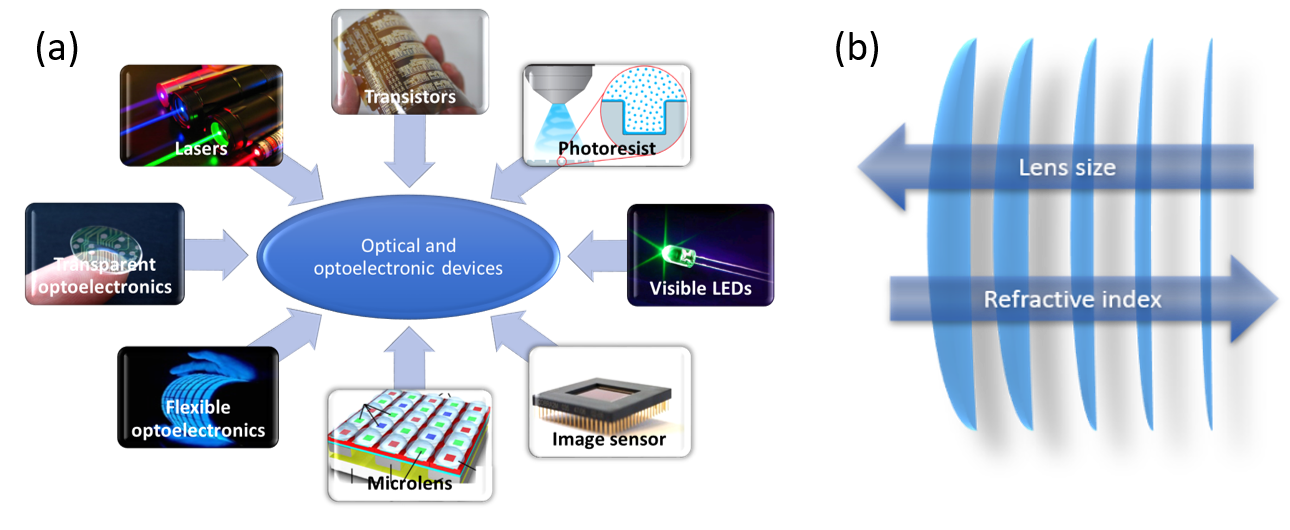
\includegraphics[width=0.95\textwidth]{Chapter-1/Figures/HRIP_apps.png}
\caption{\textbf{(a)} Application range of organic polymers in optoelectronics. \textbf{(b)} Relationship of RI value and lens thickness.}
\label{fig:HRIP_apps}
\end{figure}
%%%

%The traditional, experimentally focused discovery process for new materials is very time-, labor-, and resource-intensive, which limits the number and diversity of candidate compounds that can be explored. 
The two principal challenges in creating new chemistry and materials are that their behavior is governed by complicated structure-property and structure-activity relationships \cite{Selassie2003,Muller2005,LeBaillydeTilleghem2007}, and that chemical space is practically infinite \cite{Lipinski2004,Kirkpatrick2004,Dobson2004}. 
Traditional experiment-driven trial-and-error approaches are increasingly ill-equipped to meet these challenges on their own, in particular since advanced systems require more and more intricate property profiles \cite{Zvinavashe2008,Scior:2009-11,Schneider2010}. 
Progress thus tends to be slow and incremental, in particular for advanced materials systems, which require more and more intricate property profiles. However, chemical and materials research has been undergoing a significant transformation in recent years that can alleviate many of these shortcomings: After decades of continuous advances in methods, algorithms, and computer hardware, the fields of modeling and simulation have reached a tipping point, and they are finally at a stage where they can make accurate predictions for systems that are both realistic and relevant. Progress is now increasingly driven by computational studies, which have become crucial assets in the pursuit of next-generation materials and chemistry. By making guiding predictions, they can significantly boost the efficiency of research endeavors, and uncover promising targets for investigations in the laboratory (see, \eg  Ref.\ \cite{cep01,Sokolov2011,Hachmann2011,Olivares-Amaya2011,Amador-Bedolla2013,Hachmann2014,Pyzer-Knapp2015,Lopez2016}). The White House Materials Genome Initiative (MGI) \cite{NationalMaterials2011} underscores the value of integrated joint ventures between experimentalists and theoreticians in tackling complex discovery and design challenges and delivering revolutionary new materials. That being said, the usual focus on individual compounds has so far been limiting the utility of computational research. While there is obvious value in characterizing particular systems of interest, the insights gained in these small-scale studies cannot easily be transferred or generalized.

Our group is developing a data-driven and rational design framework for accelerating the discovery and design of new chemicals/materials. In this dissertation, I deploy this framework to identify new polymer systems with superior optical properties, specifically the high-refractive-index polymers (HRIPs).


\section{Data-Driven Design of Chemical Systems and the Exploration of Chemical Space}

% introduce data-driven research; point to MGI and other high-profile initiatives for support of promise 
The shift towards a data-driven discovery and rational design paradigm (cf.\ Fig.\ \ref{fig:4th_pillar}) promises to mitigate many of the inefficiencies and shortcomings that are still prevalent in contemporary chemical research. 
% point to MGI and other high-profile initiatives as authorities for support of premise 
There is now a growing agreement on the value of incorporating modern data science -- the 4th pillar of science -- into chemical research, and this development has been recognized by high-profile funding programs such as the MGI \cite{NationalMaterials2011}.
% explain problem setting 
Yet, despite impressive pioneering efforts (\eg  \cite{Hansen2013a,Huan2015,PhysRevB.87.219902,doi:10.1021/cm503507h,Behler2007}), 
there is still a distinct disconnect between the promise of this approach and the realities of every-day research in the chemistry community, where data-driven work does not yet play a significant role. 

\begin{figure}[htbp]
	\centering
	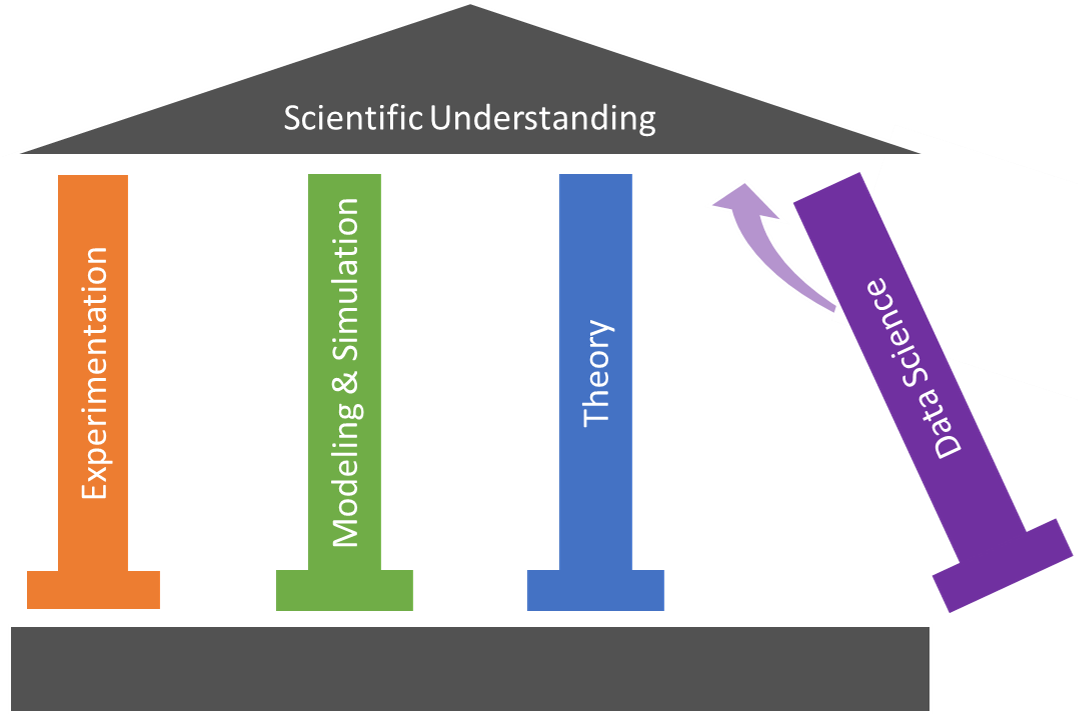
\includegraphics[width=0.7\textwidth]{Chapter-1/Figures/4th_pillar.png}
	\caption{The rise of data science as the 4th pillar of science.}
	\label{fig:4th_pillar}
\end{figure}

\subsection{Group's Approach for Data-Driven \textit{In Silico} Research}
%% Copied from the Molecular Simulation paper
We have developed a basic template for data-driven \insilico\ research, which addresses the inherent challenges in the discovery and design of new chemistry, in particular as part of integrated joint ventures with experimentalists. It provides the foundation and framework for our research program, and its rationale can be summarized as following: 
\begin{itemize}
	\item Using computational modeling and simulations, we can rapidly and efficiently assess the properties, behavior, and performance potential of candidate compounds, materials, and/or chemical transformations for a given problem setting \cite{Olivares-Amaya2011,Wen2012,Stevanovic2014}.
	\item By combining modeling and simulation with high-throughput screening techniques, we can characterize candidates on a massive scale. These studies naturally lead to big data scenarios \cite{Potyrailo2011,Hachmann2011,Hachmann2014,Gunter2012,White2013}.
	\item Using modern database technology, we can readily store and access the resulting data sets, \eg  to identify candidates with desired property combinations for on-demand applications \cite{Blum2011,Ruddigkeit2012}.
	\item In addition to the immediate information obtained for these thousands or even millions of candidates, we can mine the generated data in its entirety. Using machine learning, we can gain insights into the mechanisms that determine their characteristics and cast these findings into predictive models \cite{Rupp2012,Pilania2013,Mansbach2015}.
	\item By identifying these design rules as well as high-value moieties, building blocks, structural patterns, or more general features, we can accomplish the \denovo\ design of next-generation candidates \cite{Pegg2001,Proschak2009,Nakamura2012}. Using the predictive models, we can conduct hyperscreenings, \ie screenings based on data-derived models that typically surpass the scale of the original screenings (based on physics-derived models) by several orders of magnitude.
	\item Experimentalist partners can pursue the top candidates from the (hyper-)screening and/or \denovo\ design. This guidance allows the experimentalists to focus on highly promising targets and avoid wasted efforts on unpromising ones \cite{Sokolov2011}. Additional in-depth modeling and simulations can contribute further insights to the experimental findings, which allow for the advanced optimization of lead candidates. 
	\item The experimental results can be included as training data in the machine learning approaches. In addition, they can be used to validate, benchmark, calibrate, and potentially improve the physics-based modeling and simulation protocols, which closes the design loop \cite{Hartenfeller2011a}. 
\end{itemize}

\subsection{Software Ecosystem for Materials Discovery}

Our group has identified four components that are critical for the efficient discovery of materials with targeted properties. These four components are being developed in the group as four different software packages (see Fig.\ \ref{fig:ecosystem}):
 
\begin{figure}[htbp]
	\centering
	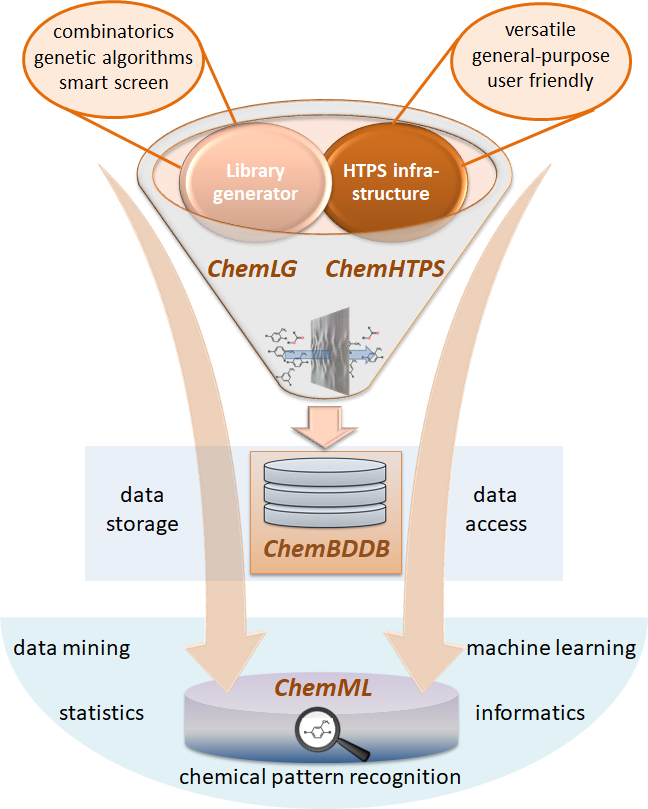
\includegraphics[width=0.6\textwidth]{Chapter-1/Figures/ecosystem.png}
	\caption{Schematic and connectivity of the software ecosystem comprised of the \chemlg , \chemhtps , \chembddb , and \chemml\  codes.}
	\label{fig:ecosystem}
\end{figure}

\begin{enumerate}
	\item \textbf{\chemlg: Screening library generator \cite{Afzal2018b}.} A prerequisite for the high-throughput exploration of chemical space is access to suitable, large-scale screening libraries. We have developed a corresponding generator for compound and material candidate libraries. We discuss in detail the underlying concepts of \chemlg\ in the Chapter 4 and provide case studies where \chemlg\ was successfully applied. I developed \chemlg\ primarily for the creation of high RI polymer candidates.
	\item \textbf{\chemhtps: Virtual high-throughput screening infrastructure \cite{Afzal2018c}.}  \chemhtps\ is a suite for performing large-scale simulations on high-performance computing clusters. This suite supports various quantum chemistry and molecular modeling codes including Q-Chem, ORCA, GROMACS, and LAMMPS. I co-developed \chemhtps\ infrastructure along with William Evangelista. 
	\item \textbf{\chembddb: Database infrastructure \cite{Shirish2018}.} The use of modern databases is of particular importance in the context of data-intensive research. Despite their great utility and despite being essential for projects that accumulate large data sets, they are still rarely employed in chemical research. Our group has developed a database platform to store and provide access to the various results in a centralized fashion. The database also serves as the focal point for the information exchange within the project team and potential external collaborators, as well as for the coordination of the different project components. The developers of \chembddb\ are Aditya Sonpal and Shirish Sivaraj.
	\item \textbf{\chemml: Data analysis, mining, and modeling infrastructure \cite{Haghighatlari2017}.}  \chemml\ suite includes data analysis, mining, and modeling capabilities that allow us to apply state-of-the-art machine learning and informatics methodology to chemical and materials data sets. Using \chemml, we can identify underlying structure-property relationships which are key to create new and more targeted candidate libraries. The primary developer of \chemml\ is Mojtaba Haghighatlari.
	
\end{enumerate}


\subsection{Discovery of High-Refractive-Index Polymers}

Harnessing the potential of organic polymers in optical and optoelectronic industries has been quite limited because these applications require materials to have RI greater than 1.7, while carbon-based polymers inherently have RIs between 1.3 and 1.5. As a result, there is an incentive to discover new high-refractive index polymers for the aforementioned applications. According to the Lorentz-Lorenz equation, the incorporation of substituents with a high molar refractivity and low molar volume can increase the RI values of these materials. This suggests that the ability to tailor the molecular structure of polymers is the key to increasing their RI values \cite{Liu2009}. On the other hand, tailoring the structure using different functional groups could potentially lead to an infinite number of molecular candidates. It is impractical to empirically characterize a large number of candidates, whereas computational analysis allows greater exploration at a mere fraction of the time and cost. The current work is concerned with creating fast and accurate predictive models for the optical properties of organic polymers, which will guide our experimentalist partners and allow them to target the most promising candidates. The application of above mentioned rational design framework in the current work has allowed us to accelerate the discovery of polymers with high RI values materials.

We have developed an accurate model for the prediction of RI values of polymers based on \firstprinciples\ and molecular modeling techniques. The model is based on the Lorentz-Lorenz equation and thus includes the calculation of polarizability and number density values for the candidate structures. In this scheme, we compute the molecular polarizability using \firstprinciples\ electronic structure theory (DFT) and the number density using molecular modeling (MD). The synergistic combination of DFT and MD resulted in a successful and economical model for RI prediction. We validated the RI model using experimental RI values of 112 non-conjugated polymers, which shows that the model is in a good agreement ($R^2$=0.94) with the experimental results \cite{Afzal2018a}. Further details of the model and its validation will be discussed in Chapter 2.

In the RI prediction model, we apply computationally expensive DFT computations. While the choice proved remarkably successful, it represents the bottleneck step in our RI protocol due to computational inefficiency. It thus limits the utility of the overall approach, particularly in the context of virtual high-throughput screenings of large-scale candidate libraries. Therefore, we have systematically benchmarked several DFT model chemistries to find one that optimizes the balance between accuracy and efficiency in the target compounds space. We further compare the results for non-conjugated and conjugated polymers, offer guidance for method selection, and analyze the errors that propagate into the RI predictions. We will discuss the details of the benchmarking study in Chapter 3. 

In search of candidates with high RI values, we created a library of polymers using the \chemlg\ software. In this work, we selected polyimides as a model polymer and created a library of novel polyimides based on the building blocks suggested by our experimental collaborators. We provide an exposition of \chemlg\ software package in chapter 4. The resultant library of polyimides consists of 270,000 candidates. Application of our rational design framework resulted in more than 2000 polyimides with RI values greater than 1.8. The results from the study are presented in Chapter 5.

A large-scale exploration of chemical space will not only identify exceptional molecular targets but also allow us to identify underlying patterns and global trends. These structure-property relationships can aid in the inverse design of materials with specific properties. To achieve this, we created a massive library of 1.5 million small organic molecules and evaluated their properties. Characterization of candidates on such a large scale was possible by the application of advance machine learning techniques. Using the big data obtained form this work, we identified design rules as well as high-value building blocks, and structural patterns that correlate with optical properties. Additionally, we uncovered regions in chemical space where we can maximize the optical properties of organic molecules. These guidelines allow us to target specific molecular motifs and create the next generation of materials with exceptional properties. We present the results from this large-scale exploration in Chapter 6.

This dissertation demonstrates that the developed rational design framework is a powerful tool. The exploration of high-refractive-index polymers is one example for applications problems and I spearheaded this project as part of my dissertation.

\chapter{Accurate Prediction of the Refractive Index of Organic Polymers}

We present an efficient computational protocol for the accurate prediction of RI values in polymers to facilitate \insilico\ studies that can guide the discovery and design of next-generation high-RI materials. Our protocol is based on the Lorentz-Lorenz equation and is parametrized by the polarizability and number density values of a given candidate compound. In the proposed scheme, we compute the former using \firstprinciples\  electronic structure theory and the latter using an approximation based on van der Waals volumes. The critical parameter in the number density approximation is the packing fraction of the bulk polymer, for which we have devised a machine learning model. We demonstrate the performance of the proposed RI protocol by testing its predictions against the experimentally known RI values of 112 optical polymers. Our approach to combine \firstprinciples\  and data modeling emerges as both a successful and highly economical path to determining the RI values for a wide range of organic polymers.

We thank Prof. Chong Cheng for helpful discussions on the scope of high RI polymers and synthetic feasibility of new polymers. The results of this study were published in ‘M. A. F. Afzal, C. Cheng, J. Hachmann, J. Chem. Phys. 128 (2018), 144101’ \cite{Afzal2018a}, and this chapter is based on our exposition in this paper. 

\section{Introduction}
% Provide the general context: list different kinds of organic materials, state wide-ranging importance, discuss unique or desirable properties compared to conventional materials [keep this relatively short - maybe 2-3 sentences or so]
Organic small molecules, oligomers, and polymers are emerging materials and of significant interest for numerous fields of application due to their unique or otherwise desirable properties \cite{Higashihara2015}. Unlike most conventional inorganic materials, they are generally flexible, light-weight, mechanically stable on impact, easy to process, and inexpensive to produce \cite{Lu2005,Zimmermann1993}. Perhaps most importantly, their properties can be tailored towards specific demands by controlling their molecular structure \cite{Liu2009}.
% Narrow down the context: Applications of organic polymers with a focus in optics and optoelectronics; give a number of examples [keep this relatively short - maybe 2-3 sentences or so]
A particular area of interest is the application of organic materials in optic and optoelectronic devices \cite{Lei2014}, such as (image) sensors \cite{Angione2011, Voigt2011}, displays \cite{Ummartyotin2012}, and light sources (including organic light-emitting diodes) \cite{Xiang2017}, in which they can be introduced \insitu\  as microlenses \cite{Nishiyama2009}, waveguides \cite{Kokubun1993}, microresonators \cite{Wei2016}, interferometers \cite{Rodriguez2001}, anti-reflective coatings \cite{Singaravalu2013}, optical adhesives \cite{Kim2013}, and substrates  \cite{Kim2015}. Some of the optical properties that are relevant for these applications are the refractive index (RI), Abbe number, birefringence, absorption spectrum, and color \cite{Sun2008}.   

% Zoom in on refractive index as an important optical property. Mention the importance of high refractive index (>1.7) materials 
The RI value dictates the shape and size of many optical components, in particular those with lens function. Most of the aforementioned applications require materials with large RI values (\ie  larger than 1.7), and there are several applications that require very large ones (\ie  larger than 1.8) \cite{Jintoku2014}. Unfortunately, the vast majority of organic polymers only offer RI values ranging from 1.3 to 1.5 \cite{Liu2009} (compared to inorganic materials, which can feature values up to $\sim$4). 
% Now that we have established that this is an interesting and relevant field, introduce various strategies to increase the RI value in organic materials, and why we are not there yet
The development of high-RI polymers has thus gained attention, and several approaches have been proposed to overcome the RI-value limitations of typical organic polymers. They include the notion to incorporate highly polarizable moieties, such as rigid aromatic fragments \cite{Seto2010}, heteroatoms \cite{Griebel2014,Tojo2013}, or organometallics \cite{Ho2009}, into the polymer scaffold. Another strategy that has been pursued is to reinforce the polymer matrix with metal alkoxides (\eg  \ce{TiO2}, \ce{Fe3O4}) \cite{Liu2013,Parke2013} or other high-RI molecules (\eg  \ce{ZnS}, diamondoids) \cite{Zhang2014,Robello2013}. While these approaches have resulted in a few systems with RI values between 1.6 and 1.8, most of them are of limited utility for practical applications due to a variety of materials, processability, or preparation issues \cite{Liu2009}. Increasing the RI values of organic polymers beyond 1.8 has remained a completely elusive task and continues to be an important challenge in synthetic chemistry \cite{Griebel2014}. 

% Introduce the problem setting that this paper tries to address, i.e., explain the limitations, shortcomings to the traditional, experimental discovery process for high-RI polymers
The traditional, experimentally focused discovery process for new materials is very time-, labor-, and resource-intensive, which limits the number and diversity of candidate compounds that can be explored. Progress thus tends to be slow and incremental, in particular for advanced materials systems, which require more and more intricate property profiles.
% Make case for in silico research in order to overcome shortcomings by supporting, guiding experimentalists, mention MGI; don't bash experiment but show how joint ventures are the path to progress [you can potentially reuse some of the text from my CAREER proposal here; don't go into technical detail but stay with a big picture level]
However, chemical and materials research has been undergoing a significant transformation in recent years that can alleviate many of these shortcomings: After decades of continuous advances in methods, algorithms, and computer hardware, the fields of modeling and simulation have reached a tipping point, and they are finally at a stage where they can make accurate predictions for systems that are both realistic and relevant. Progress is now increasingly driven by computational studies, which have become crucial assets in the pursuit of next-generation materials and chemistry. By making guiding predictions, they can significantly boost the efficiency of research endeavors, and uncover promising targets for investigations in the laboratory (see, \eg  Ref.\ \cite{cep01,Sokolov2011,Hachmann2011,Olivares-Amaya2011,Amador-Bedolla2013,Hachmann2014,Pyzer-Knapp2015,Lopez2016}). The White House Materials Genome Initiative \cite{NationalMaterials2011} underscores the value of integrated joint ventures between experimentalists and theoreticians in tackling complex discovery and design challenges and delivering revolutionary new materials.
%\textcolor{red}{
A prominent example in the context of optical materials is the work by Ramprasad and co-workers \cite{Huan2016,Sharma2014,Mannodi-Kanakkithodi2016}, which we will use as a reference point.
% }

% Point out the prerequisite for this approach: having a suitable computational protocol for predicting the RI of polymers, i.e., developing this paper is about developing such a protocol
A prerequisite for the computationally-driven development of new materials is access to suitable (\ie  accurate and efficient) computational protocols for the target property within a compound space of interest. This paper presents such a protocol for the prediction of RI values of organic polymers. One of the distinctive feature of this protocol compared to prior work by others \cite{Huan2016,Sharma2014,Redmond2011,Park2011} is that it fuses \firstprinciples\  and data modeling. 

% outline of paper
In Sec.\ \ref{sec:methods}, we introduce the physical foundations of the proposed protocol (Sec.\ \ref{subsec:lorentzlorenz}), 
motivate a number of assumptions and approximations that are used (Sec.\ \ref{subsec:polarizability} and \ref{subsec:numberdensity}), and discuss the details of the employed computational approach (Sec.\ \ref{subsec:compdetails}). In Sec.\ \ref{sec:results_discussion}, we present and discuss results for the different components that comprise the protocol (Sec.\ \ref{subsec:polarizability_results}, \ref{subsec:numberdensity_results}, and \ref{subsec:packingfractions_results}) as well as the overall protocol itself (Sec.\ \ref{subsec:RI_results}). In each case, we evaluate the predictive performance of our model by comparing its results with data from a validation set of experimentally known compounds. Sec.\ \ref{subsec:interplay_results} provides a discussion of the interplay between the physical parameters of our model. Our findings are summarized in Sec.\ \ref{sec:conclusions}.



\section{Background and Methods}
\label{sec:methods}
\subsection{Lorentz-Lorenz Equation}
\label{subsec:lorentzlorenz}
% Connection of the refractive index with the polarizability and number density via the Lorentz-Lorenz equation [logic/argument from presentation slides]
The RI value ($n_r$) is defined as the ratio between the speed of light in vacuum ($c_0$) and in a given material ($c$). For non-magnetic materials, the RI is thus the square root of its relative permittivity 
% \textcolor{red}{
or dielectric constant 
% }
($\epsilon_r$), \ie 
$$n_r=\dfrac{c_0}{c} = \sqrt{\epsilon_r}.$$
The permittivity is a function of the polarizability ($\alpha$) and using the Lorentz local field approximation, it can be written as
$${\epsilon{}}_r=\frac{1+2\alpha{}N/{3\epsilon{}}_0}{1-\alpha{}N/{3\epsilon{}}_0},$$
where $N$ is the number density, \ie   the number of molecules per volume. It follows that the RI is
$$n_r=\sqrt{\frac{1+2\alpha{}N/{3\epsilon{}}_0}{1-\alpha{}N/{3\epsilon{}}_0}},$$
which is a version of the Lorentz-Lorenz equation (equivalent to the Clausius-Mossotti relation). It follows, that the Lorentz-Lorenz equation connects the macroscopic RI value of a bulk material to the electronic polarizability $\alpha$ and number density $N$ of its molecular constituents.
% Give a brief summary of the physical basis of the RI protocol 
The Lorentz-Lorenz equation thus offers a route to calculating the RI value of a material \via\ $\alpha$ and $N$, and we use it as the physical basis for the proposed computational protocol (for a detailed discussion of this approach see App.
\ref{appendix:A}).  


\subsection{\textit{First-Principles} Molecular Polarizability Calculations}
\label{subsec:polarizability}
% Introduce general notion of molecular polarizability calculations, issue of dispersion
The polarizability $\alpha$ of a compound can be obtained from quantum chemical linear response calculations. An array of electronic structure methods has been used to determine the polarizability values of various materials \cite{Ando2006,Rocquefelte2004,Jensen1983,Rabah2003,Amrani2006,Reshak2014,Azam2013}, including organic polymers \cite{Ksianzou2006,Zeinalipour-Yazdi2008,Yu2007}. Polarizability is generally a frequency-dependent (\ie  dynamic) property as shown in Fig.\ \ref{fig:pol_wl}. Frequency-dependent polarizability is relatively hard to compute, as it formally involves solving the time-dependent Schr\"odinger equation and/or scanning through the range of relevant frequencies \cite{Rao2013}. Consequently, only relatively few studies consider the polarizability dispersion in organic polymers \cite{Rowan2011,Lenz2011}. 

\begin{figure}[htbp] 
	\centering
	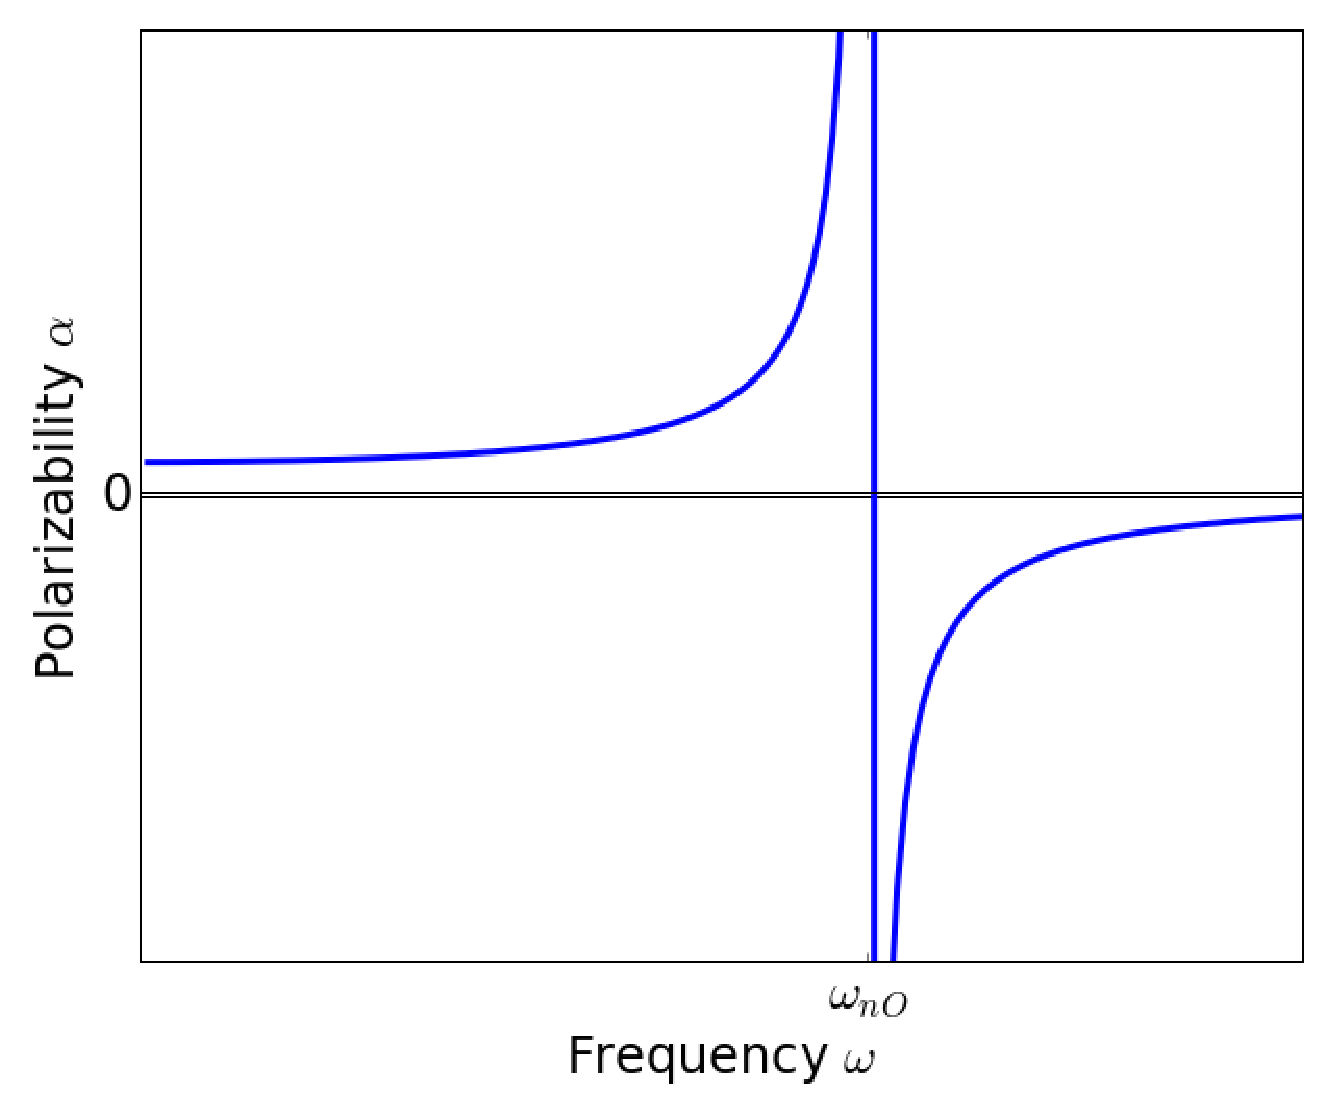
\includegraphics[width=0.6\textwidth]{Chapter-2/Figures/RI_vs_freq.eps}
	\caption{Dispersion characteristic of the polarizability: Excited states are marked by singularities, and in the frequency range below, the polarizability converges asymptotically towards the constant static polarizability value.} 
	\label{fig:pol_wl} 
\end{figure}  

% go to RI, argue why we get away with using frequency independent solution/static polarizability
From the frequency dependence of the polarizability follows that the RI is also a frequency-dependent property. However, the variation of both polarizability and RI in the visible frequency region is in fact often relatively small \cite{Robello2013}, as long as low-lying excited states are absent. Since the latter would render a material unsuitable for optical applications anyways, we generally do not consider materials that exhibit them. Large variations can be observed in the ultraviolet region where resonances with the excited state manifold become a dominant feature, but since stability considerations prohibit organic polymers to be used for high-energy applications, this is also not a relevant concern. Below the frequency range of the excited states, the polarizability and RI value taper off monotonically (cf.\ Fig.\ \ref{fig:pol_wl}). In most cases, they become essentially constant throughout the visible and infrared range and converge to an asymptotic value \cite{Robello2013}. The asymptotic RI corresponds to the value that can be obtained from the static polarizability. The latter can be computed much more easily than the frequency-dependent value. It only requires a single linear response calculation without explicit time dependence, and is thus much less demanding in terms of computing time and numerical stability. We can conclude that the RI values obtained from static polarizability calculations form a close lower bound for the frequency-dependent values in the relevant spectral range. This approach has been used in the past and has given very good agreement with experimental results \cite{Azim-Araghi2012,Ksianzou2006,Lee2011,Park2011,Zeinalipour-Yazdi2008}.

% move on to challenge of calculating polymer values
Another challenge is to perform the polarizability calculations for quasi-infinite polymers. 
% outline issues: PBC tricky and not realistic, explicit polymer calcs too expensive
Realistic systems are amorphous and may thus not be well represented by periodic boundary condition calculations, while non-periodic calculations on long-chain oligomer models are generally cost-prohibitive. 
% solution via extrapolation scheme: make use of short correlation length, extensivity of optical properties
However, for systems with a relatively short correlation length (\eg  due to finite conjugation and delocalization of the $\pi$-electron backbone), we can expect an early onset of extensivity in the optical properties. We can exploit this behavior through an extrapolation scheme. 
% explain extrapolation scheme, i.e., talk about polymer values from molecular ones: polymer polarizability values can be obtained from small chain oligomers results using extrapolation scheme  
In this scheme, we perform a series of relatively simple monomer and small oligomer calculations until we observe a linear trend in the polarizability results, based on which we can project 
%from the molecular results 
to the polymer limit.

% talk about DFT, cost vs accuracy -> basis set dependence, scaling, prior benchmark study
The molecular polarizability calculations in the proposed protocol utilize Kohn-–Sham density functional theory (DFT) for its advantageous trade-off of cost and accuracy \cite{Neese2009}. The former includes its low-order polynomial scaling with system size and its relatively modest basis set demands (compared to high-level wavefunction methods).
%; the latter has been shown in prior benchmark studies 
% discuss geometries and geometry optimization; justify 
Given the molecular-level disorder in amorphous polymers, we forgo the expensive \firstprinciples\  optimization of idealized geometries of our candidate compounds in favor of an inexpensive molecular mechanics approach. 
% mention that we check for low lying excited states by assessing HOMO-LUMO gap
A simple, yet efficient way to identify (and exclude) compounds with potentially low-lying excited states is to assess the gap between the highest occupied molecular orbital (HOMO) and the lowest unoccupied molecular orbital (LUMO). The HOMO--LUMO gap is a first approximation for the lowest excitation, and it is readily obtained in DFT at no additional cost.  



\subsection{Data Model for the Number Density}
\label{subsec:numberdensity}
% introduce MD as conventional approach to compute number density
The number density $N$ for amorphous polymers is typically computed using classical molecular dynamics simulations. 
% MD is a time consuming and complicated approach that does not scale well for the long-term goal of screening 
However, this approach is relatively cumbersome and computationally demanding.
% we try to avoid it and instead bypass it using the using an approximation based on the Van der Waals volume; mention that for this we need to know the vdW volume and packing fraction 
As an alternative, we pursue an approach based on the molecular volume (approximated by the van der Waals volume $V_{vdW}$), \ie 
$$N=\frac{K_p}{V_{vdW}},$$
where $K_p$ is the packing fraction in the bulk polymer, which has shown good agreement with experimental results in other work \cite{Liu2008a,Terui2004}. 
% mention that there are many different approximations for how to compute the former (list these), but that a comparison indicates that the differences are relatively small so that we utilize a more simplistic scheme 
There are a number of ways to compute the van der Waals volume, ranging from complicated electronic structure calculations with subsequent partitioning of the electron density to simplistic fragment methods \cite{Lu2012,Zhao2003}. A benchmark study that we will detail elsewhere has shown that the differences in results from different methods are generally small. For the present work, we thus adopt the latter, \ie  we calculate $V_{vdW}$ by adding tabulated atomic values \cite{Bondi1964} and subtracting off the overlap in the bonding region. 
% Discuss that packing fraction is given as a constant in the literature but that this is an average with large standard deviation which makes it useless
The average packing fraction $K_p$ for organic polymers is given in the literature as 0.68 \cite{askadski2003}, however, the actual values of different polymers show a significant spread and are known to range at least from 0.5 to 0.8. ($K_p$ is generally also a function of the degree of polymerization, but except for shorter oligomers, this only plays a minor role.)  
% Introduce machine learning approach for the prediction of the packing fraction. Mention on a basic level the choice of approach and motivation
As the average value of this critical parameter is thus essentially meaningless, we have devised a machine learning model to correlate the polymer structure with its packing fraction. Due to the relatively small volume of available training data, we chose a comparatively inflexible (but exceedingly fast) support vector regression (SVR) approach to avoid overfitting. 
% \textcolor{red} {
Modern support vector machines were introduced in 1992 for supervised classification problems and have been a popular machine learning technique since their inception \cite{Boser1992}. A version for regression analysis was added in 1996 \cite{drucker1997,smola2004}. Non-linear SVR prediction models are generated by projecting the training data into a high-dimensional kernel-induced feature space where they become linear regression problems subject to cost functions that penalize prediction errors.
% }


\subsection{Computational Details}
\label{subsec:compdetails}
The polarizability calculations of the proposed protocol use an all-electron, restricted DFT framework with the PBE0 hybrid functional \cite{Adamo1999} in combination with the triple-$\zeta$ quality def2-TZVP basis set by the Karlsruhe group \cite{Weigend2005}. We include Grimme's D3 correction \cite{Grimme2010} to account for dispersion interaction. The proof-of-principle study shown in the following section was carried out using the ORCA 3.0.2 quantum chemistry program package \cite{Neese2012} with default settings. We optimized the geometries of all monomers and oligomers using the universal force field (UFF) \cite{Rappe1992} as implemented in the OpenBabel software \cite{OBoyle2011}. We calculated the van der Waals volumes using Slonimskii's method detailed in Ref.\ \cite{Slonimskii1970}, for which we implemented a Python script.
% detail the ML algorithm and details of the parameters used. Subsequently, give details of the descriptors used for the ML model.
We generated the packing fraction model using SVR within a feature space of 43 constitutional descriptors on a training data set of 84 polymers with experimentally known $K_p$ values compiled from the literature. The available data was divided into 80\% training and 20\% test set for cross-validation. 
The data modeling was performed using \chemml\ \cite{Haghighatlari2017}, our program suite for machine learning and informatics in chemical and materials research. In this work, \chemml\ employed the scikit-learn 0.17 SVR library \cite{scikit-learn} and descriptors from Dragon 7 \cite{Taletesrl2011}.
% Mention ChemHTPS to perform RI calculation on 112 polymers [keep this short to 1-2 sentences and refer to future publications on the details; you don't want to muddy the two stories]. 
The proof-of-principle study involved about 450 individual calculations, which we performed using \chemhtps\ \cite{Afzal2018c}, our program suite for automated virtual high-throughput screening in chemical and materials research.  



\section{Results and Discussion}
\label{sec:results_discussion}
% Results of polarizability calculation of non-conjugated polymers polyethylene (PE) and polystyrene (PS) as example polymers, subsequently known polymers.  
We developed the proposed RI protocol on two common non-conjugated polymers -- polyethylene (PE) and polystyrene (PS) -- as prototype systems. Subsequently, we performed a study of 112 non-conjugated polymers for which experimental RI values are known in order to validate the predictive performance of the RI protocol as well as its individual components. 

\subsection{Polarizabilities}
\label{subsec:polarizability_results}
% Linear dependence and easy extrapolation scheme; point out that this is valid for non-conjugate polymers and that for conjugated ones this may not be the case, cite Dupuis paper
The PBE0/def2-TZVP-D3 polarizability results for PE and PS from monomer to heptamer are shown in Fig.\ \ref{fig:pol_lin}. The linear trend with respect to the number of monomer units $n$ (due to extensivity) is easily recognized. The correlation coefficient $R^2$ for the linear regression is $\gg0.99$. For all cases studied in this work, extensivity was observed for very short oligomer sequences, and we based our extrapolation scheme on the linear regression slope obtained from the monomer to tetramer results.


\begin{figure}[htbp] 
	\centering
	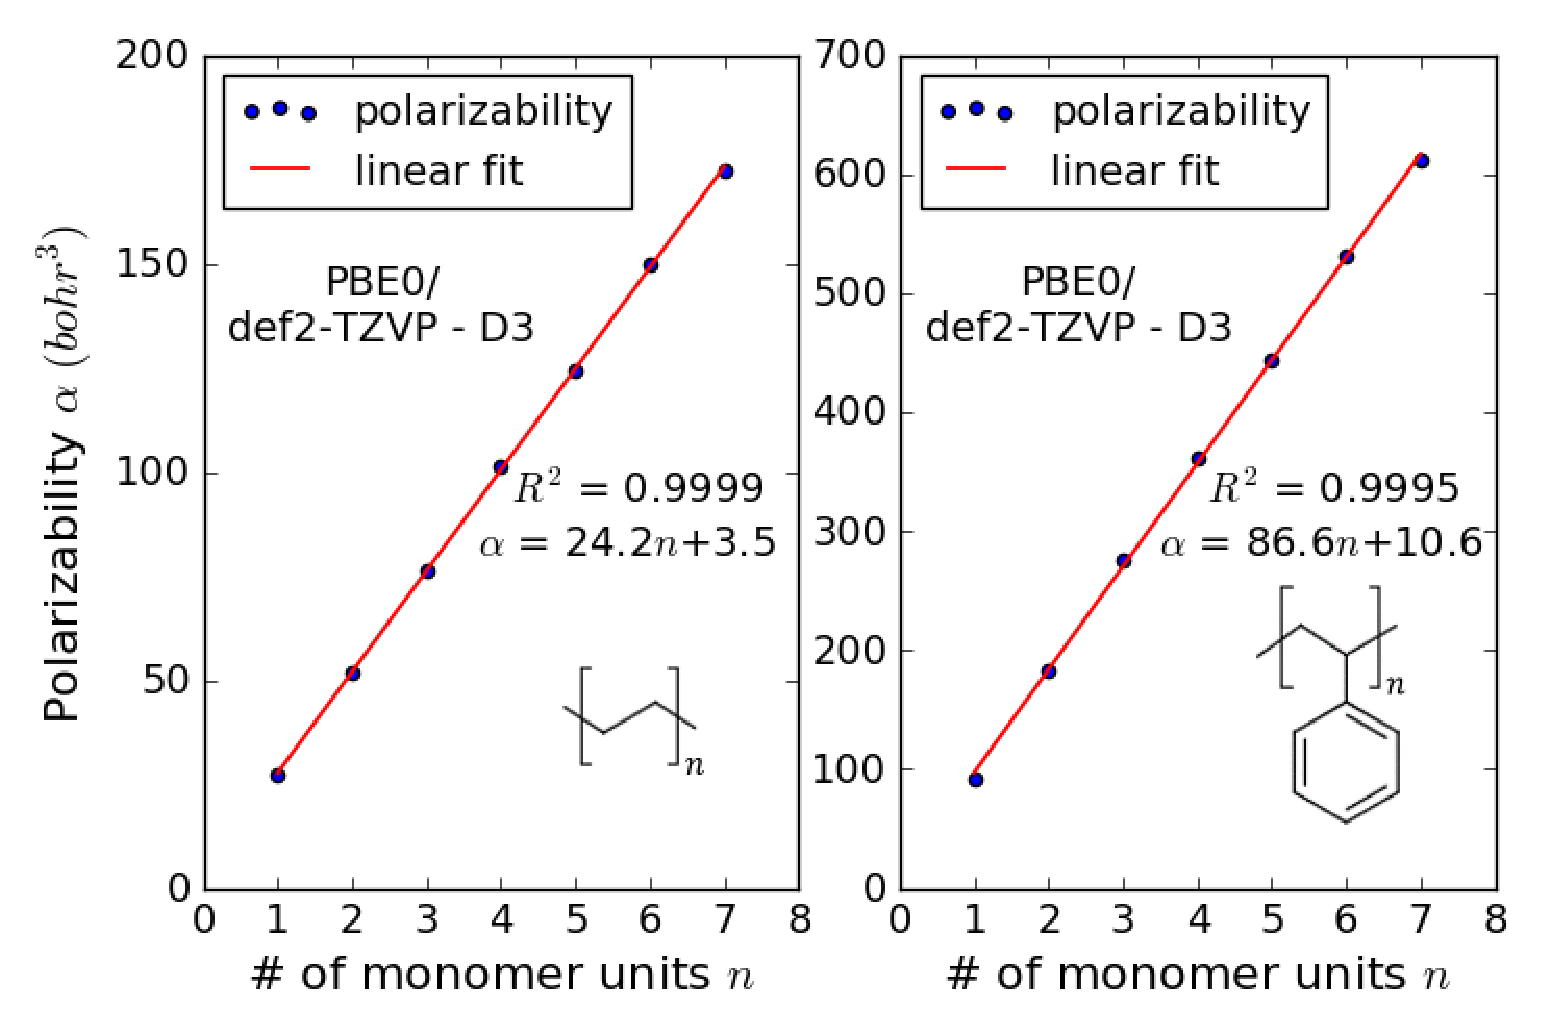
\includegraphics[width=0.75\textwidth]{Chapter-2/Figures/plot_pol.eps}
	\caption{Linear relationship between number of monomer units and polarizability for polyethylene (PE) and polystyrene (PS) as prototypes for non-conjugated polymers.} 
	\label{fig:pol_lin} 
\end{figure}  

Note that for conjugated polymers with longer correlation lengths, the onset of extensivity can occur at significantly longer chain length, \ie  values for a sequence of shorter oligomers will not show a linear trend \cite{Dupuis1988,Mosley1994}. 
% \textcolor{red} {
An example is given in Fig.\ \ref{fig:pol_non_lin}. 
% }
The extrapolation scheme can still be used in these cases, but it requires the calculation of longer oligomer sequences until a linear trend for extrapolation is found. 

\begin{figure}[htbp] 
	\centering
	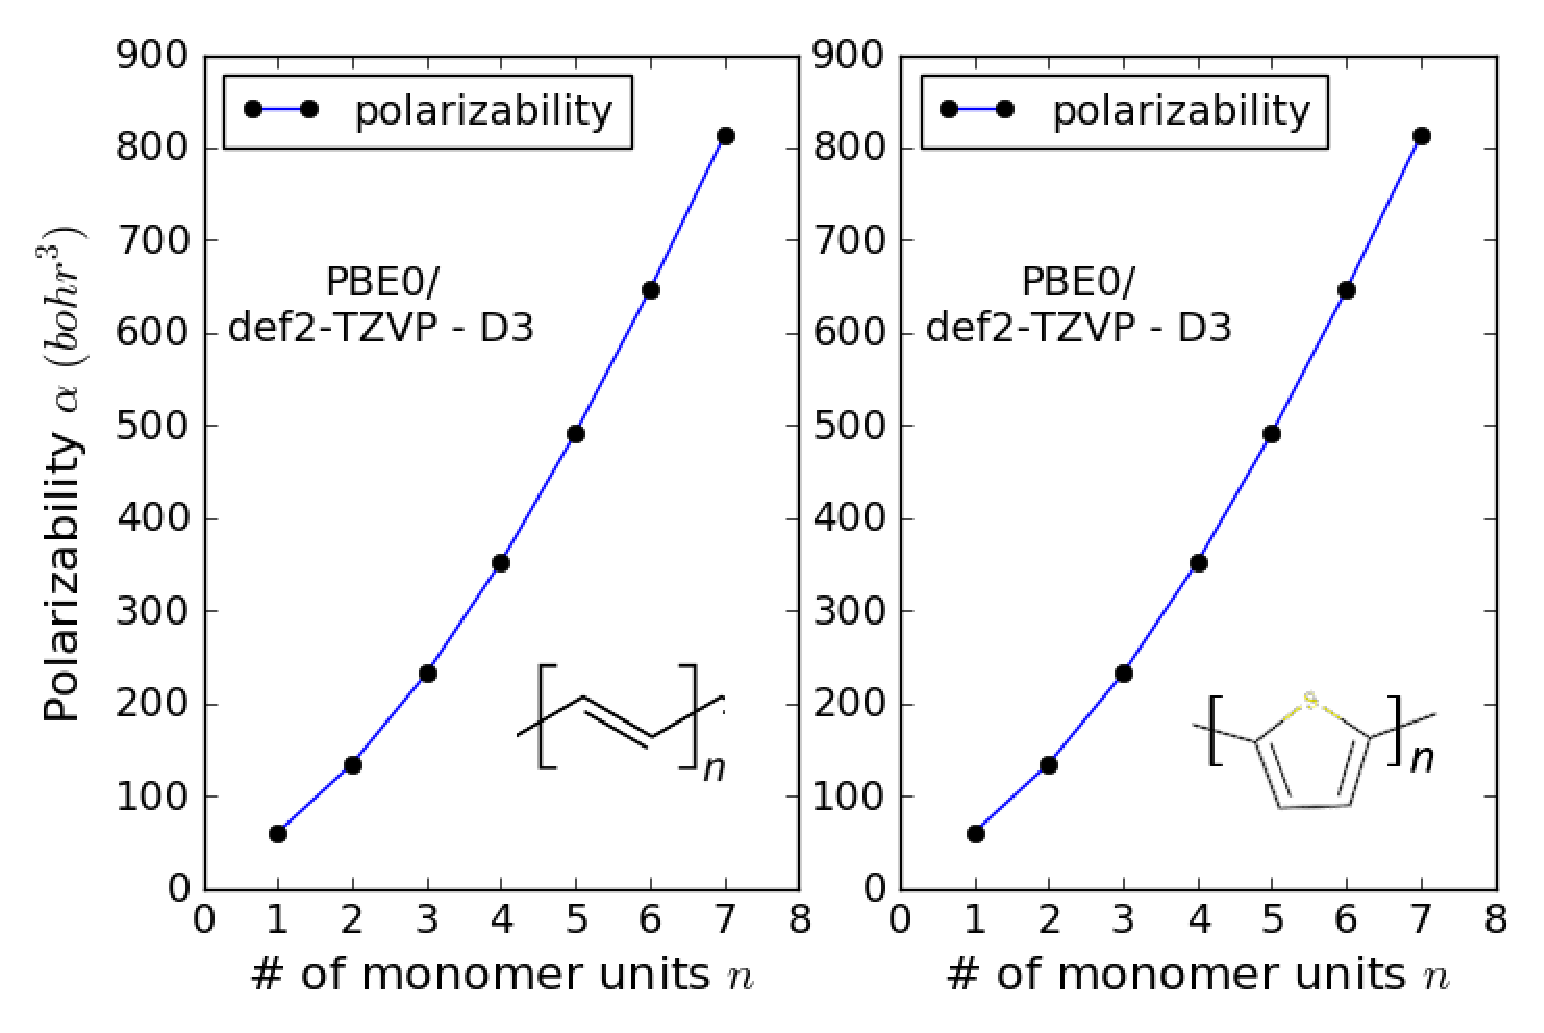
\includegraphics[width=0.75\textwidth]{Chapter-2/Figures/PA_PT_pol.eps}
	\caption{Non-linear relationship between number of monomer units and polarizability for polyacetylene and polythiophene as prototypes for conjugated polymers.} 
	\label{fig:pol_non_lin} 
\end{figure}  



\subsection{Number Densities and Densities}
\label{subsec:numberdensity_results} 
% Results of number density calculation of bulk polymers of PE and PS; this will be straight forward from vdW volume, as we already know the packing fraction of these polymers. 
Using Slonimskii's method we could readily compute the van der Waals volumes $V_{vdW}$ for the prototype systems PE and PS. Assuming the average packing fraction of $K_p = 0.68$, we obtain the number density values $N$ as a function of the number of monomer units $n$ shown in Fig.\ \ref{fig:nden_ex}.  
% Discuss the variation of number density with chain length using the same packing fraction for all oligomer length. 
The plots illustrate that $N$ decreases monotonically with increasing number of monomer units, and the inverse $1/N \propto V_{vdW}$ is evidently extensive. 


\begin{figure}[htbp] 
	\centering
	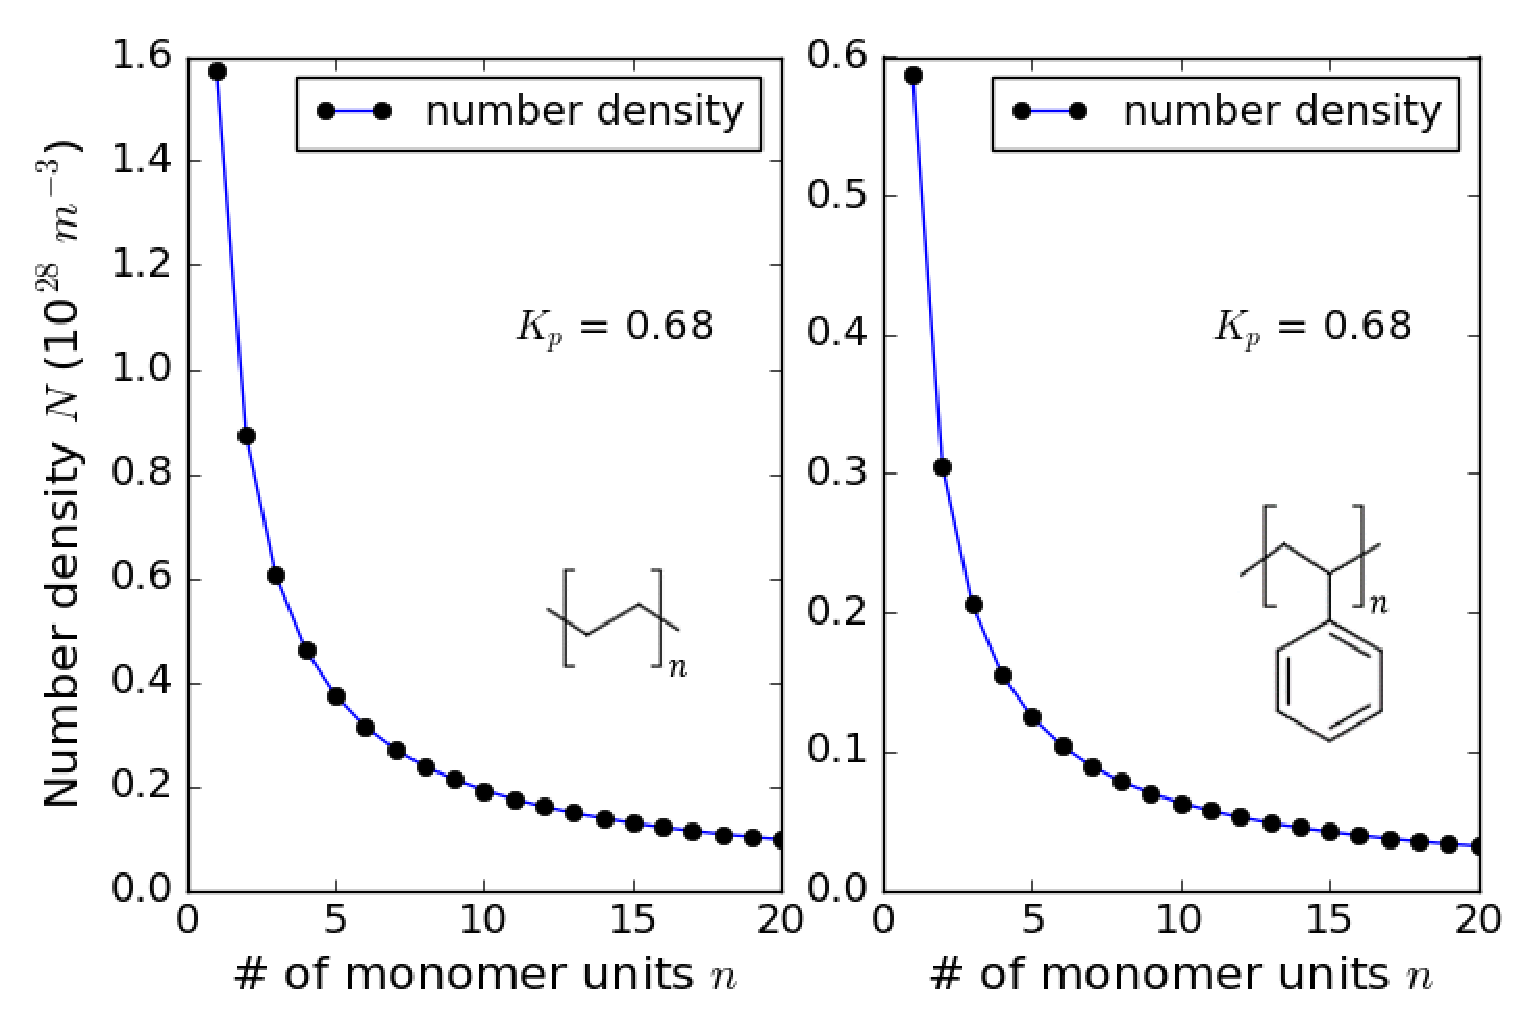
\includegraphics[width=0.75\textwidth]{Chapter-2/Figures/plot_numden.eps}
	\caption{Change of number density values for increasing degree of polymerization for the PE and PS prototype systems.} 
	\label{fig:nden_ex} 
\end{figure} 


Note that we can use this approach to compute another property of interest in organic materials research, \ie  the density $\rho$ of amorphous polymers in the bulk (\via\ $\rho = N \cdot N_A / M$ with the Avogadro number $N_A$ and molecular weight $M$). The density results for our prototype systems are presented in Fig.\ \ref{fig:den_ex}. 
% Discuss the variation of density (asymptotic behavior) with chain length using the same packing fraction for all oligomer length. 
The plots show that $\rho$ increases and ultimately convergences towards asymptotically constant values. This finite size effect due to the terminal groups is typically of limited magnitude. 
% Point out that calculation of density of 50 chain length polymer is a good representation of polymer limit.
The results of the oligomers with $n=50$ offer a good representation of the polymer limit and can thus be used as the default for determining $\rho$. The resulting densities are in very good agreement with experimentally known values \cite{Bicerano2002}. 
% Note that the Bicerano2002 paper reports the density values (gm/cm3) and not the number density values.
We can also use $\rho$ to work backwards and obtain the actual $K_p$ values. For PE and PS we obtain 0.64 and 0.66, respectively, \ie  using the average packing fraction of 0.68 happened to be a valid assumption in these particular cases.


\begin{figure}[htbp] 
	\centering
	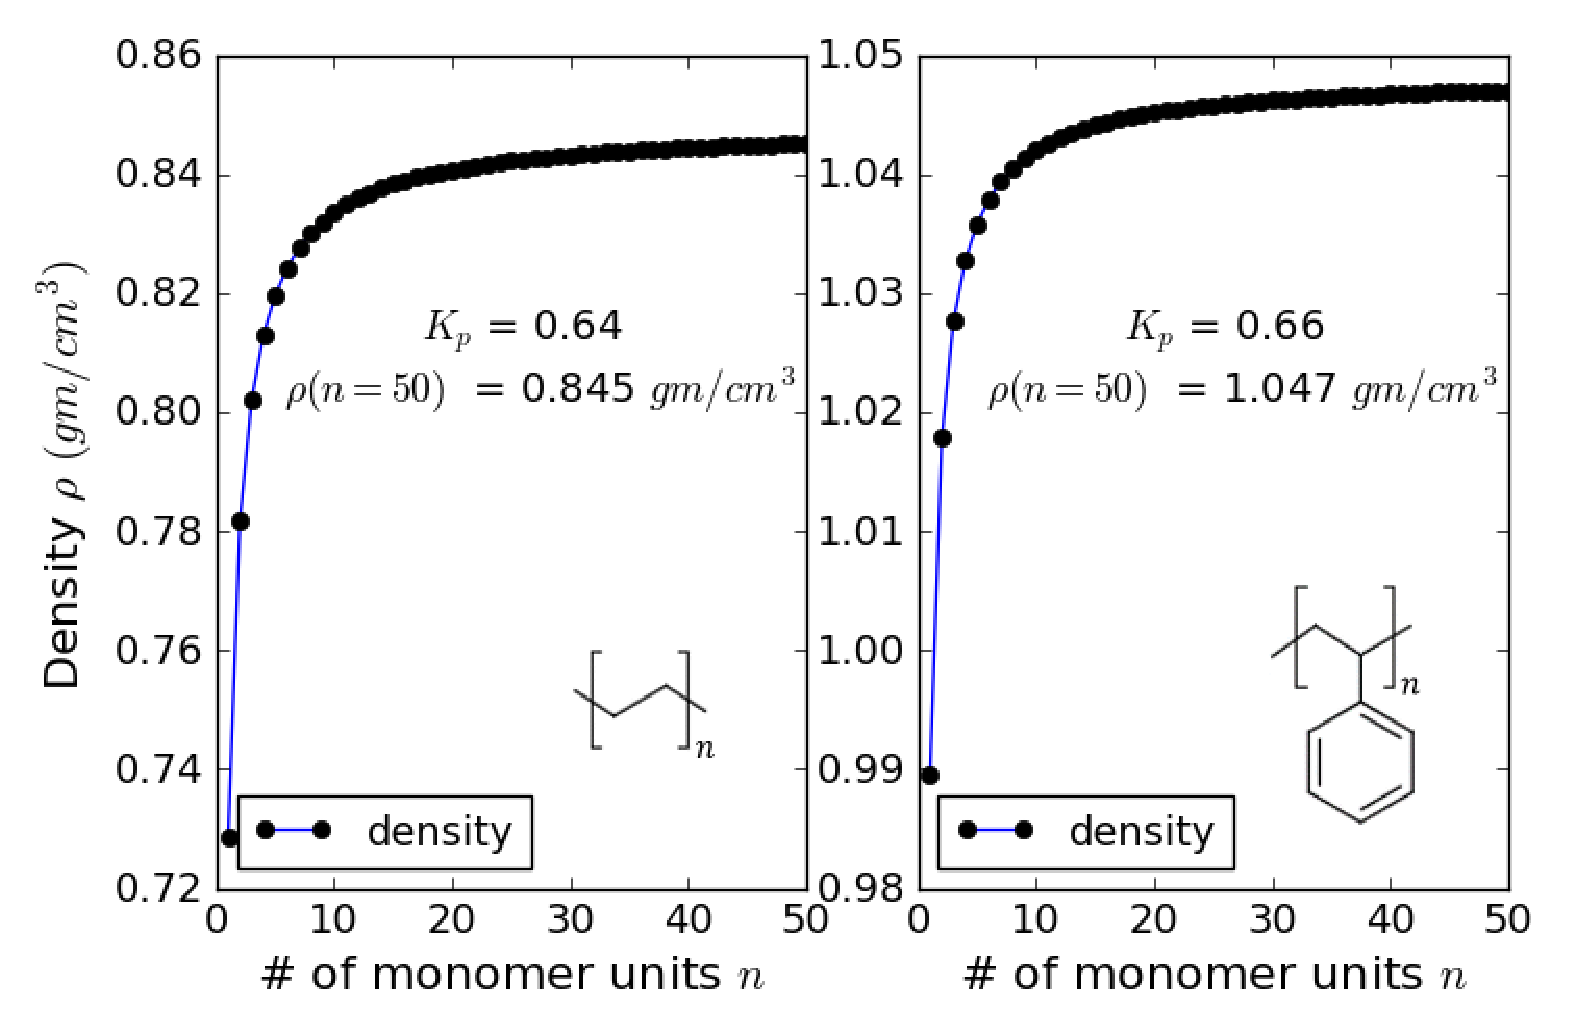
\includegraphics[width=0.75\textwidth]{Chapter-2/Figures/plot_den.eps}
	\caption{Change of density for increasing degree of polymerization for the PE and PS prototype systems. Note the characteristic asymptotic convergence to a constant value.}
	\label{fig:den_ex} 
\end{figure} 



\subsection{Packing Fractions}
\label{subsec:packingfractions_results}
% Explain that the packing fraction of targeted polymers is usually not known and therefore a prediction model is required
As $K_p$ is generally not known and the average value referenced in the literature \cite{askadski2003} is of limited utility, we have devised an SVR data model that correlates the polymer structure with the packing fraction as outlined in Sec.\ \ref{subsec:numberdensity} and \ref{subsec:compdetails}.
% Discuss the histogram of packing fractions of 84 polymers obtained from experimental density values and also on the range of the distribution
Fig.\ \ref{fig:Kp_hist} displays the range and distribution of $K_p$ values for the 84 polymers for which we found experimental results. 
%(either for $K_p$ or $\rho$)
This data -- ranging from 0.53 to 0.79 with an average value of 0.67 -- formed the basis for our data-derived $K_p$ prediction model. (Note that the average $K_p$ for our data set is nearly identical with the average $K_p=0.68$ cited in Ref. \cite{askadski2003}). 

% TODO: Do we have a plot of experimental vs ML K_p? potentially swap against Kp_hist
% Atif: Regarding the comparison of experimental and predicated Kp values, the issue is which graph to show. Should we present the correlation that use complete data for training or the correlation with 80-20 split for training and test respectively? I included a plot  for the latter (Kp_comparison.png and Kp_comparison.eps) in the folder 11/11_RI_prediction/pics/new_pics. I believe showing the histogram and including statistical data for the model would be less confusing.
\begin{figure}[htbp] 
	\centering
	\includegraphics[width=0.6\textwidth]{Chapter-2/Figures/Kp_hist.eps}
	\caption{Range and distribution of experimental packing fraction values for 84 polymers used in the creation of our data-derived prediction model.} 
	\label{fig:Kp_hist} 
\end{figure} 

% Results of SVR model
% Show the results of data modeling for the accurate prediction of packing fraction of polymers using SVR machine learning. Discuss the performance and the speed of the model.
The model gives an $R^2$ of 0.97 for the training and 0.87 for the test set. The performance drop for the latter is reasonable and acceptable given the small size of the available data set.
The computational demand for the $K_p$ prediction model is negligible and results for even large-scale compound libraries can be obtained in minutes on a single processor. 


\subsection{Refractive Indices}
\label{subsec:RI_results}
% Discuss resulting RI model that combines the results from polarizability and number density of these polymers and put in Lorentz-Lorenz equation to get RI values. 
Given the modeling protocols and resulting data for $\alpha$, $V_{vdW}$, $K_p$, and $N$, we use the Lorentz-Lorenz equation to make RI predictions.    
% Results of RI calculation of PE and PS prototype systems and comparison with experimental values; discuss the variation of RI values with the increasing chain length. 
Using the $\alpha$ and $N$ values obtained for our PE and PS prototype systems as shown in Figs.\ \ref{fig:pol_lin} and \ref{fig:nden_ex}, we calculate the RI values and their variation with the number of monomer units $n$ given in Fig.\ \ref{fig:RI_ex}. The RI increases for longer oligomers before reaching a plateau for $n=20$ to $30$. 


\begin{figure}[htbp] 
	\centering
	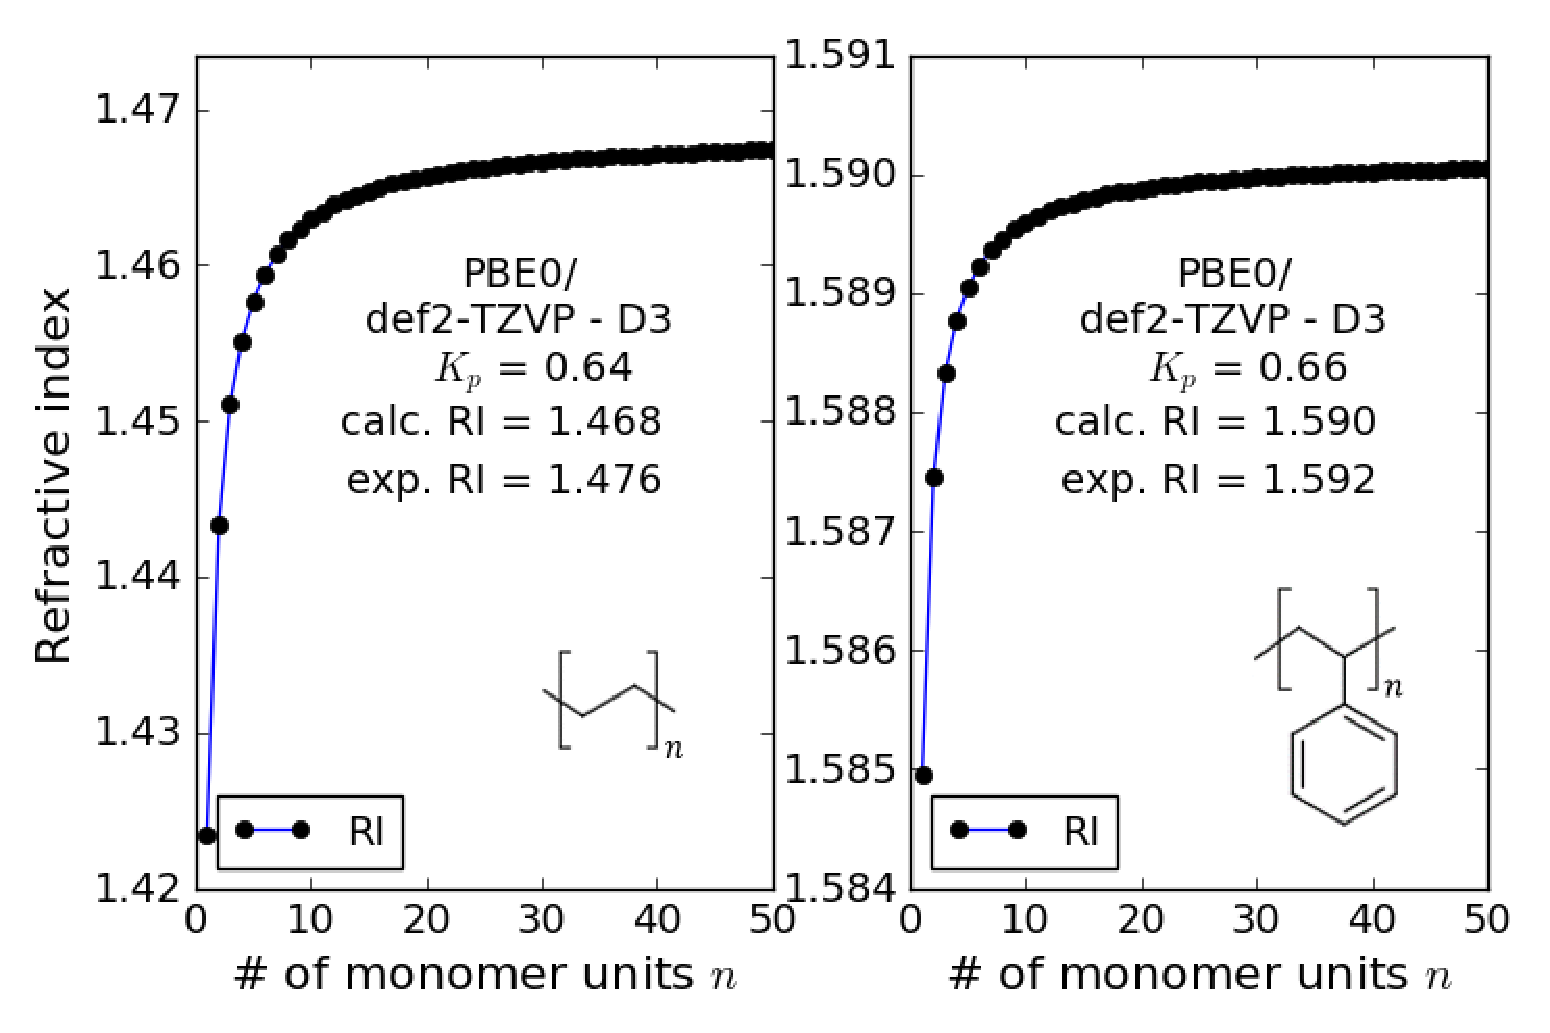
\includegraphics[width=0.75\textwidth]{Chapter-2/Figures/plot_RI.eps}
	\caption{Change of refractive index (RI) with increasing degree of polymerization for the PE and PS prototype systems. Note the characteristic asymptotic convergence to the constant value at the polymer limit, that is in excellent agreement with the experimental data.} 
	\label{fig:RI_ex} 
\end{figure}  


% Comparison with experimental results
Our modeling protocol predicts the RI values for PE and PS to be 1.468 and 1.590, respectively, which is in outstanding agreement with the experimental RI values of 1.476 and 1.592, respectively \cite{Bicerano2002}.
% Now that we have developed a model for the prediction of RI values of polymers, we validate it by testing against the experimental RI values of 112 polymers. 
We further validate our modeling protocol by predicting the RI values of 112 polymers for which we could find experimental data for comparison (see Fig.\ \ref{fig:validation}). 



% \begin{figure}[htbp] 
\begin{figure}[hbpt] 
	\centering
	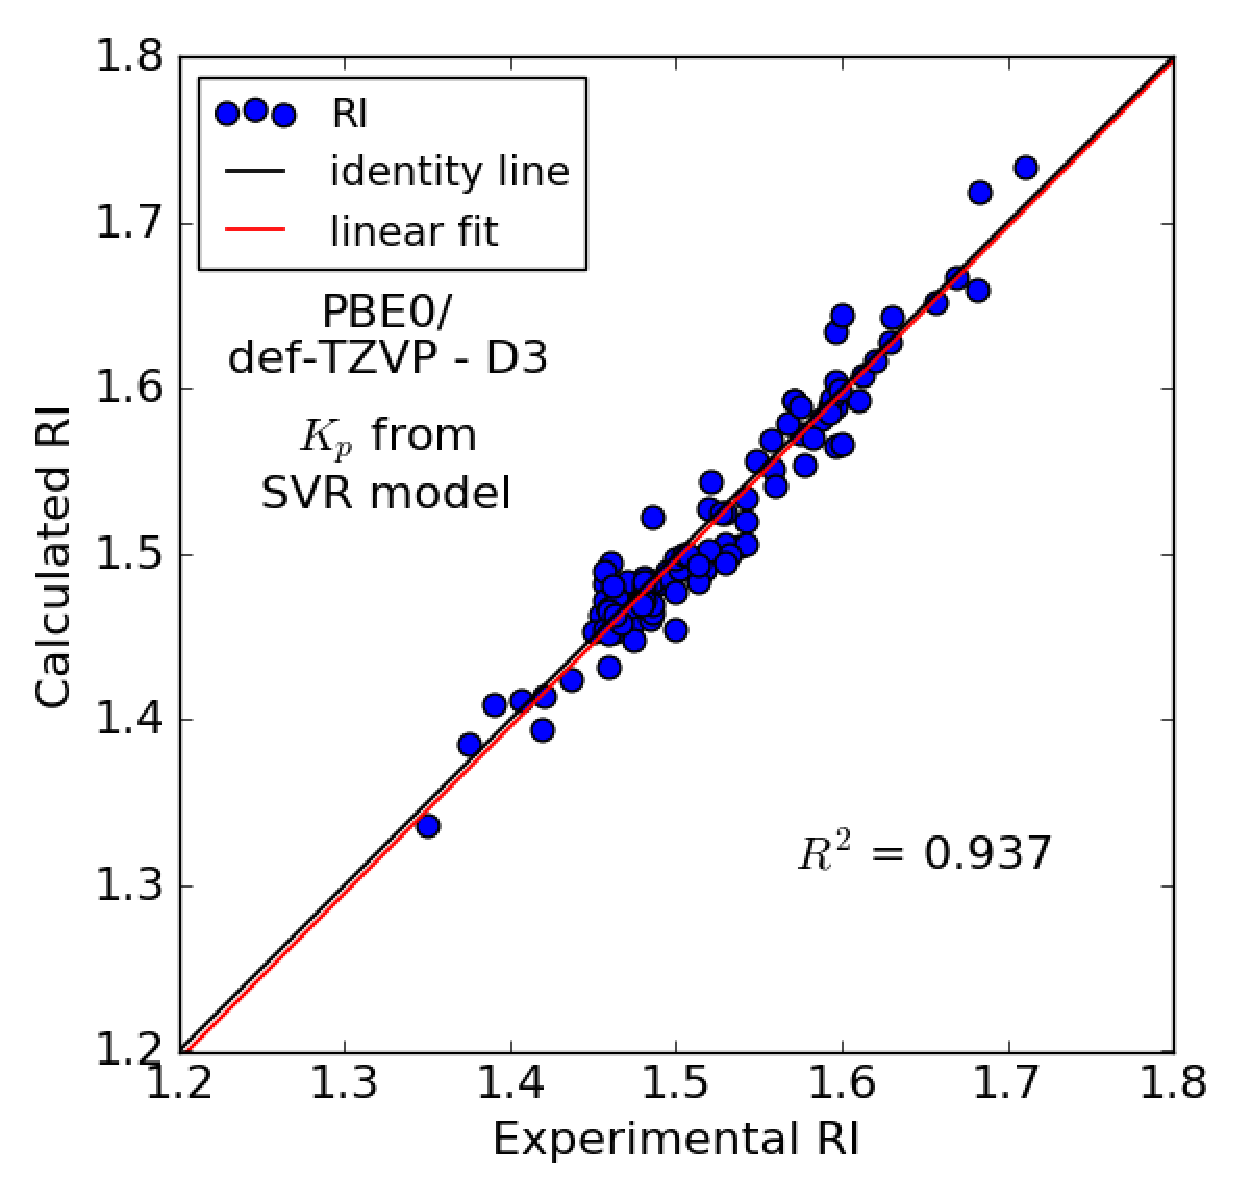
\includegraphics[width=0.6\textwidth]{Chapter-2/Figures/PBE0_Kp_ML.eps}
	\caption{Validation of the proposed RI prediction model (based on the data-derived model for the packing fraction) through comparison with 112 experimental data points.	
	} 
	\label{fig:validation} 
\end{figure} 


% Discuss the performance of the model. 
The $R^2$ of 0.94 shows that the model is in very good agreement with the experimental RI values. The benchmark comparison gives a mean absolute deviation (MAD) of 0.010 (0.9\%), a root mean square deviation (RMSD) of 0.018 (0.1\%), and a maximum deviation (MaxD) of 0.045 or 3.0\%, respectively, \ie  our modeling protocol is quite accurate and affords at least semi-quantitative predictions (in particular since typically only two decimals in the RI values are considered as significant). The average deviation (AD) is very small with +0.004 (+0.3\%), \ie  our model is not significantly biased towards systematic over- or under-predictions. A result of particular importance for studies that focus on candidate rankings rather than quantitative predictions for individual candidates is that the trends in the data are generally well captured. We stress that the experimental RI data is independent of the data used for the creation of the SVR model for $N$, \ie  the SVR model was not biased towards providing good RI results.

% TODO: add to Supplementary Material with only 3 decimal places 
% more analysis
% R_squared	0.936796097
% RMSD	0.017886417
% Mean_error	0.003894643
% Average_error	0.003894643
% Median_error	0.0048
% STD_error	0.017457253
% Variance_error	0.000304756
% Max_error	0.045
% Min_error	-0.0437
% SPR_error	0.0887
% Mean_perc_error	0.916655011
% Confidence_interval_95_l	0.000611248
% Confidence_interval_95_u	0.007178038
% t_test	0.425647902
% p_value	0.670777354

For comparison, using the average packing fraction value of 0.68 -- as is oftentimes cited in related work -- instead of our SVR model leads to the results shown in Fig.\ \ref{fig:validation_const_Kp}. This model is considerably worse, as can be seen from the $R^2$ of 0.78, MAD of 0.019 (1.9\%), RMSD of 0.026 (0.3\%), MaxD of 0.139 and 6.9\%, and AD of $-$0.009 ($-$0.6\%).

\begin{figure}[htbp] 
	\centering
	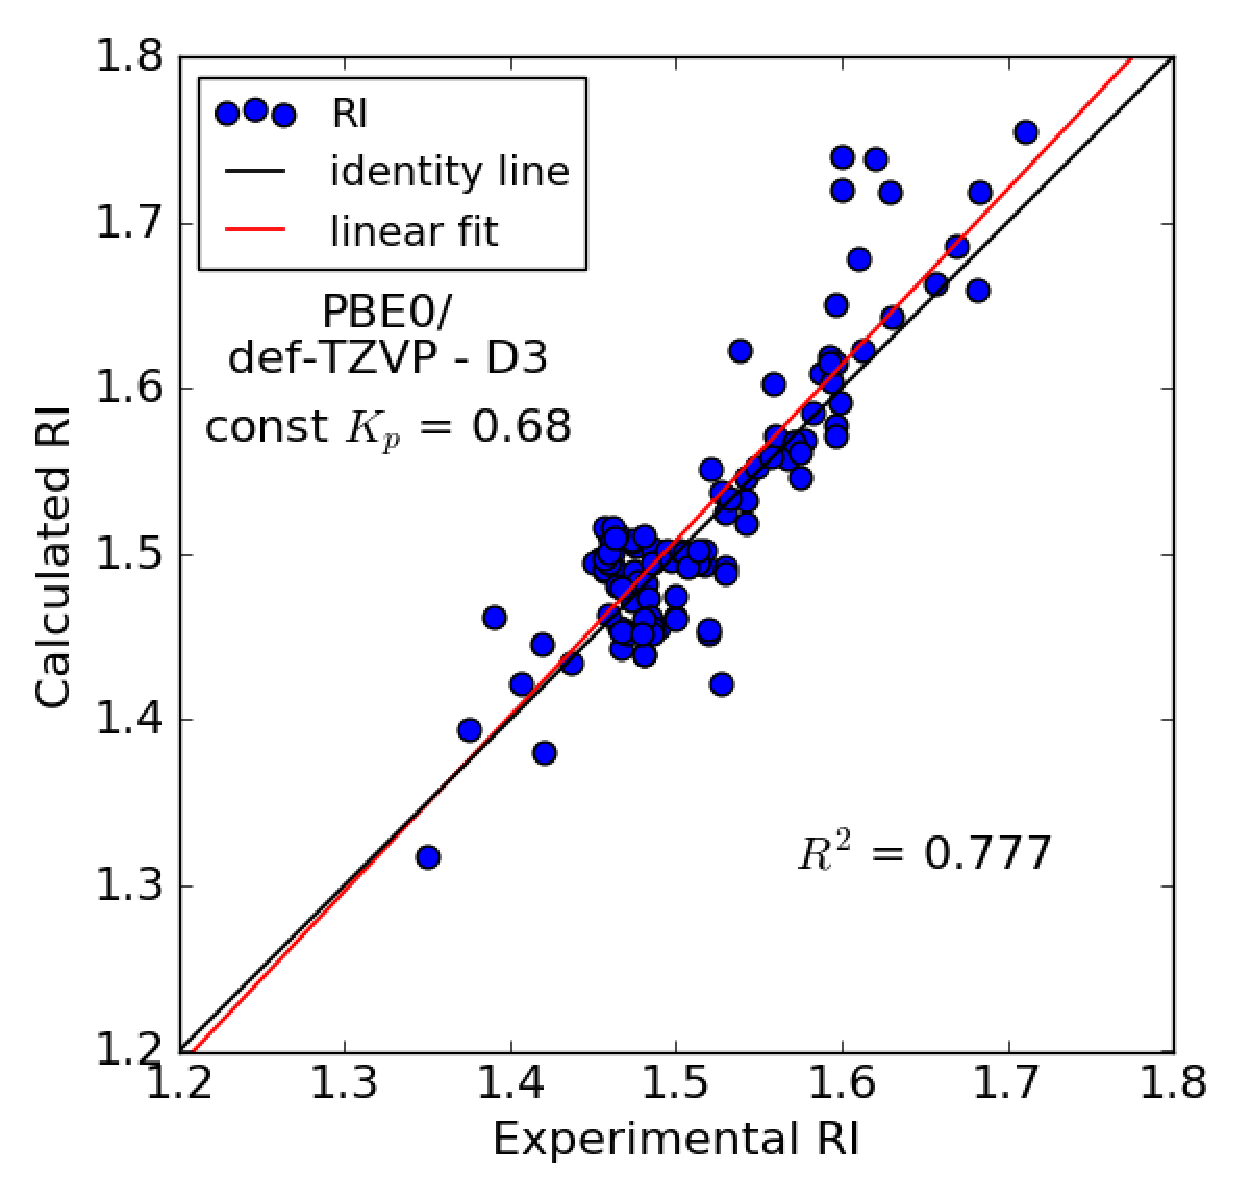
\includegraphics[width=0.6\textwidth]{Chapter-2/Figures/PBE0_Kp_068.eps}
	\caption{Validation of an RI prediction model based on a constant average packing fraction.} 
	\label{fig:validation_const_Kp} 
\end{figure} 

% \textcolor{red}{
The before-mentioned pioneering work by Ramprasad \etal\ offers another instructive reference point. It creates a machine learning prediction model for the dielectric constant ($\epsilon_r = {n_r}^2$) of organic and organometallic compounds that is based on training data from plane-wave DFT for crystalline systems \cite{Huan2016,Sharma2014}. Ramprasad’s database includes 7 experimental data points that can be used for the validation of the underlying DFT model \cite{Mannodi-Kanakkithodi2016}. The DFT predictions show a correlation of only $R^2 = 0.78$ with respect to the experimental data. This suggests that the use of DFT crystal structures may be the cause of some loss in predictive performance, which can propagate into the derived machine learning models. This observation underscores the importance of accurately accounting for the amorphous bulk structure, which our approach achieves. 
% }

% \textcolor{red}{
It is worth stressing that while our discussion focused on non-conjugate polymer examples, our computational protocol can also be employed on conjugate systems provided the extensive regime is considered in the extrapolation schemes. The SVR prediction model for $K_p$ was trained on typical organic polymers and may start to fail for unusual or extreme cases that were not represented in the training set. In such a situation it would be advisable to retrain the model with more targeted training data. 
% }


\subsection{Interplay between Polarizability and Number Density}
\label{subsec:interplay_results}
% Analyze interplay of alpha and N because they are the input slots of the model; do this for our experimental data set
As the Lorentz-Lorenz equation relies on $\alpha$ and $N$ as input parameters, we analyze their interplay for the 112 polymers in our validation and benchmark data set.
% Plot relationship between the polarizability and number density using the values of 112 polymers. 
% Atif: The $\alpha$ and $N$ shown in the relationship plot represent the values for a polymer chain with 50 monomer units.
Fig.\ \ref{fig:relationship} shows the calculated $\alpha$ and $N$ values as well as the contour lines for the resulting RI values in this parameter space. 

\begin{figure}[htbp] 
	\centering
	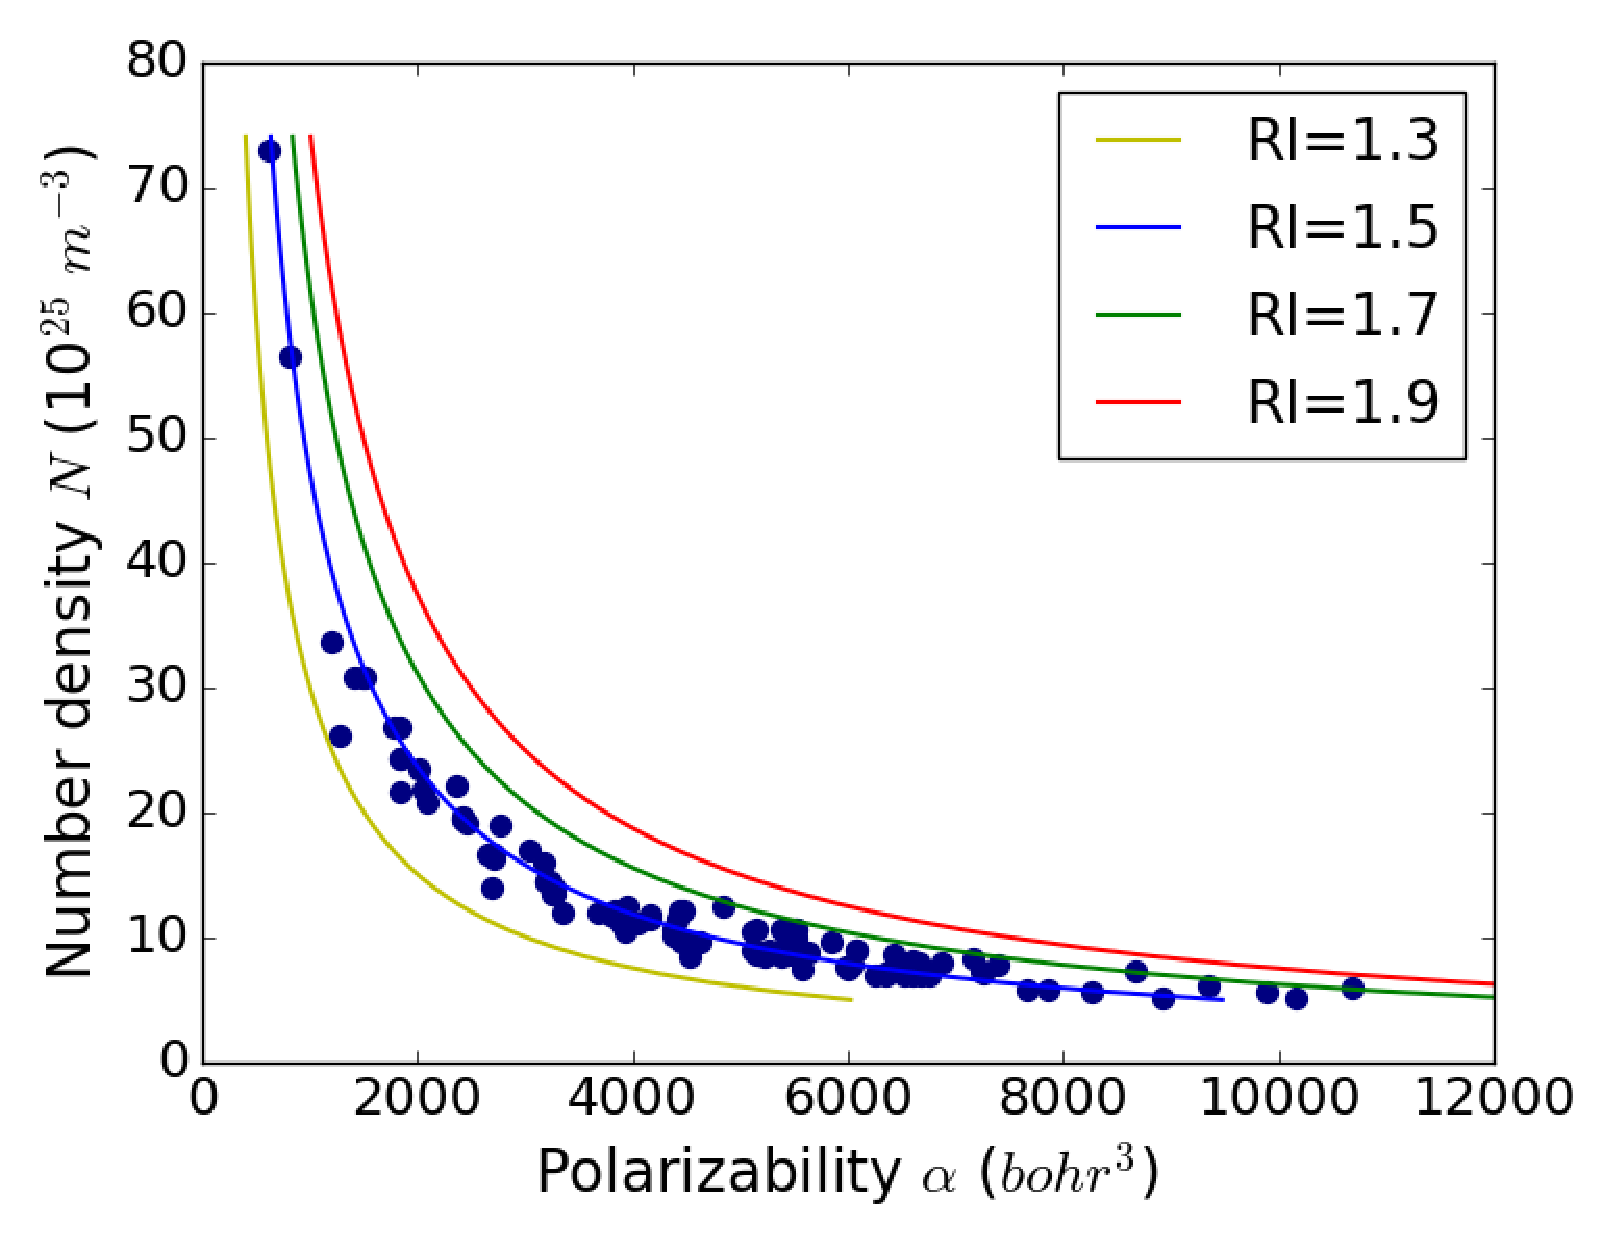
\includegraphics[width=0.6\textwidth]{Chapter-2/Figures/Den_vs_pol_contour.eps}
	\caption{Parameter space of polarizability $\alpha$ and number density $N$ as well as resulting RI value domains with examples from our validation and benchmark data.} 
	\label{fig:relationship} 
\end{figure} 

% Discuss the regions of high RI values and potential pathways of moving towards these regions. Give future directions for the quest of high-RI polymers
To achieve high RI values, a candidate compound must feature both large number density and polarizability values (as is also apparent from the structure of the Lorentz-Lorenz equation). Optimizing both properties simultaneously is a challenging task as extensivity couples $\alpha$ and $N$, \ie  the longer a polymer, the larger $\alpha$ (as $\alpha$ increases with the number of contributing monomer units), but the smaller $N$ (as fewer molecules fit into a given volume element). A design strategy that can be derived from this notion is to incorporate highly polarizable moieties that have a limited effect on the number density. The data set at hand is tilted towards a larger spread in $\alpha$ while $N$ is more clustered. It is worth noting that the RI regions in the $\alpha$ \textit{vs} $N$ parameter space are relatively narrow and most compounds in the data set group around the contour line for RI=1.5. The high-RI examples primarily stand out for large polarizability values rather than large number densities, which supports the before-mentioned design strategy.

% suggests, indicates

% this is basically a repetition of the abstract in rephrased, perhaps more concrete form
\section{Conclusions}
\label{sec:conclusions} 
We have successfully developed a modeling protocol for the accurate prediction of the RI values of organic polymeric materials and validated it against the experimentally known RI values of 112 compounds. The current work is an example for the benefits of fusing physical and data models, with the former providing the general structure of the approach (\ie  the Lorentz-Lorenz equation) and a significant part of the required input parameters (\ie  polarizabilities from \firstprinciples\ quantum chemistry and van der Waals volumes from Slonimskii's method), while the latter provides rapid access to input data that is otherwise not readily available (\ie an SVR model for the packing fraction and an extrapolation scheme for molecular results towards the polymer limit). A subset of our RI protocol can also be used to predict the density of amorphous polymers. Our work is furthermore an example for the great promise of applying machine learning and modern data science in chemical research. In later chapters, we will utilize this new RI protocol to conduct virtual high-throughput screening studies on large-scale candidate libraries with the goal of accelerating the discovery of novel organic materials with unprecedented RI values.

\chapter{Benchmarking DFT Approaches for the Calculation of Polarizability Inputs for Refractive Index Predictions in Organic Polymers}

In chapter 2, we introduced a computational protocol to accurately predict the index of refraction (RI) of organic polymers using a combination of \firstprinciples\ and data modeling. This protocol is based on the Lorentz-Lorenz equation and involves the calculation of static polarizabilities and number densities at the polymer limit. We chose to compute the former within the density functional theory (DFT) framework using the PBE0 functional and def2-TZVP basis set along with D3 dispersion correction. While this choice proved remarkably successful, it is also relatively expensive from a computational perspective and represents the bottleneck step in our RI modeling protocol. It thus limits the utility of the overall approach, in particular in the context of virtual high-throughput screenings of large-scale candidate libraries where efficiency is essential. In the work presented here, we systematically benchmark DFT model chemistries to identify approaches that optimize the balance between accuracy and efficiency for this target application. We compare results for conjugated and non-conjugated polymers, analyze the errors that propagate into the RI predictions, and offer guidance for method selection. 

We thank Prof. Michel Dupuis for helpful discussions on the polarizability calculation of conjugated polymers. 

\section{Introduction}
\label{sec:introduction}
% Address the interest in discovery of high RI polymers
Organic materials with high index of refraction (RI) have gained considerable attention in recent years as they hold tremendous potential for applications in optical and optoelectronic devices \cite{Higashihara2015,Liou2010,Huang2016,Lei2014,Sun2008}. 
However, the vast majority of carbon-based polymers has relatively low RI values (typically in the range of 1.3 to 1.5) \cite{Liu2009,Liu2008c}, which limits their utility.
The discovery and design of compounds with high and very high RIs (greater than 1.8) has thus been an active area of research \cite{Jintoku2014,Griebel2014}. 
The key to increasing the RI values of organic polymers is our ability to tailor their molecular structure 
\cite{Liu2009,Javadi2013,Gazzo2016,Griebel2014}. The number of compounds that results from considering even only a modest collection of building blocks is, however, practically infinite. Experimental efforts are too time-, labor-, and resource-intensive to effectively survey the massive chemical space of this problem setting (and many others in the molecular sciences). 

% Computational HTPS as way out
Computational high-throughput screening studies have emerged as a way to rapidly characterize and assess candidates, and to identify lead compounds for further in-detail investigations.
In the context of optical materials with large dielectric constants (and thus large RI values), the work by Ramprasad and co-workers \cite{Huan2016,Sharma2014,Mannodi-Kanakkithodi2016} is particularly noteworthy.
% Point out the prerequisite for this approach: having a suitable computational protocol for predicting the RI of polymers, i.e., developing this paper is about developing such a protocol
The foundation for \insilico\ screening approaches are suitable modeling protocols for the properties and compound classes of interest. For use in large-scale studies, these protocols not only have to produce sufficiently accurate predictions, but they also have to be fast. 

A number of modeling approaches for the RI values of polymers have been introduced in the past \cite{Huan2016,Sharma2014,Alexandridis2012,Park2011,Redmond2011,Lisa2010,Yu2007a,Holder2006}, each with distinct advantages and disadvantages in the areas of accuracy, reliability, robustness, cost, and range of applicability. 
%Overview of the computational protocol for the prediction of RI of polymers which was developed in previous work.
As discussed in chapter 2, we introduced a new protocol based on a synergistic combination of \firstprinciples\ and data modeling \cite{Afzal2018a}. In this protocol, we calculate RI values using the  Lorentz-Lorenz equation with the number density and polarizability of a given candidate compound as input parameters. We obtain the former using the van der Waals volume and packing factor of the compound, and the latter from quantum chemistry. We compute the van der Waals volumes using Slonimskii's method \cite{Slonimskii1970} and for the packing fraction of the bulk polymer, we introduced a support vector regression \cite{drucker1997,smola2004} (\ie\ machine learning) model. For the polarizabilities, we employ Kohn--Sham density functional theory (DFT) 
% TODO: add Parr/Young and Koch books
with the PBE0/def2-TZVP-D3 model chemistry. We tested the RI predictions of this protocol on 112 non-conjugated polymers and the results show very good agreement with the experimental values ($R^2=0.94$). 
% discuss efficiency
The protocol is overall economical and suitable for high-throughput \insilico\ studies, but the polarizability calculations nonetheless stand out as the bottleneck that limits its efficiency. 

%Importance of benchmarking the polarizability of polymers, both conjugated and non-conjugated polymers. 
In this paper, we present a systematic benchmark study of several DFT model chemistries to identify approaches that deliver a more favorable balance of accuracy and efficiency for polarizabilities in the context of large-scale RI studies. In addition, we demonstrate the performance of extrapolation schemes from small-oligomer calculations to the polymer limit for both conjugated and non-conjugated systems. We provide an analysis of how the errors in the polarizability results propagate into the RI value predictions. 

% TODO: adapt this to this paper
% outline of paper
%In the following section, 
% Sec.\ \ref{sec:methods}
%we introduce the benchmarking methodology and computational details of this study.

% TODO: add stuff here
% the physical foundations of the proposed protocol (Sec.\ \ref{subsec:lorentzlorenz}), 
% motivate a number of assumptions and approximations that are used (Sec.\ \ref{subsec:polarizability} and \ref{subsec:numberdensity}), and discuss the details of the employed computational approach (Sec.\ \ref{subsec:compdetails}). In Sec.\ \ref{sec:results_discussion}, we present and discuss results for the different components (Sec.\ \ref{subsec:polarizability_results}, \ref{subsec:numberdensity_results}, and \ref{subsec:packingfractions_results}) comprising the protocol as well as the overall protocol (Sec.\ \ref{subsec:RI_results}). In each case we evaluate the predictive performance of our model by comparing the obtained results with data from a validation set of experimentally known compounds. Sec.\ \ref{subsec:interplay_results} provides a discussion of the interplay between the physical parameters of our model. 
%Our findings are summarized in Sec.\ \ref{sec:conclusions}.



\section{Background and Methods}
\label{sec:methods}

\subsection{Benchmarking Setup}
\label{subsec:benchmarking}
% recap how protocol works and how we compute the polarizabilities
As mentioned before, our RI protocol introduced in Ref.\ \cite{Afzal2018a}, employs the PBE0 hybrid functional \cite{Adamo1999}, atom-centered def2-TZVP basis set \cite{Weigend2005}, and D3 dispersion correction \cite{Grimme2010} for the closed-shell, all-electron calculation of the static polarizabilities that serve as input for the Lorentz--Lorenz equation. The target systems are amorphous, quasi-infinite polymers, and we obtain the polarizability results at the polymer limit through an extrapolation scheme from a sequence of small-oligomer calculations. This scheme is based on the finite correlation length in these systems, which typically leads to an early onset of extensivity in the response properties. 
% Once the polarizability increase per number of monomer units has reached a constant value     

% comparison of polarizabilities to reference DFT
In this study, we benchmark the accuracy of several DFT functionals and basis sets. As a reference, we chose the double hybrid functional B2PLYP \cite{Grimme2006} and def2-TZVP basis set. 
% comparison of RI to experimental data
The calculated RI values from different methods are compared with the experimental RI values of 112 polymers.

% Further, this study will give guidelines regarding the selection of methods for calculating polarizability and RI of polymers. 
%Demonstrate how benchmarking will lead to an efficient large scale virtual high throughput screening.
% Based on the benchmarking results, appropriate methods can be selected to be used in the RI prediction protocol, which could be potentially used in automated high-throughput framework. Thus, the results from this work will lead to an efficient large scale virtual high throughput screening of potential high RI polymer candidates.





% explain method used, summarize previous paper sections on polarizability
% oligomers to polymer limit    

%Refer the protocol to determine the polarizability of polymers from RI protocol paper.

Extrapolation schemes for both conjugate and non-conjugated polymers are presented in this work. 
% Explain the polymers selected as an example for non-conjugated and conjugated polymers.
For non-conjugated polymers, polyethylene (PE) is selected as an example polymer, whereas for conjugated polymers, polyacetylene (PA) is selected. For comparison between conjugated and non-conjugated polymers, two polymers polythiophene (PT) and poly(1,4-phenylene) (PB) are selected as examples. The conjugation of these polymers is broken by introducing non-planarity in the polymer chain. Non-planar chains are obtained by constraining consecutive rings perpendicular to each other (see fig.\ \ref{fig:PB_PT_structure}).

\begin{figure}[htbp] 
	\centering
	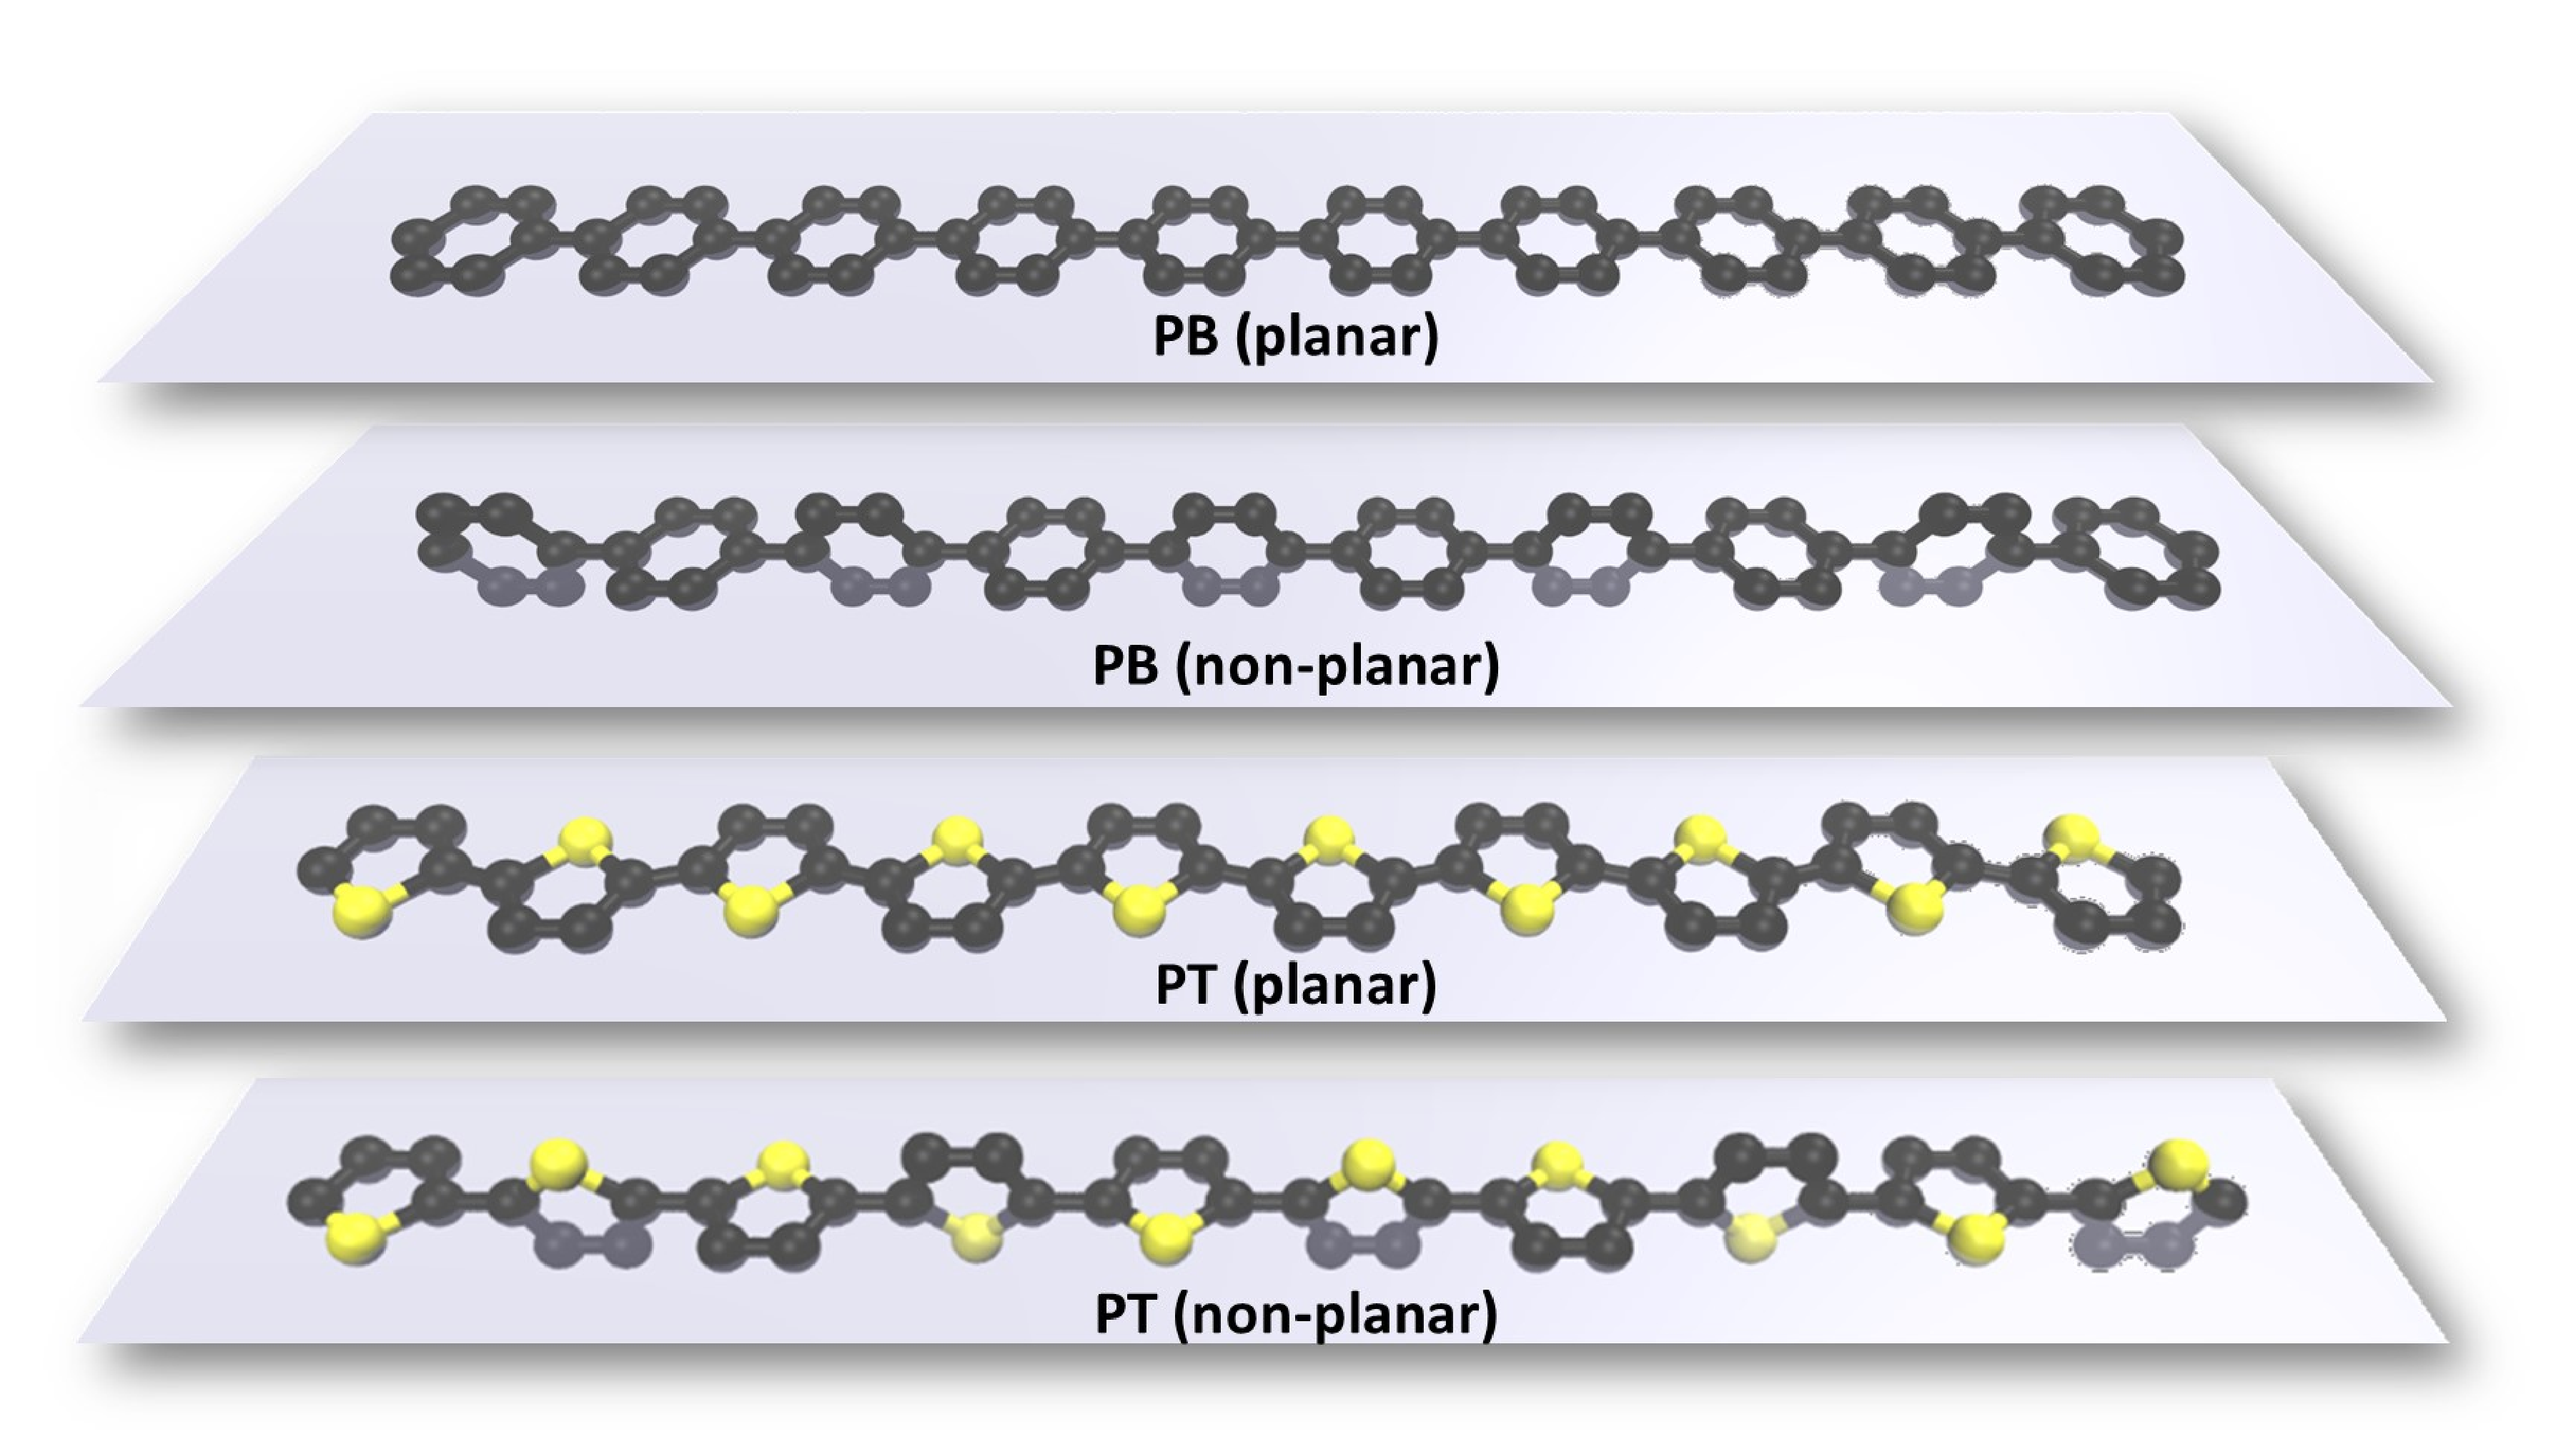
\includegraphics[width=0.744\textwidth]{Chapter-3/Figures/PB_PT_structure.eps}
	\caption{Representation of planar/non-planar structures of PB and PT with a chain length of 10.} 
	\label{fig:PB_PT_structure} 
\end{figure}  

% TODO: get citations from previous papers

%Explain briefly different methods used for benchmarking the polarizability of polymers.
The values of polarizability are generally dependent on DFT approximation and different model chemistries will give different results. In our previous work, we used PBE0/def2-TZVP to calculate polarizability of polymers, but a benchmarking study is necessary to determine a more rational method towards polarizability calculation. Therefore, in this study, polarizability of the polymers is calculated using six different functionals including BP86, PBE0, TPSSh, M06-2X, B2PLYP, and B3LYP. Each of these functionals was used with two def2 basis sets by the Karlsruhe group \cite{Weigend2005}, def2-SVP and def2-TZVP, which are abbreviated as DZ and TZ respectively. Geometry optimization of oligomers is performed at B3LYP/DZ. All the single point calculations as well as the geometry optimizations were performed with D3 correction \cite{Grimme2010}. All the quantum computations are performed using the ORCA quantum chemistry package \cite{Neese2012}.

%Explain the RI model developed for polymers. Lorentz-Lorentz equation and the machine learning model for packing fraction.
The RI of polymers is calculated based on the Lorentz-Lorenz equation, which includes the calculation of two different properties, polarizability and number density. The former is calculated by the method mentioned above, whereas the latter is calculated based on van der Waals volume and packing fraction. The van der Waals volume of the molecules is calculated using Slonimskii's methods \cite{Slonimskii1970}. However, the critical parameter in number density calculation is the packing fraction of the bulk polymer. The most efficient way of calculating packing fraction is to perform molecular dynamics study, but this approach is computationally expensive, therefore, not a viable option for high-throughput screening studies. In our RI prediction model, we established a machine learning approach using a support vector machine on a training data set compiled from the literature to correlate the polymer structure with their packing fraction. The same method is also used in this work for RI calculation.

%Validating the calculated results using 112 experimental values.
The RI values from different model chemistries is validated by comparing with experimental RI values of 112 polymers. The experimental values of these polymers have been taken from Bicerano, polymerdatabase.com, chemicalbook.com, and scientificpolymer.com \cite{Bicerano2002}. 

%Describe the tools for automating the framework of RI calculation of polymers.
In this work, 112 polymers polarizability values are calculated using 12 different methods. For each polymer, four individual calculations are performed from monomer to tetramer. This leads to a total of 5376 calculations. We performed all these calculations in an automated fashion using \chemhtps. 

%Describe the terminology used for error analysis.
The following abbreviations are used for error analysis terms:
MAPE (mean absolute percentage error),
RMSE (root mean squared deviation),
AE (average error),
MaxE (maximum error),
SPRE (difference of maximum and minimum error),
MAE (mean absolute error),
MARE (mean absolute relative error) and
RMSRE (root mean squared relative error)


\section{Results and Discussion}
\label{sec:results_discussion}

%Polarizability of non-conjugated polymer, polyethylene, comparison of different method for the variation of polarizability with the chain length. Fit to a linear regression model and discuss the trends seen.
In our previous studies, we showed that the polarizability of non-conjugated polymers, calculated at PBE0/TZ level, varies linearly with increasing chain length. Here, we calculate the polarizabilities of polyethylene (PE) using different methods. The plot in fig:\ \ref{fig:PE_per} shows the comparison between different methods. Blue color is for DZ and red for TZ. 

Observations:

i. In all methods, the polarizability values have a linear relationship with the PE oligomer chain length. The initial decrease in the values from monomer to trimer is due to the end effects of the hydrogen.

ii. The polarizability per oligomer of PE converge to a constant value right after trimer. This suggests that for non-conjugated systems, it is sufficient to calculate polarizability until tetramer. 

iii. The calculated polarizability values in the decreasing order of BP86\ $>$ B3LYP\ $>$ TPSSh\ $>$ PBE0\ $>$ M06-2X\ $>$ B2PLYP

It is well known that LGA and GGA functionals significantly overestimate the polarizability values, which is also depicted in these studies. The key to solve the problem of overestimation is to include an exact exchange treatment \cite{Mori-Sanchez2003}. Therefore, the functionals  B3LYP, TPSSh, PBE0 and M06-2X, which include HF treatment predict lower polarizability values. Further, the functionals which include perturbation theory along with HF, \eg\ double hybrid functional B2PLYP, predict much lower polarizability values. 
This benchmarking study will assist in understanding the degree of over-prediction for various lower level methods.

\begin{figure}[htbp] 
	\centering
	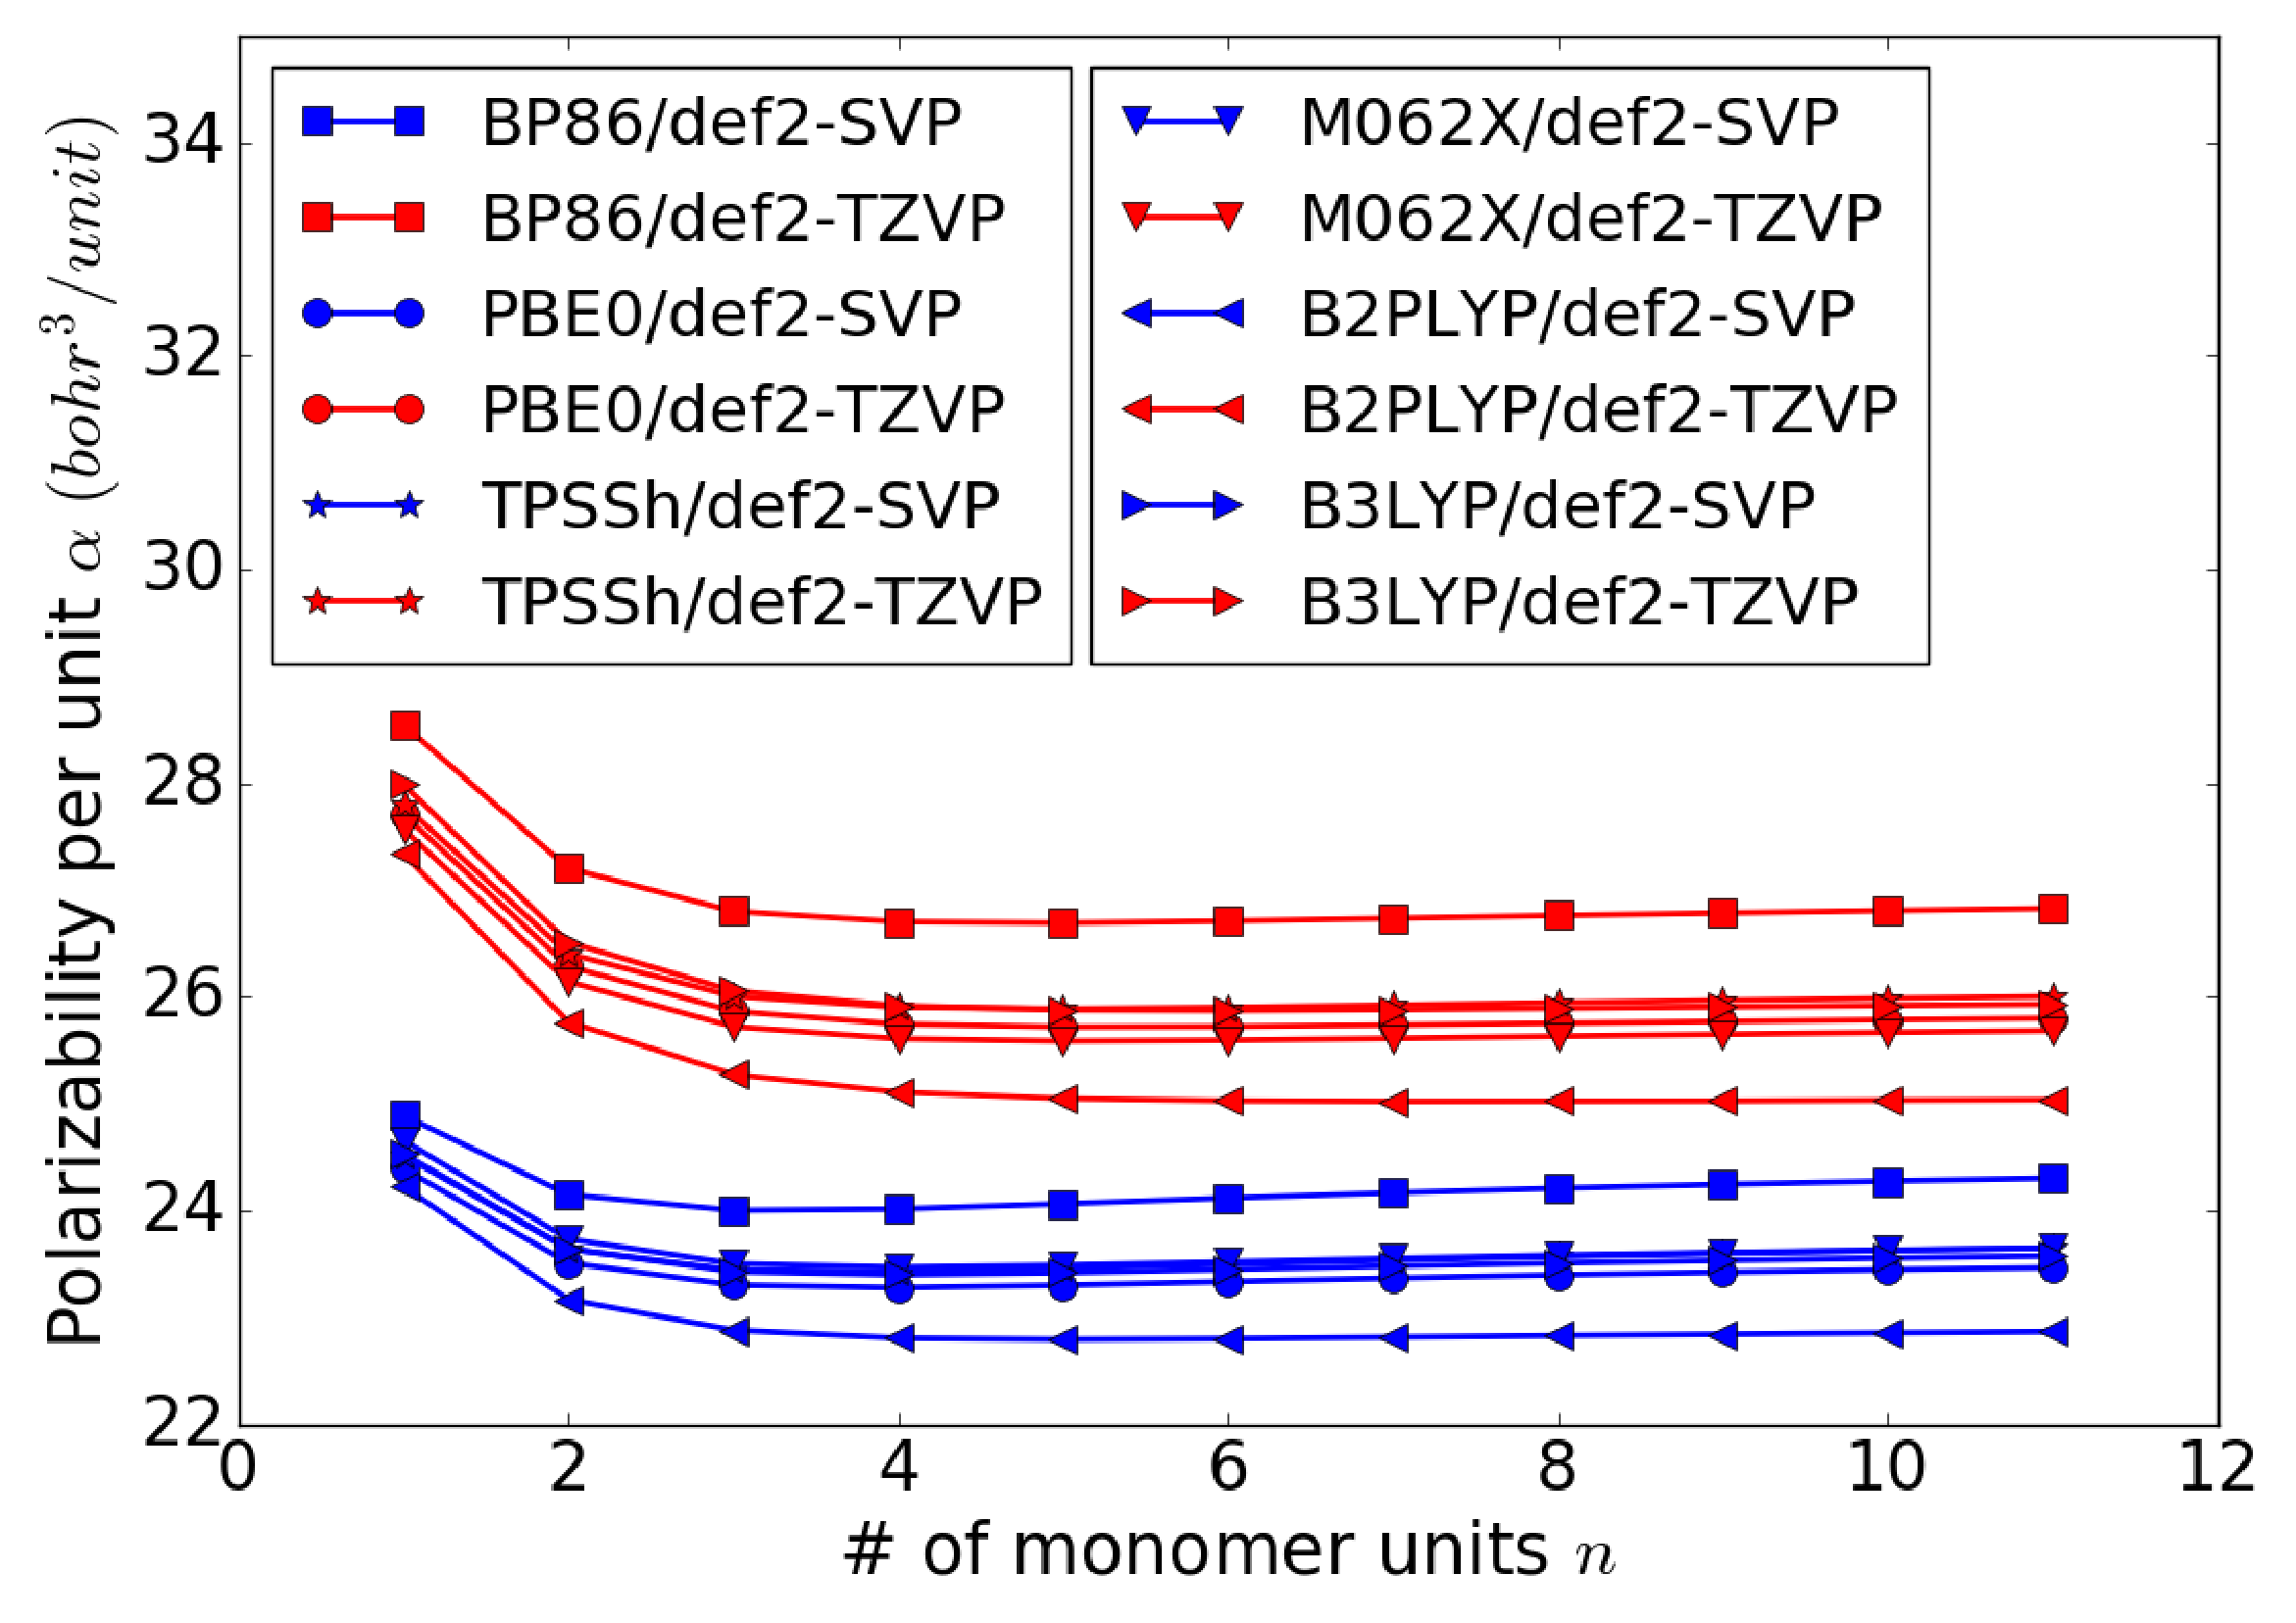
\includegraphics[width=0.744\textwidth]{Chapter-3/Figures/PE_per.eps}
	\caption{Polarizability per oligomer unit of polyethylene with varying chain length calculated from different model chemistries.} 
	\label{fig:PE_per} 
\end{figure}  

%Repeat the above part for conjugated polymer, polyacytylene. 
For conjugated polymers, polyacetylene (PA) is selected as test polymer. Polarizability with increasing chain length is calculated using different functionals and basis set (see fig:\ \ref{fig:PA_per}). The variation of polarizability follows a non-linear behavior with the increasing oligomer length. This is because, as the length is increasing, the conjugation in the molecule also increases leading to increased polarizability. Non-linear correlation can be used to fit the polarizability variation of conjugated polymers. 

\begin{figure}[htbp] 
	\centering
	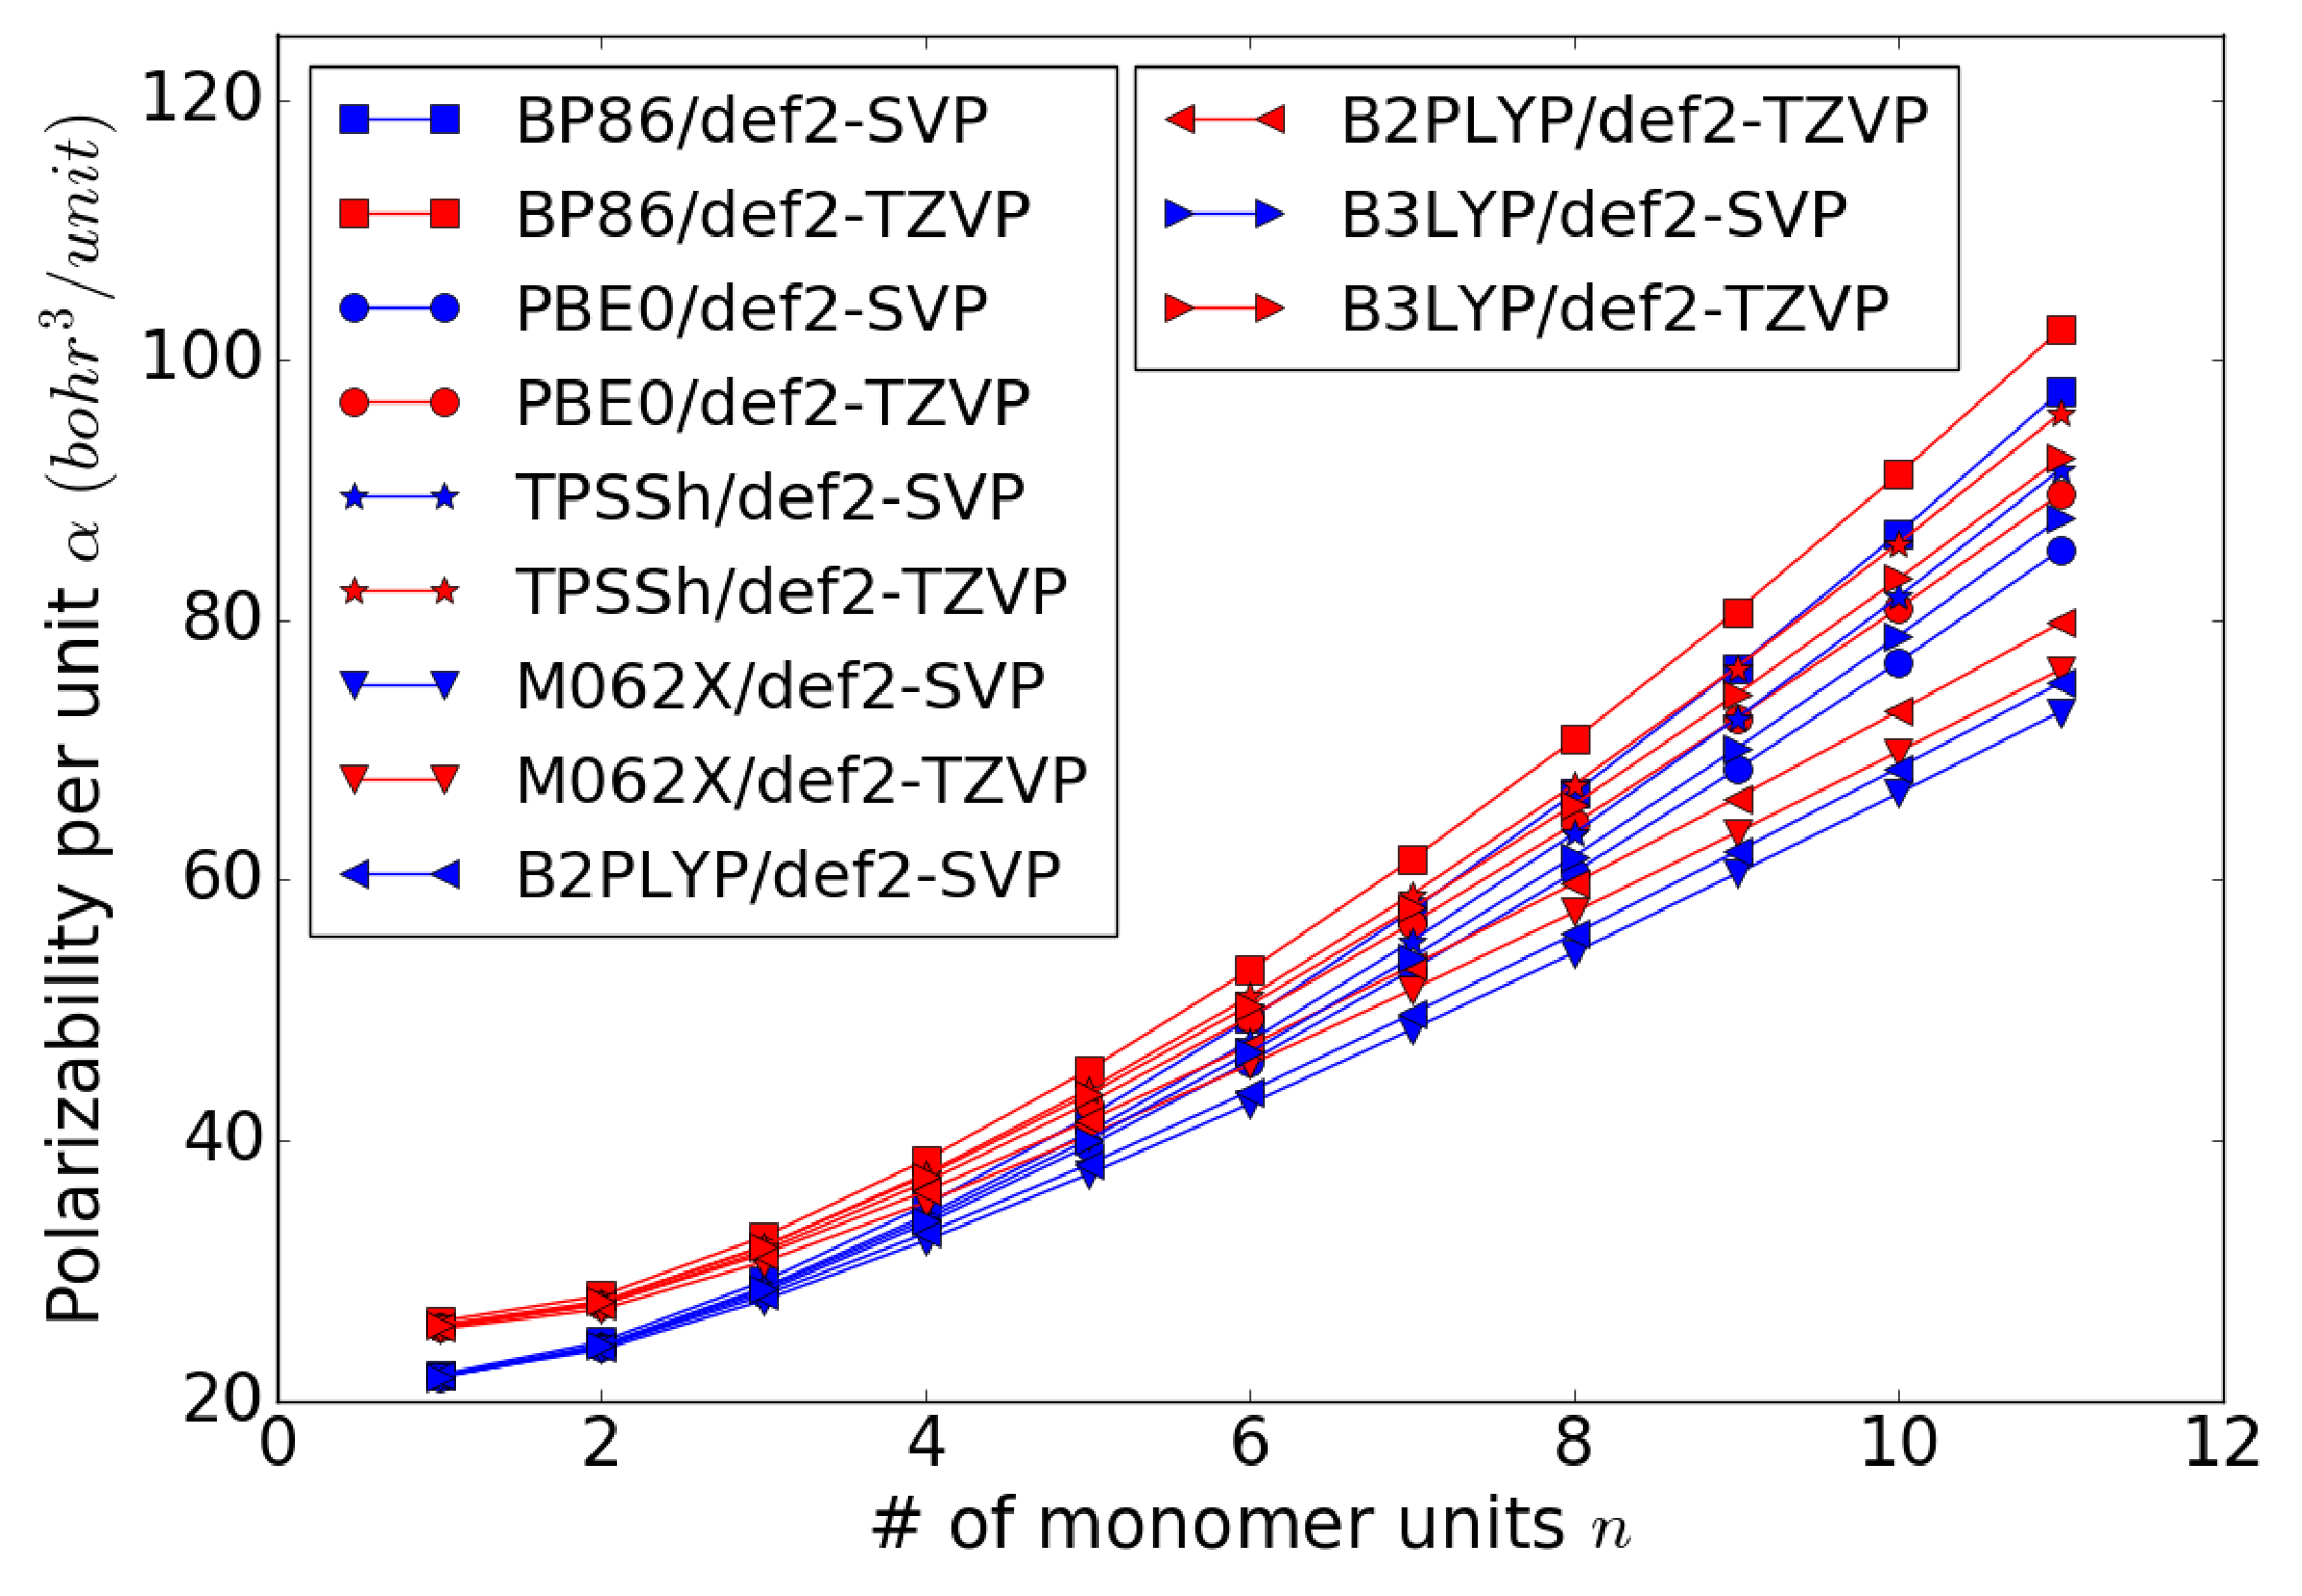
\includegraphics[width=0.744\textwidth]{Chapter-3/Figures/PA_per.eps}
	\caption{Polarizability per oligomer unit of polyacetylene with varying chain length calculated from different model chemistries.} 
	\label{fig:PA_per} 
\end{figure}  

%Comparison of polarizability results when the conjugation is broken by introducing an aliphatic carbon in between. Can also break the conjugation by making non planar molecules.

A better way to compare conjugated and non-conjugated polymers is to break the conjugation by introducing an aliphatic carbon between aromatic rings. For this, two conjugated polymers, PT and PB, are selected and conjugation is broken by introducing non-planarity in the molecule as shown in fig:\ \ref{fig:PB_PT_structure}. The polarizability per oligomer unit increases with chain length for planar PB and PT polymers (see fig:\ fig:\ \ref{fig:C_NC_PB} and fig:\ \ref{fig:C_NC_PT}). For the non-planar PT and PB, the increase in polarizability per oligomer is significantly less. This suggests that the conjugation plays an important role in the polarizability of the polymers. The slight increase of polarizability in non-planar PT and PB shows that there exists a weak conjugation between the aromatic rings. This observation can be better understood by looking at the HOMO and LUMO of PT and PB with a chain length of 5 (see fig:\ \ref{fig:PB_PT_HOMO_LUMO}). The HOMO for planar PB and PT is alternating, suggesting a strong conjugation in the molecule, whereas for non-planar PB and PT, the HOMO is slightly alternating which shows evidence of a weak conjugation. The LUMO distribution of planar PB and PT extends along the full length of molecule, suggesting that the excited electrons would have a clear path to flow. 

\begin{figure}[htbp] 
	\centering
	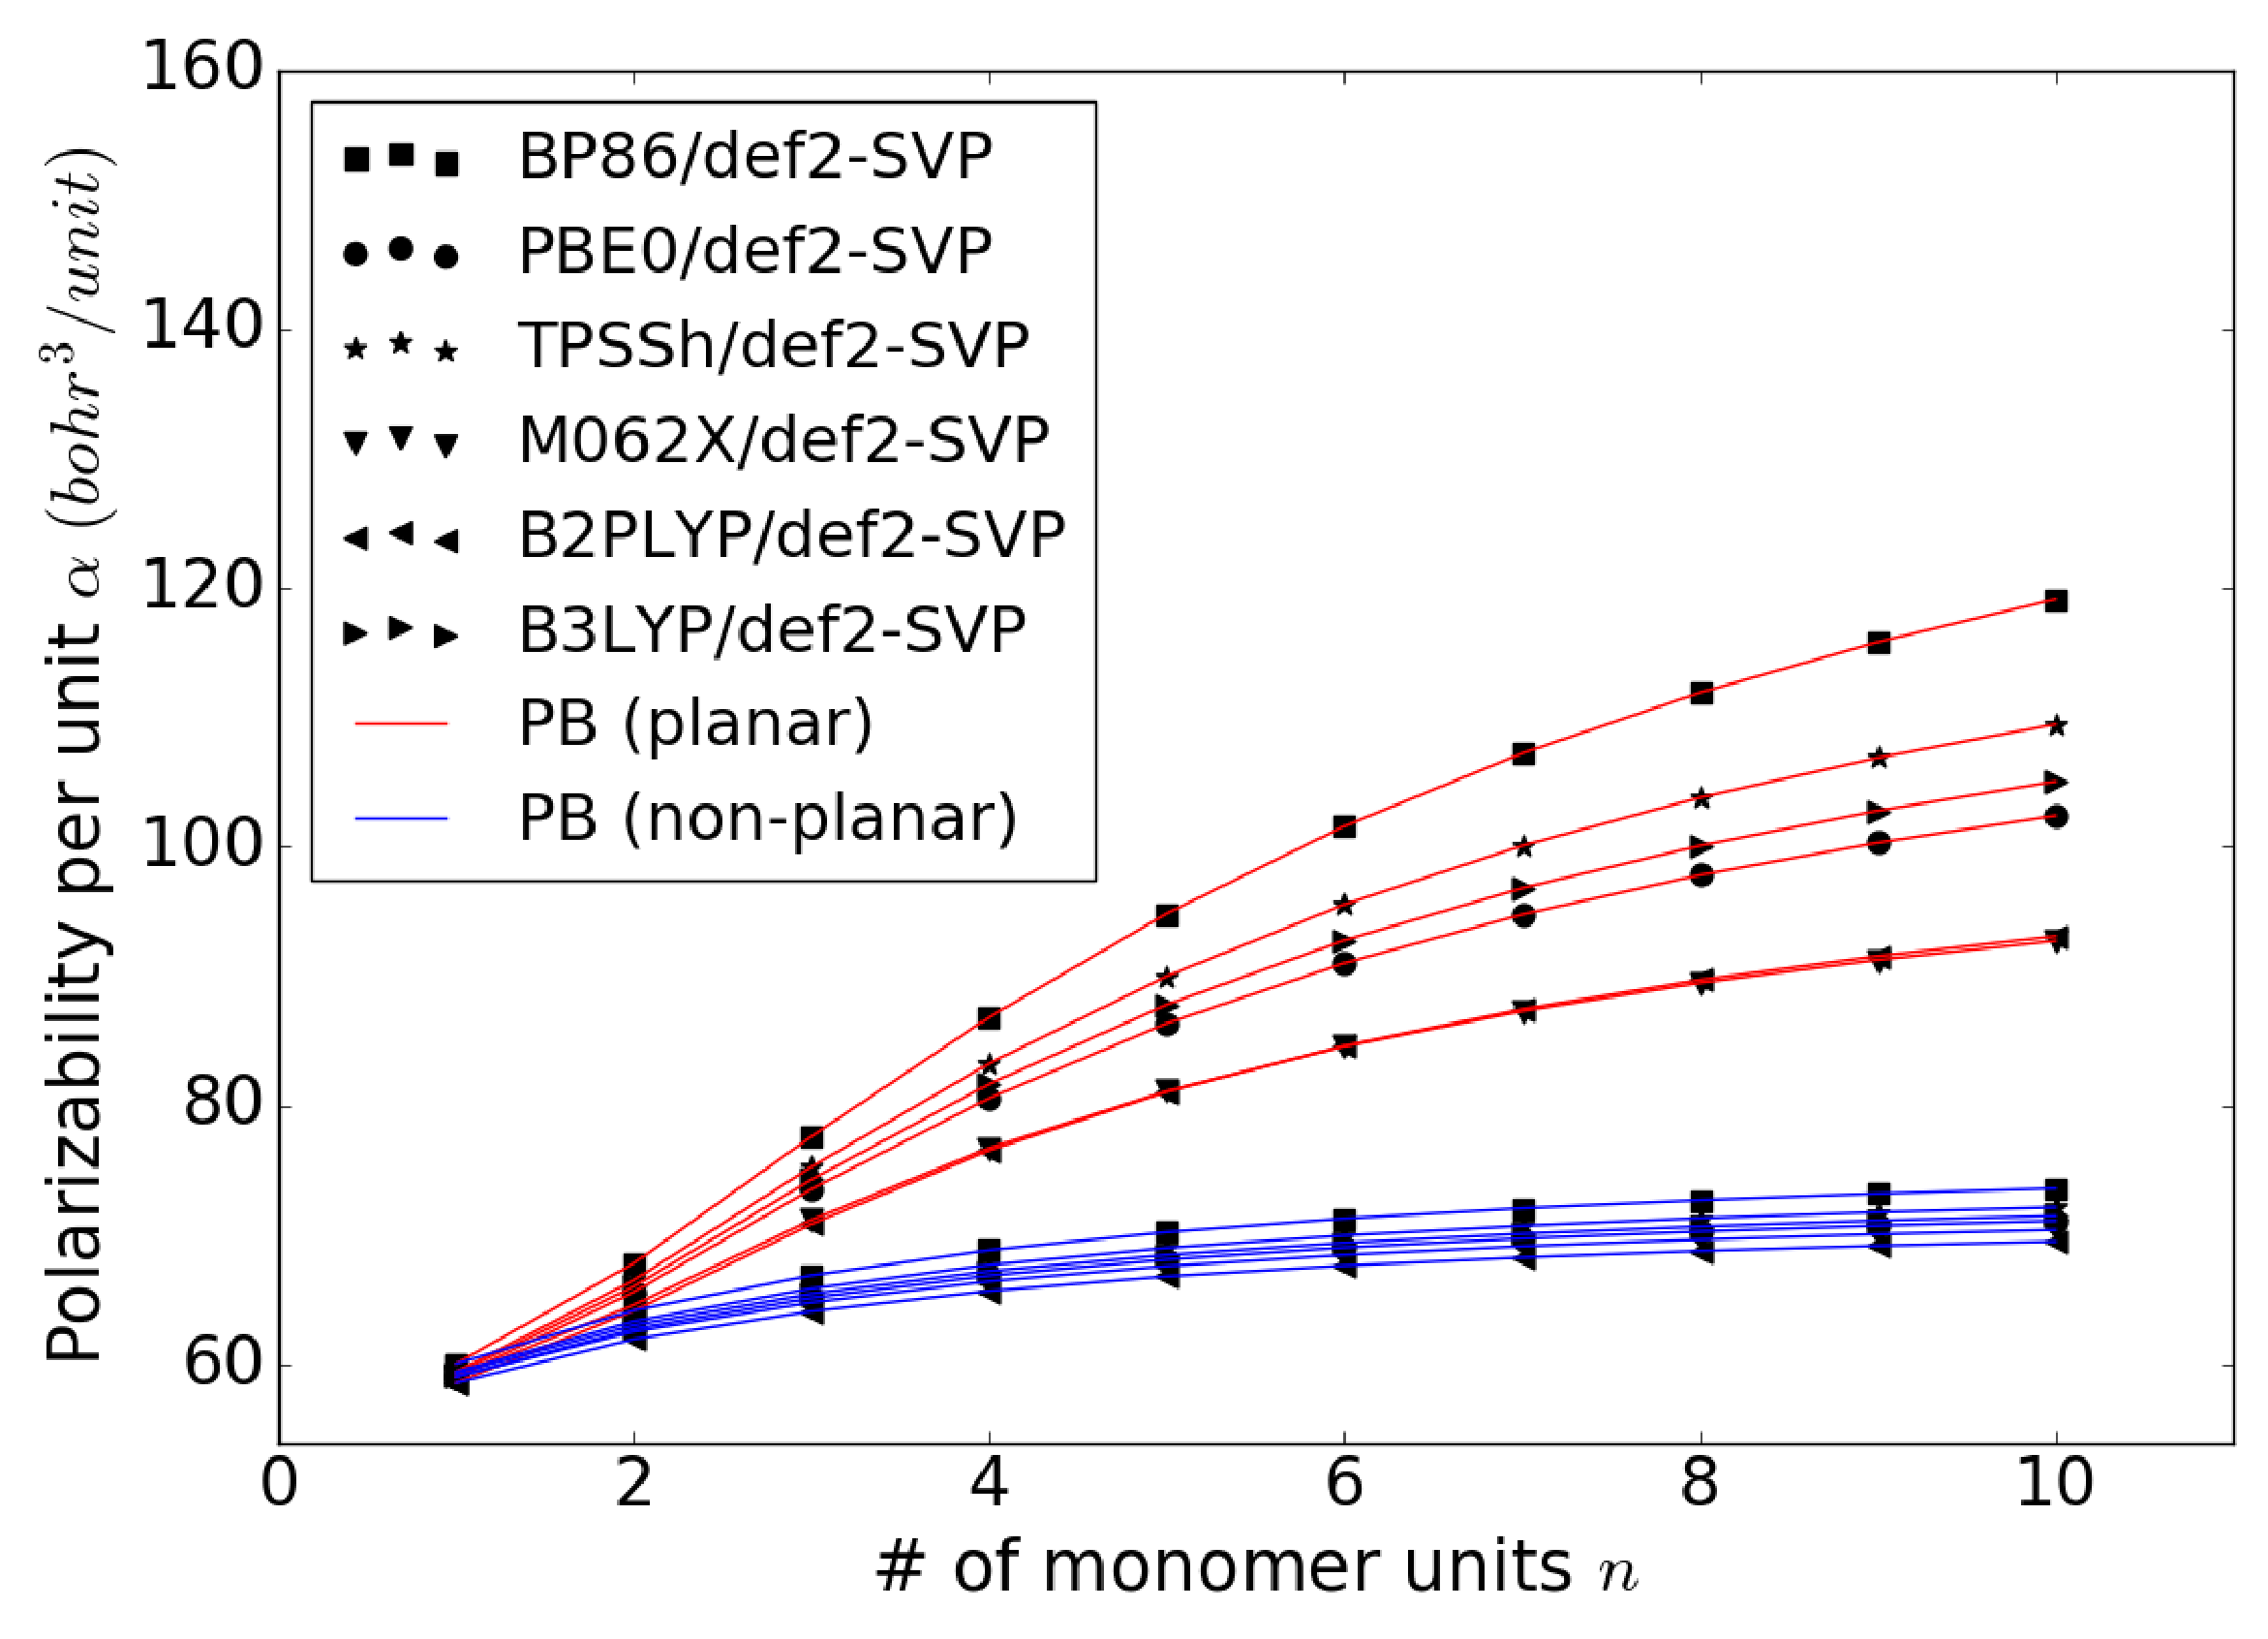
\includegraphics[width=0.744\textwidth]{Chapter-3/Figures/C_NC_PB.eps}
	\caption{Polarizability per oligomer unit of planar and non-planar poly(1,4-phenylene) (PB) with varying chain length calculated from different model chemistries.} 
	\label{fig:C_NC_PB} 
\end{figure}  

\begin{figure}[htbp] 
	\centering
	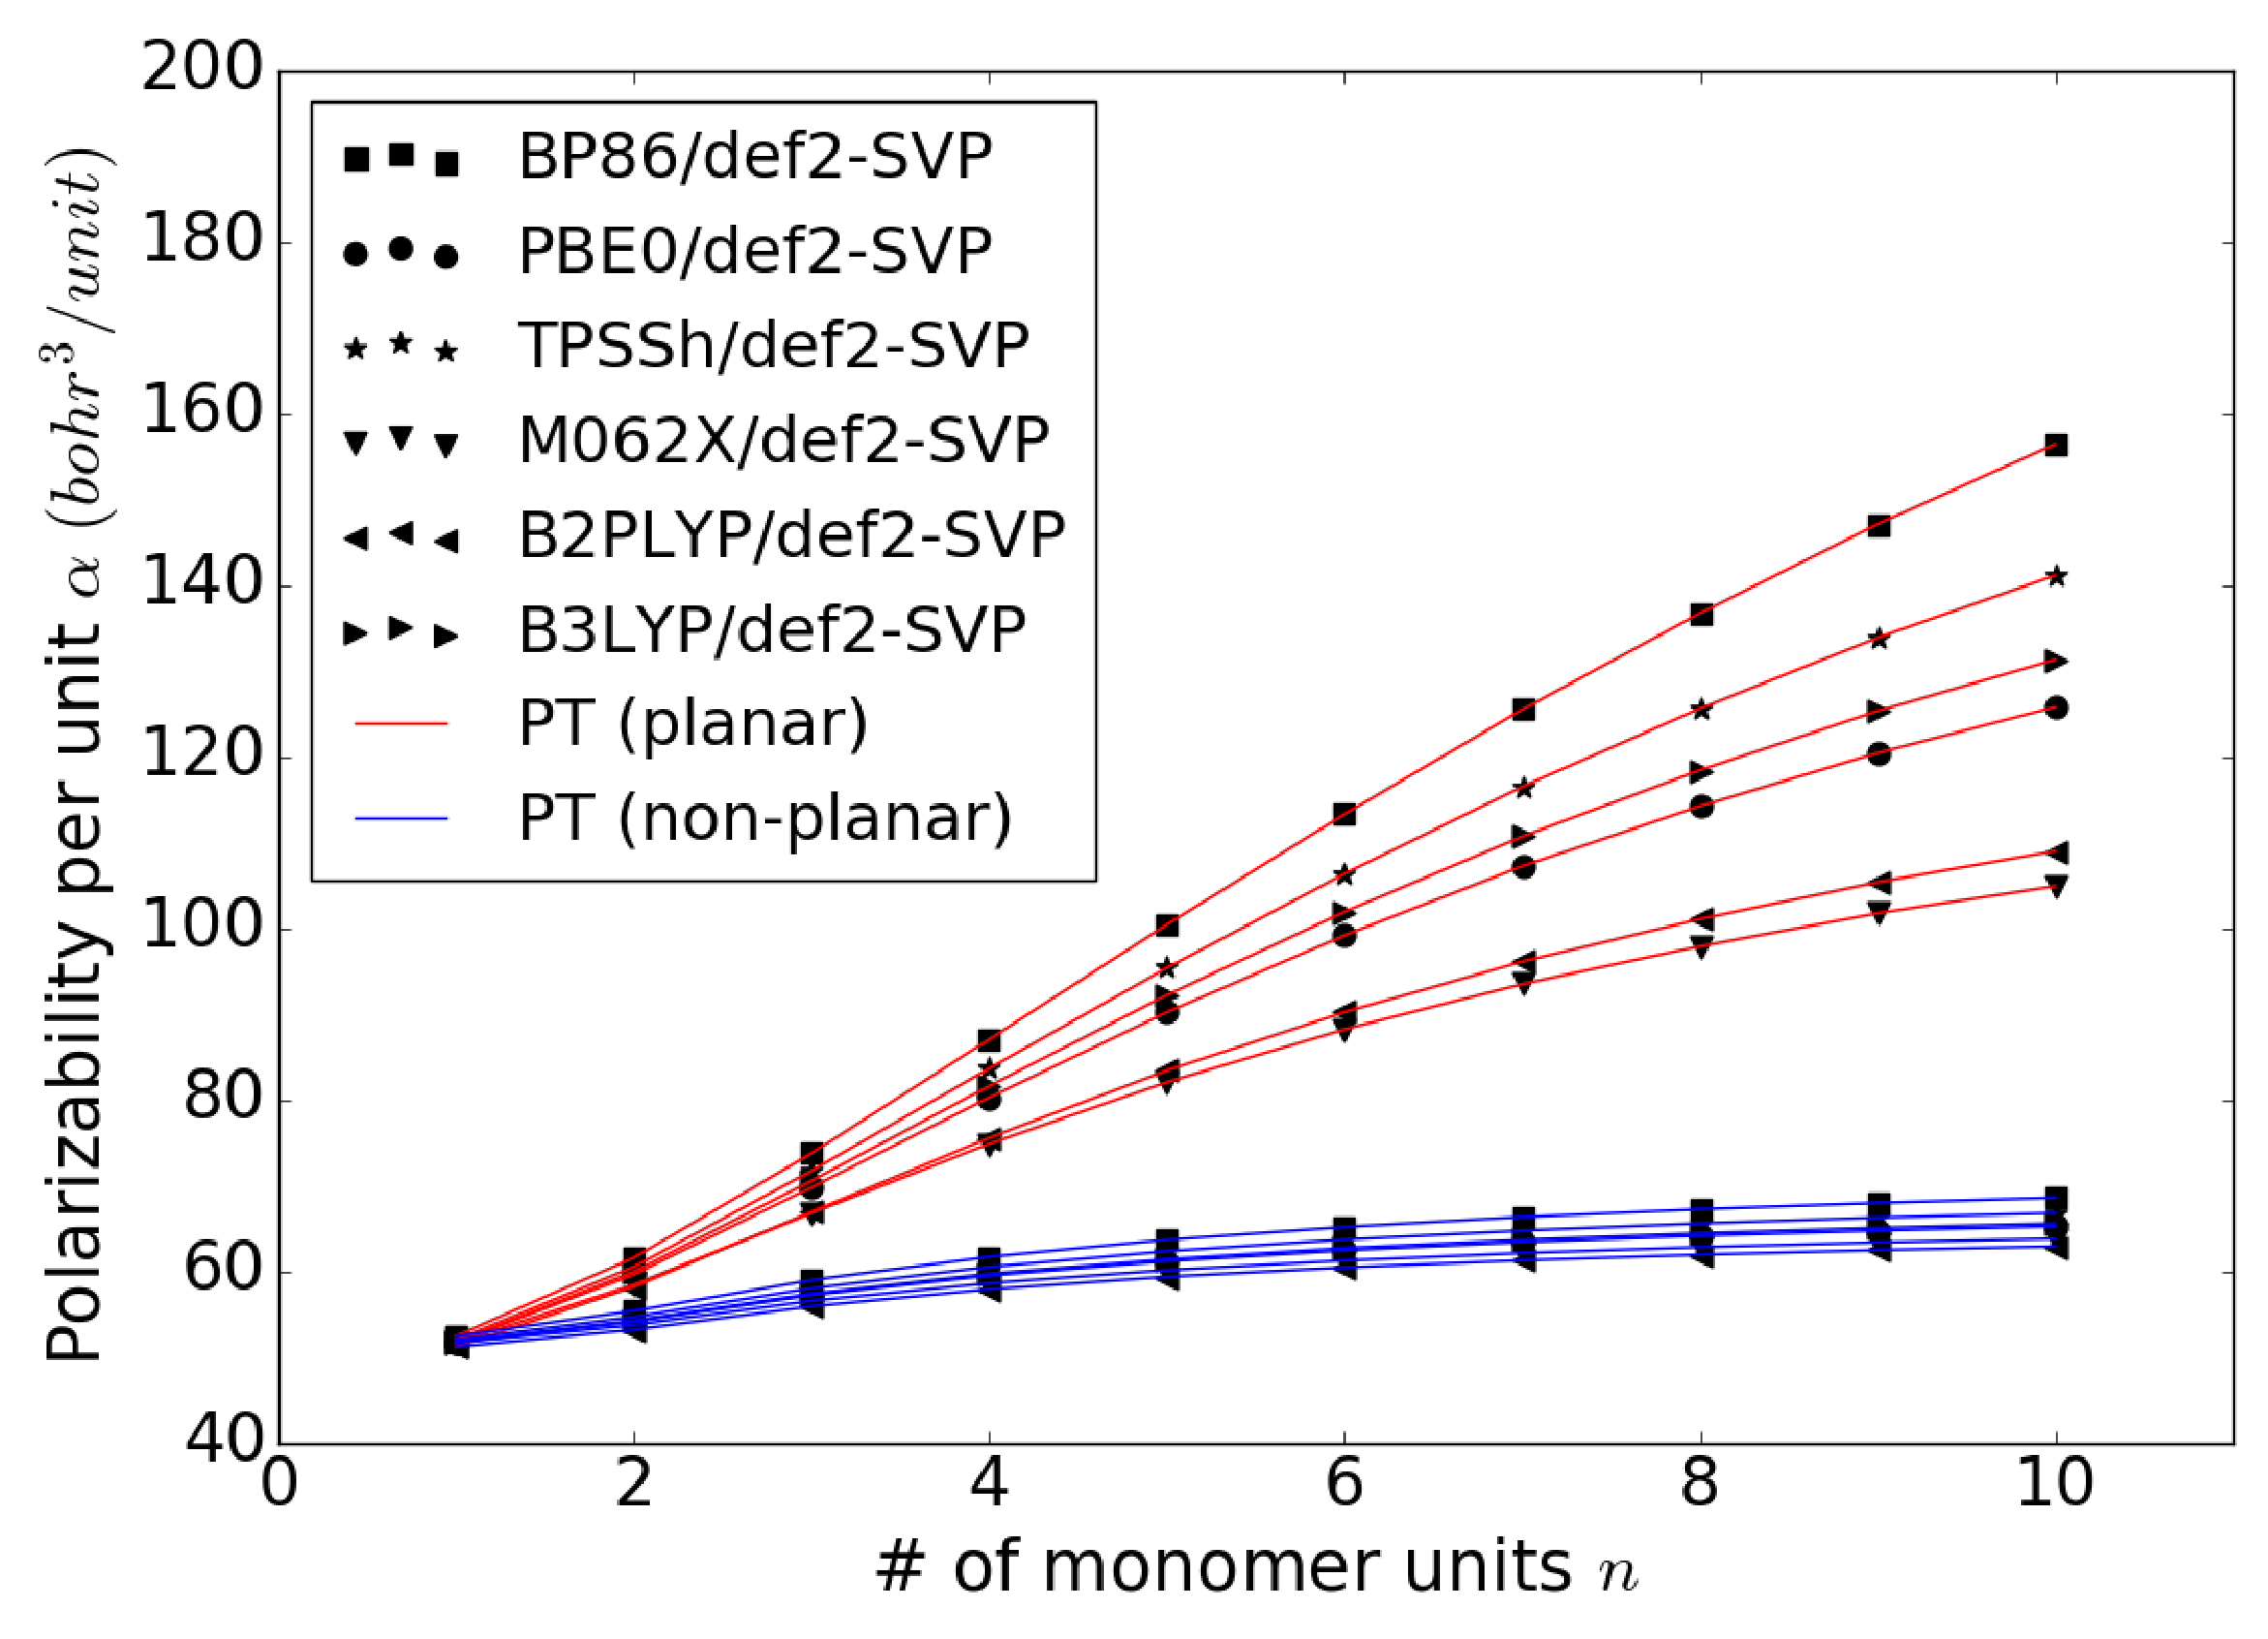
\includegraphics[width=0.744\textwidth]{Chapter-3/Figures/C_NC_PT.eps}
	\caption{Polarizability per oligomer unit of planar and non-planar polythiophene (PT) with varying chain length calculated from different model chemistries.} 
	\label{fig:C_NC_PT} 
\end{figure}  

\begin{figure}[htbp] 
	\centering
	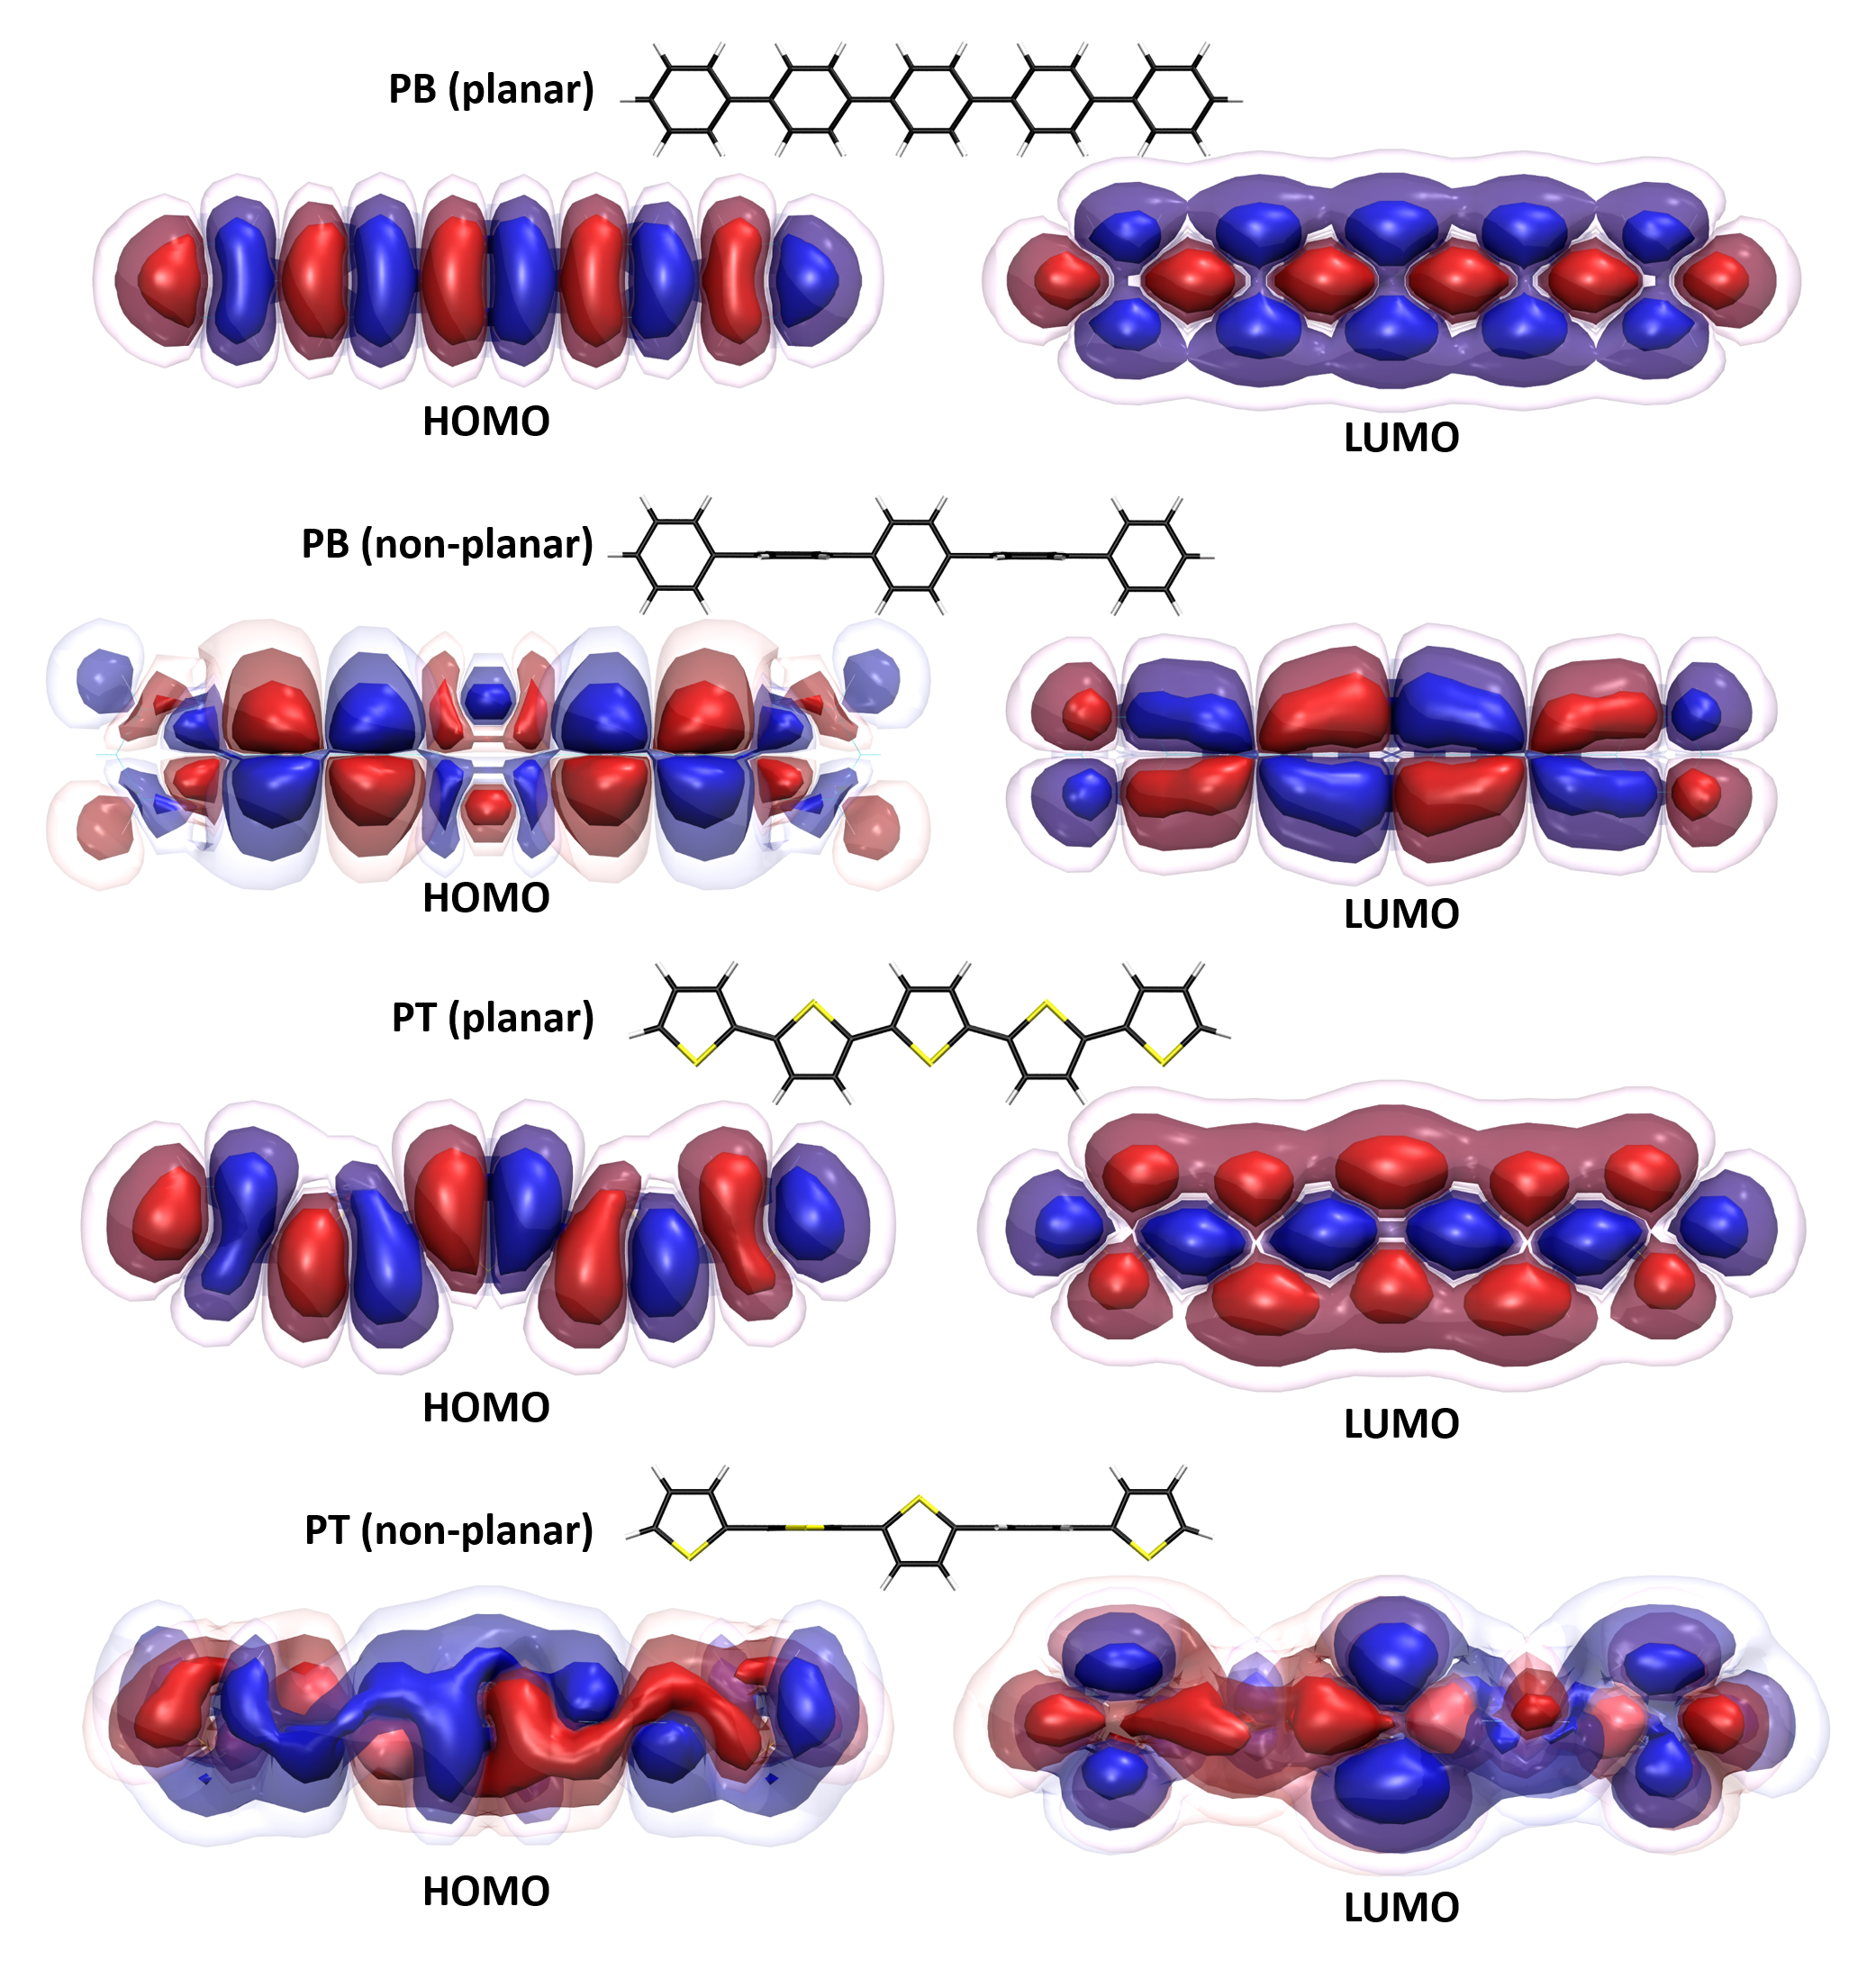
\includegraphics[width=0.744\textwidth]{Chapter-3/Figures/PB_PT_HOMO_LUMO.eps}
	\caption{HOMO (B2PLYP/TZ) and LUMO (B2PLYP/TZ) of planar/non-planar poly(1,4-phenylene) (PB) and polythiophene (PT).} 
	\label{fig:PB_PT_HOMO_LUMO} 
\end{figure}  

%Extrapolation scheme for conjugated polymers. Fit the model to a non-linear equation similar to the equation in Prof. Dupuis paper. Also, find trends.
The variation of polarizability per oligomer unit for conjugated polymers initially increases linearly and then asymptotically converges. A mathematical expression was proposed in literature as shown in the eqn:\ \ref{eqn:1} \cite{Hurst1988}. However, this expression does not fit well for long oligomers (see fig:\ \ref{fig:Pol_fit_all_PBE0_TZ_old}). An extra term is added to the expression as shown in eq:\ \ref{eqn:2}, such that the variation fits well for longer chains (see fig:\ \ref{fig:Pol_fit_all_PBE0_TZ}). This expression is valid for all the three studied conjugated polymers PA, PB and PT. Thus, using this expression, the polarizability of polymer limit can be calculated based on the calculations for small chain oligomers. 

\begin{equation} \label{eqn:1}
\log(\alpha)=a+\frac{b}{N}+\frac{c}{N^2}
\end{equation}


\begin{figure}[htbp] 
	\centering
	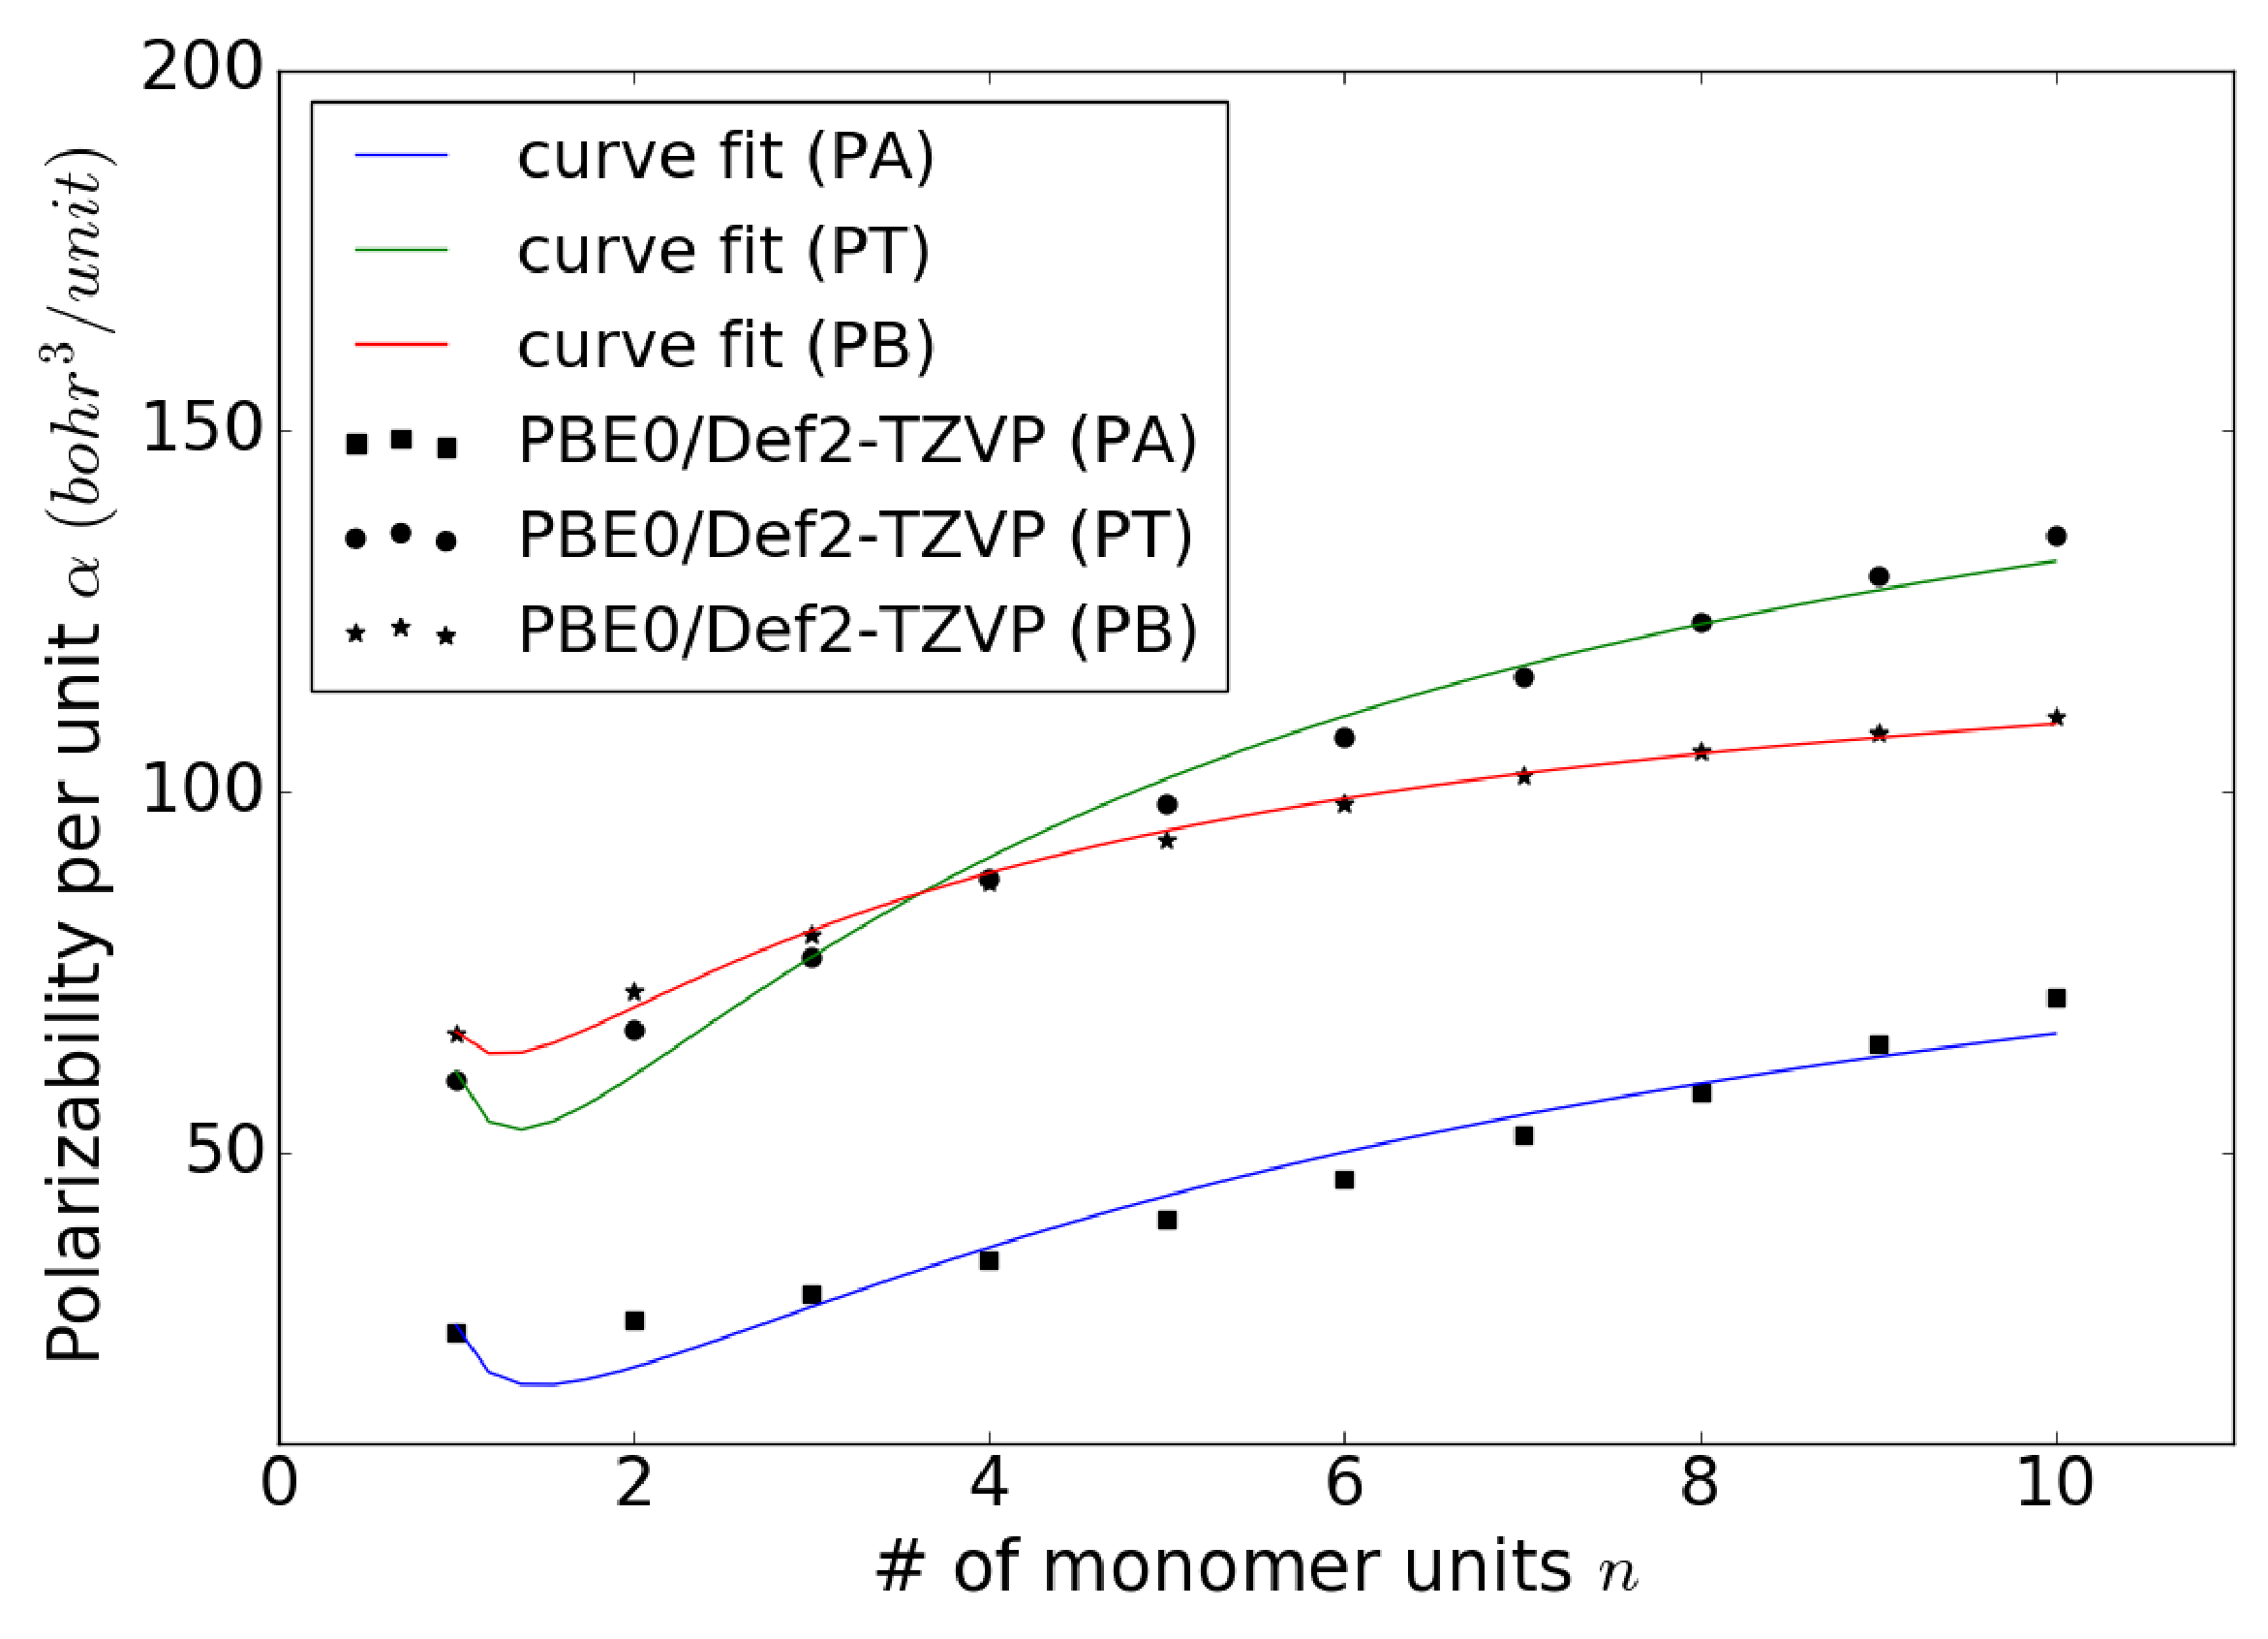
\includegraphics[width=0.744\textwidth]{Chapter-3/Figures/Pol_fit_all_PBE0_TZ_old.eps}
	\caption{Curve fitting using polarizability expression from \cite{Hurst1988} for the conjugated polymers polyacetylene (PA), poly(1,4-phenylene) (PB) and polythiophene (PT). Polarizability is calculated using PBE0/TZ.} 
	\label{fig:Pol_fit_all_PBE0_TZ_old} 
\end{figure}  


\begin{equation} \label{eqn:2}
\log(\alpha)=a+\frac{b}{N}+\frac{c}{N^2}+\frac{d}{N^3}
\end{equation}


\begin{figure}[htbp] 
	\centering
	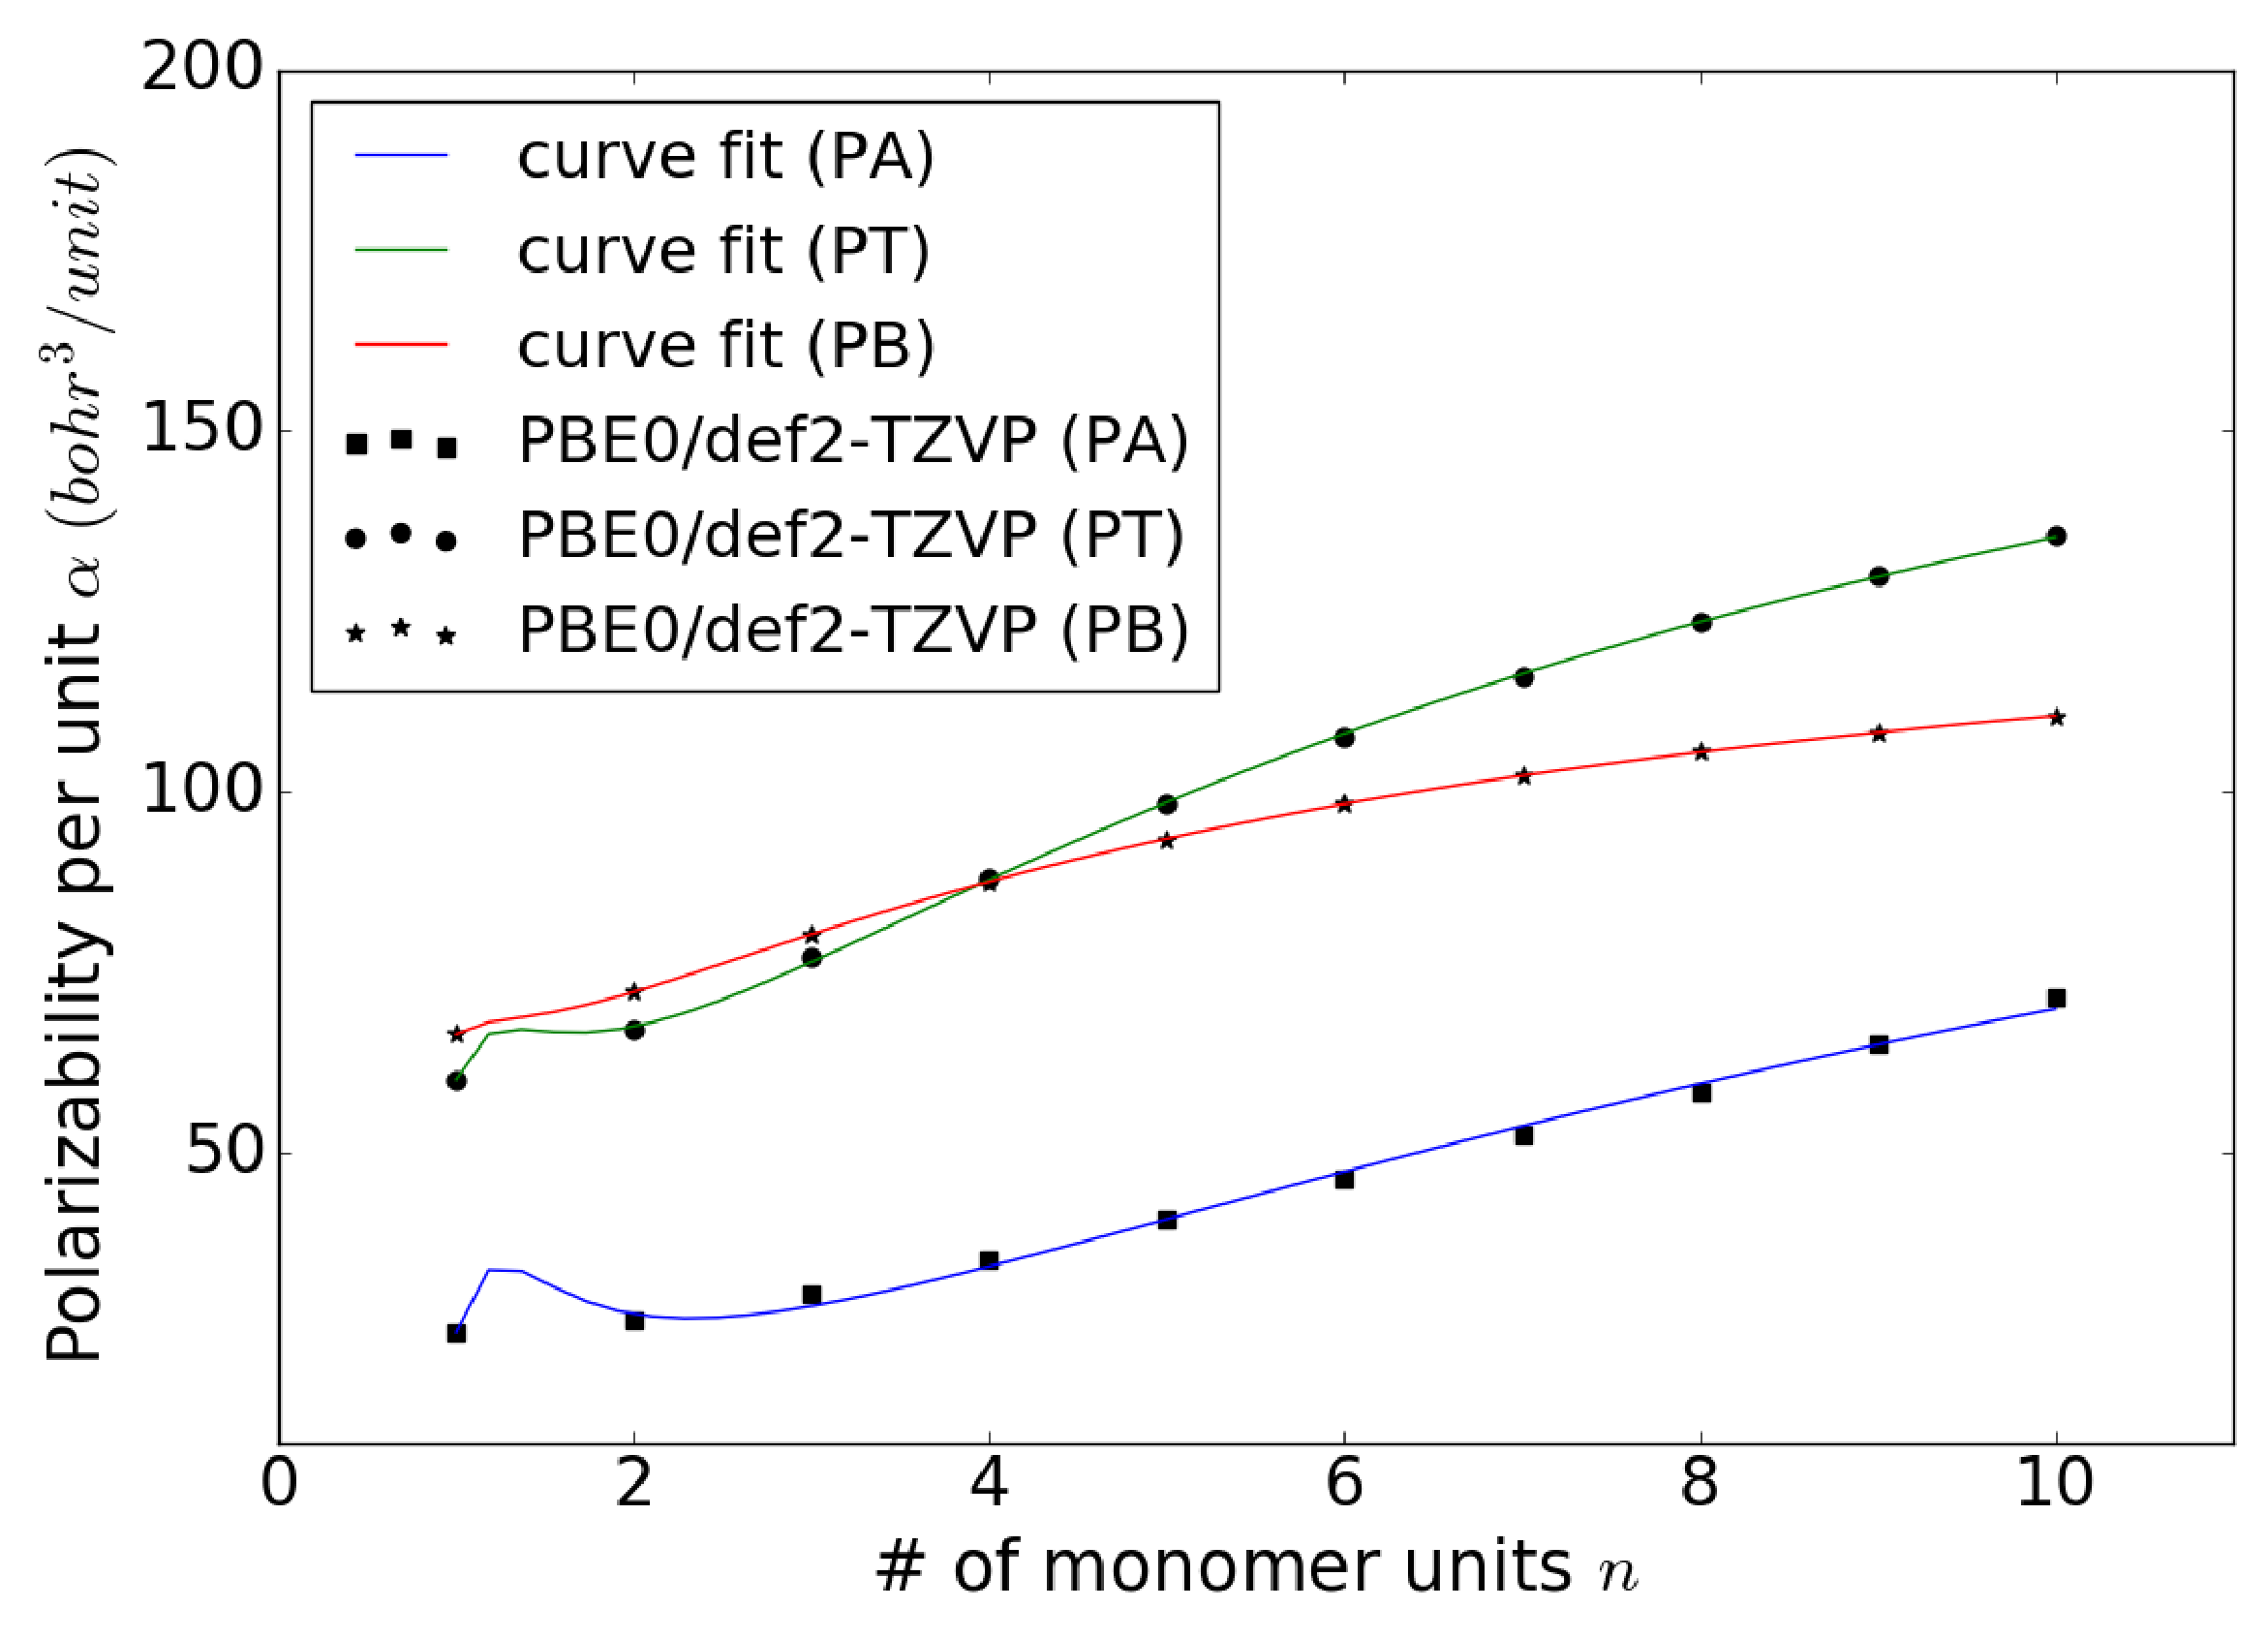
\includegraphics[width=0.744\textwidth]{Chapter-3/Figures/Pol_fit_all_PBE0_TZ.eps}
	\caption{Curve fitting using new polarizability expression for the conjugated polymers polyacetylene (PA), poly(1,4-phenylene) (PB) and polythiophene (PT). Polarizability is calculated using PBE0/TZ.} 
	\label{fig:Pol_fit_all_PBE0_TZ} 
\end{figure}  


%Validation of the extrapolation schemes using longer oligomer chains.
To check the validity of the expression, oligomers up to a chain length of 50 were created. It should be noted that these oligomers were not geometry optimized. The bond lengths and angles were selected based on the optimized geometry of 10 oligomer chain length. We observed that the expression is valid for very long chain lengths (see fig:\ \ref{fig:Pol_fit_all_long_PBE0_DZ}). Using these extrapolation schemes, the polarizability of polymers can be calculated quickly. Further, these schemes are implemented in the high throughput screening framework to accelerate polarizability for large number of polymers. Using the \chemhtps\ framework, the polarizability values of 112 polymers are determined from 12 different methods.

\begin{figure}[htbp] 
	\centering
	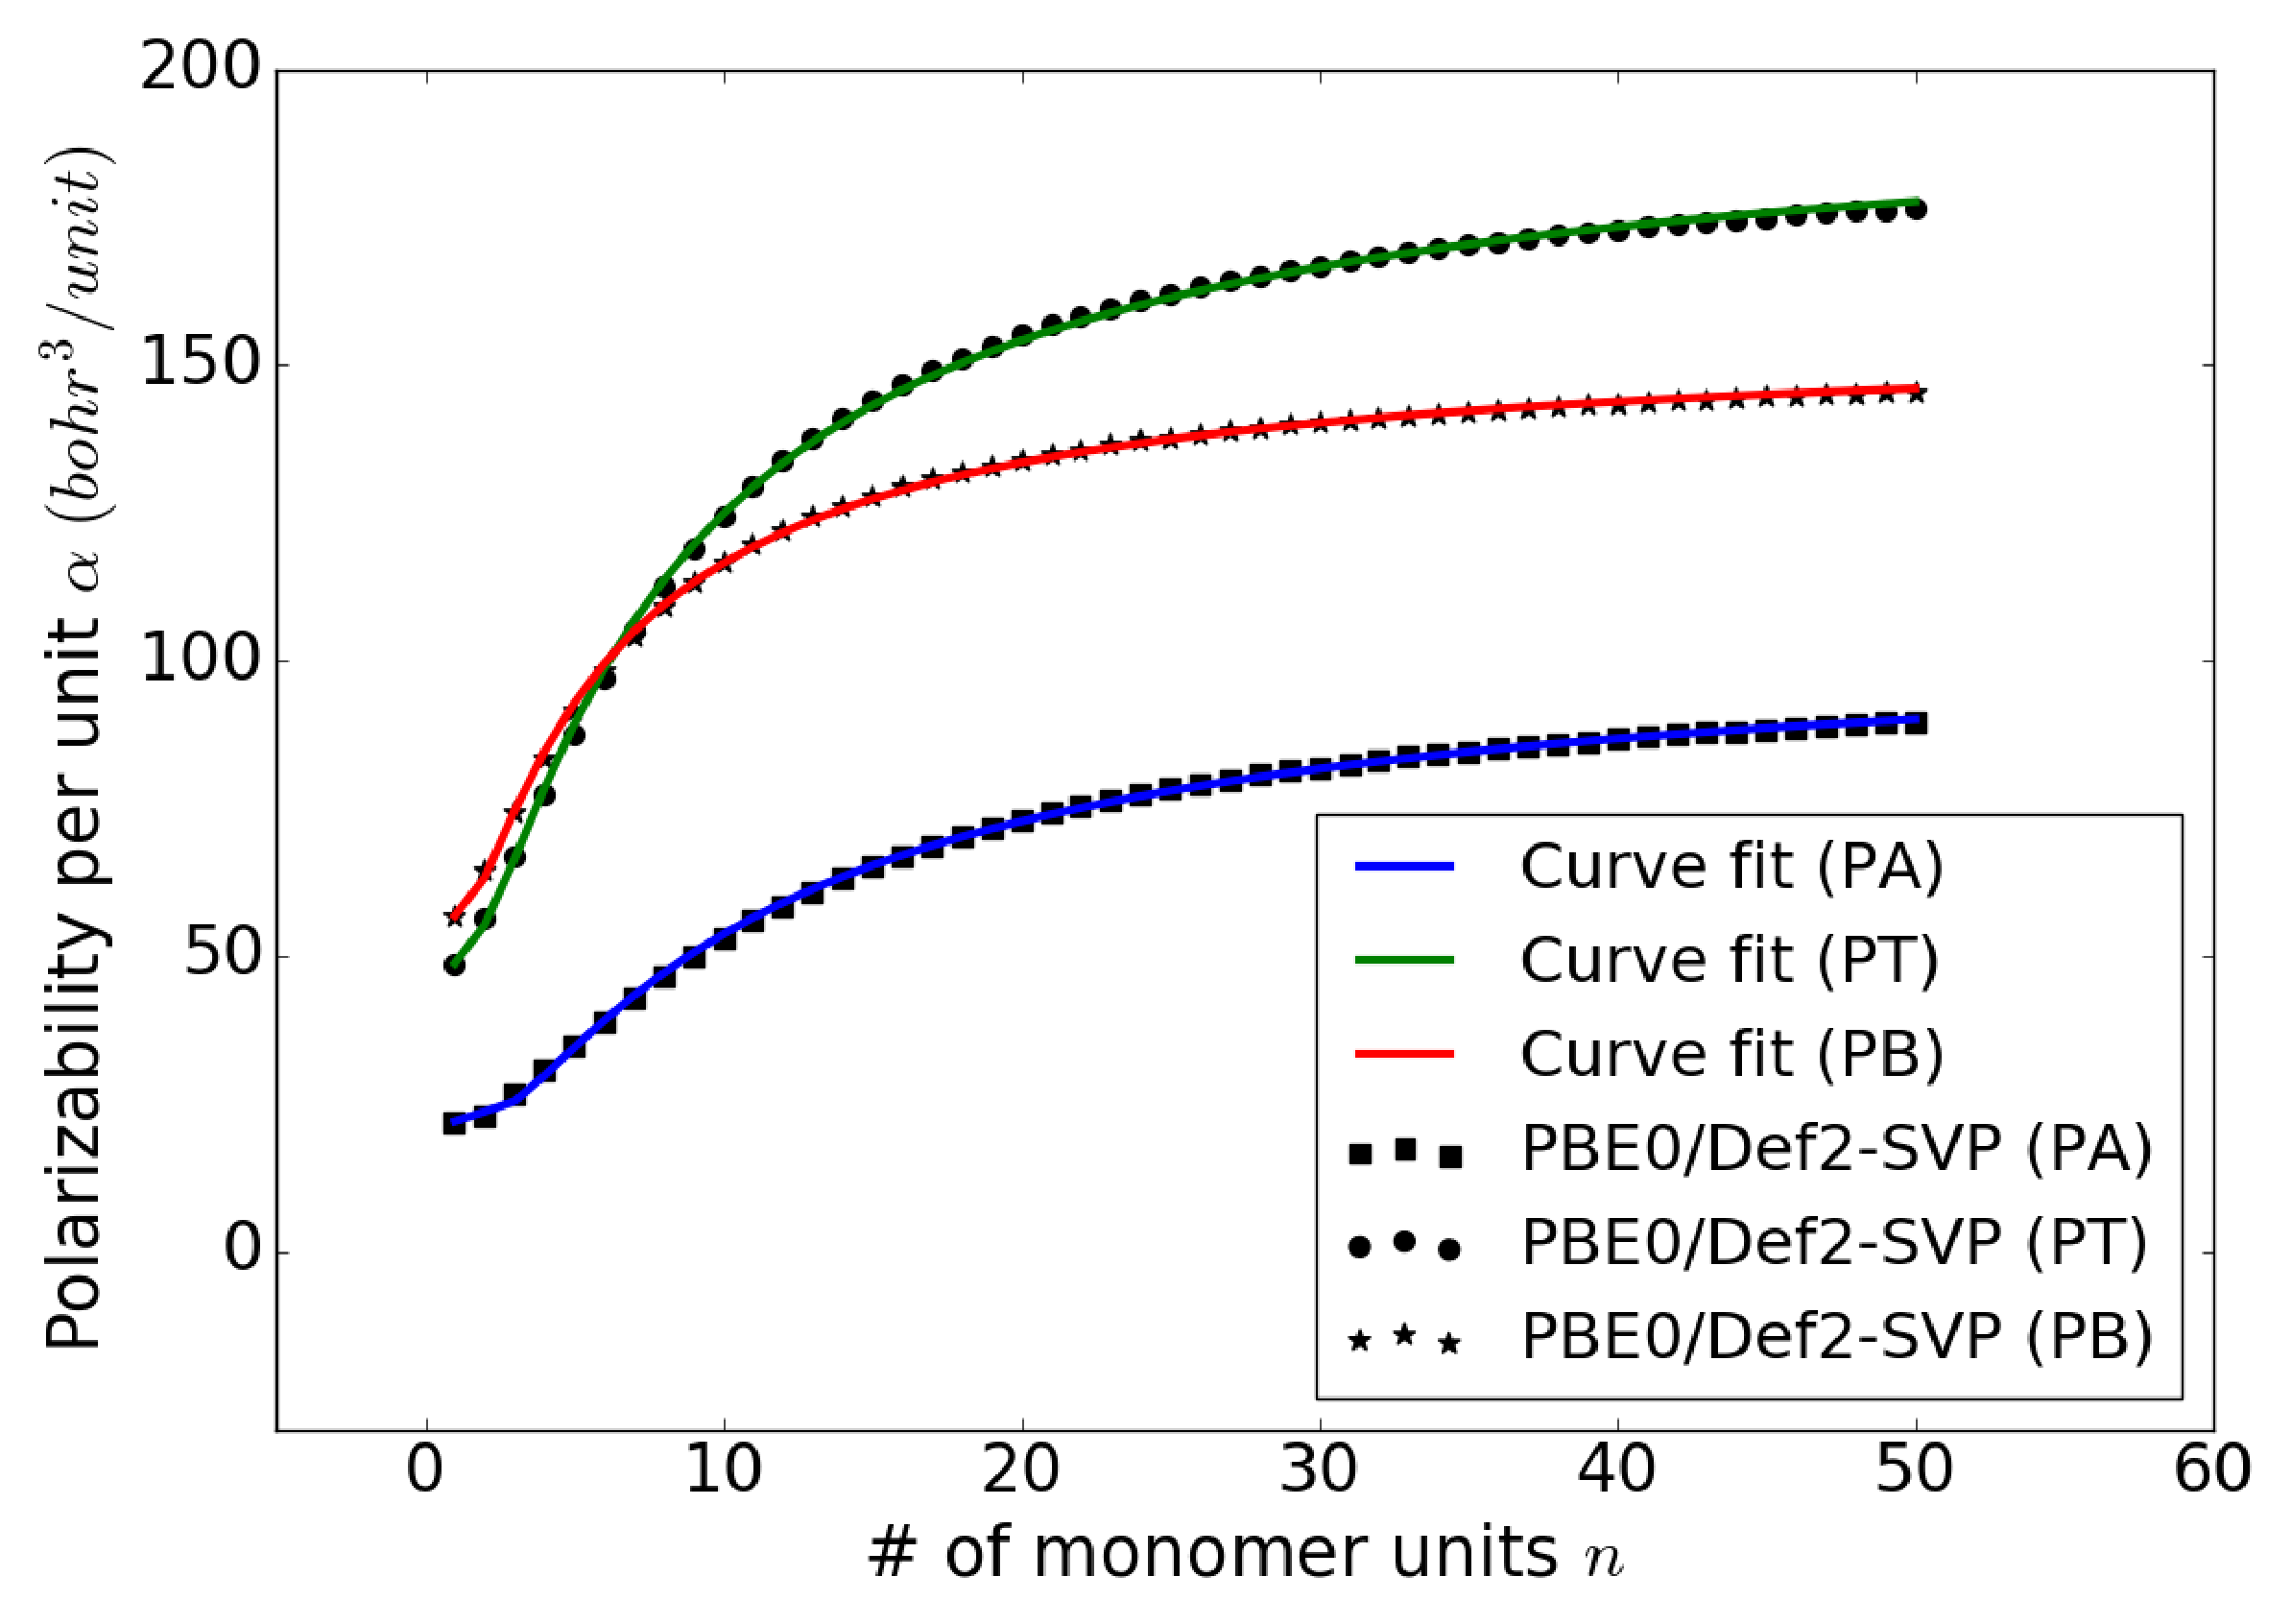
\includegraphics[width=0.744\textwidth]{Chapter-3/Figures/Pol_fit_all_long_PBE0_DZ.eps}
	\caption{Validation of the polarizability expression for long chain lengths of polyacetylene (PA), poly(1,4-phenylene) (PB) and polythiophene (PT). Polarizability calculated using PBE0/DZ} 
	\label{fig:Pol_fit_all_long_PBE0_DZ} 
\end{figure}  

\begin{figure}[htbp] 
	\centering
	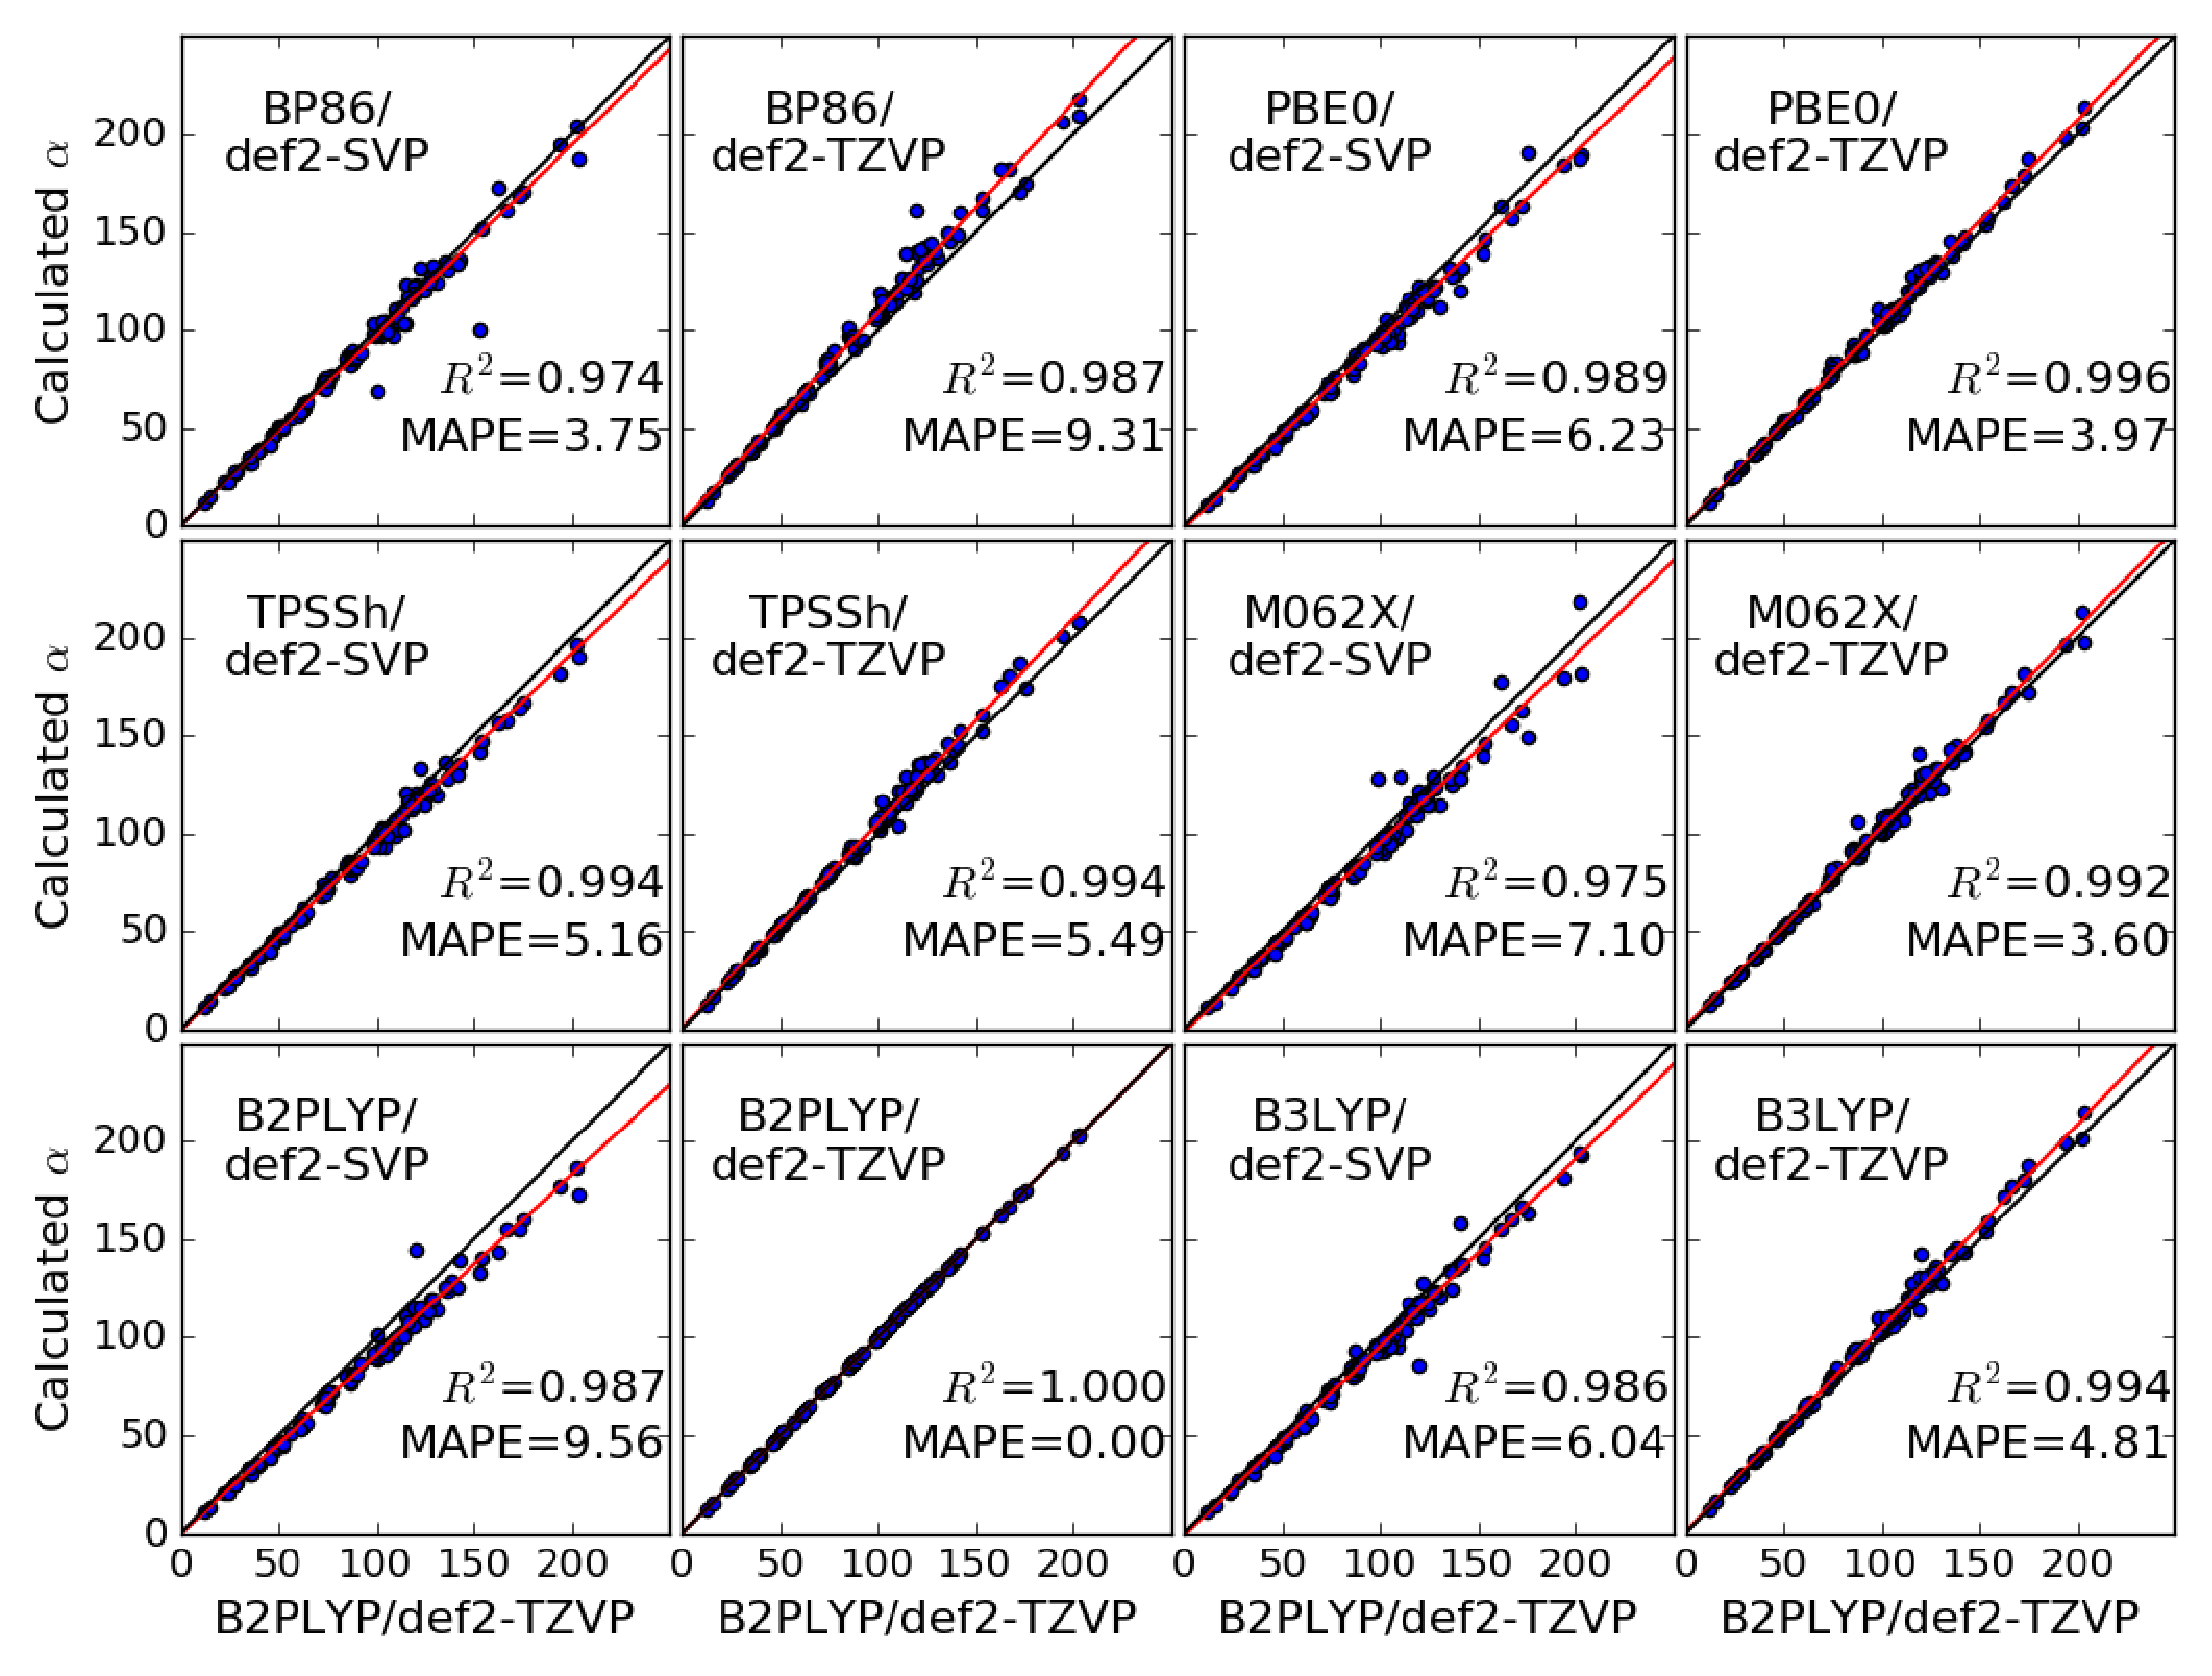
\includegraphics[width=1.00\textwidth]{Chapter-3/Figures/Pol_all_methods.eps}
	\caption{Comparison of polarizability from different methods for 112 polymers with B2PLYP/TZ as a reference.} 
	\label{fig:Pol_all_methods} 
\end{figure}  


%Comparison of polarizability from different methods for all the 112 polymers with B2PLYP/TZ as reference. Finding trends in the results. 

Fig:\ \ref{fig:Pol_all_methods} shows the performance of different model chemistries in comparison to B2PLYP/TZ. Observations from these comparisons are as follows:

\begin{itemize}
\item All the methods have a good correlation ($>$0.975) when compared with B2PLYP/TZ. However, few methods have high MAPE values ($>$5) which is caused due to an offset in the calculation as can be seen from the linear fits of the plots (red lines). For example, the linear fit of B2PLYP/DZ method below the line of symmetry (black line), as most of the values calculated from this method are lower than B2PLYP/def-TZVP. In most of the methods, the offset in the polarizability is larger for higher polarizability values. Therefore, for higher polarizability values, more accurate methods are required.
\item In all TZ calculations, the linear fit is always above the line of symmetry, whereas for all DZ calculations the linear fit is below the line of symmetry. 
\item The correlation for all TZ calculations is better when compared with the DZ calculations.
\item Among the functionals, PBE0 has the best correlation with B2PLYP/TZ and also has a lower MAPE value. Therefore, PBE0 would be a good functional to use for polarizability calculations.
\item The MAPE of B2PLYP/DZ, when compared to B2PLYP/TZ, is 9.56\%.
\end{itemize}

% Benchmarking of RI.  Mathematically discuss how the error in polarizability is translated into RI calculation
The RI ($n$) values are calculated based on the Lorentz-Lorenz equation (see eq: \ref{eqn:3}), which includes the calculation of two different properties, the polarizability ($\alpha$) and number density ($N$). To understand the error propagation from polarizability and number density to RI values, we take a logarithm on both sides of the equation and differentiate to obtain the eq: \ref{eqn:4}.  

\begin{equation} \label{eqn:3}
\frac{(n^{2}-1)}{(n^2+2)}=\frac{4\pi}{3}N\alpha
\end{equation}

\begin{equation} \label{eqn:4}
\frac{dn}{n}=\frac{(1-\frac{1}{n^2} )(1+\frac{2}{n^2})}{6}(\frac{dN}{N}+\frac{d\alpha}{\alpha})
\end{equation}

\begin{equation} \label{eqn:5}
error factor (E)=\frac{(1-\frac{1}{n^2} )(1+\frac{2}{n^2})}{6}
\end{equation}

From eq: \ref{eqn:5}, we observe that the error factor (E) is dependent only on the RI value. For the RI value ranging from 1 to 2, the value of E ranges from 0 to 0.187 respectively (see fig:\ \ref{fig:Error_factor}). Therefore, when the number density error is ignored, the error in RI calculation is less than 20\% of the error in polarizability calculation. For example, if a lower level method, BP86/def-SVP (MAPE 3.75\% compared to B2PLPY/TZ), is used to calculated polarizability instead of B2PLYP/TZ, the additional error in RI calculation would be 0.75\%. This suggests that use of lower level methods for polarizability calculations would not affect RI values significantly.

\begin{figure}[htbp]  
	\centering
	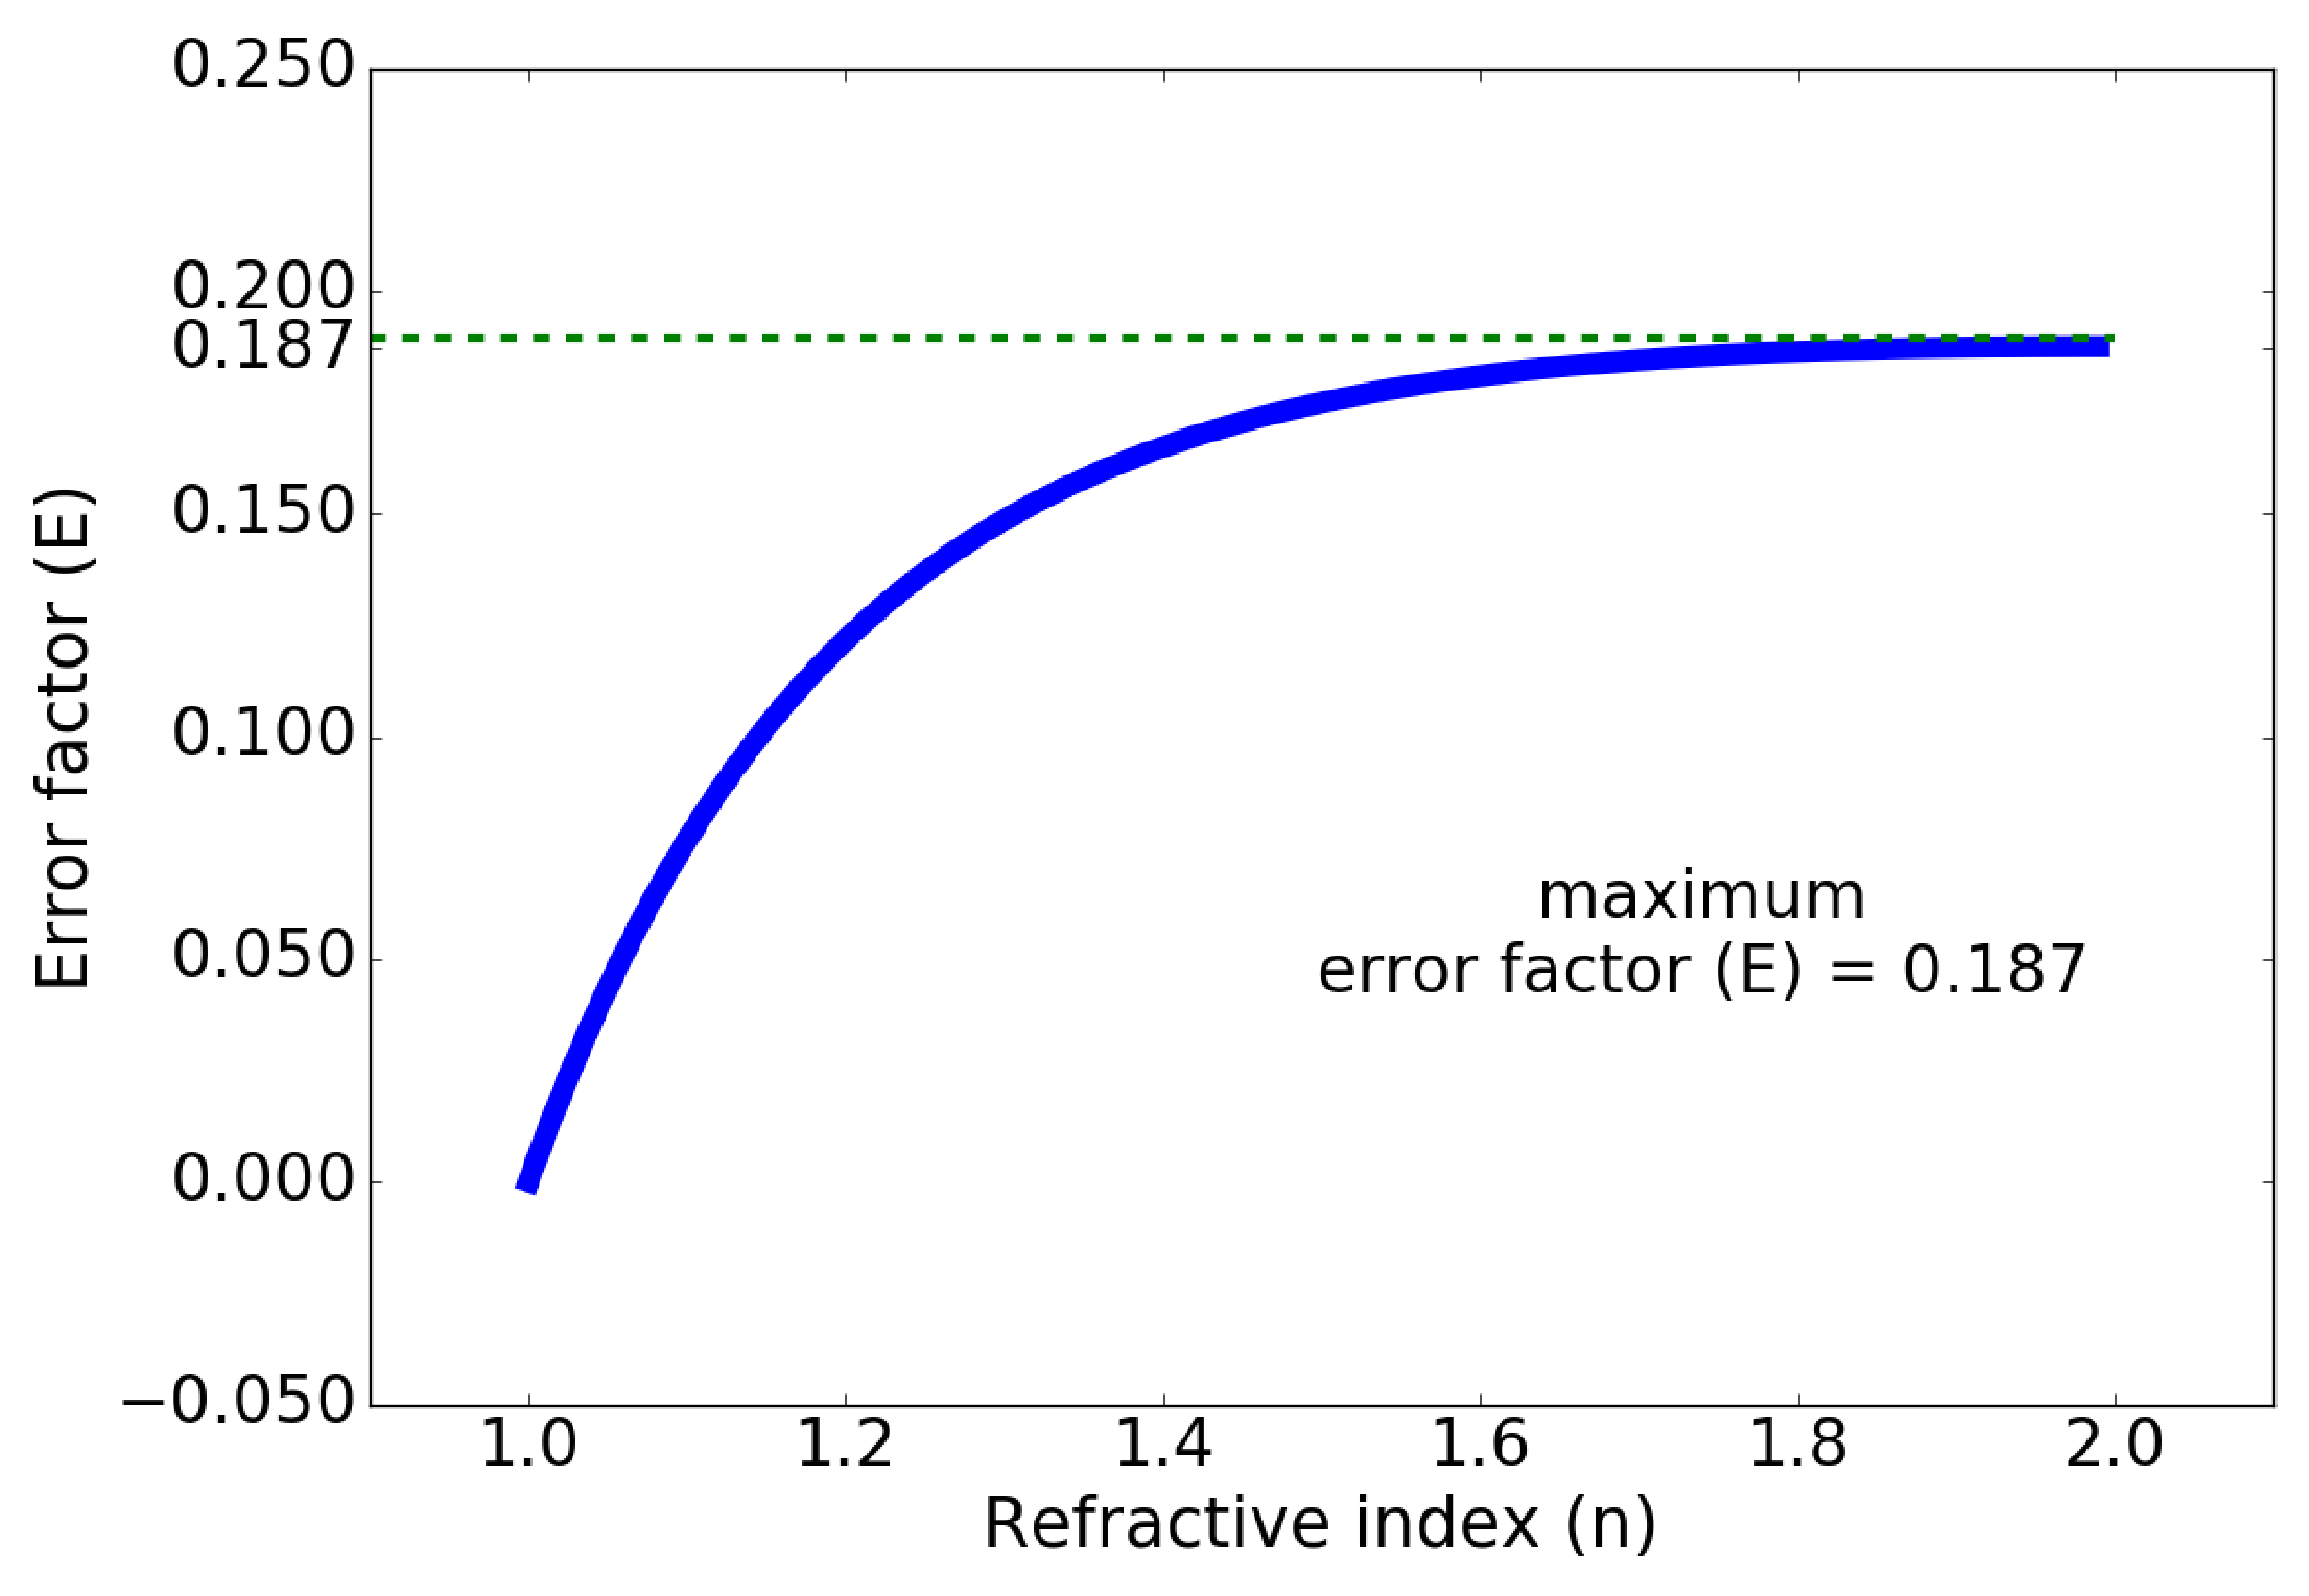
\includegraphics[width=0.744\textwidth]{Chapter-3/Figures/Error_factor.eps}
	\caption{Error factor (E) for RI values ranging from 1 to 2.} 
	\label{fig:Error_factor} 
\end{figure}  

\begin{figure}[htbp] 
	\centering
	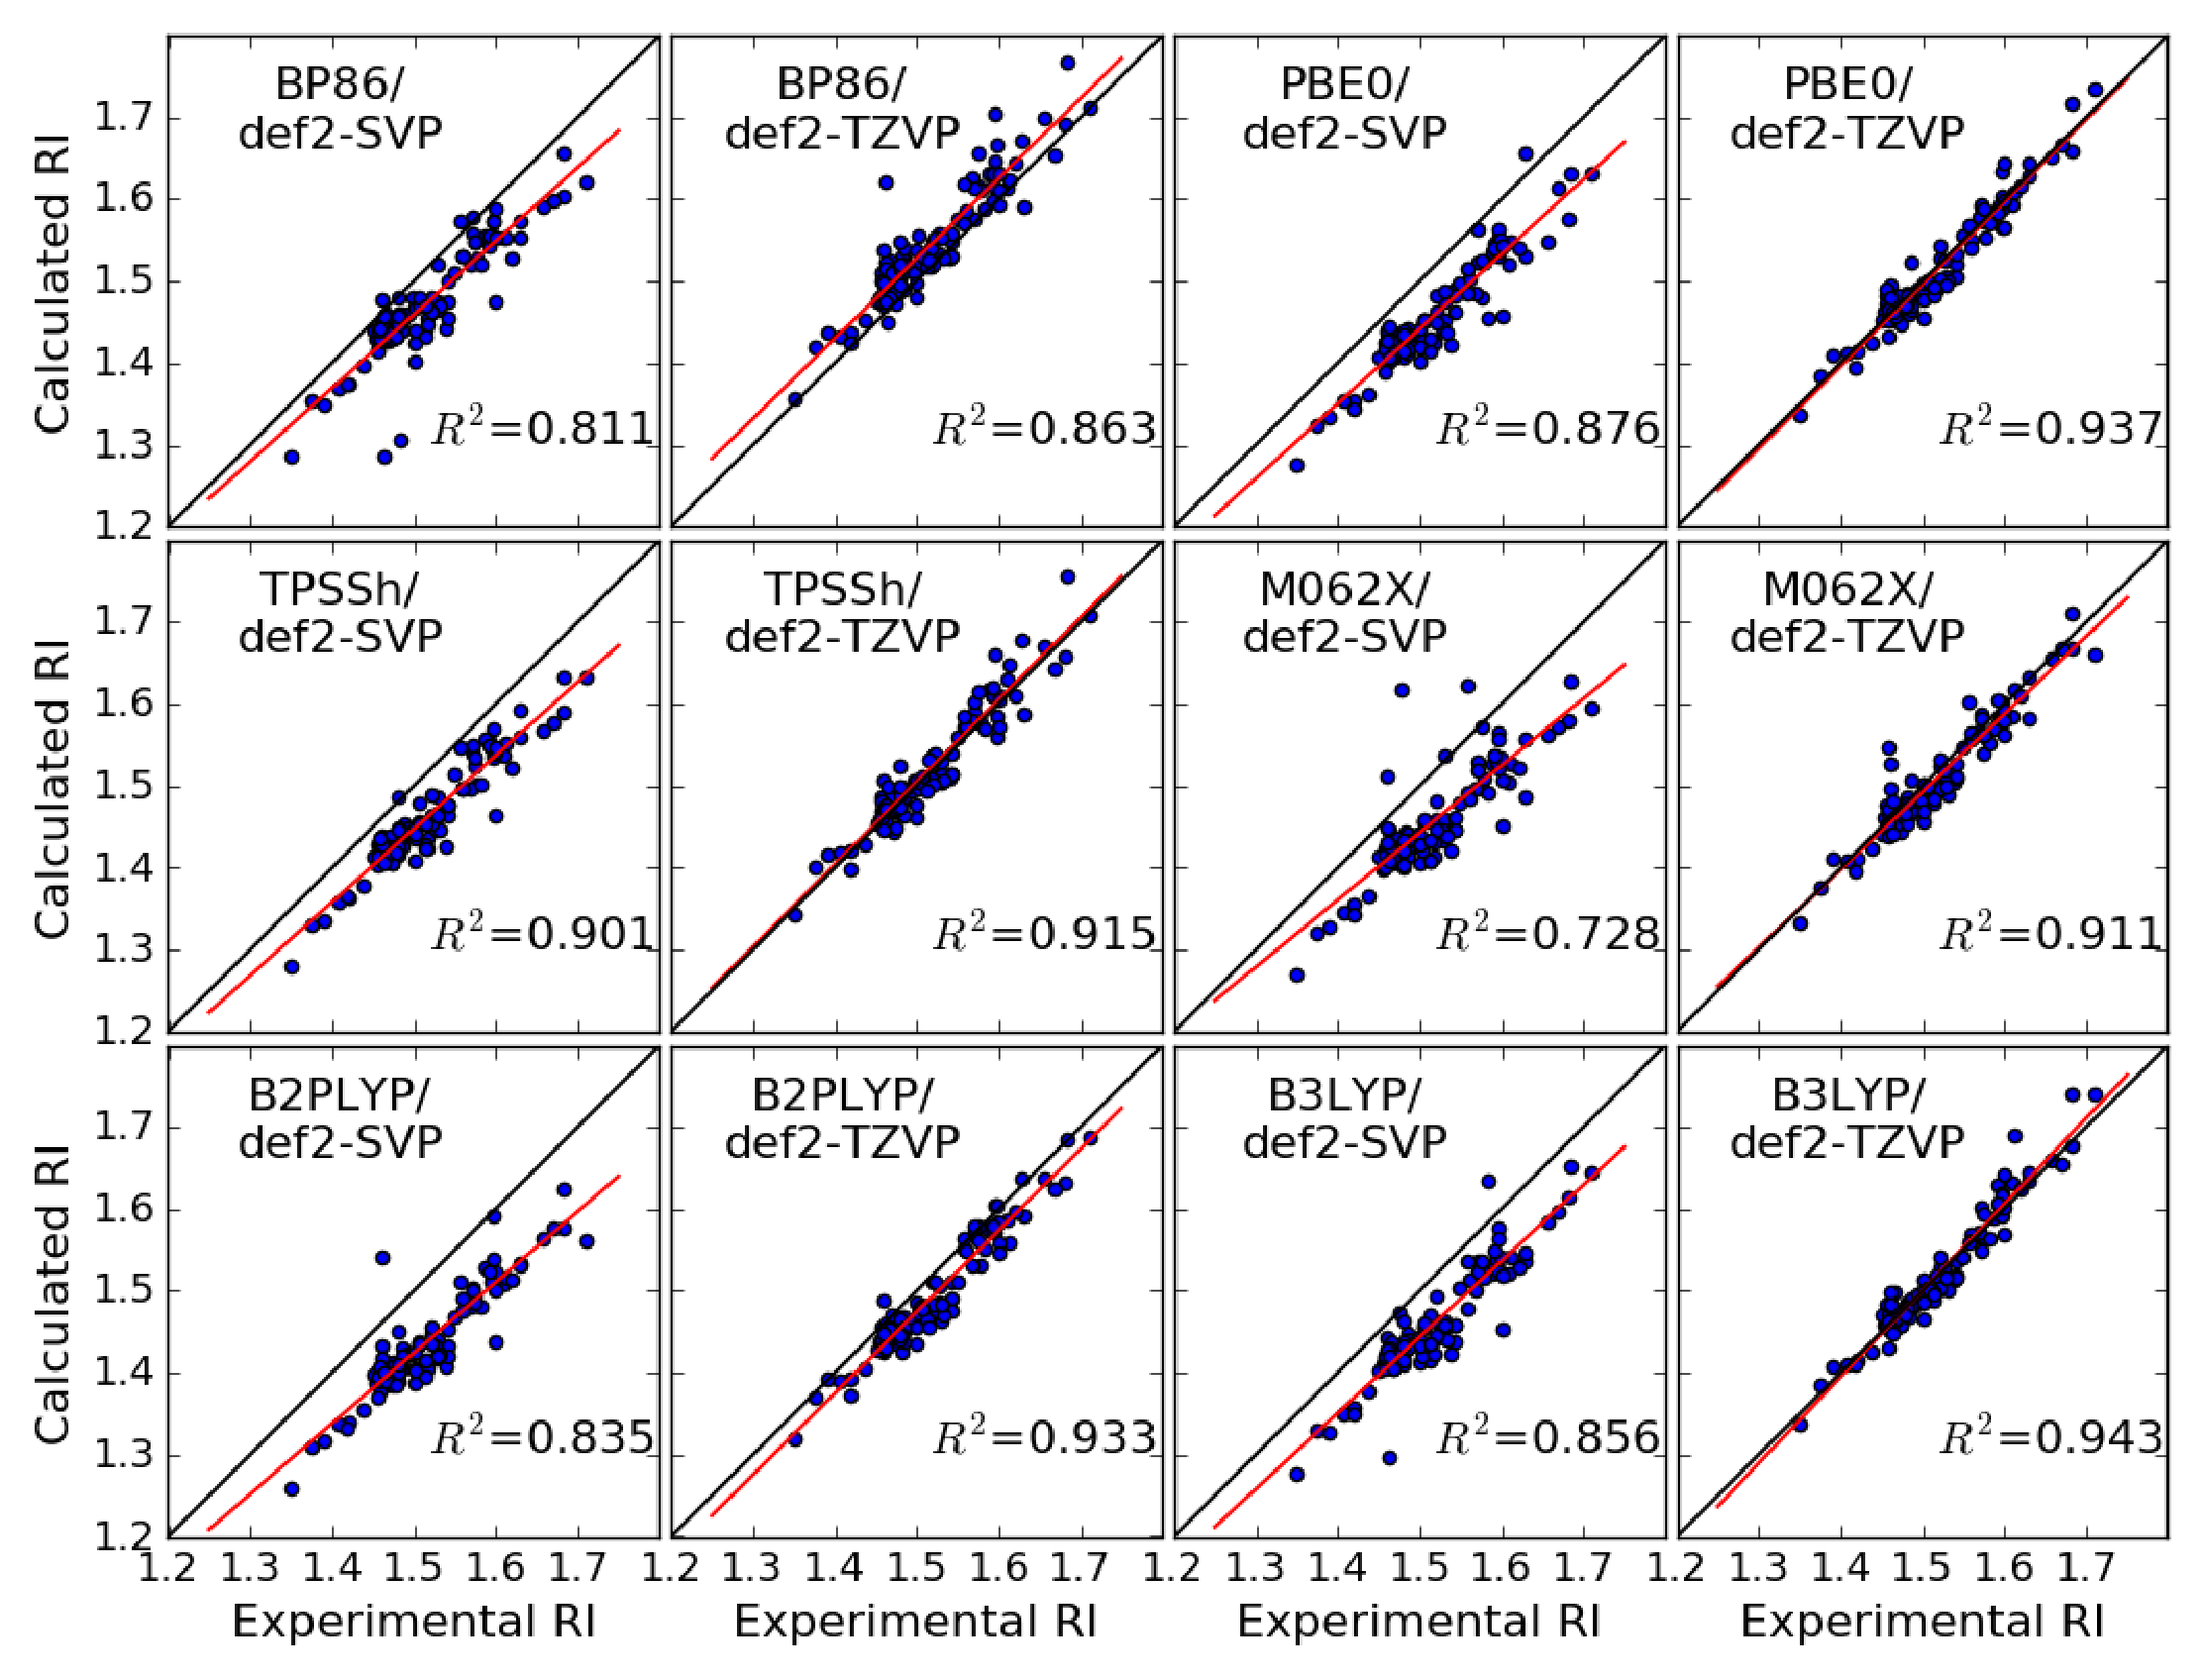
\includegraphics[width=1.00\textwidth]{Chapter-3/Figures/RI_all_methods.eps}
	\caption{Comparison of RI values calculated from different methods for 112 polymers with experimental RI values.} 
	\label{fig:RI_all_methods} 
\end{figure}  



\begin{landscape}
	\begin{table*}[t] 
		\centering
		\caption{Performance of different model chemistries in comparison to experimental values} \label{tab:1}
		\label{my-label}
		\makebox[\textwidth]{\begin{tabular}{ 	p{2.5cm}|p{1.1cm}p{1.1cm}|p{1.1cm}p{1.1cm}|p{1.1cm}p{1.1cm}|p{1.1cm}p{1.1cm}|p{1.1cm}p{1.1cm}|p{1.1cm}p{1.1cm} }
				\hline
				\textbf{Functional}    & \multicolumn{2}{c|}{\textbf{BP86}}                                                                                           & \multicolumn{2}{c|}{\textbf{PBE0}}                                                                                           & \multicolumn{2}{c|}{\textbf{TPSSh}}                                                                                          & \multicolumn{2}{c|}{\textbf{M06-2X}}                                                                                          & \multicolumn{2}{c|}{\textbf{B2PLYP}}                                                                                         & \multicolumn{2}{c}{\textbf{B3LYP}}                                                                                          \\ \hline
				\textbf{Basis set}     & \textbf{\begin{tabular}[c]{@{}c@{}}DZ\end{tabular}} & \textbf{\begin{tabular}[c]{@{}c@{}}TZ\end{tabular}} & \textbf{\begin{tabular}[c]{@{}c@{}}DZ\end{tabular}} & \textbf{\begin{tabular}[c]{@{}c@{}}TZ\end{tabular}} & \textbf{\begin{tabular}[c]{@{}c@{}}DZ\end{tabular}} & \textbf{\begin{tabular}[c]{@{}c@{}}TZ\end{tabular}} & \textbf{\begin{tabular}[c]{@{}c@{}}DZ\end{tabular}} & \textbf{\begin{tabular}[c]{@{}c@{}}TZ\end{tabular}} & \textbf{\begin{tabular}[c]{@{}c@{}}DZ\end{tabular}} & \textbf{\begin{tabular}[c]{@{}c@{}}TZ\end{tabular}} & \textbf{\begin{tabular}[c]{@{}c@{}}DZ\end{tabular}} & \textbf{\begin{tabular}[c]{@{}c@{}}TZ\end{tabular}} \\ 
				\hline
				\textbf{R$^2$} & 0.811           & 0.863           & 0.876           & 0.937           & 0.901            & 0.915           & 0.728            & 0.911           & 0.835            & 0.933            & 0.856            & 0.943           \\
				\textbf{AE}                  & 0.042           & -0.027          & 0.06            & 0.004           & 0.054            & -0.005          & 0.06             & 0.008           & 0.078            & 0.026            & 0.057            & -0.001          \\
				\textbf{MaxE}                & 0.177           & 0.159           & 0.142           & 0.045           & 0.137            & 0.073           & 0.149            & 0.088           & 0.161            & 0.068            & 0.166            & 0.077           \\
				\textbf{SPRE}                & 0.195           & 0.197           & 0.17            & 0.089           & 0.144            & 0.115           & 0.29             & 0.137           & 0.242            & 0.096            & 0.218            & 0.111           \\
				\textbf{MAE}                 & 0.043           & 0.029           & 0.06            & 0.014           & 0.054            & 0.016           & 0.065            & 0.017           & 0.079            & 0.027            & 0.058            & 0.013           \\
				\textbf{MARE}                & 0.028           & 0.019           & 0.04            & 0.009           & 0.036            & 0.011           & 0.042            & 0.011           & 0.052            & 0.018            & 0.038            & 0.008           \\
				\textbf{RMSD}                & 0.052           & 0.038           & 0.064           & 0.018           & 0.058            & 0.021           & 0.07             & 0.022           & 0.082            & 0.031            & 0.063            & 0.018           \\
				\textbf{RMSRE}               & 0.042           & 0.031           & 0.052           & 0.014           & 0.047            & 0.017           & 0.056            & 0.018           & 0.067            & 0.025            & 0.051            & 0.014           \\
				\textbf{Slope}               & 0.9             & 0.98            & 0.91            & 1               & 0.9              & 1               & 0.82             & 0.95            & 0.86             & 0.99             & 0.93             & 10.05            \\
				\textbf{Intercept}           & 0.11            & 0.06            & 0.07            & -0.01           & 0.1              & 0               & 0.21             & 0.07            & 0.13             & -0.02            & 0.05             & -0.08          
			\end{tabular}}
		\end{table*}
	\end{landscape}

%Calculating RI and comparing with experimental results of RI of these polymers.
The RI values for the 112 polymers is calculated using six functionals (BP86, PBE0, TPSSh, M06-2X, B2PLY and B3LYP) and two basis sets (DZ and TZ). The correlation with experimental values and the error analysis of each of these methods is shown in the table \ref{tab:1}. 

Observations:

i. In all the cases, TZ calculations are better than the DZ calculations. 

ii. The functionals B2PLYP, B3LYP and PBE0 have relatively better performance, whereas the M06-2X functional has the worst performance. 

iii. Comparing all the methods, the $R^2$ value for B3LYP/TZ is the highest. This method also has the lowest AE, MAE and MARE. However, the lowest maximum error is observed for PBE0/TZ. 

iv. All the methods showed a maximum error less than 0.2, with a lowest error of 0.045 for PBE0/TZ. Further, the SPR error for this method is 0.089, which suggests that this method is accurate for RI calculation. 

v. If only DZ is considered, then PBE0 and TPSSh functionals have the better performance compared to other functionals. 

vi. The slope and intercept of the linear correlations for the methods TPSSh/TZ, B2PLYP/TZ and PBE0/TZ are 1 and 0 respectively, suggesting that the linear correlation is exact. This can be observed in Fig.\ \ref{fig:RI_all_methods}, where the linear fit (red line) overlaps the line of symmetry (black line).  Thus, the calculated values do not have to be corrected by a factor for these methods. For all the other methods except B3LYP/TZ, the slope is less than 1, which shows that these methods under-predict the RI of polymers with high RI values.

vii. Considering the time of calculations v/s the accuracy of the methods, PBE0/DZ and TPSSh/DZ show the best promise for RI calculation. 

%Discussion on how these benchmarking results will enhance the performance in terms of high-throughput screening of potential candidates.
Now that we have developed a robust protocol for RI prediction of polymers, our next step is to cast these into our automated high-throughput framework, and employ in on an extensive candidate screening library. We plan to apply this framework to discover high RI polyimides and polyenes. The candidate library of these polymers will be created from promising building blocks using our combinatorial library generator. We will also pursue the development of a smart, responsive, and thus more efficient scheme in the course of the project, which will avoid the problems of exponential growth. The different screening phases will successively reduce the pool of viable candidates. The resulting data will be analyzed, mined, and modeled using machine learning and informatics techniques to extract structure-property relationships.



% ...

\section{Conclusions}
\label{sec:conclusions3}

We have successfully created 270,000 novel PI candidates, and evaluated the RI values of these candidates by casting into \chemhtps. From the screening studies, we found PI candidates that possess RI values greater than 1.8. 
Z-score analysis showed that prevalence of certain building blocks ( \eg building blocks 25 and 28) in a top candidates. In addition to identifying individual building blocks that are promising for high RI polymers, promising building block pairs are also identified.  Z-score value. We observed that the combination of building block 28 with blocks 2 and 3 to be highly promising in the design of HRIPs. Thus, we successfully identified favorable building blocks and synergy between building blocks combinations for developing high RI PIs. We demonstrated that our cyberinfrastructure is a powerful tool and has shown to be highly promising for identifying polyimides with exceptional RI values.
\chapter{Molecular Library Generator and Virtual High-Throughput Screening Framework}
	
%\chapter{Rational Design Framework for Accelerating the Discovery of Materials}

The discovery of new compounds, materials, and chemical reactions with exceptional properties is the key to progress in chemistry. This process can be dramatically accelerated by means of the virtual high-throughput screening of large-scale candidate libraries. This approach has been extensively used for many years in the drug discovery community and has more recently been applied to the search for energy materials. The key challenge is that chemical space is practically infinite, and any approach to survey it or enumerate certain of its domains has to address the problem of combinatorial complexity.

Therefore, we have developed a general-purpose suite, \chemlg , a generator for compound and material candidate libraries. In this chapter, we primarily discuss the algorithms implemented in \chemlg, and give examples of its successful application in various domains. We also briefly discuss the other three software packages in our group's software ecosystem, \chemhtps, \chembddb, and \chemml.

I am the primary developer of \chemlg\ code. The code \chemhtps\ was co-developed with William Evangelista. The developers of \chembddb\ are Aditya Sonpal and Shirish Sivaraj, whereas the primary developer of \chemml\ is Mojtaba Haghighatlari. 

\section{Introduction}

A prerequisite for the high-throughput exploration of chemical space is access to suitable, large-scale screening libraries. The key for a successful library generation approach is to balance the ambition for a systematic and exhaustive enumeration of the combinatorial search space, with the need for an efficient and responsive scheme. The generation of combinatorially exhaustive libraries is relatively straightforward, but it rapidly becomes impractical for screening purposes due to its exponential growth. For instance, the largest small-molecule library, GDB-17, contains 166.4 billion molecules, which were generated using only up to 17 atoms (C, N, O, S, and halogens) \cite{Reymond2012}. Most currently available codes are thus limited to generating small, drug-like molecules. 

\chemlg\ extends and generalizes the molecular library generation to identify lead candidates in various applications such as functional polymers, optoelectronics, and catalysis. It offers a multitude of options to customize and restrict the scope of the enumerated chemical space and thus tailor it for the demands of specific applications. To streamline the non-combinatorial exploration of chemical space, we incorporate genetic algorithms into the framework. Genetic algorithms have shown to be efficient in optimizing chemical structures and generating useful compounds for different target applications. In addition to implementing smarter algorithms, we also focus on the ease of use, workflow, and code integration to make this technology more accessible to the community. 


\section{Methodology}

There are two different approaches for enumeration of compound space: product-based approach and reaction-based approach. The former one is based on the application of Markush structures, which expands the library by attaching the functional groups to various sites on the scaffold whereas the latter approach is based on chemical transformation [4]. Combinatorial libraries can be obtained by using three different algorithms: the first is the ‘grow’ algorithm where the growth in the molecule starts from a seed point, second is the ‘fragment-link’ algorithm and the third algorithm is the sampling approach where the growth of the molecules is based on random selection [5]. In our generator, we use the ‘fragment-link’ method which follows a reaction transform approach. The reaction can be obtained by two methods: first method is the reshuffling of the SMILES strings and the second method follows an actual reaction scheme. Both of these methods are discussed in the following subsections. 

\subsection{SMILES Rearrangement}

SMILES, which stands for simplified molecular-input line-entry system, is a string notation for describing the structure of chemical species \cite{Anderson1987}. It is a widely used notation as it is human readable and can be imported by most molecule editors for molecular visualization. In the SMILES rearrangement method, the SMILES of the linking molecules is written such that the linking atoms are positioned at the extreme end of the string. The linkage can then be obtained by directly combining the SMILES strings. A schematic representation of this method is shown in the Fig.\ \ref{fig:validation}. In this method, it is not necessary to specify reaction sites or have to use any reaction algorithm. This way of linkage can generate all possible combinatorial structures. 

\begin{figure}[htbp] 
	\centering
	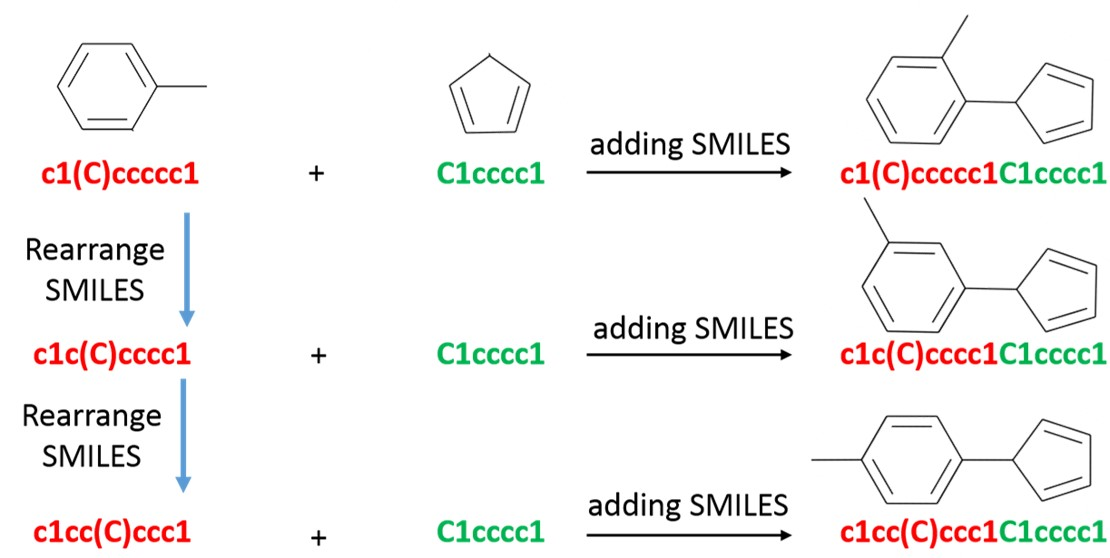
\includegraphics[width=0.9\textwidth]{Chapter-4/Figures/SMILES_link.jpg}
	\caption{Fragment linkage based on SMILES rearrangement.} 
	\label{fig:SMILES_link} 
\end{figure}  

We developed a code to represent the SMILES of a molecule with all possible string notations in which the chemical handles are positioned on the extremes. This method is extremely powerful as it can produce a large molecular library spontaneously. Further, this method is more suited for the generation of polymer libraries. We apply this method to generate a library of polyimides for the exploration of high-refractive-index polymers discussed in Chapter 5. However, there are a few limitations to this approach. For example, a large number of duplicates will be generated in the process and the removal of duplicates will be computationally expensive. Additionally, narrowing the chemical space will be difficult as applying constraints on string notations is challenging. Further, the generation of fused molecules is not possible using this approach.

\subsection{Fragment Link and Fusion}

Fragment link or fusion of fragments is performed by casting into a reactor. The reactor in \chemlg\ takes the fragments as arguments along with combination type and generates a linked or fused molecule. A schematic representation for the link and fusion of molecules is shown in the Fig.\ \ref{fig:link+fusion}. In this scheme, the reaction sites on the fragments are denoted as X. In case of linking, once the reaction occurs, there is a bond formed between the fragments and X is removed. While, in fusion, the molecules lose two carbons and a hydrogen along with X.

\begin{figure}[htbp] 
	\centering
	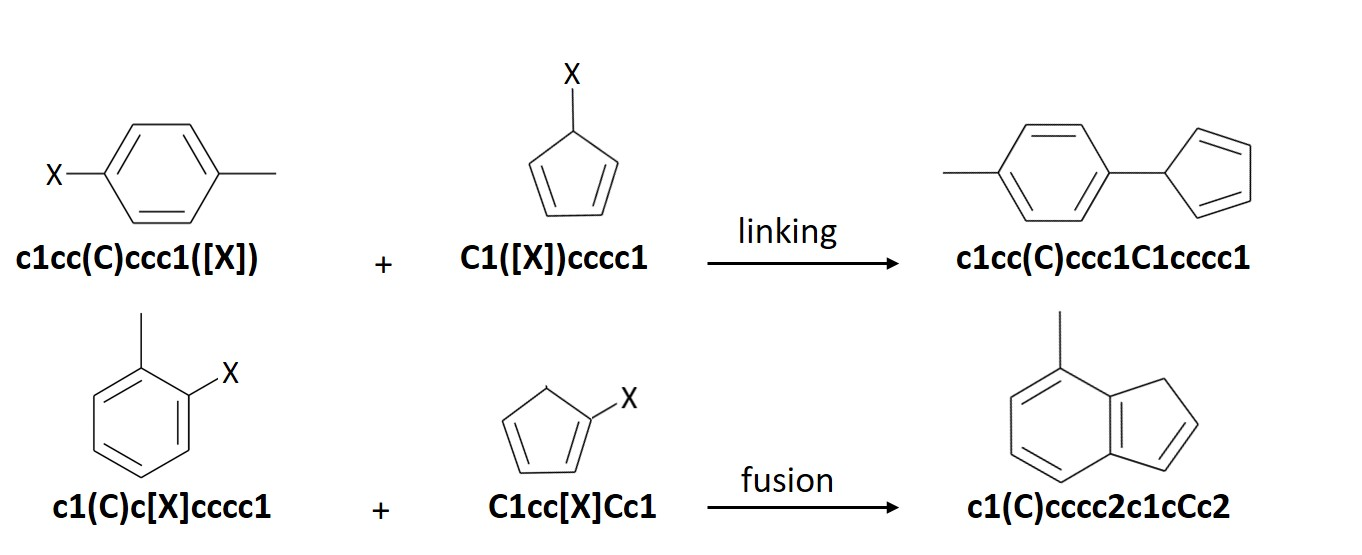
\includegraphics[width=0.9\textwidth]{Chapter-4/Figures/link+fusion.jpg}
	\caption{Schematic for the link and fusion of molecules in \chemlg.} 
	\label{fig:link+fusion} 
\end{figure}  

\section{Generation Constraints}

We find that instead of exploring a limited chemical domain exhaustively, it is often more useful to bias the search in directions where candidates are most promising and synthetically viable. In our development of \chemlg\ , we have thus augmented the combinatorial schemes by a number of `smart' modules that make use of additional input. To address the concern that virtual candidates may not be accessible or desirable (\eg  from a synthetic perspective), we have introduced a constrained-growth scheme that continually prunes the generation process. In this scheme, molecules are rejected at every generation to constrain the growth as shown in the Fig.\ \ref{fig:constrained}. It accepts user-defined constraints, \eg  to exclude certain structural patterns or substructures, fingerprint matching, building block combinations, or sequences; to limit size or chemical makeup; or to enforce symmetries or other rules (\eg  Lipinski's rule).
%\begin{enumerate}
%	\item Include building blocks
%	\item Min and max no. of bonds 
%	\item Min and max no. of atoms 
%	\item Min and max mol. weight 
%	\item Min and max no. of rings 
%	\item Min and max no. of aromatic rings
%	\item Min and max no. of non-aromatic rings
%	\item Min and max no. of single bonds 
%	\item Min and max no. of double bonds
%	\item Min and max no. of triple bonds
%	\item Max no. of specific atoms
%	\item Lipinski's rule
%	\item Fingerprint matching
%	\item Substructure
%	\item Substructure exclusion
%\end{enumerate}

\begin{figure}[htbp] 
	\centering
	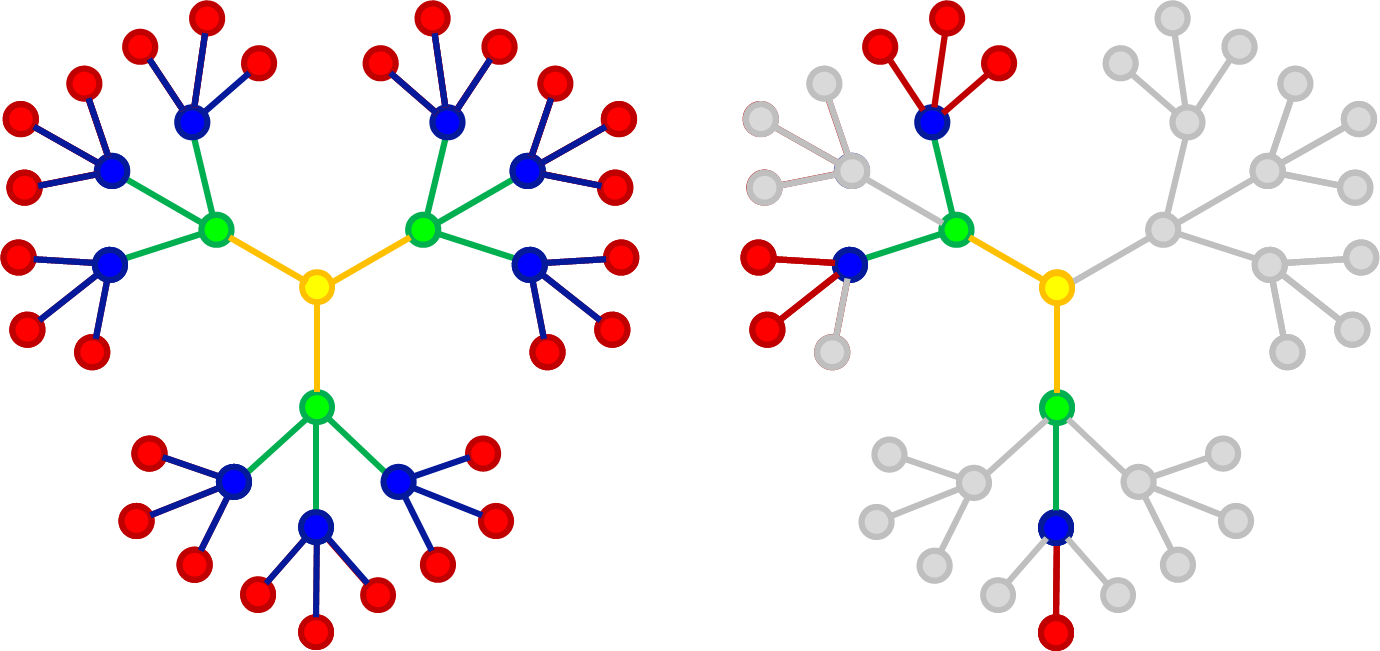
\includegraphics[width=0.9\textwidth]{Chapter-4/Figures/constrained.png}
	\caption{Schematic for constrained growth of molecular library. The left scheme shows an exhaustive enumeration, whereas the right scheme represents a targeted enumeration.} 
	\label{fig:constrained} 
\end{figure}  

\section{Smart Algorithm}
Even applying above mentioned generation constraints might lead to a large number of unwanted molecules in the library. We need to only target the molecules that are of interest and discard the rest. Application of smart algorithms can narrow down the chemical space to a more specified regions. A schematic for the pruning of molecular libraries is shown in Fig.\ \ref{fig:smart_algo}. \chemlg's genetic algorithm module allows us to optimize candidate pools and the chemical structures they contain for specific target applications. 

\begin{figure}[htbp] 
	\centering
	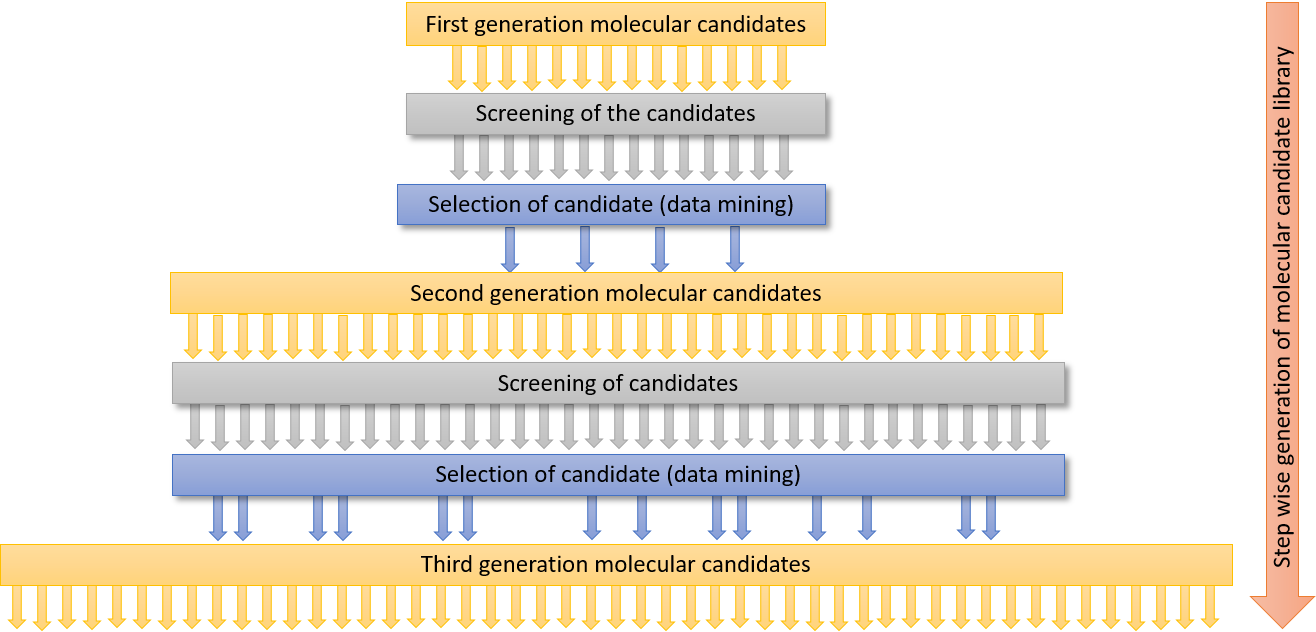
\includegraphics[width=0.9\textwidth]{Chapter-4/Figures/smart_algo.png}
	\caption{Pruning of molecular library at every generation by use of smart algorithms.} 
	\label{fig:smart_algo} 
\end{figure}  

We employ an on-the-fly prescreening through rapid candidate assessment \via\ DFT, MD, or data-derived prediction models. These models also serve as fitness functions in \chemlg 's genetic algorithm module, which allows us to optimize candidate pools and the chemical structures they contain for specific target applications. In genetic algorithm approach, at every generation of molecular library, best candidates are retained and certain operations are performed to generate new promising candidates. These operations include crossover and mutation (see Fig.\ \ref{fig:GA}). In the crossover operation, the structures from top candidates are split and exchanged with each other. Whereas in mutation, randomly selected substructure is replaced with other building blocks from the initial list. Following this scheme for several generations will result in a library that is tailored for a targeted application. As an example, this scheme is applied to create a library of molecules with similar structure to a targeted molecule with fingerprint matching as fitness function (see Fig.\ \ref{fig:GA_example}). We observe that at every generation we obtain molecules that match better to the target molecule. 


\begin{figure}[htbp] 
	\centering
	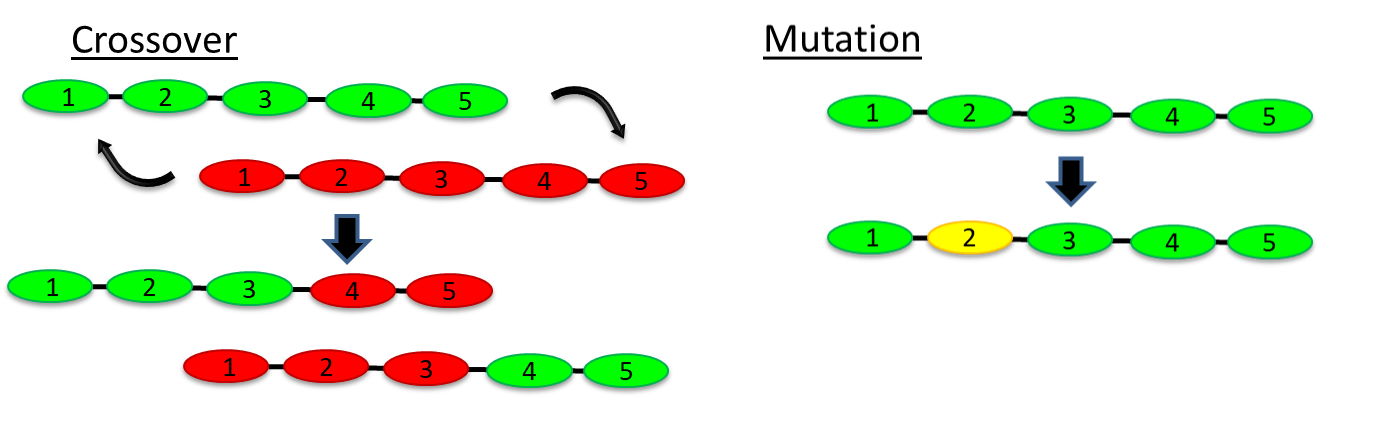
\includegraphics[width=0.9\textwidth]{Chapter-4/Figures/GA.png}
	\caption{Genetic algorithm operations: crossover and mutation.} 
	\label{fig:GA} 
\end{figure}  


\begin{figure}[htbp] 
	\centering
	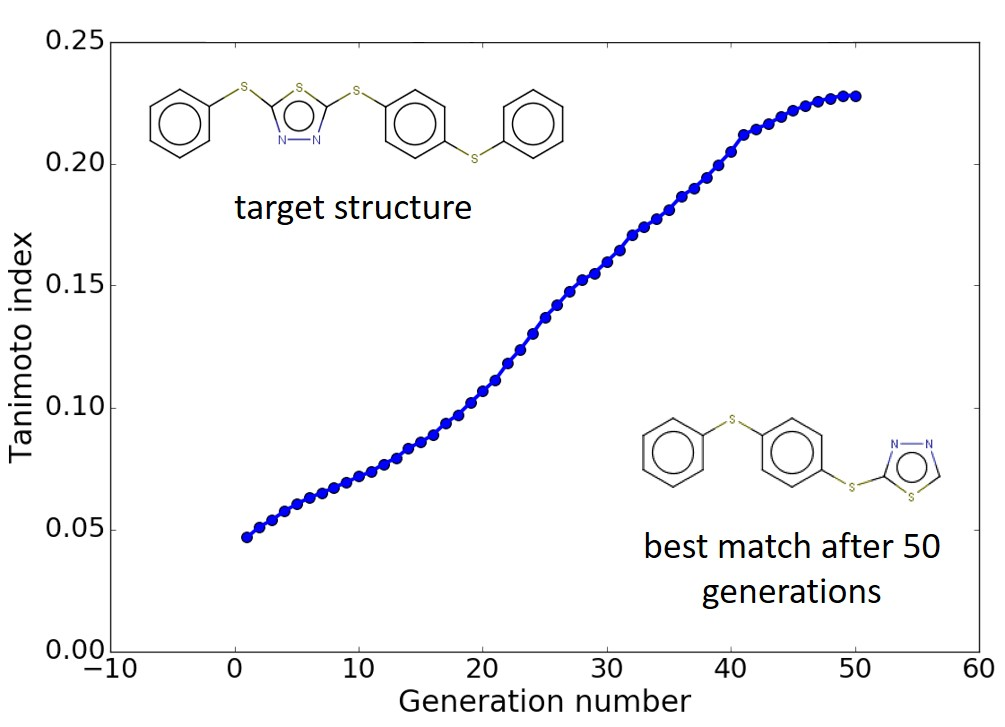
\includegraphics[width=0.75\textwidth]{Chapter-4/Figures/GA_example.jpg}
	\caption{Implementation of genetic algorithm to find similar structures.} 
	\label{fig:GA_example} 
\end{figure}  


\chemlg 's `smart' modules can thus facilitate self-regulating growth of the candidate libraries and ultimately a self-optimizing traversal of chemical space. It offers options for the various approaches mentioned above to provide the most suitable solution for different problem settings. We have successfully employed \chemlg\ to produce screening libraries for a number of application projects.


\section{Parallel Implementation of \chemlg}

An important feature of \chemlg\ is that the code is massively parallel. The parallelization is obtained using MPI4Py library and it is implemented at various levels to accelerate the library generation process (see Fig.\ \ref{fig:ChemLG_parallel}). This allows us to create a library of millions of molecules in just a few seconds. The bottleneck step is the removal of duplicates at every level. There are several algorithms for efficient removal of duplicates, but they are designed to run in a serial fashion. Parallelizing these algorithms is not efficient as there is significant communication overhead in the process. For efficiently scraping duplicated in molecular library, we exploit the fact that no two molecules with different molecular weights are same. We group the molecules based on their molecular weights by keeping tags and scatter the groups to different processors for duplicates removal. This process is efficient as it involves no communication between the processors. The speedup and parallel efficiency of the code for the generation of a million candidates is shown in Fig.\ \ref{fig:ChemLG_performance}. The performance of \chemlg\ scales very well with increasing number of processors. Due to a high-level of parallelization, \chemlg\ performs well on a high performance computing (HPC) platform. This is helpful as it integrates well with \chemhtps\ infrastructure, where the molecular library can be generated and readily applied for HTPS.

\begin{figure}[htbp]
	\centering
	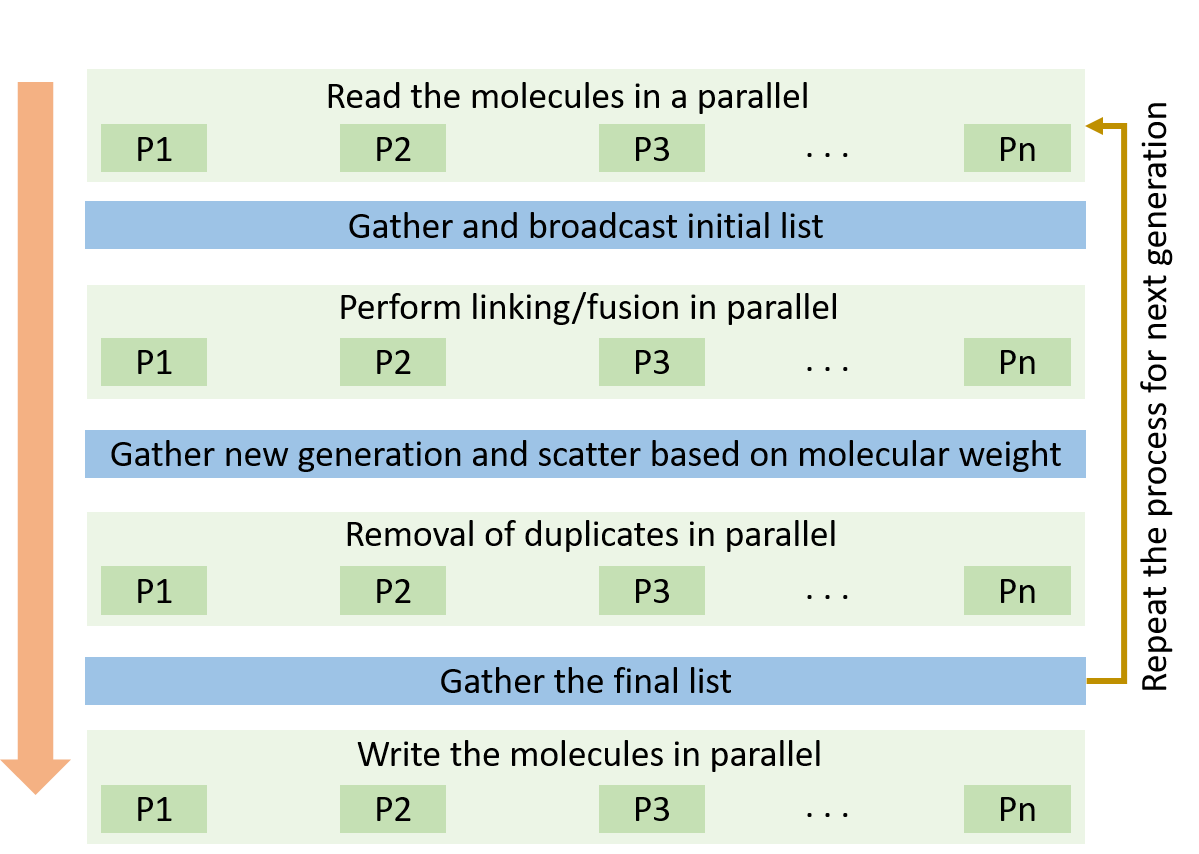
\includegraphics[width=0.75\textwidth]{Chapter-4/Figures/ChemLG_parallel.png}
	\caption{Levels of parallelization in \chemlg\  package.} 
	\label{fig:ChemLG_parallel} 
\end{figure}  

\begin{figure}[htbp] 
	\centering
	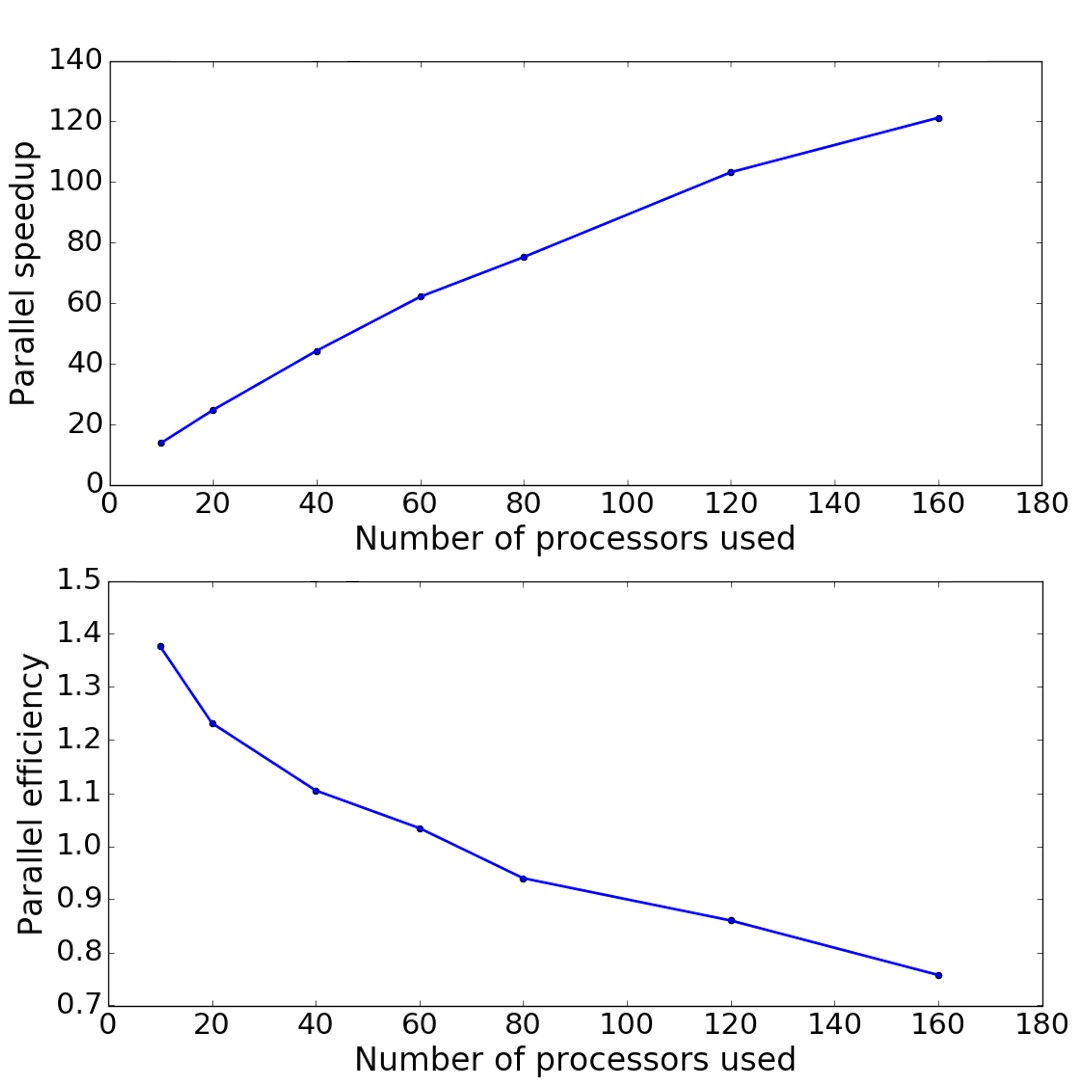
\includegraphics[width=0.7\textwidth]{Chapter-4/Figures/ChemLG_performance.jpg}
	\caption{Parallel speedup and efficiency observed in \chemlg\ package.} 
	\label{fig:ChemLG_performance} 
\end{figure}  

\section{Example Applications of \chemlg}
\label{subsec:chemlg_app}

\chemlg\ has been successfully applied in various applications. In the current dissertation, it is applied to make a library of polyimides and small organic molecules for the exploration of chemical systems with high RI values. Further details of these two libraries are discussed chapter 5 and chapter 6, respectively.

The generator was also used for creating a library of polyesters in a quest to design polymers with superior degradation behavior. We found that the activation energy for the degradation of polyesters is dependent on the functional groups that are attached to the $\beta$-carbon of the ester bond. This results motivated us to generate a library functional groups that can ba attached to $\beta$-carbon. This project is being led by Vigneshwar Kumaran Sudalayandi Rajeswari. 
  
In another project, internship work at ExxonMobil Chemical Company, \chemlg\ was used to create a library of novel polyolefins \cite{Afzal2018d}. The library was built by linking saturated carbon atoms in a combinatorial fashion. We used methane, ethane, and butane as the building blocks while considering all the hydrogens as connection sites. Using these rules, the library was built until three generations, which resulted in 275 monomer structures. These monomers were used to build corresponding oligomers and subsequently screened them in a virtual high-throughput fashion to evaluate their coil dimensions.

\chemlg\ has also been instrumental in formulating chemical libraries for compounds with application as deep eutectic solvents (DES) and photosensitizing (PS) catalysts. Candidate compounds were obtained by relying on a common molecular structure, for e.g., alcohols and amides as hydrogen bond donors in DES systems, and corroles and porphyrins for PS systems. Different building blocks were attached to these molecular backbones at desired linking sites to get hundreds of thousands of candidate molecules in each case. These libraries are part of a strategy to exhaustively access chemical spaces of interest for these applications. Yudhajit Pal is taking a lead on these two projects.

\section{Other Parts of Group's Cyberinfrastructure}

\subsection{Virtual High-Throughput Screening Infrastructure}
\label{subsec:chemhtps}

A prerequisite for conducting computational high-throughput screening studies is a software infrastructure that can facilitate the execution of thousands or even millions of modeling calculations. For this task, we have been developing the \chemhtps\ program suite. A schematic for a typical use of HTPS is represented in Fig.\ \ref{fig:screen_pipe}. \chemhtps\ is designed to streamline and automatize the setup of project environments and directory structures, the generation of job pools based on user-defined candidate libraries (\eg  from \chemlg ) and modeling protocols, their submission to available hardware in an orderly and load-balanced fashion, job monitoring, error handling, as well as the parsing and bookkeeping of returning results. These processes follow generalized workflow templates that we have been developing from abstraction in the course of different application projects. It currently supports the ORCA \cite{Neese2012}, Q-Chem \cite{Shao2014}, and GROMACS \cite{ABRAHAM201519} modeling packages, and bindings to other quantum chemistry, molecular dynamics, and solid state physics codes are planned for the future. Given the required user input for the candidate library and modeling protocols, we can now set up and launch a high-throughput \insilico\ screening project like the Clean Energy Project \cite{Hachmann2011,Olivares-Amaya2011,Amador-Bedolla2013,Hachmann2014,Pyzer-Knapp2015,Lopez2016} from scratch in a few minutes, which is a dramatic reduction from its original lead time of several months. We have been using \chemhtps\ in a number of studies, searches for new high RI polymers, deep eutectic solvents for supercapacitors and battery electrolytes, molecular hydrolysis catalysts for solar water splitting and fuel cells, doped and defect nanographene anode materials for lithium ion batteries, polyvinyl-based biodegradable polymers for biomedical plastics, liquid organic hydrogen carriers for the hydrogen economy, and organic semiconductors for photovoltaics and other applications \cite{Hachmann2011,Olivares-Amaya2011,Amador-Bedolla2013,Hachmann2014,Lopez2016,Afzal2018a,yujie_msthesis,chingyen_msthesis,manprep}. In the case of high RI polymers, we apply this framework to automate the calculations for the polarizability (see Fig.\ \ref{fig:workflow}) and packing density. Contributions to \chemhtps\ were made by William Evangelista. 

\begin{figure}[htbp]
	\centering
	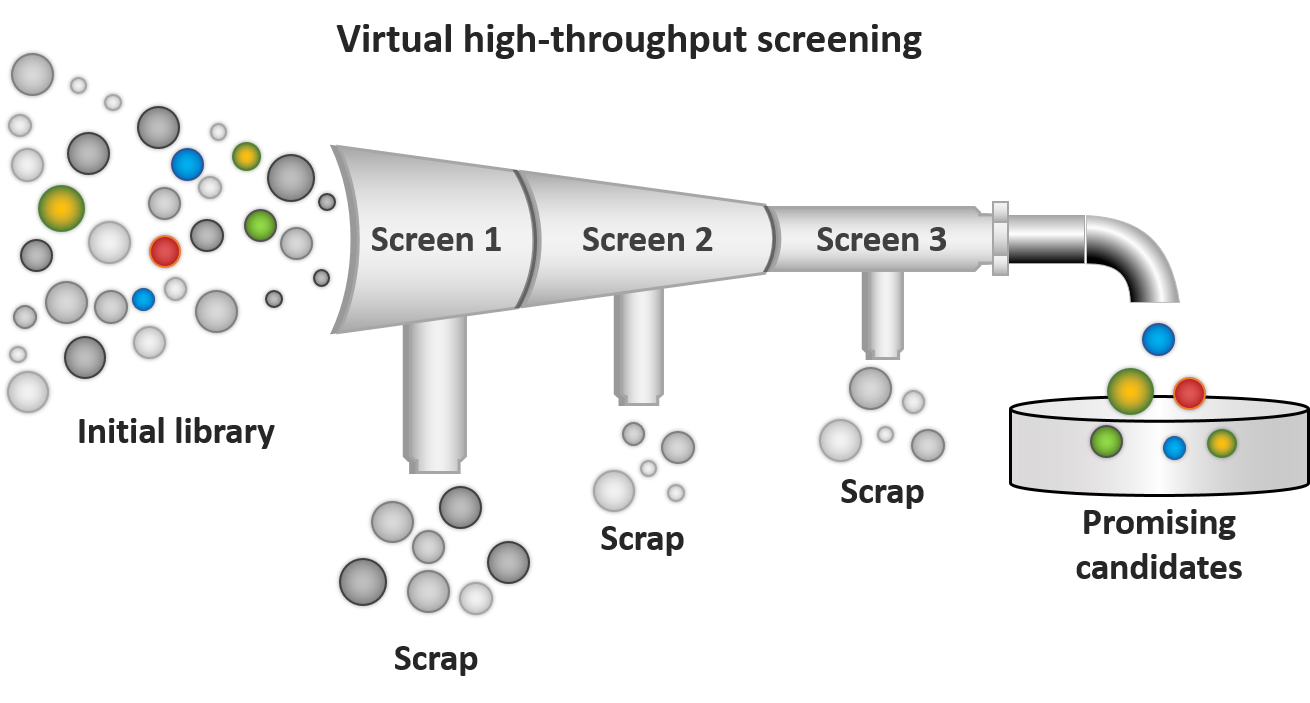
\includegraphics[width=0.9\textwidth]{Chapter-4/Figures/screen_pipe.png}
	\caption{Schematic for the screening of a library of molecules to identify promising candidates. At every level of screening, a higher level of theory is applied while narrowing down the chemical space.} 
	\label{fig:screen_pipe} 
\end{figure}  

\begin{figure}[htbp]
	\centering
	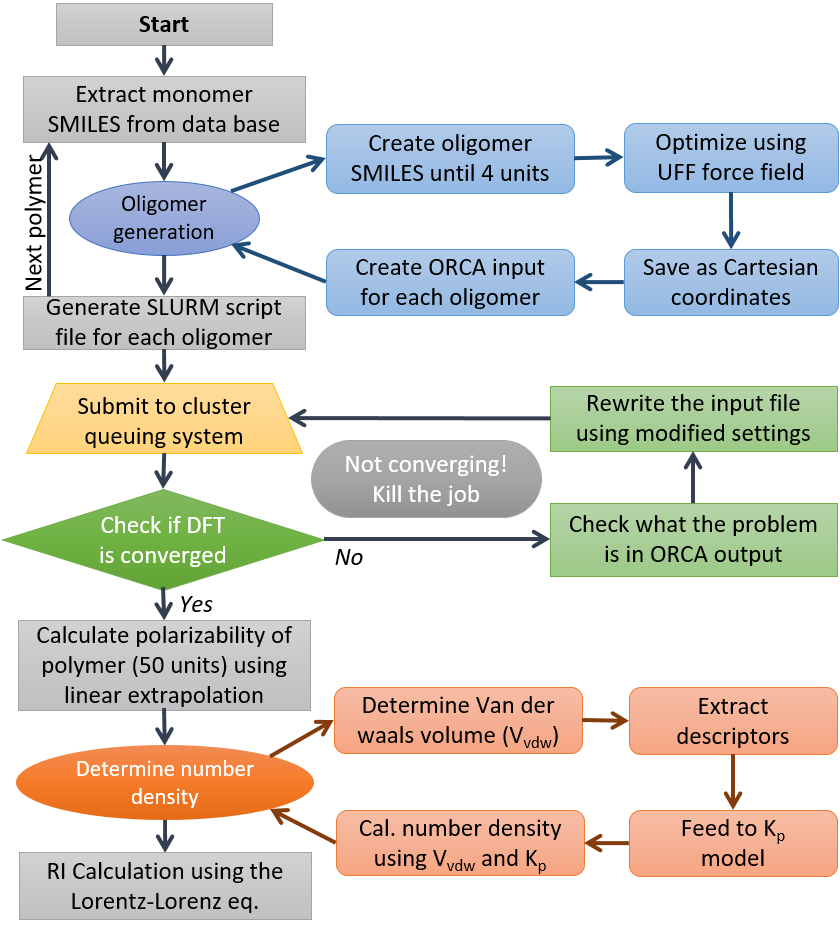
\includegraphics[width=0.7\textwidth]{Chapter-4/Figures/workflow.png}
	\caption{Work-flow implemented for the automation of polarizability values of candidate libraries.} 
	\label{fig:workflow} 
\end{figure}  


\subsection{Database Infrastructure}
\label{subsec:chembddb}
The use of modern database technology is of particular importance in the context of data-intensive research. Despite their great utility and despite being essential for projects that accumulate large data sets, databases are still rarely featured in chemical research. Our group is developing the \chembddb\ code to simplify and streamline the use of databases and thus make them more accessible to non-expert users in the chemistry community. \chembddb\ provides an automated database setup, a data model template that can readily be customized, and the necessary tools to access and manipulate the database. 
As in \chemhtps\ , we have been developing the corresponding workflows by abstracting our experience from real-life application projects with flexibility and reusability in mind. All the data generated from the virtual high-throughput screening of high RI polymers is incorporated into a database using \chembddb. Screenshots of the database are shown in Fig.\ \ref{fig:chembddb_screenshot}, which were provided by Shirish Sivaraj. 

Developers of \chembddb\ are Aditya Sonpal, Shirish Sivaraj and Supriya Agrawal. 

\begin{figure}[htbp]
	\centering
	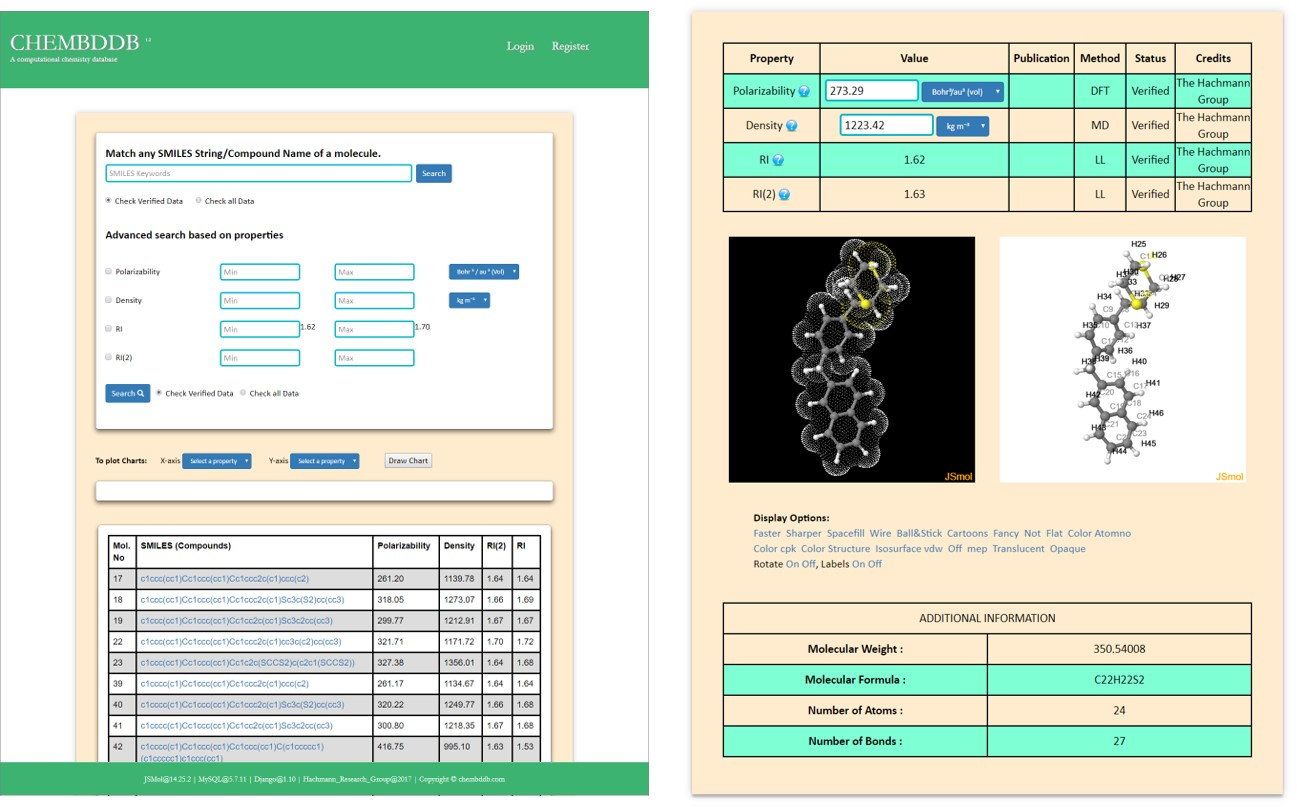
\includegraphics[width=1.0\textwidth]{Chapter-4/Figures/ChemBDDB_screeshot.jpg}
	\caption{Screenshots from the HRIP database.} 
	\label{fig:chembddb_screenshot} 
\end{figure}  

\subsection{Data Analysis, Mining, and Modeling Infrastructure}
\label{subsec:chemml}
We have been developing the \chemml\ program suite to establish data analysis, mining, and modeling capabilities that allow us to apply state-of-the-art machine learning and informatics methodology to chemical and materials data sets. \chemml 's principal tasks are the creation of predictive regression models and chemical pattern recognition/classification \cite{Kowalski1972}.

% introduce data-driven research; point to MGI and other high-profile initiatives for support of promise 
The resulting mapping functions (\ie  data-derived prediction models) are usually much easier to evaluate than physical models (\eg  the Schr\"odinger equation), so using them allows us to dramatically accelerate the characterization of chemical systems and it thus enables the hyperscreening of chemical space. 
A typical \chemml\ workflow encompasses a number of distinct steps that can be categorized in six main tasks: (1) input/output, (2) preprocessing, (3) learning, (4) validation, (5) evaluation, and (6) visualization. 

\chemml\ provides facilities for all these tasks \via\ classes of methods. These are either accessed from advanced third-party libraries and stand-alone programs (\eg  scikit-learn \cite{Pedregosa2011a}, Tensorflow \cite{tensorflow2015-whitepaper}, Keras \cite{chollet2015keras}, Dragon \cite{Taletesrl2011}, OpenBabel \cite{O'Boyle2011}, RDKit \cite{RDKit}), if these represent the state of the art for certain tasks, or from \chemmllib\ where we compile our new/original contributions as well as existing methods that are not otherwise accessible.  
The feature representation and the machine learning approach are two particularly important aspects in the generation of data-derived models, and they determine a model's predictive performance. 
\chemml\ can readily call many standard machine learning (as well as preprocessing and visualization) methods. Examples of available algorithms include multivariate regression \cite{ChristopherMBishop}, support vector machines \cite{Muller2001}, artificial neural networks \cite{Manzhos2006,Behler2007}, and deep learning \cite{dahl2015deep}. 
To support chemistry applications, \chemml\ interfaces the core learning algorithms with domain-specific tools, such as the feature space of molecular descriptors \cite{Todeschini2000,Sykora2008}, topological fingerprints \cite{Nilakantan1987,OBoyle2016c}, or more recent developments such as the Coulomb matrix \cite{Rupp2012} and bag-of-bonds \cite{Hansen2015b} descriptors. These feature spaces are the abstract `basis set' in terms of which a machine learning model for a particular structure-property relationship is numerically expressed \cite{Ramakrishnan2017}, and \chemml\ provides a comprehensive collection of existing schemes. While our current work focuses on supervised learning, we plan to broaden our scope to unsupervised and reinforcement learning in the future. 

The primary developer of \chemml\ is Mojtaba Haghighatlari. Other contributors include Ramachandran Subramanian, Bhargava Urala, Gaurav Vishwakarma, Aditya Sonpal, Po-Han Chen, and Srirangaraj Setlur.



\section{Software Ecosystem}
\label{subsec:ecosystem}
The four program packages discussed in the previous sections (\chemlg, \chemhtps, \chembddb, and \chemml) are loosely connected, \ie  they can either be employed as a comprehensive unit (see Fig.\ \ref{fig:ecosystem}), or in combination with drop-in replacements (\eg  with a different library generator or a custom database engine), or as standalone applications. 
The development work on our software ecosystem includes conceptual work, the design and assessment of protocols and workflows, the formulation of guidelines and best practices, and the implementation of both glue code and new methods. 
The key cyberinfrastructure challenges include the robust abstraction of workflows for general-purpose applications, scaling issues (\eg  associated with expensive data generation and the combinatorial nature of chemical space), code sustainability, as well as platform and distribution issues. While we emphasize black-box automation to reach non-expert users, we allow full customization of all settings (in particular in \chemml ). We continually extend and refine the features and capabilities of all four codes. These improvements are driven by feedback from application projects both inside and outside our group (cf.\ Sec.\ \ref{subsec:chemlg_app}). This input from different real-world application problems is a key to making this cyberinfrastructure as resourceful as possible. All codes are open and freely shared with the community under 3-clause BSD license \cite{Afzal2018b,Afzal2018c,Shirish2018,Haghighatlari2017}. All the repositories on GitHub are maintained by Hachmann Group. 

There are a number of exciting, high-profile software development efforts along similar lines by others in the field (\eg  \cite{Gunter2012,Ward2016}). 
% TODO: add better Materials Project reference and work by Kristin Persson; Open Chemistry
However, despite great popular demand, there is currently no cyberinfrastructure for data-driven \insilico\ research that is accessible to the community, applicable to a wide range of chemical problems, and that offers a level of comprehensiveness, automation, and integration comparable to that of modern computational chemistry program packages. Our contribution pursues this niche, which stands out in its scope and prospective utility.    

\section{Conclusions}

\label{sec:conclusions4}

The developed massively parallel generator, \chemlg, and the program suite for automated, virtual high-throughput screening studies, \chemhtps, offers a multitude of options to customize and restrict the scope of the enumerated chemical space and thus tailor it for the demands of specific applications. We incorporate genetic algorithms into the framework to streamline the non-combinatorial exploration of chemical space. Genetic algorithms have shown to be effective in optimizing chemical structures and generating useful compounds for different target applications. The parallel implementation of these codes and their integration with HPC systems allows us to create and setup screening of millions of molecular candidates in few seconds to minutes. 
	 
%Our software ecosystem recognizes the great opportunities that are arising with the shift towards a data-driven \insilico\ research paradigm in chemistry, materials science, and the corresponding engineering disciplines. 
%It focuses on delivering and deploying a cyberinfrastructure that is filling a distinct infrastructure gap and on building foundations that make data-driven research a viable and widely accessible proposition for the chemistry community. 
%The template for our efforts is the rise of computational chemistry program packages over the past decades and the tremendous impact it has had on the role of modeling and simulation in contemporary chemical research. 
%Following this example, our research program aims to advance our capacity to tackle complex discovery and design challenges, and improve our understanding of the associated molecular systems.
%We have shown in real-life application projects that this approach indeed offers a path to overcoming some of the prevalent limitations of traditional trial-and-error approaches. 



\chapter{Accelerated Discovery of High-Refractive-Index Polyimides}

Polyimides have attracted much attention due to their exceptional thermal stability and ease of processability. Further, polyimides possess mechanical stability, good flexibility, flame resistance, radiation resistance and low dielectric constant, thus holding great promises for various applications.  However, these polymers have low refractive index (RI) values which limit their use in optical and optoelectronic applications. In this study, we present a computational approach to discover novel high RI polyimides (PI). We use an RI prediction model, developed in our previous work, to calculate the RI values of large candidate library of PIs, created from building blocks provided by our experimental collaborators. To accelerate the development process and effectively screen the relevant high RI PIs, we cast the RI model into \chemhtps: a high-throughput screening, materials informatics, and rational design framework software developed in our group. We prove that \chemhtps\ is promising for rapidly identifying PIs with exceptionally high RI values. We explore various paths that introduce highly polarizable moieties into PI backbones to increase RI. We also identify monomer building blocks within PIs that are prevalent in high RI PIs, and discover building block combinations that result in the same. Additionally, we provide insights into the relationship between the structure and the RI values of polyimides, thus allowing us to target most promising candidates. We thank Prof. Cheng for providing us with building blocks and generation rules for synthetic feasibility. We acknowledge Sai Prasad Ganesh for his contributions in this work. He contributed to understanding the dependence of the polarizability on the geometry of molecules.  


\section{Introduction}
\label{sec:introduction5}

%Addressing the need for discovery of high RI polymers
Organic small molecules, oligomers, and polymers are emerging materials that feature many attractive properties compared to conventional inorganic materials. Devices made out of organic polymers are generally flexible, mechanically stable on impact, light-weight, and inexpensive to produce. This has led to increased efforts in utilizing these compounds in many different application domains, including optic and optoelectronic devices such as organic light-emitting diodes \cite{ThejoKalyani2012}, complementary metal oxide semiconductor \cite{Nakagawa2010},  photovoltaics \cite{Hachmann2011}, field-effect transistors \cite{Sirringhaus2009}, displays, and image sensors \cite{Angione2011}, in which they can be introduced \insitu\ as microlenses, waveguides, microresonators, interferometers, anti-reflective coatings, optical adhesives, and substrates. However, most of these applications require materials with a refractive index (RI) greater than 1.7 or larger, while typical carbon-based polymers only exhibit values in the range of 1.3-1.5 \cite{Liu2009}. This provides an incentive to discover or design new high-refractive index polymers (HRIPs) for the aforementioned applications. As the properties of organic polymers can be tailored by controlling their molecular structure, they are a prime example for a rational design target.

%Polyimides properties leading to a promising candidate for optoelectronic devices
In recent years, polyimides (PIs) have been shown to have favorable electronic and mechanical properties that could form potential HRIP candidates. Despite showing inherently low RI values leading to a lack of present applicability, PIs have other attractive properties \citep{Mathews2007,Chang2006}.  
PIs are strong potential candidates due to their exceptional thermal stability, and ease of processability \citep{Duesselberg2011,Liu2007a,Higashihara2015}. These properties are complemented by their favorable mechanical stability, flexibility, flame resistance, radiation resistance and their sufficiently high molecular polarizability: properties which would allow for potential use in optoelectronics \citep{Mittal2013,Barikani2000}.

%PI’s poor optical properties, especially RI, limiting its use in these devices
As previously mentioned, the optical properties of PIs are significantly inferior compared to conventional metal oxides currently used in optical and optoelectronic devices \citep{Butnaru2013,Liu2009}. However, PI optical properties can be improved upon by several methods \citep{Fukuzaki2010,Liu2008b,Sydlik2011,Terraza2008,Carter2001}. One such technique is to control the chemical structure of PIs to allow for precise tuning of optical properties, in particular to increase their RI values \citep{Liu2007a,Terraza2008,Yu1995,You2008}. In our study, we present a computational approach to study the RI of PIs and explore techniques that introduce highly polarizable moieties into polyimides framework to create a new class of high RI PIs. 

%Although, addition of some highly polarizable moieties might result in the discoloration of the PI material \cite{Barikani2000}. (Need more information on this, or remove it)

%Recent empirical approaches in increasing PI RI values by introducing different functional groups
Typically, HRIPs exist in the form of aromatic polyamides, and aromatic heterocyclic ring polymers, and certain conjugated aromatic polymers. However, these HRIPs struggle when it comes to optical implementation due to their large optical dispersion and large birefringence. The large birefringence is caused due to their aromatic, and conjugated pi-electron structures, which leads to poor transparency and coloration. The addition of highly polarizable moieties, which do not have significant pi-electron conjugation, can aid in increasing the RI of polymers. For example, small aromatic rings, halogen atoms, metals and particularly sulfur atoms have shown to be promising for this purpose \citep{Tsai2016,Kobayashi1998,Liu2007a,Sawada1998}. Previous experimental studies have demonstrated the ability of sulfur infused PIs to overcome potential unfavorable properties. In particular, high thermal stability, a low birefringence, an optical transparency in the visible light region, and high RI values have been demonstrated. In 2007, Ueda \textit{et. al.} developed PI films which were shown to have high RI values, but had unfavorably high birefringence in the range of 0.012 \cite{Liu2007b}. However, in recent years, experimental work has shown improvement in terms of birefringence and RI, with RI in the range of 1.76 and birefringence of 0.009 attained in particular, due to the high sulfur content of the PIs \cite{Yeo2015}. These encouraging results have led to our study being primarily concerned with sulfur incorporated PIs, and in doing so, generate a new class of HRIPs that does away with the technical limits of existing HRIPs.

%Number of possible options to create PI with potentially high RI values. However, there is limitation in what empirical studies could attain. With some input from empirical expertise, the computational studies could get the right direction to focus in the large chemical space.
Most of the PIs developed for high RI applications are based on the intuition of empirical observations. Therefore, there is a high possibility that there are potential HRIP candidates that are not studied experimentally simply because there are too many possible candidates to be feasibly studied. This motivation has led to our approach in generating a large library of promising PI candidates created by our molecular library generator. The library generator operates based on combinatorial linking, which could possibly to lead to an astronomical number of candidates beyond the scope of affordable computational studies. To counteract this, we narrowed the candidates generated from the library based on keen observations from past research and generation rules based on the input provided from our experimental collaborators. We created our PI library by casting these rules into the molecular library generator. We used our RI prediction model to evaluate the RI values of generated PI candidates \cite{Afzal2018a}.

%Accelerating the process of PI by using the RI protocol and in-house virtual high throughput screening framework. 
To facilitate RI evaluation of our large pool of candidates in a timely manner we use our virtual high-throughput screening framework, \chemhtps\ \cite{Afzal2018c}., that draws inspiration from The Harvard Clean Energy Project, which was successfully screened millions of organic molecules for photovoltaic applications \citep{Hachmann2011,Hachmann2014,Olivares-Amaya2011}. \chemhtps\ creates inputs, executes and monitors the calculations, parses and assesses the results, extracts and post-processes the information of interest, inserts the key outcomes into the project database, and archives all other data. Using this \insilico\ methodology we created a large number of novel PI candidates and characterized these candidates at a fraction of the time and cost of traditional studies.

\section{Methods}
\label{sec:methods5}
%1.	Refer the protocol to determine the polarizability and RI of polymers from previous paper
In our previous work, we developed a model for the prediction of RI of polymers, which was validated against experimental RI values of 112 non-conjugated polymers \cite{Afzal2018a}.  The RI prediction model is based on a synergistic combination of \textit{first-principles} quantum chemistry calculations and data modeling. In this scheme, we calculate RI values using the Lorentz-Lorenz equation, which involves two critical parameters, the number density and the polarizability. We calculate the former using van der Waals volume and packing factor of the polymer, while for the polarizability calculations, we use \firstprinciples. 

%2.	Describing tools for automating the framework of RI calculation of polymers using different method
We developed a library of PIs using our molecular library generator, \chemlg\ \cite{Afzal2018b}. The library is based on 29 building blocks and bonding rules (see Fig. \ref{fig:Building_blocks}, which were selected based on the suggestions provided by our experimental collaborator, Cheng's group. Based on these generation rules, we created about 50 thousand and 230 thousand possible structures for $R_1$ and $R_2$, respectively. We saved the structures in the form of SMILES string along with a code which contains the information on the list of building blocks and connections that were used to make a particular structure. We subsequently used \chemhtps\ to screen the PI candidates to evaluate their RI values, and collected the data in our project database. 
%TODO - more information about the database or the supplementary information.

For each $R_1$ and $R_2$ SMILES, we generated fifty different 3D conformations using OpenBabel software \cite{OBoyle2011}. We selected the lowest energy conformation for each structure and further optimized the geometry using the universal force field (UFF) \cite{Rappe1992} as implemented in the OpenBabel software. We use a packing factor of 0.75 to calculate the number density of PIs, as previous experimental studies have shown that PIs typically have a packing factor of 0.75 \cite{Privalko1997}. 
%We do not use the previously developed data model for calculating the packing factor of PIs. This is because the PIs studied in this work are structurally different than the polymers that were used to build the data model. 
We calculated the van der Waals volumes using Slonimskii's method detailed in Ref.\ \cite{Slonimskii1970}. For the polarizability calculations, we use an all-electron, restricted DFT method with the PBE0 hybrid functional \cite{Adamo1999} in combination with the double-$\zeta$ quality def2-DZVP basis set by the Karlsruhe group \cite{Weigend2005}. We include Grimme's D3 correction \cite{Grimme2010} to account for dispersion interaction. We carried out all the quantum computations using the ORCA 3.0.2 quantum chemistry package \cite{Neese2012}. 


\begin{figure}[htbp] 
	\centering
	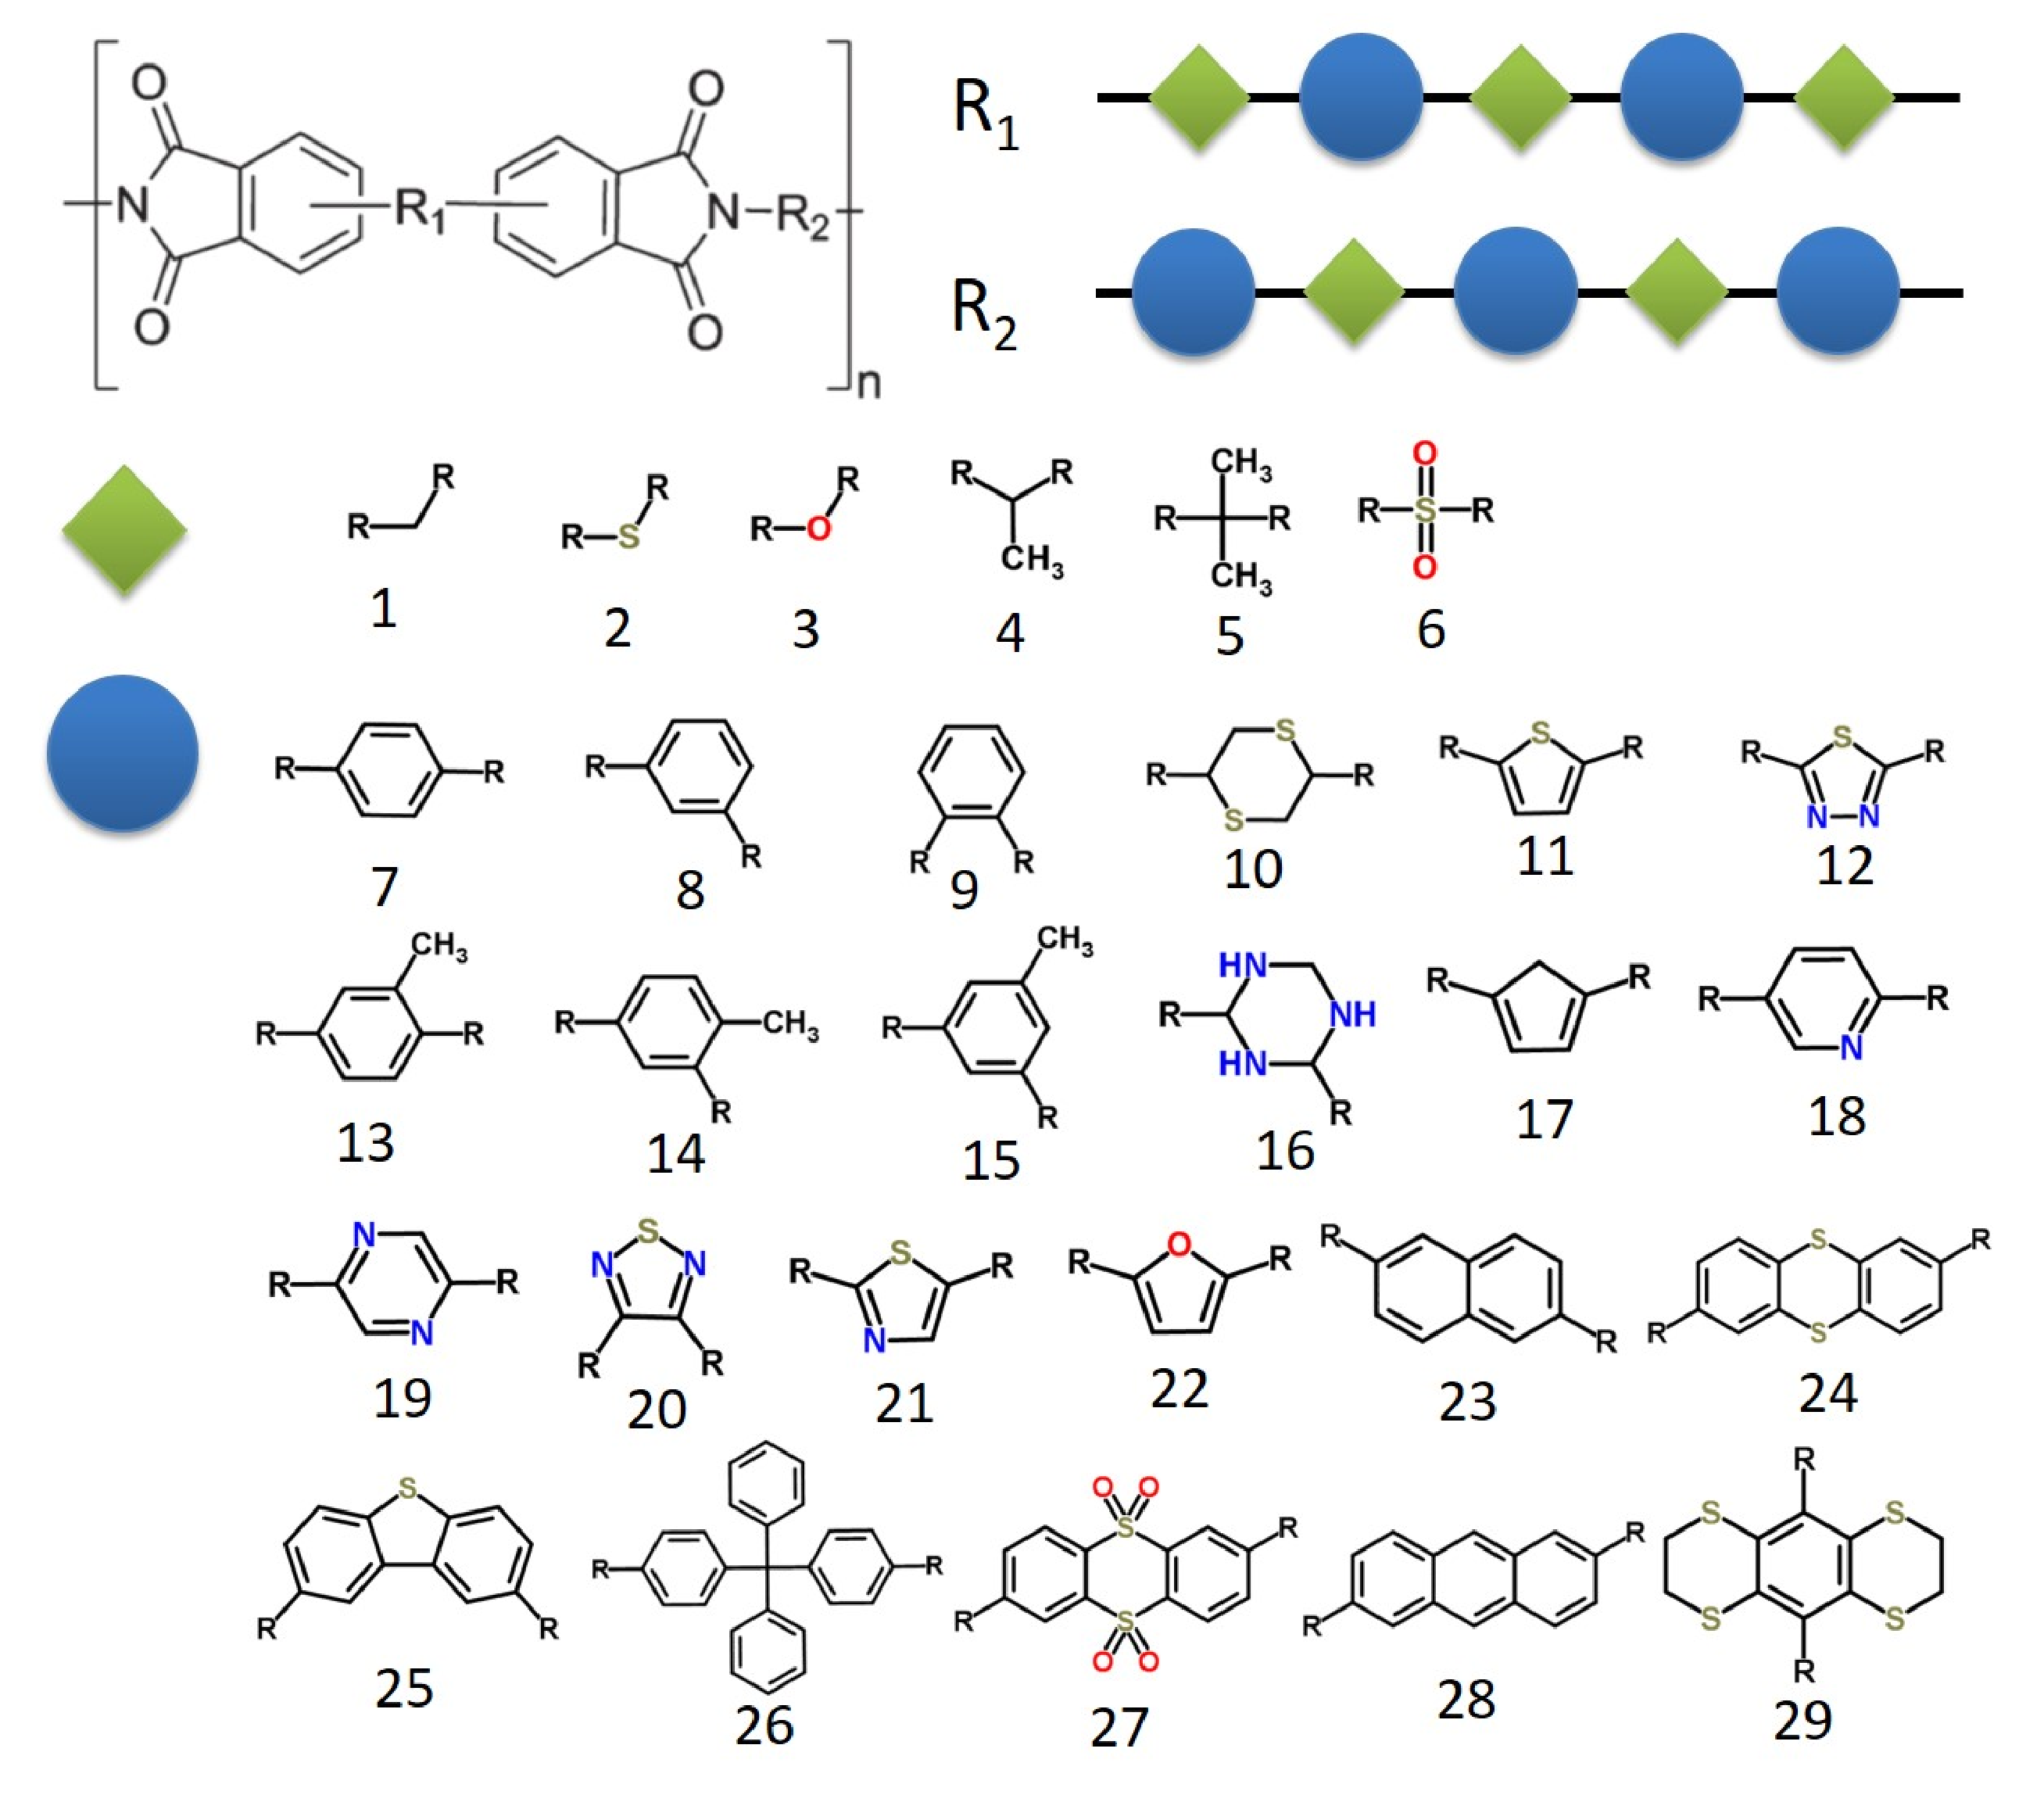
\includegraphics[width=0.744\textwidth]{Chapter-5/Figures/Building_blocks.eps}
	\caption{Building blocks used to create the library of PIs.} 
	\label{fig:Building_blocks} 
\end{figure} 

%3.	Describe the approach considered in understanding the structure-property relationships. 
In addition to identifying the best candidates from our high-throughput screening studies, we further analyze the collected data to understand structure-property relations. By applying Z-score analysis, we identify the building blocks that contribute the most to the RI values. We compute the Z-score ($Z_i$) of the candidates by
\[
Z_i=\frac{k-n\frac{K}{N} }{\sigma},\ \sigma=\left [ \frac{nK}{N}\times \left ( \frac{N-K}{N} \right )\times \left ( \frac{N-n}{N-1} \right )\right ]^{\frac{1}{2}}
\]
where $N$ is the total number of molecules, $n$ is the subset of molecules that are considered, $K$ number of occurrences of building block $i$ in $N$ molecules and the $k$ is the occurrences of building block $i$ in $n$ subset. We perform similar calculations to calculate the Z-score of the building block connections to identify the synergistic combinations that lead to the high RI values. 

\section{Results and Discussion}
\label{sec:results_discussion5}

%1.	Start with the contour plot for pol and density. Explain the way to obtain high RI value candidates.
According to the Lorentz-Lorenz equation, the RI of a material is dependent on its polarizability and number density. Using our previous studies conducted on a library of 112 non-conjugated polymers \cite{Afzal2018a}, we generated a contour plot to elucidate the relationship between the polarizability and the Number density (see Fig. \ref{fig:Den_pol_contour}). The contour plot demonstrates an inverse proportionality relationship between the number density and the polarizability. Our preferable high RI region happens when both the polarizability and number density are sufficiently high. However, there is a tendency for the number density to be low in highly polarizable materials. Therefore, in order to attain desirable optical properties, it is necessary to maximize both these parameters at the same time. One approach could be to restrict the compound space in a constant number density region and explore highly polarizable compounds in that region. Going forward with this logic, we choose the structure of PI as shown in Fig. \ref{fig:Building_blocks}. Given that the densities of these PIs are fairly similar, we can now search for highly polarizable PI candidates \cite{Privalko1997}. 


\begin{figure}[htbp] 
	\centering
	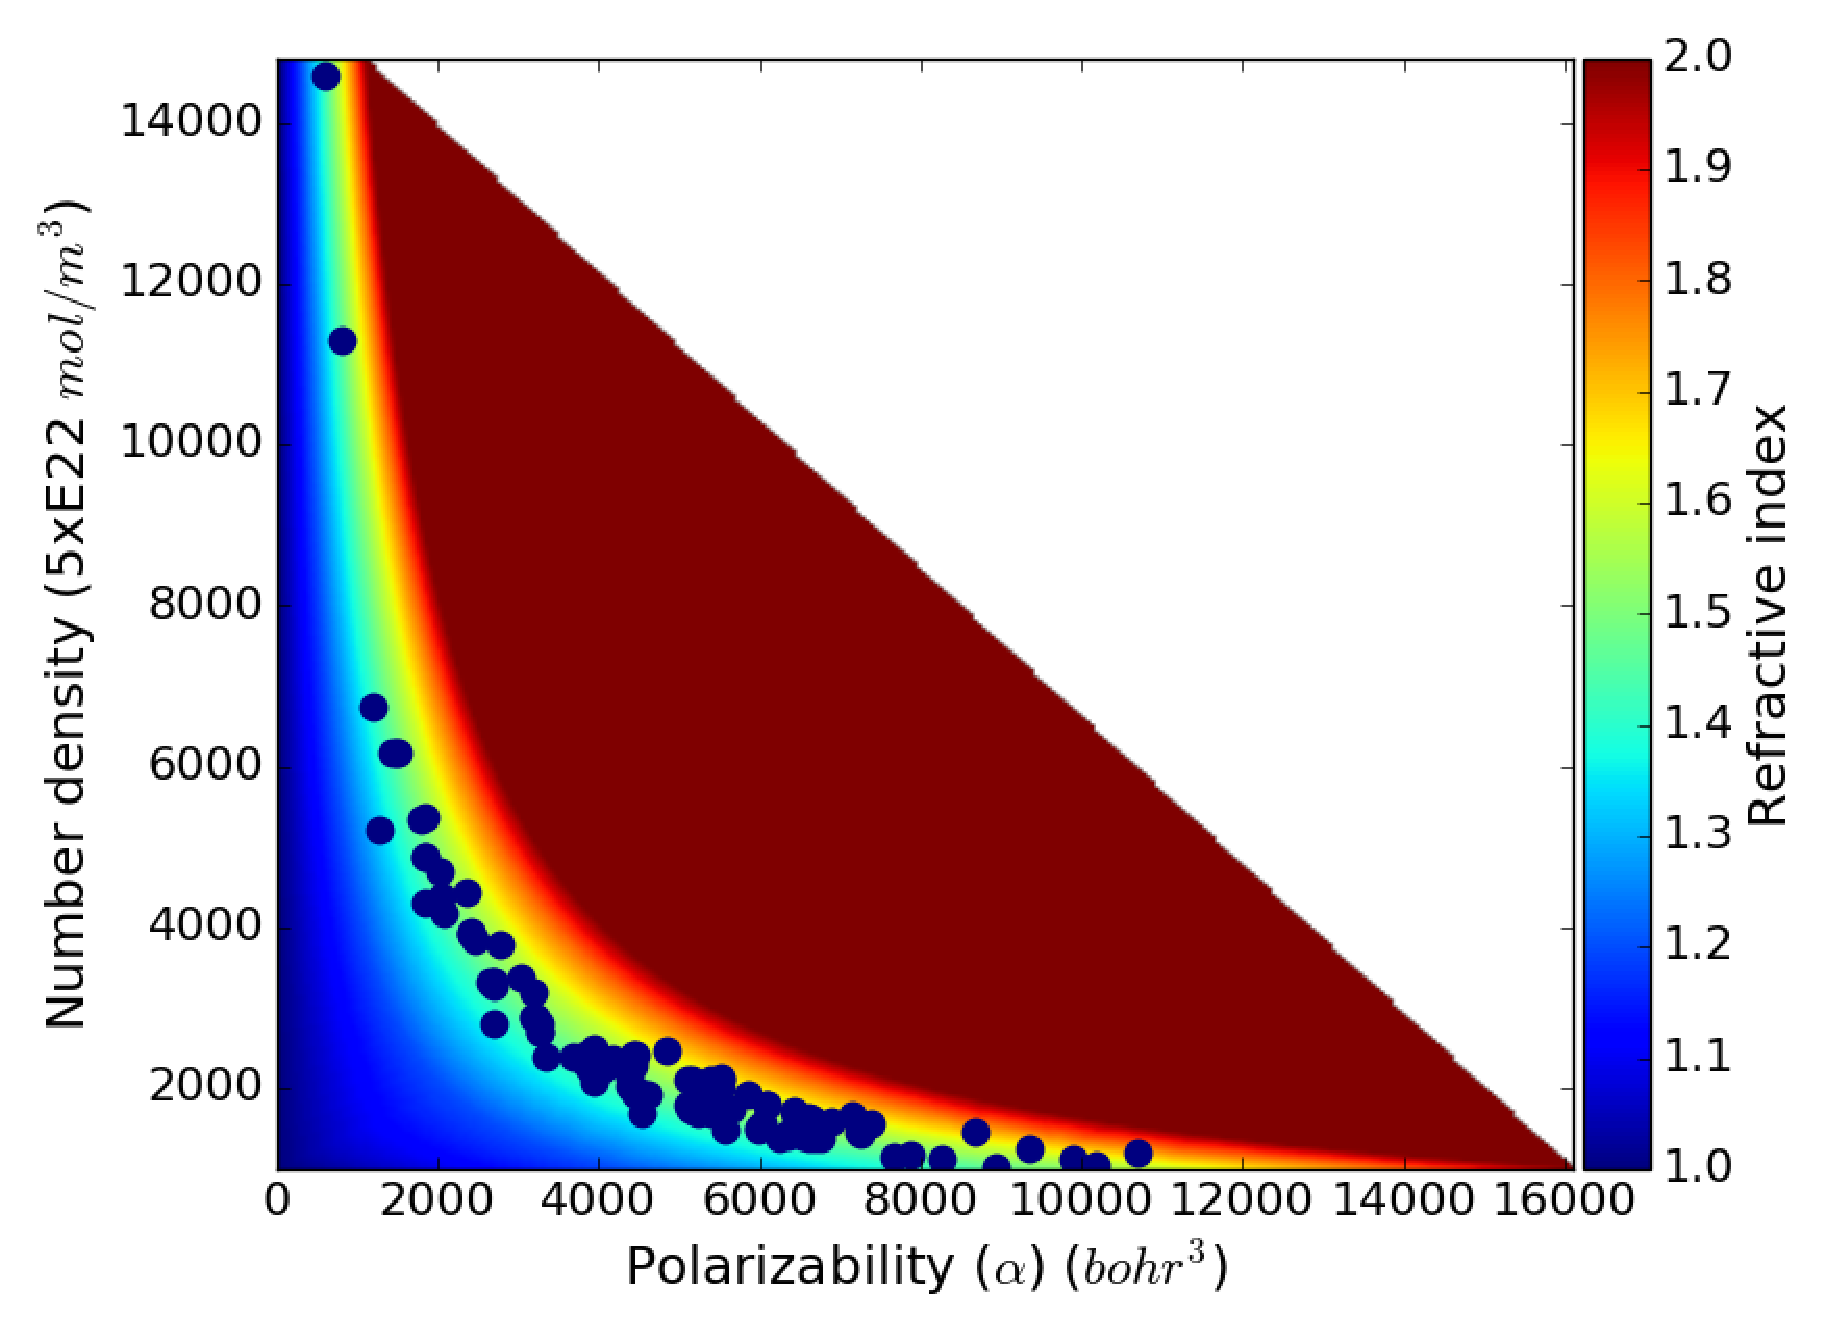
\includegraphics[width=0.744\textwidth]{Chapter-5/Figures/Den_pol_contour.eps}
	\caption{Contour plot representing the dependence of RI on the polarizability and number density. Blue dots refer to the 112 polymers used to develop RI model.} 
	\label{fig:Den_pol_contour} 
\end{figure}  

%2.	RI value of about 10 PI polymers and compare with the experimental values.

\newcolumntype{C}[1]{>{\centering\arraybackslash}m{#1}}

\begin{table}[htbp]
	\centering
	\caption{Comparison of RI values from RI prediction model with the experimental values of 10 PI candidates} \label{tab:comparison}
	\renewcommand{\arraystretch}{1.5}% Spread rows out...
	\label{Table_comp}
	\begin{tabular}{>{\centering\bfseries}m{1in}|c| >{\centering}m{1in} >{\centering}m{1in} >{\centering\arraybackslash}m{1in}}
		%\begin{tabular}{|C{1.5cm}|c|C{1.6cm}|C{1.5cm}|C{1.5cm}|}
		\multicolumn{5}{l}{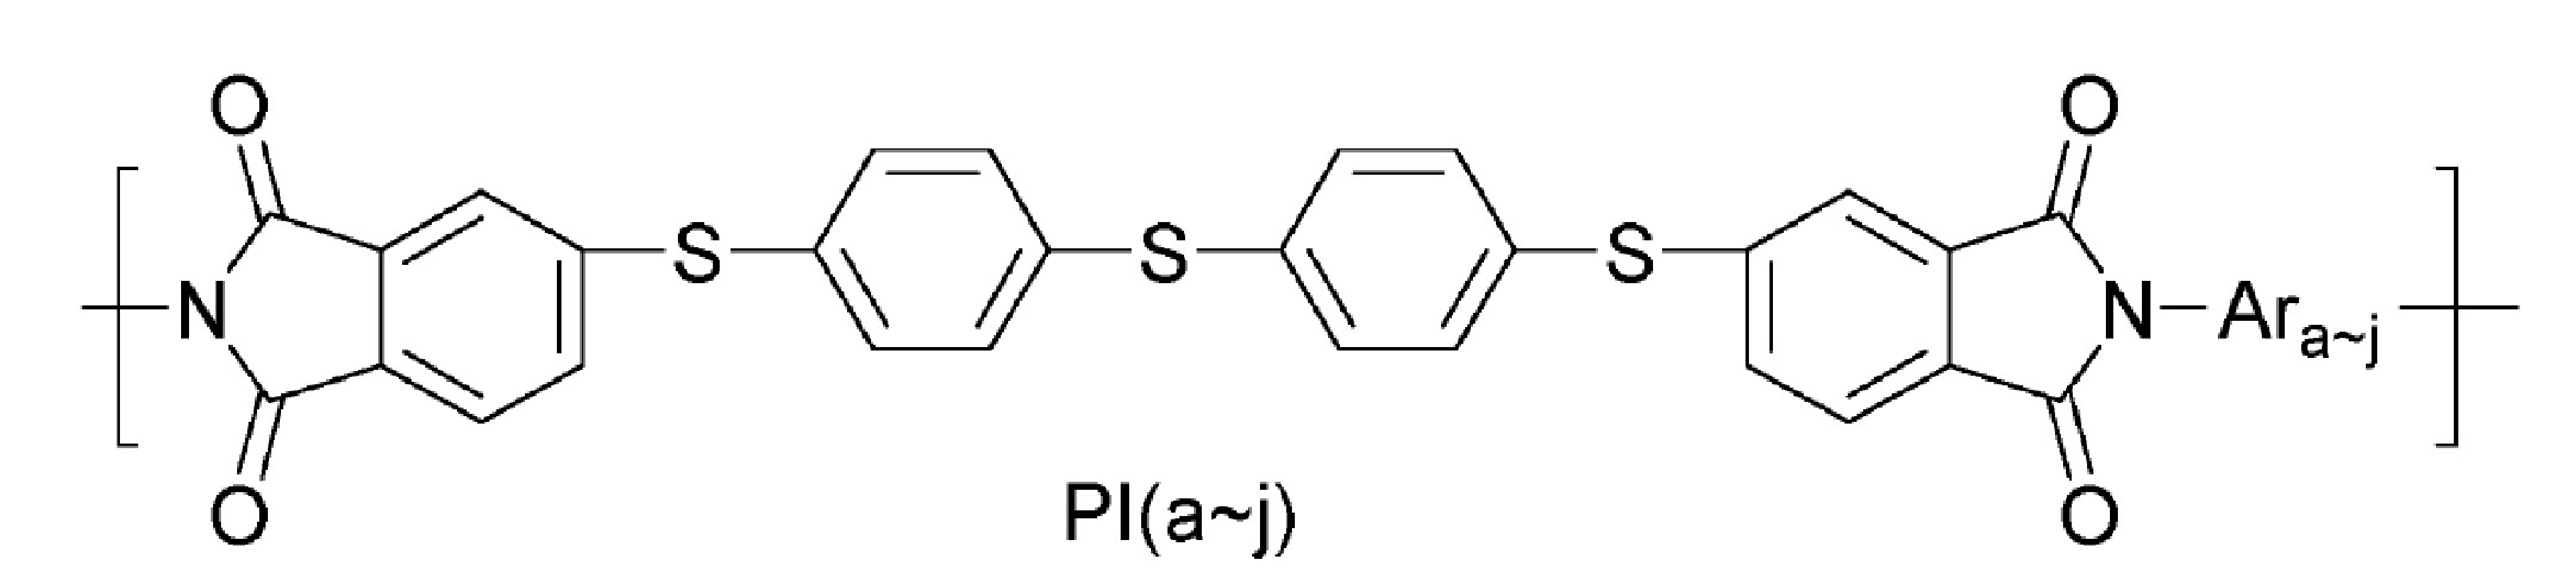
\includegraphics[width=0.5\textwidth]{Chapter-5/Figures/PI_strcutres/PI.eps}}      \\ \hline
		\multicolumn{1}{|C{1cm}|}{$\mathrm{Ar}_\mathrm{a-j}$} & \multicolumn{1}{c|}{Structure} & \multicolumn{1}{C{2.2cm}|}{Experiment value \cite{Liu2009}} & \multicolumn{1}{C{2cm}|}{Calculated value} & \multicolumn{1}{C{1.4cm}|}{Error}  \\ 
		\multicolumn{1}{|c|}{a}       & \multicolumn{1}{l|}{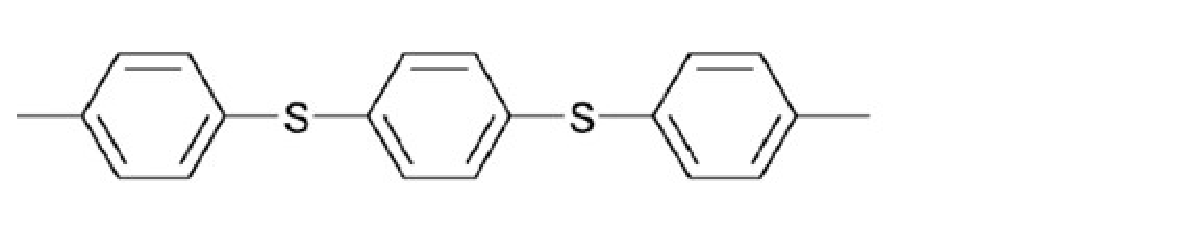
\includegraphics[width=0.4\textwidth]{Chapter-5/Figures/PI_strcutres/a.eps}}          & \multicolumn{1}{c|}{1.746}            & \multicolumn{1}{c|}{1.738}            & \multicolumn{1}{c|}{-0.008} \\ 
		\multicolumn{1}{|c|}{b}       & \multicolumn{1}{l|}{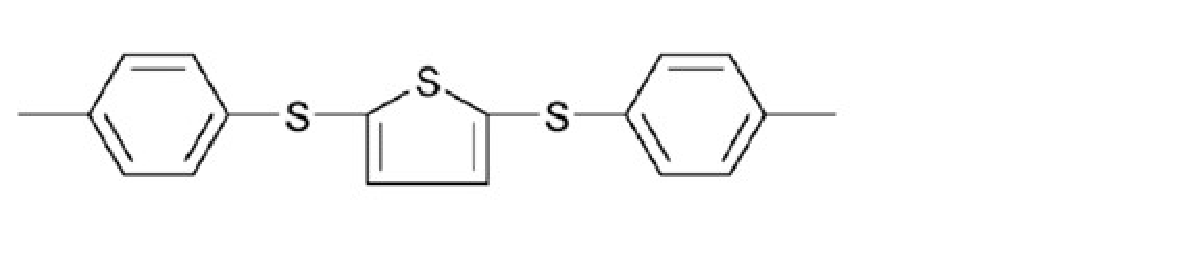
\includegraphics[width=0.4\textwidth]{Chapter-5/Figures/PI_strcutres/b.eps}}          & \multicolumn{1}{c|}{1.753}            & \multicolumn{1}{c|}{1.739}            & \multicolumn{1}{c|}{-0.013} \\ 
		\multicolumn{1}{|c|}{c}       & \multicolumn{1}{l|}{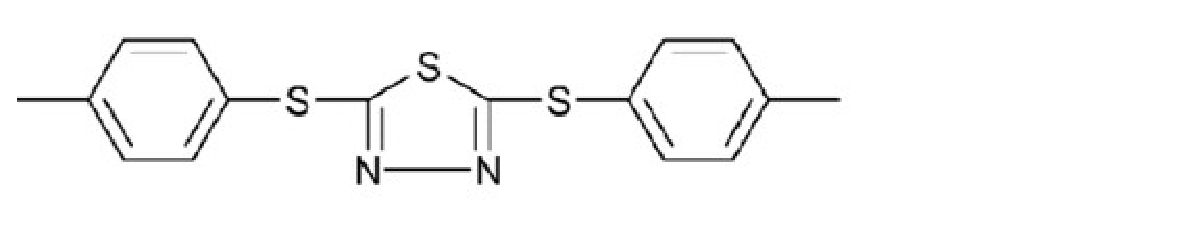
\includegraphics[width=0.4\textwidth]{Chapter-5/Figures/PI_strcutres/c.eps}}          & \multicolumn{1}{c|}{1.749}            & \multicolumn{1}{c|}{1.707}            & \multicolumn{1}{c|}{-0.042} \\ 
		\multicolumn{1}{|c|}{d}       & \multicolumn{1}{l|}{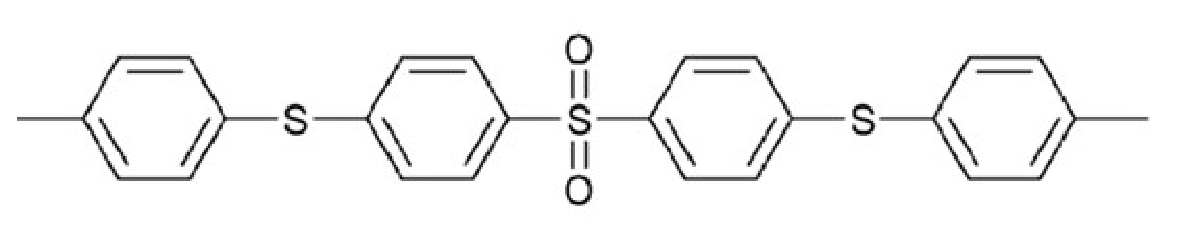
\includegraphics[width=0.4\textwidth]{Chapter-5/Figures/PI_strcutres/d.eps}}          & \multicolumn{1}{c|}{1.748}            & \multicolumn{1}{c|}{1.751}            & \multicolumn{1}{c|}{0.003}  \\ 
		\multicolumn{1}{|c|}{e}       & \multicolumn{1}{l|}{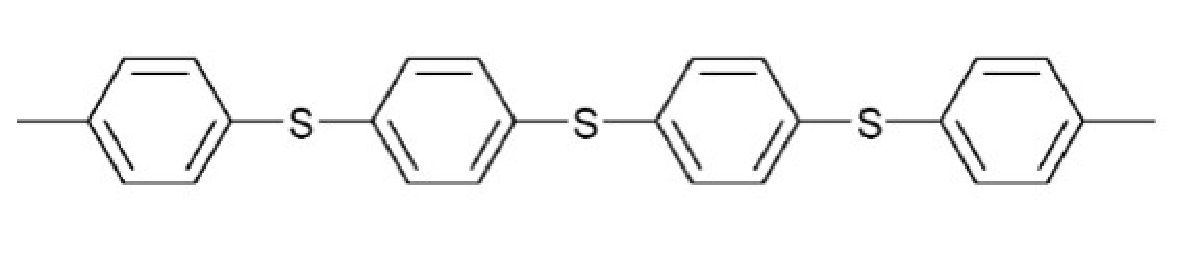
\includegraphics[width=0.4\textwidth]{Chapter-5/Figures/PI_strcutres/e.eps}}          & \multicolumn{1}{c|}{1.733}            & \multicolumn{1}{c|}{1.760}            & \multicolumn{1}{c|}{0.027}  \\ 
		\multicolumn{1}{|c|}{f}       & \multicolumn{1}{l|}{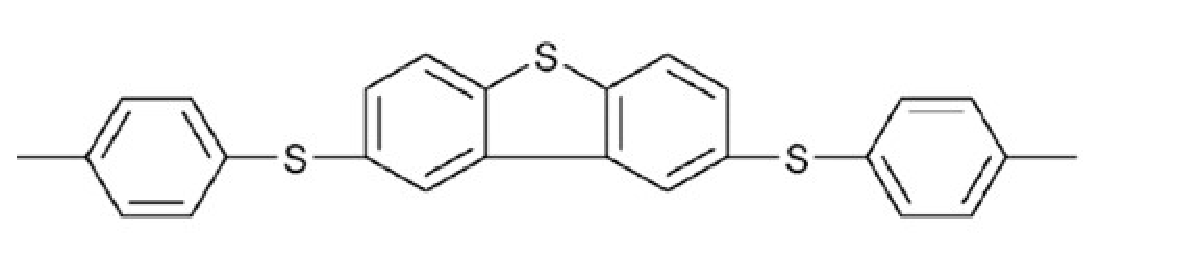
\includegraphics[width=0.4\textwidth]{Chapter-5/Figures/PI_strcutres/f.eps}}          & \multicolumn{1}{c|}{1.758}            & \multicolumn{1}{c|}{1.779}            & \multicolumn{1}{c|}{0.021}  \\ 
		\multicolumn{1}{|c|}{g}       & \multicolumn{1}{l|}{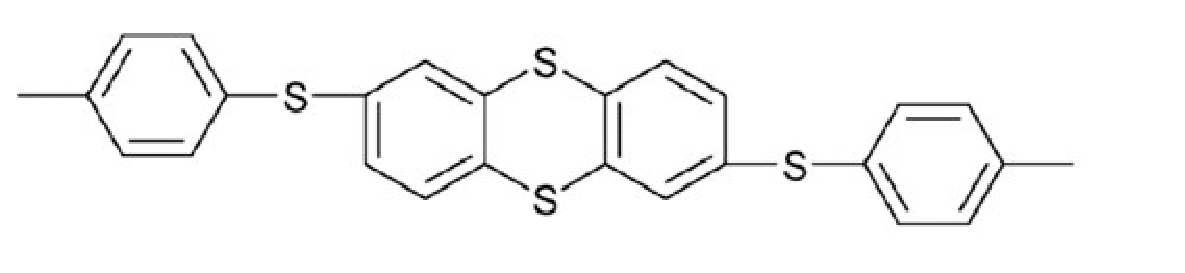
\includegraphics[width=0.4\textwidth]{Chapter-5/Figures/PI_strcutres/g.eps}}          & \multicolumn{1}{c|}{1.760}            & \multicolumn{1}{c|}{1.735}            & \multicolumn{1}{c|}{-0.025} \\ 
		\multicolumn{1}{|c|}{h}       & \multicolumn{1}{l|}{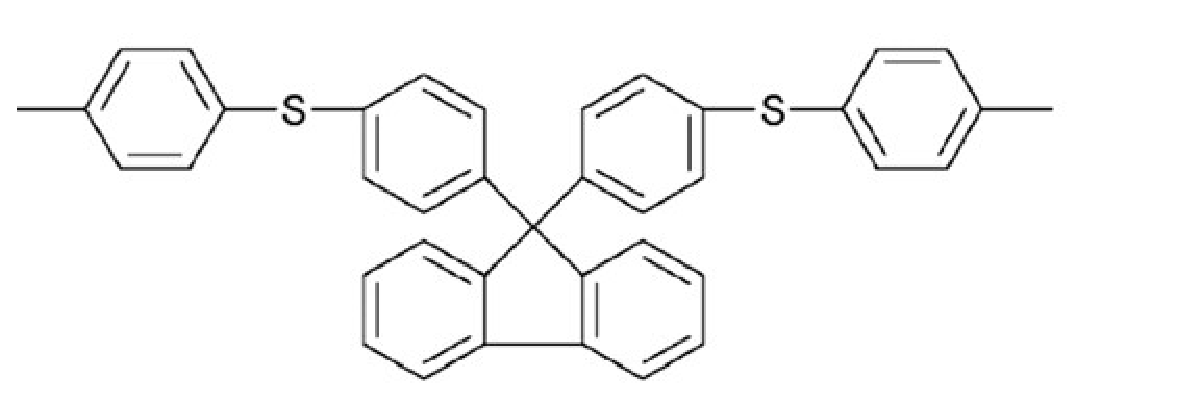
\includegraphics[width=0.4\textwidth]{Chapter-5/Figures/PI_strcutres/h.eps}}          & \multicolumn{1}{c|}{1.726}            & \multicolumn{1}{c|}{1.741}            & \multicolumn{1}{c|}{0.015}  \\ 
		\multicolumn{1}{|c|}{i}       & \multicolumn{1}{l|}{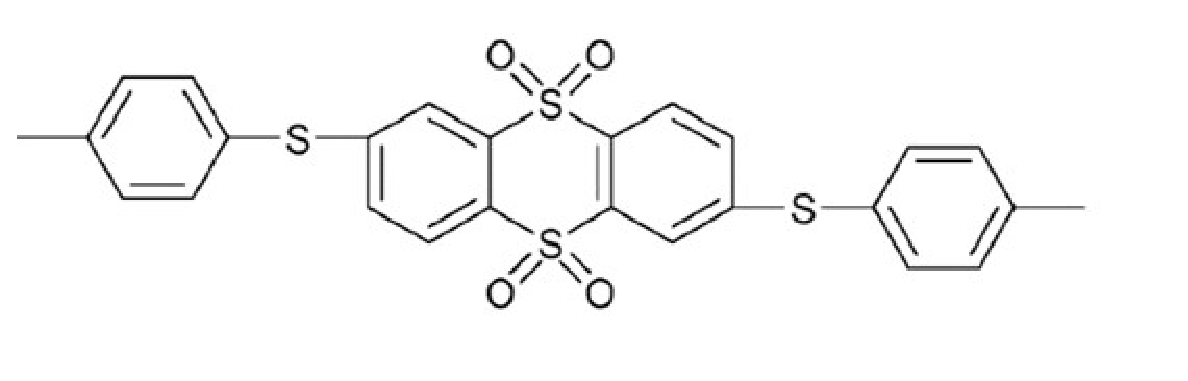
\includegraphics[width=0.4\textwidth]{Chapter-5/Figures/PI_strcutres/i.eps}}          & \multicolumn{1}{c|}{1.737}            & \multicolumn{1}{c|}{1.743}            & \multicolumn{1}{c|}{0.005}  \\ 
		\multicolumn{1}{|c|}{j}       & \multicolumn{1}{l|}{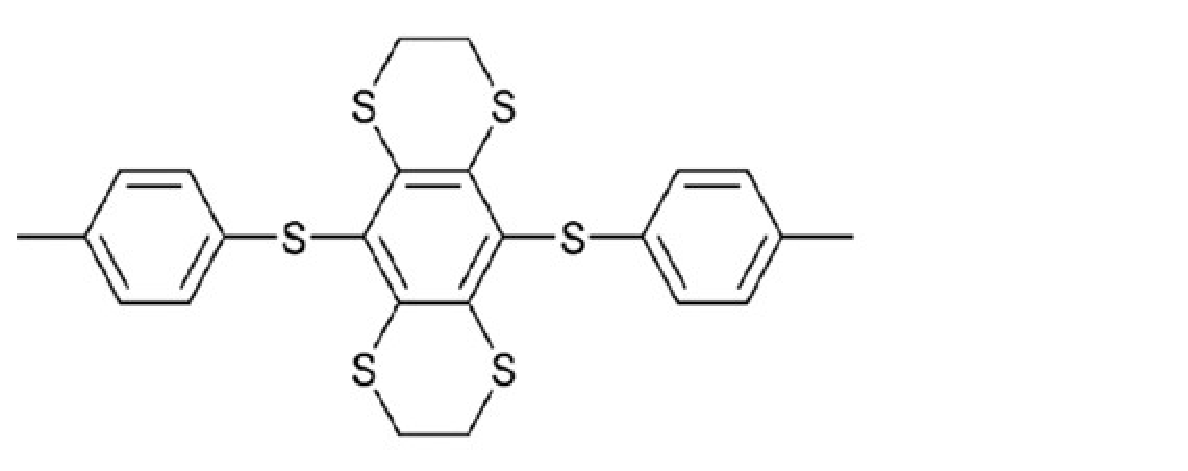
\includegraphics[width=0.4\textwidth]{Chapter-5/Figures/PI_strcutres/j.eps}}          & \multicolumn{1}{c|}{1.769}            & \multicolumn{1}{c|}{1.724}            & \multicolumn{1}{c|}{-0.045} \\ \hline
	\end{tabular}
\end{table}

As mentioned in the methods section, we calculate the RI of PIs using a model that involves the calculation of the polarizability and the number density values. We previously tested this model against 112 non-conjugated polymers, however, there were no PI candidates in this list. Therefore, to check the validity of our RI model on the PI structures, we compared the model with experimental RI values of 10 PIs shown in table \ref{Table_comp}. The RMSD of the model is 0.024, suggesting that our model is accurate for calculating the RI of PIs.

%3.	Explanation of the selection of building blocks and the process of creation of PI library. PI split into two segments, $R_1$ and $R_2$, and separately studied. X number of $R_1$ and Y number of $R_2$ were created based on generation rules. 
In search of high RI PIs, we created about 50 thousand and 220 thousand structures of $R_1$ and $R_2$, respectively, using 29 promising building blocks as shown in Fig. \ref{fig:Building_blocks}. Combining all these $R_1$ and $R_2$ structures to form PI could lead to a total of 11 billion PIs. However, virtual high-throughput screening of such an astronomical number of structures is not a viable option. Therefore, we narrowed down the number of possible PI candidates by picking the best of the $R_1$ and $R_2$ structures. We did so by computing the RI values of the individual $R_1$ and $R_2$ structures. After the screening of these structures, we developed the most promising PI candidates by combining the top $R_1$ and $R_2$ structure as shown in \ref{fig:Building_blocks}. 
%TODO - unclear, need a better explanation.

%4.	The RI values of the $R_1$ and $R_2$ library and the top candidates. The histogram of $R_2$.
In this paper, we discuss the results of $R_2$ structures. Figure \ref{fig:RI_hist} shows the RI distribution of $R_2$ structures. We observe a Gaussian type distribution for the RI values of $R_2$ structures. Most of the candidates have RI values between 1.5 and 1.7, which suggests that there is a strong possibility of obtaining molecules with such RI values using empirical approaches. However, using a computational approach, we we were able to find the outliers, i.e., the candidates with RI values greater than 1.7. 
%Using the developed RI prediction protocol and casting this protocol into the ChemHTPS framework, the most promising candidates for $R_1$ and $R_2$ structures were identified. 

\begin{figure}[htbp] 
	\centering
	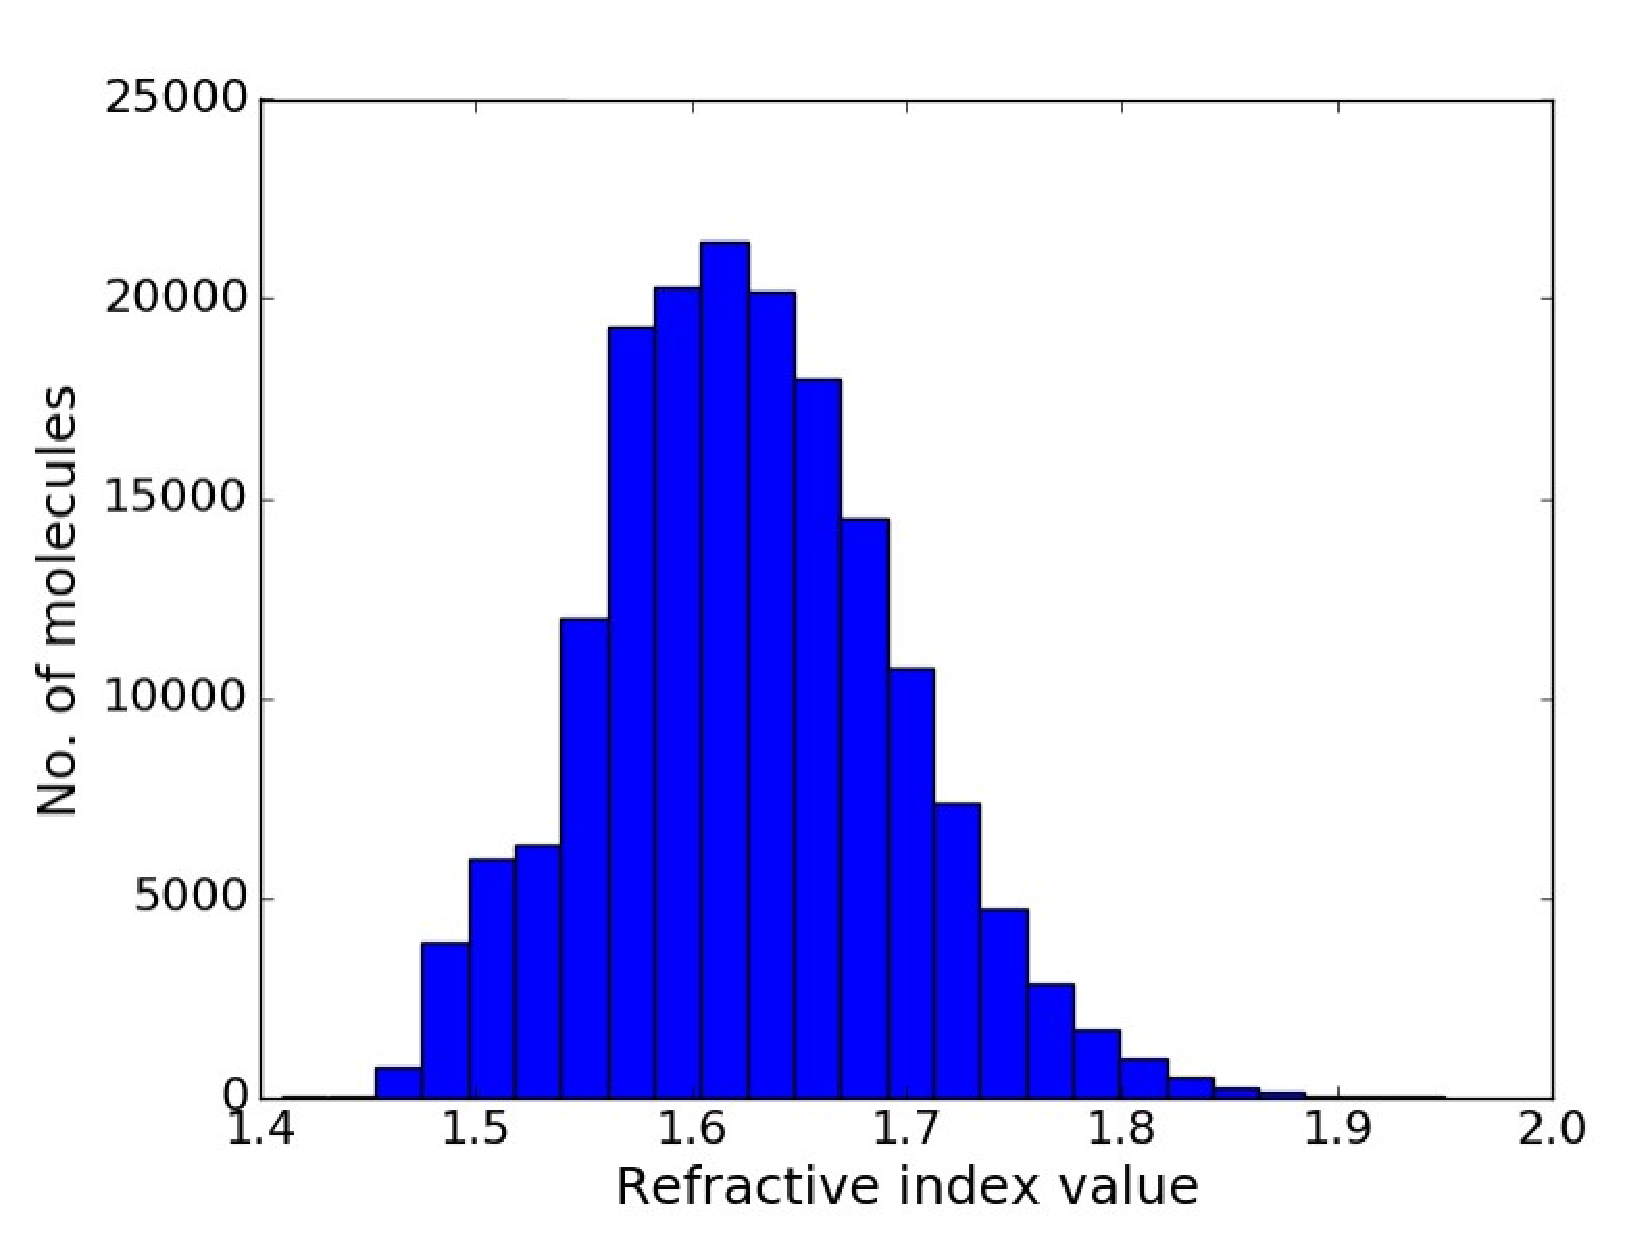
\includegraphics[width=0.700\textwidth]{Chapter-5/Figures/RI_histogram.eps}
	\caption{RI distribution of the $R_2$ structures} 
	\label{fig:RI_hist} 
\end{figure}  

%5.	Combining the best of $R_1$ and $R_2$ to form a full PI.
The top 100 structures of $R_1$ type and top 1000 structures of $R_2$ type are selected to form 100,000 PI monomers. We casted these PI structures into our HTPS framework to evaluate the RI values.
%TODO - need more information here.

%6.	Looking at the building blocks contribution
\begin{figure}[htbp] 
	\centering
	\includegraphics[width=0.700\textwidth]{Chapter-5/Figures/BB_avg_RI.eps}
	\caption{Average RI of the structures containing each building block in the top 10\% candidates of $R_2$. } 
	\label{fig:BB_avg_RI} 
\end{figure}  

\begin{figure}[htbp] 
	\centering
	\includegraphics[width=0.700\textwidth]{Chapter-5/Figures/BB_top_Z.eps}
	\caption{Z-score of each building block in the top 10\% candidates of $R_2$.} 
	\label{fig:BB_top_Z} 
\end{figure}  

Besides identifying the potential HRIP candidates, understanding the underlying structure-property relationships would enable us to discern candidates with optimal RI values. This would help us create a special subset of candidates for our experimental collaborators to further explore. To do so, we tried to recognize the contribution of each building block towards a targeted property to aid in identifying favorable synergies in building block combinations, with an aim to narrow our chemical search space. We decided to implement this into our studies by looking at two different scoring systems for the building blocks: i) the average RI value of the candidates which contain each building block and ii) the Z-score of each building block in the top candidates. We plotted the results obtained from the first method in Fig. \ref{fig:BB_avg_RI}, which presents the RI distribution of candidates containing a particular building block. Here, we found that for the $R_2$ structures, candidates containing building blocks 24, 25 and 28 have the highest RI values, while the candidates containing building blocks 17, 16 and 10 showed the lowest RI values. Figure \ref{fig:BB_top_Z} on the other hand shows the z-scores. This technique is favored as a higher z-score would mean a larger prevalence of a particular building block in a HRIP. In our case, we picked the top 10\% of candidates in terms of their RI values and evaluated the Z-scores of individual building blocks in this subset. The green color in the Fig. \ref{fig:BB_top_Z} represents a positive Z-score, whereas the red color represents a negative Z-score. This technique confirmed our results obtained by the first method as the Z-score values also suggest that the building blocks 24, 25 and 28 are the most promising for developing HRIPs.  

\begin{figure*}[htbp] 
	\centering
	\includegraphics[width=1.00\textwidth]{Chapter-5/Figures/All_BB_Z.eps}
	\caption{Z-score of each building block in all the $R_2$ structures. } 
	\label{fig:All_BB_Z} 
\end{figure*}  

The above Z-score analysis only gives the prevalence of building blocks in the top 10\% candidates, but not the remaining ones. In order to generate a more comprehensive structure-property relationship, we evaluated the Z-score of building blocks in the full spectrum of the library. For this, the library was divided into 10 subsets ordered by increasing RI values. We evaluated the Z-score of the building blocks in each of these 10 subsets and plotted them with increasing RI values (see Fig. \ref{fig:All_BB_Z}). The green color represents a positive Z-score and the red represents a negative Z-score. We observed certain trends in this plot:
\begin{enumerate}
	\item The Z-score of building blocks 2, 3, 23, 24, 25, 28 and 29 increase with increasing RI values.
	\item The Z-score of building blocks 4, 5, 10, 16, 17 and 22 decreases with increasing RI values.
	\item The Z-score of building blocks 7, 8, 9, 11, 13, 14, 15, 18, 26 and 27 change from a negative value to a positive value before becoming negative again.
	\item The building blocks 1, 6, 12,19, 20 and 21 do not show a clear trend, therefore appear to have less impact on the RI values 
\end{enumerate}

%#Using such analysis we could identify building blocks whose presence lead to a higher RI value. 

\begin{figure*}[htbp] 
	\centering
	\includegraphics[width=1.00\textwidth]{Chapter-5/Figures/Bonds_top_Z.eps}
	\caption{Z-score of building block combinations in the top 10\% candidates of $R_2$.} 
	\label{fig:Bonds_top_Z} 
\end{figure*}  

In addition to building blocks contribution to RI values, it is also important to note the impact of various building block combinations to further understand the structure-property relationship. Therefore, we calculated the Z-scores of all the possible building block combinations in the top candidates. Fig. \ref{fig:Bonds_top_Z} illustrates which building blocks combinations are promising for high RI polymers. The size of the circle in the plot represents the magnitude of the Z-score value. The green color of the circle indicates a positive Z-score, whereas the red circle indicates a negative value. Using this figure, we can see that the combination of building block 28 with blocks 2 and 3 occur very frequently in top candidates given by the large size of the circle. The combinations of building blocks 23, 24, 25 and 28 with building blocks 1, 2 and 3 appear to be promising for the creating HRIPs. 
%TODO - further discussion required

The above structure-property relationships demonstrate the best building blocks and the combinations of these building blocks which are highly promising in developing HRIPs. We will use these guiding principles to create the next generation of HRIPs, and further validate these candidates by synthesizing them and testing their RI values. The best candidates from this study are currently being synthesized by our experimental collaborators, which we will be publishing soon.
%TODO - check with Prof Cheng regarding the results. 

\section{Conclusions}
\label{sec:conclusions5}

We demonstrated the developed RI model is successful in calculating the RI values of polyimides. We successfully created a molecular library of 270,000 PIs from promising building blocks, suggested by our experimental collaborators. We identified the best candidates by screening the library using our virtual high-throughput screening framework. The screening study resulted in more than 2000 PIs with RI values greater than 1.8. In addition to identifying high RI candidates, we applied materials informatics and data mining techniques to understand the relationship between the molecular structure and the RI values. Using these techniques, we identified building blocks and combinations of building blocks that are prominent in the top RI candidates. The developed rational design framework is successful for the accelerated discovery of polyimides with exceptional RI values.



\chapter{Neural Networks for the Prediction of RI of 1.5 Million Organic Molecules}

One of the most important and non-trivial properties of these molecules is the molecular packing. The packing density of organic molecules is highly dependent on the molecular structure. Organic molecules with a targeted density can be achieved by controlling the chemical structure. We can understand more about the correlation between the molecular structure and packing density of molecules by studying a large number of molecular candidates. Using our in-house molecular generator, we generated a molecular library of 1.5 million small organic molecules. The most accurate way to evaluate the density of these molecules is by performing molecular dynamics (MD) simulations. Since MD simulations are computationally intensive, performing simulations for a large library of molecular candidates is not a viable option. Therefore, we selected hundred thousand molecules from the library and evaluated their density values. Using this data as training set, we developed an exceedingly efficient ($R^2$=0.98) neural network model to correlate molecular structural descriptors with their properties. Using this correlation, we were able to quickly compute the density values of 1.5 million organic molecules. We mine this huge data to obtain insights into the correlation between the molecular structure and density of materials. Additionally, we evaluate the learning curve for the density prediction to obtain a correlation between the model efficiency and size of the data. We demonstrate that the developed machine learning approach is a powerful tool and has shown to be highly promising for rapidly identifying molecular candidates with a targeted density. 
 
We thank Dr. Andrew Schultz for helpful discussions on the molecular modeling of organic molecules. Aditya Sonpal performed the literature review for the packing density of materials. We also thank Mojtaba Haghighatlari for helpful discussions on machine learning techniques. 

\section{Introduction}
\label{sec:introduction6}

In the current century, there is a pressing demand for discovering new materials with superior mechanical, optical and other bulk properties and a negligible negative impact on the environment. The traditional trial-and-error approach for experimental research has proved to be time consuming and resource intensive. The advent of stable and efficient computational power has paved the way for computational and data-driven research to take the center stage in materials discovery. Machine learning has been established as a reliable approach to accelerate prediction of material properties and materials discovery \cite{Olivares-Amaya2011}. The ability to predict the properties of novel materials prior to synthesis, and to understand the relationships between the microscopic properties of molecular components and the macroscopic materials properties, would be of substantial benefit to materials discovery \cite{Hachmann2014}. There is a strong need for machine learning methods that can generate robust, predictive models linking these microscopic properties. Artificial Neural Networks have been widely accepted as an efficient computational model used in machine learning. Multi-layer NNs have been used to predict properties like RI \cite{Alexandridis2012}, dielectric constant \cite{Mannodi-Kanakkithodi2016}, atomization energy \cite{Montavon2012}, chemical reactivity \cite{Simon1993}, melting point \cite{Karthikeyan2005}, viscosity \cite{Gharagheizi2007}, solubility \cite{Huuskonen1998}, etc.

Focusing on the increasing demand for complex and intricate optical appliances, it has become imperative to find easily processable materials with superior optical properties, good mechanical integrity, eco-friendly nature and economically viability. A holistic materials approach has brought to light the viability of organic ‘High Refractive Index Polymers’ (HRIPs) for such optoelectronic devices \cite{Higashihara2015,Macdonald2014}. Since linear optical properties are dependent on packing density and polarizability \cite{Terui2004}, an accurate model for its calculation would play an important role in the computationally driven quest to discover suitable HRIPs. Both, packing density and polarizability can be improved by controlling the molecular or chemical structure and an efficient model to calculate these would allow us to tune various properties to develop suitable HRIPs in accordance with their targeted area of use \cite{Tanio1994}. In addition to HRIPs, the packing of particles in a given volume has garnered the interest of researchers from a variety of disciplines for over a century \cite{Kwan2009}. Packing density, directly impacts ionic conductivity \cite{Swenson1996} or mobility in solvents \cite{Shen2015}, optical properties \cite{Ando2006,Terui2004} and other applications in physical organic chemistry \cite{Sheu1989}. 

The goal is to select suitable candidates from a large library of molecules. For this, it is primarily essential to establish a protocol for accurately calculating packing density and polarizability. We employed three different methods to calculate the density of commonly used small organic molecules and the results are compared to their corresponding experimental values. This comparison displays the supremacy of molecular dynamics (MD) as the most accurate method for density calculation. For polarizability, DFT calculations are performed at DFT level. As the DFT and MD computations of a large library of molecules are computationally expensive, we develop a NN models to accelerate the property predictions. We apply \chemhtps\ framework to automate the evaluation of density and polarizability values of a hundred thousand molecules and use the resulting data as the training set for learning the NN model. This enables us to accurately and swiftly predict the values for the larger data set of 1.5 million molecules.

In addition to identifying the best candidates from our high throughput screening studies, we analyze the collected data to further understand structure-property relations. The building blocks that contribute the most towards high density, polarizability, and RI values are identified using Z-score analysis. Additionally, the building blocks that are prominent in a particular property interval are also identified using Z-score mapping for the entire property range. 



\section{Methods}
\label{sec:methods6}

\subsection{Library Generation using \chemlg}
\label{chemhtps6}

Controlling density of materials with different functional groups by tailoring the chemical structure is rather difficult. It could potentially lead to an infinite number of candidate molecules. Therefore it is impractical to empirically characterize a large number of candidates. On the other hand, computational analysis allows greater exploration at a fraction of the time and cost. A large candidate library of 1.5 M small organic molecules is generated using our in-house molecular library generator, \chemlg\ \cite{Afzal2018b}. The library is generated using combinatorial linking of 15 building blocks (see Fig.\ \ref{fig:BB}) for 4 generations, while enforcing constraints like molecular weight within the range of 150 to 400 and setting the maximum number of rings to 4. The complete library can be found in our database. 

We use Performing DFT calculations and MD simulations for 1.5 M molecules is not a viable option. Therefore, we select a small subset of the library to perform these calculations with the aim of using the data to build machine learning models. We randomly select 100,000 molecules and evaluate the properties using our HTPS framework. 

\begin{figure}[htbp] 
	\centering
	\includegraphics[width=0.744\textwidth]{Chapter-6/Figures/BB_list.eps}
	\caption{Building blocks used to build a library of 1.5 million molecules.}
	\label{fig:BB} 
\end{figure} 

\subsection{Density Prediction}
\label{subsec:denpred}

\subsubsection{Bondi's Method}
\label{subsec:bondis}

As per Bondi's method, we obtain the van der Waal’s volume ($V{}_{vdw}$) from the contribution of individual atoms \cite{Bondi1964} and assume the packing fraction to be a constant. Applying correctional factors to the sum of atomic volumes, we use equation 6.1 to obtain $V{}_{vdw}$, where $V_i$ is the volume of atom $i$, $N_B$ is the number of bonds, $N_{ar}$ is the number of aromatic rings and $N_{non-ar}$ is the number of non-aromatic rings in the molecule \cite{Zhao2003}. We calculate the molecular volume from $V{}_{vdw}$ by using Slonimskii's method as shown in equation 6.2, where $K_p$ is the packing constant of the material \cite{Slonimskii1970}. Once the molecular volume is obtained, we compute the density of the material ($\rho$) by using the equation 6.3.

\begin{align}
V{}_{vdw}=\Sigma V_i - 5.92N{}_B - 14.7N{}_{ar} - 3.8N{}_{non-ar}\
\end{align}
\begin{align}
V{}_{mol}=\frac{V{}_{vdw}}{K{}_p}\
\end{align}
\begin{align}
\rho=\frac{M{}_W}{N{}_A V{}_{mol}}\
\end{align}

\subsubsection{Wavefunction Method}
\label{subsec:wavefunction}

Similar to the previous method, the wavefunction approach also calculates the density from the van der Waals volume using equation II.2 and II.3. The only difference lies in the fact that the van der Waals volume here is obtained from the wavefunction of molecules using the Monte Carlo technique. We obtain the wavefunction of molecules from quantum calculations using the GAMESS quantum chemistry code \cite{Micheal1993}. In the Multiwfn software, we then define a box of volume $L$ that fits the entire system \cite{Lu2012}. Using the Monte Carlo principle we randomly distribute $N$ particles in the box and if $n$ particles are present within the van der Waals region, then the van der Waals volume of the system is given by $n/N*L$. 

\subsubsection{Molecular Dynamics Method}
\label{subsec:mdmethod}

The third method that we use to calculate density, is the Molecular Dynamics method. We use OpenBabel to create a file representing the 3D structure of the molecule from their SMILES code. We then pre-optimize molecular structures in the MMFF94s force field using the steepest descent algorithm \cite{OBoyle2011}. We compute the packing density of the molecules using the general amber forcefield (GAFF) \cite{Wang2004}. We use the Antechamber toolkit within AmberTools to generate GAFF parameters for the molecules in an automated fashion \cite{Wang2006a}. Our simulations are carried out using GROMACS (GROningen MAchine for Chemical Simulations) \cite{Beredsen1995}, which is a molecular dynamics package developed by the Biophysical Chemistry department of the University of Groningen. We use the solvate tool within GROMACS to create a simulation box of 10nm and fill it with pre-optimized molecules. The system is first subjected to a minimization step to minimize the internal energy associated with construction of bonds, bond angles and bond dihedrals. This is followed by NVT and NPT equilibration for 100 ps and 240 ps respectively. Both NVT and NPT ensembles use a Nose-Hoover thermostat at 298.15 K for temperature control, while the NPT ensemble uses the Parinello-Rahman barostat for pressure control. We conclude the MD process with a final NPT production run which lasts 40 ps. We compute the final density by averaging out the density values of the system at intervals of 0.2 ps in the production run. 

\subsection{Polarizability Prediction}
\label{subsec:polpred}

The molecular polarizability calculations utilize Kohn-–Sham density functional theory (DFT) for its advantageous trade-off of cost and accuracy \cite{Neese2009}. We applied three different methods to compute the polarizability of the molecules (see Table \ref{pol_method}). In all these three methods, the single point calculations use an all-electron, restricted DFT framework with the PBE0 hybrid functional \cite{Adamo1999} along with basis sets by the Karlsruhe group \cite{Weigend2005} and include Grimme's D3 correction \cite{Grimme2010} to account for dispersion interaction. In the first method, we optimized the geometries of all molecules using the MMFF94s forcefield as implemented in the OpenBabel software \cite{OBoyle2011}. The selection of molecules for the screening is discussed in the following section. The DFT calculations are carried out using the ORCA 3.0.2 quantum chemistry program package \cite{Neese2012} with default settings.

\begin{table}[htbp]
\centering
\caption{Different methods used to compute the polarizability of molecules.}
\label{pol_method}
\begin{tabular}{lllcl}
	\cline{1-4}
	\begin{tabular}[c]{@{}l@{}}Method\\ no.\end{tabular} & \begin{tabular}[c]{@{}l@{}}Geometry \\ optimization\end{tabular} & \begin{tabular}[c]{@{}l@{}}Polarizability \\ method\end{tabular} & \begin{tabular}[c]{@{}l@{}}Molecules \\ characterized\end{tabular} &  \\ \cline{1-4}
	1          & MMFF94s                                                          & PBE0/def2-SVP - D3                                               & 100,000                                                            &  \\
	2          & BP86/def2-SVP                                                    & PBE0/def2-SVP - D3                                               & 100,000                                                            &  \\
	3          & BP86/def2-SVP                                                    & PBE0/def2-TZVP - D3                                              & 10,000                                                             &  \\ \cline{1-4}
\end{tabular}
\end{table}


\subsection{Neural Networks}
\label{subsec:nn}

%The results from the MD simulations were used to train a NN model to predict the density of a large library of molecules. 
We generated the NN models within a feature space of 197 molecular descriptors on a training data set of 100,000 molecules with density values computed using molecular dynamics. For the initial model evaluation, the data set of 100,000 molecules was randomly divided into 80\% training and 20\% test set for testing. 
The NN modeling was performed using \chemml\ \cite{Haghighatlari2017}, our program suite for machine learning and informatics in chemical and materials research. In this work, \textit{ChemML} employed the scikit-learn 0.18.2 multi-layer perceptron (MLP) regressor 1.17.1 \cite{scikit-learn} and descriptors from Dragon 7 \cite{Taletesrl2011}. We applied grid search method to optimize the hyper-parameters of NN model.
The final NN model included two hidden layers having 100 neurons each. 	We constructed the model using rectified linear unit as the activation function, 'adam' solver for weight optimization, adaptive learning rate, and an L2 regularization parameter of 0.0001. 

To evaluate the learning curve, we increased the training set size in increments from 0.5\% to 100\%. For every training set size, we applied bootstrapping method to evaluate the model performance. This method includes randomly selecting the training set from the complete data set and testing on the remaining data set. The process is repeated 50 times by replacing the previous test set, i.e. all the 50 repetitions are independent of each other. The mean and deviation of $R^2$ value from these 50 repetitions for each training size is used for plotting the density learning curve. 
%For every molecule, descriptors were extracted from the Dragon software for use as a feature vector. The total number of features used are 197. The NN was built using a rectified linear unit activation function, Adam solver and an adaptive learning rate. We applied grid search method to optimize the learning parameters of NN model. %The training set had 80,000 density values from the MD calculations and the test set had 20,000 density values from the same.  

\subsection{Virtual High-Throughput Screening using \chemhtps}
\label{chemhtps}

To facilitate density evaluation of the large library that was generated in a timely and efficient way, we use our virtual high throughput screening framework \chemhtps. \chemhtps\ draws inspiration from the Harvard Clean Energy Project which successfully screened millions of organic molecules for photovoltaic applications. Not only does it create inputs, executes and monitors the calculation but this virtual framework also parses and assesses the results. In the end, it extracts and processes the information of interest, inserts the key outcomes into the project database and archives all the other data. Having said this, it cannot be ignored, that performing MD simulations on 1.5 M molecules will be extremely time consuming. Therefore a small subset of 100,000 molecules is selected from the library to perform MD calculations with the aim of using the resulting data to train a NN model to predict the density of the entire library.

\section{Results and Discussion}
\label{sec:results_discussion6}

\subsection{Molecular Methods}
\label{subsec:MD methods}
\begin{table}[htbp]
	\centering
	\begin{tabular}{ |c|c|c|c|  }
		\hline
		Method& $R^2$ &MAE \footnote{Mean absolute error} $(Kg/m^3)$&MAPE\footnote{Mean absolute percentage error}\\
		\hline
		$Bondi\ (const.\ K_P)$  &$0.820$    &$45.97$&  $5.62$\\
		$Wavefunction\ (const.\ K_P)$&$0.856$ &  $29.31$ & $4.91$\\
		$Molecular\ dynamics\ \text{\cite{Park2011}} $& $0.990$ &$7.50$& $1.11$\\
		\hline
		
	\end{tabular}
	\caption{Results for all the molecular methods. $^1$Mean absolute error, $^2$Mean absolute percentage error. }
	\label{table: 1}
\end{table}


The comparison between the three methods to calculate density was made using the experimental density value of 22 small organic molecules. From the table 1, we observe that the wavefunction method is better than the Bondi’s method, but the MD method is significantly better compared to the first two methods. This shows that MD would be the best choice to evaluate more accurate density values. Therefore, we developed a high-throughput screening (HTPS) framework using the density protocol to automate the process of calculating the density of large library of organic molecules. To test the accuracy of the developed MD protocol for calculating the density, we collected experimental density values of 175 small organic molecules with densities varying from 600 $kg/m^3$ to 2000 $kg/m^3$ \cite{Piacenza1996}. We observed a good agreement ($R^2$=0.95) between the calculated density and the experimental density. 

\subsection{Neural Networks}
\label{subsec:NN_results} 

Using our in-house molecular library generator, we generated 1.5 million small organic molecules. We randomly selected 100,000 molecules from the 1.5 million library and applied the MD protocol to evaluate the density of these molecules. This was done by casting the MD protocol into our ChemHTPS framework. These computations took a total of 3 months wall time on 200 compute nodes each equipped with 16 cores. The density values of randomly chosen 80\% molecules from these 100,000 molecules were then used to train a NN model.  The resultant model was exceedingly efficient with $R^2$ (training set) = 0.98, $R^2$ (test set) = 0.97. The efficiency of the model can be seen in Fig.\ \ref{fig:MD_NN}. The benchmark comparison for the test set gives a mean absolute deviation (MAD) of 7.96 $kg/m^3$ (0.95\%), a root mean square deviation (RMSD) of 10.05 $kg/m^3$ (1.20\%), and a maximum deviation (MaxD) of 58.82 $kg/m^3$ (6.18\%), respectively, i.e., the NN model is quite accurate for the prediction of density. In addition to the quantitative comparison, we observe, qualitatively (from the Fig.\ \ref{fig:MD_NN}), that the deviation in the distribution of training set is similar to the test set. %The average deviation (AD) for the test set is very small with -4.24 $kg/m^3$, i.e. the developed NN model is not biased.

\begin{figure}[htbp] 
	\centering
	\includegraphics[width=0.744\textwidth]{Chapter-6/Figures/Comparison_MD_NN.eps}
	\caption{Comparing the calculated density (MD) to the predicted density (NN)}
	\label{fig:MD_NN} 
\end{figure} 

Using the developed NN model we were quickly able to calculate the packing density of remaining 1.41 million molecules in the library. The density of these molecules range from 864 $kg/m^3$ to 1645 $kg/m^3$ with an average value of 1261 $kg/m^3$. The distribution of the density of the molecules show a Gaussian distribution with a sigma of 0.084 and variance of 0.007 (see Fig.\ \ref{fig:den_hist}). A low variance in the data indicates that most of the candidates in the library have density values in the range 1200-1600 $kg/m^3$. The number of molecules with density greater than 1600 $kg/m^3$ are very few. Therefore, by a combination of large-scale HTPS and Machine learning, candidates with high density and low density values were identified, which would otherwise not be feasible through empirical studies. Compounds with such extreme packing density values would cater to a specific type of applications, such as, in discovering materials with superior optical properties like refractive index. % the last statement is not necessarily true. We'll have to find another application.

\begin{figure}[htbp] 
	\centering
	\includegraphics[width=0.744\textwidth]{Chapter-6/Figures/hist.eps}
	\caption{Density vs No. of Molecules} 
	\label{fig:den_hist} 
\end{figure} 

\subsection{Analyzing Relationship between Molecular Structure and Density}
\label{subsec:spr}

When considering screening results from a large candidate library, we are not only in a position to assess a large number of compounds, but we can also learn patterns from the data set in its entirety. Thus, in addition to identifying candidates with a targeted density value, we evaluated structure-property relationships by understanding the effect of building blocks on the density of the molecules.

\begin{figure}[htbp] 
	\centering
	\includegraphics[width=0.744\textwidth]{Chapter-6/Figures/BB_avg_den.eps}
	\caption{Average density for each building blocks}
	\label{fig:bb_avden} 
\end{figure} 

We computed the average density values of all the candidates that contain a particular building block and then ranked the building blocks. The molecules containing building blocks 7 and 12 have the highest average density values, while molecules containing building blocks 1 and 9 have lowest average density values (see Fig.\ \ref{fig:bb_avden}). The average density values shows the cumulative performance of a particular building block, however, it does not present information on the distribution and occurrences of building blocks in a particular subset. Therefore, to generate a more comprehensive structure-property relationship, we evaluated the Z-score of each building block. The Z-score is an indicator of the occurrence of a building block in a subset of the library. The Z-score ($Z_i$) of the building block is calculated by
\[
Z_i=\frac{k-n\frac{K}{N} }{\sigma},\ \sigma=\left [ \frac{nK}{N}\times \left ( \frac{N-K}{N} \right )\times \left ( \frac{N-n}{N-1} \right )\right ]^{\frac{1}{2}}
\]
where $N$ is the total number of molecules, $n$ is the subset of molecules that are considered, $K$ is the number of occurrences of building block $i$ in $N$ molecules and $k$ is the occurrences of building block $i$ in the subset. A large Z-score indicates that a building block appears more frequently in that subset compared to rest of the library. For example, we evaluated the Z-score of building blocks in the 10\% candidates with high density values as shown in the Fig.\ \ref{fig:BB_top_Z_C6}. We observe that building blocks 7 and 12 have high Z-score values, i.e. these building blocks are more prevalent in high density molecules, which is in good agreement with the results from the average density rankings of building blocks shown in Fig.\ \ref{fig:bb_avden}.  

\begin{figure}[htbp] 
	\centering
	\includegraphics[width=0.744\textwidth]{Chapter-6/Figures/BB_top_Z.eps}
	\caption{Z-score values for each building block}
	\label{fig:BB_top_Z_C6} 
\end{figure} 

\begin{figure*}[htbp] 
	\centering
	\includegraphics[width=1.0\textwidth]{Chapter-6/Figures/All_BB_Z.eps}
	\caption{Z-score of all the building blocks in the subsets with increasing density values.} 
	\label{fig:BB_all_Z} 
\end{figure*}

In addition to the top 10\% candidates, we use the Z-score analysis method to identify the prevalence of building blocks in the complete spectrum of density values. For this, we sorted the molecular library with increasing density values and then divided into ten equal subsets. Subsequently, the Z-score values of each building block were evaluated in each of these ten subsets and plotted in Fig.\ \ref{fig:BB_all_Z}. The green color in the plot represents a positive Z-score and the red color represents a negative Z-score. Based on the data, we identified certain trends in the performance of individual building blocks. For example, building blocks 2,3,7,12, and 13 would be ideal candidates to develop organic molecules with high density, whereas building blocks 1, 4, 9, 10 and 15 would be better to generate molecules with lower density. %We performed a similar analysis for the polarizability values and subsequently identified molecular targets that can maximize the RI values. 


\subsection{Learning Curve Analysis}
\label{subsec:number_of_molecules}

\begin{figure}[htbp] 
	\centering
	\includegraphics[width=0.744\textwidth]{Chapter-6/Figures/Learning_curve_new.png}
	\caption{Dependence of model accuracy ($R^{2}$) on the training set size.} 
	\label{fig:Learning_curve} 
\end{figure}  

One of the most challenging questions in applying machine learning to learn material properties is what amount of data is required to produce an efficient model. For example, in the current studies we selected 100,000 molecules to learn the density property. However, the question is if we can learn the density from lesser number of molecules. This will allow us to invest less computational resources to perform expensive MD calculations. For this, we varied the size of the training set from 100 to 80,000 molecules (see Fig.\ \ref{fig:Learning_curve}). For all the data sets less than 1800, the model was not able to learn. However, an efficient model can be obtained from using only 2000 molecules. The $R^2$ value keeps increasing until 6000 data sets and then plateaus to a constant value with increasing training size. Thus, we do not require a large data set of 100,000 molecules to learn the density of organic molecules. We can develop an exceedingly efficient machine learning model just by using 2-6 thousand molecules. This has significant implications on the amount of computational power required to predict the properties of large library of materials. 


\subsection{Descriptors}
\label{subsec:descriptors}

In the inset of Fig.\ \ref{fig:MD_NN}, it can be observed that clusters of the molecules of have similar predicted density value (suggested by the horizontal lines). This might be due the incomplete description of molecules in the selected descriptors. We believe more accurate prediction models can be developed by selecting more comprehensive descriptors such as hashed topological torsion (HTT), Morgan fingerprints, HAP, MACCS, 3D descriptors from Dragon etc. \cite{Taletesrl2011}. In addition to improving features we are also working to implement different deep neural network architecture to improve the learning efficiency. This framework of using machine learning to predict the density of molecules can be extended to learn other material properties. We are currently working on implementing these techniques to predict the optical properties of organic molecules and we will be publishing the results soon.


\subsection{High RI Candidates}
\label{subsec:descriptors}

We performed the similar analysis for the polarizability calculations of all the 1.5 million candidates. Using the density and polarizability values in the Lorentz-Lorenz equation, we obtained the RI value of all the candidates. This allowed us to identify candidates with high RI values and extract underlying structural patterns for optimizing RI values. We can visualize the regions in the chemical space where we can maximize the RI value by mapping of 1.5 million data points as shown in the Fig.\ \ref{fig:pol_den_comp}.

\begin{figure}[htbp] 
	\centering
	\includegraphics[width=0.744\textwidth]{Chapter-6/Figures/Pol_vs_den.png}
	\caption{Mapping of 1.5 million molecules to identify regions of high RI values.} 
	\label{fig:pol_den_comp} 
\end{figure}  

\section{Conclusions}
\label{sec:conclusions6} 

We successfully generated a molecular library of 1.5 million small organic molecules using our in-house molecular library generator. We performed DFT and MD simulations on 100,000 compounds to evaluate their polarizability and packing density values, respectively. Using the data from this high-throughput screening, we successfully developed an exceedingly efficient ($R^2$=0.98) neural network model to correlate molecular structural descriptors with their packing density. Using this correlation, we were able to accelerate the density computations of 1.5 million molecules. We mined this huge data and obtained insights into the correlation between the molecular structure and density of materials. Additionally, we evaluated the learning curve for the density prediction to obtain correlation between the model efficiency and size of the data. We performed similar analysis for the polarizability values, thus, allowing us to identify targets that can maximize the optical properties. 

We demonstrate that by combining computational modeling and machine learning, we can rapidly and efficiently assess the properties and performance potential of candidate compounds. By combining molecular modeling with virtual high-throughput screening techniques and machine learning, we characterized candidates on a massive scale. We identified design rules as well as high-value building blocks, and structural patterns that correlate with the packing of molecules. These guidelines allow us to target specific molecular motifs and create next generation materials with targeted properties.


\chapter{Summary and Outlook}

\section{Conclusions}

We have successfully developed an \insilico\ modeling protocol which accurately and efficiently predicts RI values of organic polymeric materials. This has also demonstrated its superior performance by faithfully reproducing the experimentally known RI values of 112 compounds. We have benchmarked DFT approaches for calculation of polarizability, which require RI calculations as an input. Our work provides an example of the synergistic benefits of fusing physical and data models. Furthermore, it is a clear embodiment of the promising nature of machine learning and modern data science in chemical research.

We utilized this new RI protocol to conduct virtual high-throughput screening studies on large-scale candidate libraries to discover novel organic polymers with high RI values. We demonstrated that computational modeling can rapidly and efficiently assess the properties and performance potential of candidate compounds. By combining our RI prediction model with virtual high-throughput screening techniques, we characterized polyimide candidates on a massive scale. We identified design rules as well as high-value building blocks, and structural patterns that correlate with the RI values. Additionally, we identified regions in the chemical space where we can maximize the RI values of organic polymers. These guidelines allow us to target specific molecular motifs and create next-generation polymers with exceptional optical properties. 

Using our in-house molecular library generator, \chemlg, we have generated a molecular library of 1.5 million small organic molecules. We performed DFT and MD simulations on a subset of this library, 100,000 compounds, to evaluate their polarizability and packing density values, respectively. By using the data from these simulations as a training set, we developed exceedingly efficient neural network models to correlate molecular structural descriptors with the target properties. Application of neural network models resulted in the acceleration of the property prediction of 1.5 million molecules. We mined this huge data and obtained insights into the correlation between the molecular structure and density of materials. Additionally, we evaluated the learning curve for the density prediction to obtain a correlation between the model efficiency and size of the data. We performed a similar analysis for the polarizability values, thus, allowing us to identify targets that can maximize the optical properties. 

The developed rational design framework is a powerful tool and has shown to be highly promising for rapidly identifying molecular candidates with exceptional RI values as well as discovering design rules for advanced materials. This dissertation serves as a proof-of-principle for our software ecosystem, which recognizes the great opportunities that are appearing with the shift towards a data-driven \insilico\ research paradigm in chemistry, materials science, and the corresponding engineering disciplines. We have shown \via\ this project that this approach indeed offers a path to overcome some of the prevalent limitations of traditional trial-and-error approaches. Our aim is to extend the capabilities of our cyberinfrastructure to tackle complex discovery and design challenges, increase the rate and quality of innovation, improve our understanding of the associated molecular and condensed matter systems, and democratize the tools that make these developments possible. The long-term objective of our work and related efforts by others is to help pioneer a fundamental transformation of the discovery process in chemistry, to make data science an integral part of the chemical enterprise, to shape the transition towards a data-driven discovery and rational design paradigm, and to spearhead a broad move by the community along those lines.

\section{Challenges for Organic Materials in Optical Applications}

In addition to the RI property, it is also very important to evaluate other optical properties such as transparency, Abbe number, and birefringence.

\begin{itemize}
	\item\textbf{Optical transparency:} Although most of the highly polarizable moieties increase the RI of the organic polymers, it is possible that the optical transparency of the material is affected. For example, in case of the polyimides, there is a possibility of formation of intermolecular charge-transfer complexes leading to the coloration of the material \cite{Takasaki2000}. The complexes are formed due to the charge transfer between electron accepting dianhydride and electron accepting diamine moiety. Thus, overcoming this trade-off between the optical transparency and RI is crucial.

	\item\textbf{Abbe number:} The high RI polymers that are being developed by incorporating highly polarizable moieties typically have low Abbe numbers. Abbe number is inversely proportional to the optical dispersion and therefore materials having low Abbe numbers will have high optical dispersions. Such materials are generally not preferable in optical devices because of reduced chromatic aberration \cite{Robello2013}. One of the approaches for improving the Abbe number is to include saturated moieties into the polymer as a side chain \cite{Takano2010}. For example, a compact and saturated structure like diamondoid can be incorporated as a side chain to tune the Abbe number of the polymer \cite{Namikoshi2014}. Diamondoids not only increase the Abbe number, but as they have high molar refraction they also concomitantly increase the RI of the polymers \cite{Robello2013,Gunawan2014}. However, the RI of these polymers is not quite high to be used in optical applications where high ($>$1.7) RI materials are required. Thus, it a challenging topic to optimize the structure of the polymers that have both high RI and high Abbe number values.

	\item\textbf{Birefringence:} Another vital property that should be considered in developing organic optical polymers is the birefringence parameter. If a material has high birefringence value, the polarization state of the incident light can be degraded resulting in a poor performance of the optical device, hence it is critical to consider the birefringence when designing materials for optical devices. The method of developing high RI polymers by introducing highly polarizable moieties often also results in the polymers with high birefringence. Thus, it is a challenge to design polymers having high RI and at the same time having low birefringence.  Numerous efforts are being made to lower the birefringence of organic polymers.  Recently, it was reported that polyamides show lower birefringence compared to polyimides while both have similar RI \cite{Javadi2013}. Quite recently, Seto \etal have attempted to develop aromatic polyesters and polycarbonates which are shown to have low birefringence along with having moderately high RI \cite{Seto2010}. Although these polymers have very attractive birefringence values, the RI of these polymers is still not high enough for optical applications. Further improvement of the RI of such polymers while keeping low birefringence is possible by optimizing the structure of the polymers in a favorable fashion.
\end{itemize}

Cross-linked structures (hyper-branched polymers): 
Many optical applications not only require materials with superior optical properties but also need them to have good mechanical integrity. Cross-linking of polymer networks has shown to increase the mechanical stability of the polymer materials \cite{Griebel2014,Bhagat2012,Mosley2014,Lin2010a,Jim2009a}. It has been observed that the cross-linking of high RI polymers concomitantly results in a further increase of RI \cite{Griebel2014}. In addition to this, cross-linking can also result in materials that have high optical transparency, low optical dispersion, low birefringence, and increased thermal stability \cite{Jim2009a,Lin2010a}. For example, a very recent study suggests that the cross-linked phenylthiophenyl silicone structures not only showed high RI values but also exhibited high thermal stability \cite{Mosley2014}. Thus, developing cross-linked polymer networks can lead to materials with very promising properties such as good mechanical and thermal stability along with high RI, low birefringence, high optical transparency and low optical dispersion. 

Recently, Bhagath et al. reported high RI thiol-ene polymers which have high packing density \citep{Bhagat2012,Bhagat2015,Bhagat2017,Bhagat2018}. The RI of these polymers was increased by incorporating functional moieties like aromatic groups, sulfur and other highly polarizable atoms like Si and Sn as shown in Fig.\ \ref{fig:thiol-ene}. These polymers show high RI ($>$1.7) as well as have very good mechanical strength. Further, the processing of these polymers is relatively easier compared to other polymers. We performed a few preliminary studies on these polymers (see App. \ref{appendix:B}). Our plan for the future is to apply our materials discovery framework to discover new thiol-ene polymers with exceptional RI values.

\begin{figure}[htbp]
	\centering
	\includegraphics[width=1.00\textwidth]{Chapter-7/Figures/thiol-ene.jpg}
	\caption{Thiol-ene polymers with high packing density and high RI \cite{Bhagat2012}.}
	\label{fig:thiol-ene}
\end{figure}

\section{Improving our Cyberinfrastructure}
 
We are currently working on the following aspects of our cyberinfrastructure to further improve its applicability:

\begin{itemize}
	\item \chemlg: The library generator currently implements the genetic algorithm for linear molecules. Ongoing work in this area aims to extend this algorithm to traverse molecules in multiple dimensions. Further, we plan to implement other smart algorithms such as Monte Carlo search and Simulated Annealing. 
	\item \chemhtps: Currently, \chemhtps\ is setup to run on SLURM queuing systems. We plan to extend \chemhtps\ to other queuing systems such as PBS. It currently supports the ORCA \cite{Neese2012}, Q-Chem \cite{Shao2014}, and GROMACS \cite{ABRAHAM201519} modeling packages, and bindings to other quantum chemistry, molecular dynamics, and solid state physics codes are planned for the future.
	\item \chembddb: The future work in \chembddb\ includes the integration of external databases to extract information on existing molecules or obtain data using cheminformatics from the websites such as ChemSpider. 
	\item \chemml:  We plan to extend \chemml\ capabilities by implementing new advances in machine learning, such as convolutions, transfer learning, active learning, and reinforcement learning. Mojtaba Haghighatlari is taking a lead on adding these functionalities as well as applying them to improve the packing density, polarizability, and RI prediction models
\end{itemize}

In addition to implementing new algorithms and extending our cyberinfrastructure's applicability, we continuously focus on the ease of use, workflow, and code integration to make this technology more accessible to the community.
%%%%%%%%%%%%%%%%%%%%%%%%%%%%%%%%%%%%%%%%%%%%%%%%%%%%%%%%%%%%%%%
% Appendices
%
% Because of a quirk in LaTeX (see p. 48 of The LaTeX
% Companion, 2e), you cannot use \include along with
% \addtocontents if you want things to appear the proper
% sequence. Since the PSU Grad School requires
%%%%%%%%%%%%%%%%%%%%%%%%%%%%%%%%%%%%%%%%%%%%%%%%%%%%%%%%%%%%%%%
\appendix
\Appendix{}

\label{appendix:A}

\section{Polarizability}

The presence of an external electric field causes the electron distribution of a molecule (or an atom) to rearrange from its ground state configuration and the molecular geometry to distort. A typical source of an electric field is light (i.e., electromagnetic radiation), and a common situation for the above process is light-matter interaction. The change of the electronic structure results in an induced dipole moment within the molecule. The quantum mechanical description of this process involves the addition of the electric field interaction to the molecular Hamiltonian and the resulting Schrödinger equation is commonly solved employing a perturbation approach. The response of the electronic structure following the perturbation of the original Hamiltonian can be considered using response theory.
If the applied electric field is weak, the induced dipole moment ($\mu_I$) varies linearly with the applied electric field strength ($\varepsilon$) and the constant of proportionality is the polarizability ($\alpha$). As the electric field strength increases, higher order terms in the field strength have to be included in the description of the induced dipole moment as shown in eqn (1). The total dipole moment ($\mu$) is the sum of permanent ($\mu_0$) and induced ($\mu_I$) dipole moment. The coefficients of the higher order terms are the hyperpolarizabilities of different order ($\beta$,$\gamma$,…). The latter are the source of important non-linear optical (NLO) effects. 

\begin{align}
 \mu = \mu_0 +  \alpha  \varepsilon + \frac{1}{2}  \beta  \varepsilon ^{2} +\frac{1}{6}   \gamma   \varepsilon ^{3}+...
\end{align}
 

The relationship between the polarizability and energy of a molecular system can be obtained \via\ a Taylor expansion of the energy in the electric field strength as shown in eqn (2). The derivative of the energy with respect to the electric field is simply the negative of the dipole moment as shown in the equation (3). Comparing eqns (1) and (3), we can readily obtain the expressions for permanent dipole moment, polarizability, and hyperpolarizabilities as shown in eqn (4). These expressions give the link between the properties we are interested in and the energy, which can be calculated using the perturbation theory. 

\begin{align}
 E =E(0) +    \bigg( \frac{dE}{d \varepsilon } \bigg) \varepsilon  + \frac{1}{2!}   \bigg( \frac{ d^{2} E}{d  \varepsilon^{2}  }\bigg) \varepsilon^{2}+\frac{1}{3!}   \bigg( \frac{ d^{3} E}{d  \varepsilon^{3}  }\bigg) \varepsilon^{3}+...
\end{align}

\begin{align}
 \mu  =-\bigg( \frac{dE}{d \varepsilon } \bigg) \varepsilon  - \bigg( \frac{ d^{2} E}{d  \varepsilon^{2}  }\bigg) \varepsilon-\frac{1}{2}   \bigg( \frac{ d^{3} E}{d  \varepsilon^{3}  }\bigg) \varepsilon^{2}- ...
\end{align}

\begin{align}
 \mu_0  =-\bigg( \frac{dE}{d \varepsilon } \bigg) , \; \alpha =- \bigg( \frac{ d^{2} E}{d  \varepsilon^{2}  }\bigg), \; \beta= -  \bigg( \frac{ d^{3} E}{d  \varepsilon^{3}  }\bigg), \; \gamma = - \bigg( \frac{ d^{4} E}{d  \varepsilon^{4}  }\bigg) 
\end{align}


\subsection{Static Polarizability}

The time-independent perturbation expression for the energy is given in eqn (5). The zeroth-order Hamiltonian is the original molecular Hamiltonian, the first-order Hamiltonian is the dipole moment operator $\varepsilon$$\mu$, and higher-order Hamiltonians do not have to be considered in this problem, so that the energy can be rewritten as eqn (6). Using this expression and eqn (4), the polarizability can be written as eqn (7). Using this expression, the mean (isotropic) electric polarizability can be written as eqn (8).
   
\begin{align}
 E =E_0^{(0)} + \expval{H^{(1) }}{0} +
 \sum_n  \frac{\mel{0}{H^{(1)}}{n}\mel{n}{H^{(1)}}{0}}{ \Delta E_{n0} }+ ...
\end{align}

\begin{align}
E =E_0^{(0)} - \expval{\mu}{0}\varepsilon +
\sum_n  \frac{\mel{0}{\mu}{n}\mel{n}{\mu}{0}}{ \Delta E_{n0} } \varepsilon^2+ ...
\end{align}

\begin{align}
\alpha =-2\sum_n  \frac{\mel{0}{\mu}{n}\mel{n}{\mu}{0}}{ \Delta E_{n0} }
\end{align}

\begin{align}
\alpha =\frac{1}{3}\big(\alpha_{xx}+\alpha_{yy}+\alpha_{zz}\big)=\frac{2}{3}\sum_n  \frac{\abs{\mu_{n0}}^2}{ \Delta E_{n0} }
\end{align}

The SI unit of polarizability is C$^2$m$^2$J$^{-1}$. The polarizability volume ($\alpha$') is also sometimes used instead of the polarizability as this can be a more convenient way to represent the polarizability (eqn (9)). The polarizability volume is expressed generally in \AA$^3$.

\begin{align}
\alpha' =\frac{\alpha}{4\pi\epsilon_0}
\end{align}


\subsection{Dynamic Polarizability} 

The eqn (5), which is the time-independent perturbation expression for energy, cannot be used to determine the dynamic polarizability. Thus, in order to determine the dynamic polarizability, $\alpha$($\omega$), we need to solve the time-dependent perturbation theory. Using the time-dependent wavefunction, the mean dynamic polarizability as shown in eqn (10) can be determined. It should be noted that as $\omega\rightarrow $0, the expression will be reduced to a static polarizability equation. It can also be noted that as $\omega\rightarrow \infty$, the polarizability goes to zero which is because the field changes so rapidly for the electrons to respond to the changing field. The electrons cannot contribute to the induced dipole moment if the applied field is changing very fast. 

\begin{align}
\alpha(\omega) =\frac{1}{3}\big(\alpha_{xx}+\alpha_{yy}+\alpha_{zz}\big) =\frac{2}{3\hbar}\sum_n  \frac{\omega_{n0}\abs{\mu_{n0}}^2}{ {\omega_{n0}}^2 - \omega^2}
\end{align}

\subsection{Relative Permittivity and the Electric Susceptibility}

The electric susceptibility ($\chi_e$) of a medium is defined in eqn (11), where P is the polarization and $\epsilon_0$ is the vacuum permittivity. In presence of an external electric field, a molecule experiences a local field ($\varepsilon^*$), rather than the applied one. The local electric field is the combination of external field and the field resulting from the electric dipoles present in the system. The local electric field is related to polarization as shown in eqn (12), where $N$ is the number density of molecules. 

\begin{align}
\chi_e=\frac{P}{\epsilon_0 \varepsilon}
\end{align}

\begin{align}
\varepsilon^*=\frac{P}{\alpha N}
\end{align}

The relationship between the local electric field and the applied electric field is given in the eqn (13), which assumes that the medium is a continuous dielectric. This is called as Lorentz local field expression. Using the eqn (12) and eqn (13), the polarization can be expressed as eqn (14). Comparing this expression with the eqn (11), the susceptibility can be written as eqn (15). The relative permittivity ($\epsilon_r$) of the medium is related to the susceptibility as shown in the eqn (16). Thus, the relation between the permittivity and polarizability can be determined as shown as eqn (17). 


\begin{align}
\varepsilon^* = \varepsilon + \frac{P}{3\epsilon_0}
\end{align}

\begin{align}
P = \bigg(\frac{3\alpha N}{3\epsilon_0 - \alpha N}\bigg)\epsilon_0 \varepsilon
\end{align}

\begin{align}
\chi_e = \bigg(\frac{\alpha N/\epsilon_0}{1 - \alpha N/3\epsilon_0}\bigg)\epsilon_0 \varepsilon
\end{align}

\begin{align}
\epsilon_r = \chi_e + 1
\end{align}

\begin{align}
\epsilon_r = \frac{1 + 2\alpha N / 3 \epsilon_0}{1 - \alpha N / 3 \epsilon_0}
\end{align}


\subsection{Refractive Index}

Refractive index (RI; $n_r$) can be related to $\epsilon_r$ using the Maxwell’s equations. The Maxwell’s equations are shown in the eqn (18), where $E$ is the electric field strength, ρ is the charge density, $D$ is the electric displacement, $H$ is the magnetic field strength and $B$ is the magnetic induction. The units for these equations are given in SI units. The relations between these fields can written as shown in eqn (19), where $\epsilon_r$ is the electric permittivity and $\mu_r$ is the magnetic permeability. 

\begin{align}
\nabla D = \rho,\; \nabla B = 0,\; \nabla \times E = - \frac{\partial B}{\partial t},\; 
\nabla \times H = \frac{\partial D}{\partial t}
\end{align}

\begin{align}
D = \epsilon_r \epsilon_0 E,\; B = \mu_r \mu_0 H
\end{align}

The propagation of light through any medium can be determined by the wave equation, which can be derived by considering the eqn (20). The left hand side of this eqn can be simplified as shown in eqn (21), whereas the right hand side can be simplified as shown in eqn (22). Comparing these simplified eqns yields the eqn (23). Thus, the velocity of light in the medium can be written as shown in the eqn (24). 

\begin{align}
\nabla \times (\Delta \times E) = - \nabla \times \bigg(\frac{\partial B}{\partial t}\bigg)
\end{align}

\begin{align}
\nabla \times (\nabla \times E) = \nabla \times (\nabla E) -(\Delta^2E) = - \nabla^2E \end{align}

\begin{align}
\nabla \times \big(\frac{\partial B}{\partial t}\big) = 
\frac{\partial}{\partial t}(\nabla \times \mu_r \mu_0 H)= \mu_r \mu_0 \frac{\partial^2}{\partial t^2}D = \mu_r \mu_0 \epsilon_r \epsilon_0 \frac{\partial^2}{\partial t^2}E
\end{align}

\begin{align}
\nabla^2 E = \mu_r \mu_0 \epsilon_r \epsilon_0 \frac{\partial^2}{\partial t^2}E
\end{align}

\begin{align}
C = \frac{1}{\sqrt{\mu_r \mu_0 \epsilon_r \epsilon_0 }}
\end{align}

As the refractive index is defined as the ratio between velocity of light in vacuum ($C_o$) and the velocity of light in the medium ($C$), the refractive index can be written as eqn (25). Assuming that the material is non-magnetic ($\mu_r=1$), it follows that the refractive index is the square root of the relative permittivity of the medium. Thus, using the eqn (17), the refractive index of a medium can be written as eqn (26). If the refractive index does not differ much from 1, the refractive index can be represented as eqn (27).

\begin{align}
n_r = \frac{C_0}{C} = \sqrt{\mu_r\epsilon_r}
\end{align}

\begin{align}
n_r = {\bigg(\frac{1 + 2\alpha N / 3 \epsilon_0}{1 - \alpha N / 3 \epsilon_0}\bigg)}^{1/2}
\end{align}

\begin{align}
n_r \approx 1 + \frac{\alpha N}{2 \epsilon_0}
\end{align}

Because refractive index of material is a property dependent on the frequency of the oscillating electric field, we have to use the dynamic polarizability, $\alpha$($\omega$), of the molecule. Thus, using the eqn (10) for the dynamic polarizability and eqn (27), the refractive index can be determined as a function of the frequency as


The dependence of refractive index with the frequency can be seen in the Fig.\ \ref{fig:RI_freq}. It can be seen that as the frequency goes to zero, i.e. at infinite wavelength, the refractive index becomes a constant value. A singularity can be observed at the resonance ($\omega = \omega_{n0}$), this is because the perturbation theory breaks down close to this point. At higher frequencies ($\omega>\omega_{n0}$), the refractive index is shown to have a value less than 1. In my project, I will be calculating the refractive index at infinite wavelength which can be determined using the mean static polarizability values. This is because it is relatively easy to calculate the refractive index this way. Further, it has been shown that the values of the RI obtained through this way is in good agreement with the experimental values. More details are provided in the next section of this appendix. 


\begin{figure}[htbp] 
	\centering
	\includegraphics[width=0.4\textwidth]{Appendix-A/Figures/RI_vs_omega.png}
	\caption{Dispersion characteristic of the refractive index: Excited states are marked by singularities, and in the frequency range below, the RI values converges asymptotically towards the constant value \cite{Atkins2011}.} 
	\label{fig:RI_freq} 
\end{figure}  


\section{Modeling of the Refractive Index of Polymers}

As explained in the previous section, the RI value of a material is connected to the electric polarizability and can thus be obtained from quantum chemical linear response calculations. An array of electronic structure methods has been used to determine the RI of various materials \cite{Ando2006, Rocquefelte2004, Jensen1983, Rabah2003, Amrani2006, Reshak2014, Azam2013,Baev2007,Asai2011,Takano2010,Seto2010}, including organic polymers \cite{Ksianzou2006, Zeinalipour-Yazdi2008, Yu2007,Holder2006,Ortyl2003,}. %A selection of representative studies have been listed in Table 1, and the different modeling approaches have been highlighted.

It is fairly easy to calculate the RI value given the dynamic molecular polarizability (and the number density) of a material using the Lorentz-Lorentz equation. However, it is generally quite challenging to determine the necessary dynamic polarizability, as it formally involves solving the time-dependent Schr\"odinger equation and/or scanning through the range of relevant frequencies. Consequently, relatively few studies have considered the polarizability dispersion of organic polymers \cite{Rowan2011, Lenz2011}. 

Although the RI value is a frequency-dependent property, its variation in the visible region is in fact often relatively small. This assumes the absence of low-lying excited states, which would render a material unsuitable for optical applications in the first place. Large variations can be observed in the ultraviolet region where resonances with the excited state manifold become the dominant feature, however, stability considerations would prohibit organic polymers to be used for high-energy applications anyways. Towards the infrared the RI decreases monotonically and becomes constant. Fig.\ \ref{fig:exp_RI_wl}, shows the experimental results for diamondoid containing polymers, which exemplify this behavior. Fig.\ \ref{fig:calc_RI_wl} shows the quantum chemical result for amber, which exhibits the same trend: We see significant dispersion in the region below 250 nm where the material starts to absorb the incident radiation and becomes electronically excited. Beyond 250 nm, the RI value tapers off and becomes essentially constant throughout the visible and infrared range. The asymptotic RI value corresponds to the one that can be derived from the static polarizability. The latter can be computed much more easily than the frequency-dependent value. It only requires a single linear response calculation without explicit time dependence, and is thus much less demanding in terms of computer-time and numerical stability. We can conclude that the RI values obtained from static polarizability calculations form a close lower bound for the frequency dependent values in the relevant spectral range. This approach has been used extensively in the past and has given very good agreement with the experimental results \cite{Ksianzou2006, Zeinalipour-Yazdi2008, Lee2011, Park2011, Isborn2007, Azim-Araghi2012}. 

The RI values based on static polarizability calculations are thus a useful indicator to the overall performance of a candidate compound, in particular for the purpose of a large-scale screening of potential candidates. A more detailed analysis of the dispersion characteristic and of other relevant properties (such as the stability, low-energy excitations, permittivity, color, etc) are obviously necessary to come to a full assessment regarding the prospects of a candidate compound. We will attempt to develop heuristic correction and calibration schemes to account for some of these effects. 

\begin{figure}[htbp] 
	\centering
	\includegraphics[width=0.9\textwidth]{Appendix-A/Figures/exp_RI_wl.jpg}
	\caption{Experimental dispersion of the RI values for a set of organic polymers \cite{Robello2013}.} 
	\label{fig:exp_RI_wl} 
\end{figure}  

\begin{figure}[htbp] 
	\centering
	\includegraphics[width=0.6\textwidth]{Appendix-A/Figures/calc_RI_wl.png}
	\caption{Wavelength-dependent RI values determined by quantum chemical modeling \cite{Rao2013}. (Note: the imaginary component shown in red will not be included in the present discussion as it goes beyond the scope of our current work).} 
	\label{fig:calc_RI_wl} 
\end{figure}  

\Appendix{}

\label{appendix:B}

\section{Effect of Atom Replacement on the Polarizability of Polymers}

As discussed Chapter 2, the polarizability is highly dependent on the moieties that are incorporated into the polymer backbone or in the side chain. To examine this dependence, we replaced the atoms in the example polymer (thio-ene polymer) and observed the change in the polarizability. The list of atomic changes and the corresponding change in the polarizability is shown in the Table \ref{atom_dep}. We observe that the polarizability is highly dependent on the type of heteroatoms used in the monomer.


\begin{table}[]
	\centering
	\caption{Effect of replacing atoms on the polarizability of the thiol-ene monomer }
	\label{atom_dep}
	\begin{tabular}{ll}
		\hline
		Monomer type     & Polarizability α (bohr$^3$) \\ \hline
		Original monomer & 383.43                   \\
		S to O           & 317.20                   \\
		Si to C          & 358.75                   \\ 
		Si to Ge         & 393.32                   \\
		Si to Sn         & 418.33                  
	\end{tabular}
\end{table}

\section{Geometry Dependence of Polarizability}

Due to the complicated structure of the thiol-ene polymers, it is vital to understand the dependence of polarizability on the polymer geometry. To check this dependence, we performed a simple test. In this test, we changed the configuration of the aromatic moieties in the thiol-ene monomer as shown in the Fig.\ \ref{fig:geom_dep}(a). The strategy was to fix the angle between specific atoms in the two benzyl rings and then optimize the geometry. In the first case, we fixed the angle between carbon atoms labeled as 1, 2 and 3 (angle 123) and change the angle 234. Both the benzyl rings are aligned parallel in all the runs i.e the sum of angle 123 and angle 234 is 180$^0$. In the second case, one benzyl ring was fixed while the other benzyl ring orientation was changed. The polarizability changes in both these cases is shown in the Fig.\ \ref{fig:geom_dep}(b). The polarizability does not significantly change with the orientation of the aromatic moieties. Thus, the orientation of benzene rings does not play a significant role in the polarizability calculations of thiol-ene polymers. Further studies are needed to establish a detailed insight on the dependence of polarizability on the geometry. 

\begin{figure}[htbp] 
	\centering
	\includegraphics[width=0.95\textwidth]{Appendix-B/Figures/geom_dep.jpg}
	\caption{\textbf{(a)} Schematic of the change in the configuration of aromatic moieties in thiol-ene monomer, \textbf{(b)} the change in the polarizability with the orientation of aromatic moieties.} 
	\label{fig:geom_dep} 
\end{figure}



%%%%%%%%%%%%%%%%%%%%%%%%%%%%%%%%%%%%%%%%%%%%%%%%%%%%%%%%%%%%%%%
% ESM students need to include a Nontechnical Abstract as the %
% last appendix.                                              %
%%%%%%%%%%%%%%%%%%%%%%%%%%%%%%%%%%%%%%%%%%%%%%%%%%%%%%%%%%%%%%%
% This \include command should point to the file containing
% that abstract.
%\include{nontechnical-abstract}
%%%%%%%%%%%%%%%%%%%%%%%%%%%%%%%%%%%%%%%%%%%
} % End of the \allowdisplaybreak command %
%%%%%%%%%%%%%%%%%%%%%%%%%%%%%%%%%%%%%%%%%%%

%%%%%%%%%%%%%%%%
% BIBLIOGRAPHY %
%%%%%%%%%%%%%%%%
% You can use BibTeX or other bibliography facility for your
% bibliography. LaTeX's standard stuff is shown below. If you
% bibtex, then this section should look something like:
   \begin{singlespace}
   \bibliographystyle{ieeetr}
   \addcontentsline{toc}{chapter}{Bibliography}
   \bibliography{Afzal_phd_thesis}
   \end{singlespace}

%\begin{singlespace}
%\begin{thebibliography}{99}
%\addcontentsline{toc}{chapter}{Bibliography}
%\frenchspacing

%\bibitem{Wisdom87} J. Wisdom, ``Rotational Dynamics of Irregularly Shaped Natural Satellites,'' \emph{The Astronomical Journal}, Vol.~94, No.~5, 1987  pp. 1350--1360.

%\bibitem{G&H83} J. Guckenheimer and P. Holmes, \emph{Nonlinear Oscillations, Dynamical Systems, and Bifurcations of Vector Fields}, Springer-Verlag, New York, 1983.

%\end{thebibliography}
%\end{singlespace}

\backmatter

% Vita
%\vita{SupplementaryMaterial/Vita}

\end{document}

